\documentclass[12pt, b5paper, twoside]{book}
\usepackage{article}
\addbibresource{references.bib}
\author{Torgeir Aamb\o}
\title{Template}
\date{}

\begin{document}
\color{myblack}
%\maketitle 

% Information section
\frontmatter


\begin{titlingpage}



    \vspace*{5cm}

    \rule[-11pt]{\textwidth}{1pt}
    \rule{\textwidth}{0.5pt}

    \begin{center}
    \Huge Algebraic structures in monochromatic homotopy theory
    \end{center}

    \rule{\textwidth}{0.5pt}
    \rule[11pt]{\textwidth}{1pt}


    \begin{center}
    Torgeir Aambø
    \end{center}



    \vspace{\fill}


    \begin{center}
        Norwegian University of Science and Technology \\
        % Faculty of Information Technology and Electrical Engineering \\
        Department of Mathematical Sciences 
    \end{center}


\end{titlingpage}

\section*{Formalities}
\addcontentsline{toc}{section}{Formalities}

\newpage


\section*{Abstract}
\addcontentsline{toc}{section}{Abstract}

Chromatic homotopy theory aims to study the category of spectra, $\Sp$, by splitting it into an infinite family of colors---like shining white light through a prism. Each individual color is specified by a wavelength, or periodicity, given by $2p^n-2$, where $p$ is a prime number and $n$ a non-negative integer called the chromatic height. The corresponding piece of $\Sp$ is the category of $\Kpn$-local spectra, $\Sp_\Kpn$, where $\Kpn$ is a $2p^n-2$-periodic spectrum called height $n$ Morava $K$-theory. The overarching goal of this thesis is to broaden our understanding of the category $\Sp_\Kpn$, which we do by studying its relationship to three different algebraic structures. These three connections are constructed in their own research paper, which constitutes the lion's share of the content of the thesis. Let us describe our main findings:

At chromatic height $0$ we have $K_p(0) = H\Q$, giving us rational stable homotopy theory---a completely algebraic theory. It is known that the analogous statement fails at positive chromatic heights: $\Sp_\Kpn$ is not algebraic. However, our first paper uses Patchkoria--Pstr\a{}gowski's version of Franke's algebraicity theorem to prove that $\Sp_\Kpn$ is \emph{exotically} algebraic when $p$ is much larger than $n$. More precisely we prove that $\Sp_\Kpn$ is exotically equivalent to $\Fr\np\Inc$---the Franke category of derived $I_n$-complete comodules over $E_*E$. 

In the second paper we prove a version of Positselski's comodule-contramodule correspondence for coidempotent cocommutative coalgebras in a presentable $\infty$-category $\C$. When $\C$ is stable, we show that this recovers local duality in the sense of Hovey--Palmieri--Strickland, allowing us to describe the category of $\Kpn$-local spectra as contramodules over the monochromatization of the sphere spectrum. We also define an $\infty$-categorical analog of Positselski's contramodules over topological rings, and prove that $\Sp_\Kpn$ is equivalent to the category of contramodules over $L_\Kpn \S$. 

Let $\C$ be a stable $\infty$-category with a $t$-structure $(\C\geqz, \C\leqz)$. In the third paper we classify which localizing subcategories of $\C$ that are completely determined by the Grothendieck abelian heart of the $t$-structure: $\C\geqz \cap \C\leqz = \C^\heart$. This generalizes previous work by Takahashi, and extends a similar classification due to Lurie. It also allows us to construct a deformation between $\Sp_\Kpn$ and $\Fr\np\Inc$, which we use to prove a symmetric monoidal version of the exotic equivalence from the first paper. 




% This thesis consists of three papers---all focused on understanding certain features of localizing subcategories; all motivated by understanding features of chromatic homotopy theory. 

% Our first paper uses Patchkoria--Pstr\a{}gowski's version of Franke's algebraicity theorem to prove that monochromatic homotopy theory is completely algebraic when the prime $p$ is large compared to the chromatic height $n$. In particular, we prove that the category of spectra, localized the Morava $K$-theory spectrum $K_p(n)$, is equivalent to the derived $I_n$-complete objects in Franke's category of periodic comodules over $E_*E$---the Hopf algebroid associated to height $n$ Morava $E$-theory. 

% In the second paper we introduce contramodules over a cocommutative coalgebra in a presentably symmetric monoidal $\infty$-category. When the coalgebra $C$ is coidempotent, we prove that there is a symmetric monoidal duality between comodules and contramodules over $C$, which we call Positselski duality. Furthermore, when the ambient category is stable and compactly generated by dualizable objects, this duality recovers local duality in the sense of Hovey--Palmieri--Strickland, allowing us to describe the category of $K_p(n)$-local spectra as contramodules over the monochromatization of the sphere spectrum. 

% The third paper studies how certain localizing subcategories compatible with a given $t$-structure on a stable $\infty$-category $\C$, can be classified by using the associated Grothendieck prestable $\infty$-category $\C\geqz$ and the associated Grothendieck abelian heart $\C^\heart$. In particular, we prove that there is a one-to-one correspondence between $t$-structure compatible localizing subcategories in $\C$, and prestable localizing subcategories of $\C\geqz$. This allows us to extend a result of Lurie to the stable setting, and prove a classification result for these localizing subcategories. 


\cleardoublepage
\section*{Sammendrag}
\addcontentsline{toc}{section}{Sammendrag}

Kromatisk homotopiteori forsøker å studere kategorien av spektra, $\Sp$, ved å dele den opp i et uendelig antall farger---som å skinne hvitt lys gjennom et prisme. Hver individuelle farge har en bølgelengde, eller periodisitet, gitt som $2p^n-2$, der $p$ er et primtall og $n$ er et ikke-negativt heltall kalt den kromatiske høyden. Den korresponderende delen av $\Sp$ er kategorien av $\Kpn$-lokale spektra, $\Sp_\Kpn$, der $\Kpn$ er et $2p^n-2$-periodisk spektrum kalt Morava $K$-teori av høyde $n$. Det overordnede målet med denne avhandlingen er å utvide vår forståelse av kategorien $\Sp_\Kpn$, noe vi gjør ved å studere dens forhold til tre ulike algebraiske strukturer. Disse tre koblingene konstrueres i hver sin forskningsartikkel, som utgjør brorparten av innholdet i avhandlingen. La oss beskrive hovedfunnene: 

Når den kromatiske høyden er $0$ har vi $K_p(0) = H\Q$, som gir oss rasjonal stabil homotopiteori---en fullstendig algebraisk teori. Det er kjent at den tilsvarende påstanden ikke er sann ved positive kromatiske høyder: $\Sp_\Kpn$ er ikke algebraisk. I avhandlingens første artikkel viser vi likevel at $\Sp_\Kpn$ er \emph{eksotisk} algebraisk når $p$ er mye større enn $n$, ved å anvende Patchkoria--Pstr\a{}gowskis versjon av Frankes algebraisitetsteorem. Mer presist viser vi at $\Sp_\Kpn$ er eksotisk ekvivalent til $\Fr\np\Inc$---Frankes kategori av derivert $I_n$-komplette komoduler over $E_*E$. 

I den andre artikkelen beviser vi en versjon av Positselskis komodul-kontramodul-korrespondanse for koidempotente kokommutative koalgebraer i en presenterbar $\infty$-kategori $\C$. Når $\C$ er stabil viser vi at dette gjenskaper Hovey--Palmieri--Stricklands lokal dualitet, som lar oss beskrive kategorien av $\Kpn$-lokale spektra som kontramoduler over monokromatiseringen av sfærespektumet. Vi definerer også en $\infty$-kategorisk versjon av Positselskis kontramoduler over en topologisk ring, og viser at $\Sp_\Kpn$ er ekvivalent til kategorien av kontramoduler over $L_\Kpn \S$. 

La $\C$ være en stabil $\infty$-kategori med en $t$-struktur $(\C\geqz, \C\leqz)$. I den tredje artikkelen klassifiserer vi hvilke lokaliserende underkategorier av $\C$ som er fullstendig bestemt av det Grothendieck-abelske hjertet $\C\geqz \cap \C\leqz = \C^\heart$. Dette generaliserer tidligere resultater av Takahashi, og utvider en lignende klassifisering av Lurie. Det lar oss også konstruere en deformasjon mellom $\Sp_\Kpn$ og $\Fr\np\Inc$, som vi bruker til å vise en symmetrisk monoidal versjon av den eksotiske eksivalensen fra den første artikkelen. 

% Denne avhandlingen består av tre artikler---alle fokusert på å forstå visse egenskaper av lokaliserende underkategorier; alle motivert av å forstå egenskaper iboende kromatisk homotopiteori. 

% Vår første artikkel bruker Patchkoria--Pstr\a{}gowskis versjon av Frankes algebraisitetsteorem til å bevise at monokromatisk homotopiteori er fullstendig algebraisk når primtallet $p$ er mye større enn den kromatiske høyden $n$. Mer presist viser vi at kategorien av spectra lokalisert ved Morava $K$-teorispektrumet $K_p(n)$, er ekvivalent til $I_n$-komplette objekter i Frankes kategori av periodiske komodules over $E_*E$---Hopf algebroiden assosiert til Morava $E$-teori med høyde $n$. 

% I den andre artikkelen introduserer vi kontramoduler over en kokommutativ koalgebra i en presenterbar symmetrisk monoidal $\infty$-kategori. Når koalgebraen $C$ er koidempotent viser vi at det er en symmetrisk monoidal dualitet mellom komoduler og kontramoduler over $C$, som vi kaller Positselski-dualitet. Videre viser vi at dersom bakgrunnskategorien er stabil og kompakt-generert av dualiserbare objekter, så gjennskaper dette Hovey--Palmieri--Stricklands teori om lokal dualitet, som lar oss beskrive kategorien av $K_p(n)$-lokale spektra som kontramoduler over monokromatiseringen av sfærespektumet. 

% Den tredje artikkelen studerer hvordan lokaliserende underkategorier som er kompatible med en gitt $t$-struktur på en stabil $\infty$-kategori $\C$, kan klassifiseres via den tilhørende Grothendieck-prestabile $\infty$-kategorien $\C\geqz$ og det Grothendieck-abelske hjertet $\C^\heart$. Vi viser at det er en en-til-en korrespondanse mellom disse $t$-struktur-kompatible lokaliserende underkategoriene av $\C$, og prestabile lokaliserende underkategorier av $\C\geqz$. Dette lar oss utvide et resultat av Lurie til den stabile settingen, og bevise et klassifiserings resultat for disse lokaliserende underkategoriene. 


\newpage

\section*{Information}
\addcontentsline{toc}{section}{Information}

The contents of this thesis consist mainly of material from the papers \cite{aambo_2024_algebraicity}, \cite{aambo_2024_positselski} and \cite{aambo_2024_localizing}, where the candidate is the only author. In addition there are some added remarks, some further results not yet presented in any papers, some more historical background, as well as more in-depth introductions to the central ideas of the thesis. 

This material is structured into four chapters. \hyperref[ch0]{Chapter 0} consists of mathematical preliminaries and background, as well as a short summary of each paper. There is also an introduction for the layperson, mostly aimed at family and friends, for situating the topics of this thesis amidst the broad world of mathematics, and to give a vague sense of what its contents is about.  

The three remaining chapters each consists of one of the above-mentioned papers. \hyperref[ch1]{The first chapter} presents the paper \emph{Algebraicity in monochromatic homotopy theory} (\cite{aambo_2024_algebraicity}). \hyperref[ch2]{The second chapter} presents the paper \emph{Positselski duality in stable $\infty$-categories} (\cite{aambo_2024_positselski}) as well as an addendum on contramodules over topological rings. Lastly, \hyperref[ch3]{the third chapter} presents the paper \emph{Classification of localizing subcategories along $t$-structures} (\cite{aambo_2024_localizing}), together with an addendum on monochromatic synthetic spectra, linking the third paper back to the contents of the first one, attempting to create a certain sense of cohesion and circularity. 

Before each of the papers there is a title-page, a poem and a drawing, each representing the contents of the paper. These are all made by the author. The poems are in the form of limericks, and each describe the main result from the associated paper. The drawings have two functions: enumerate the papers and give a visual feel for what the paper is about. A description of the drawing can be found on each subsequent page. The style of the drawings is inspired by the iconic album art of Joy Division's debut album \emph{Unknown Pleasures}, \cite{joy-division_79}, made by Peter Saville. 
\newpage

\section*{Acknowledgements}
\addcontentsline{toc}{section}{Acknowledgements}

During the last four years I have had the pleasure of working with, and getting help from, a large number of very lovely people---without their support, guidance, expertice and drive, this thesis would never have been made. 

\subsection*{Mathematics}

First off, I want to thank my supervisor Drew Heard. He has been completely invaluable in both mathematical and personal support, and have fundamentally taught me how to be a mathematician. Already after our third meeting I wrote in my diary ``I think I have struck supervisor gold''. He has always supported me following my mathematical interests, always been willing to discuss and entertain my ideas and questions. It has also been nice to have someone to talk to about skiing, job-applications, traveling, conferences, and a whole lot of other relevant and irrelevant things. 

Next I want to thank Marius Nielsen. I think it is safe to say that my research projects would have taken much longer to finish had it not been for Marius answering all my dumb questions, helping with proof-reading, sharing ideas, and being generally very supportive. I could not have asked for a better office-mate! The rest of the people in the topology group also deserve their credits. I want to thank Fernando Abellán for continuous hallway shenanigans; Tallak Manum for always ranting about everything; Abigail Linton for countless interesting discussions on the Norwegian language; Clover May for discussions about equivariance, computations and moral support in the hunt for jobs. A huge thanks also to Trygve Poppe, Fredrik Bakke, Sigurd Gaukstad, Louis Martini, William Hornslien, Sebastian Martensen, Alice Hedenlund, Therese Strand, Eiolf Kaspersen, Erlend Bergtun, Knut Bjarte Haus, Gereon Quick, Marius Thaule and Rune Haugseng for helpful conversations, fun lunchbreaks and evenings of beer-drinking.

Outside the topology group at NTNU I have benefitted a lot from both conversations and other activities with a lot of different people. I want to thank Sven Van-Nigtevecht, Elias Klakken Angelsen, Erlend Due Børve, Itamar Mor, Lucas Piessevaux, Julius Frank, Julie Rasmusen, Thomas Blom, Shay Ben-Moshe, Luca Pol, Dominik Trnka, Tobias Barthel, Guy Boyde and Sebastian Chenery, and sincerely apologize to the long list of people I have not mentioned, but who have still contributed to the amazing time I have had the last four years. 

I have also been priviledged enough to be able to visit other universities to learn and discuss mathematics. A warm thanks goes out to the entire GeoTop center at Copenhagen University, where I stayed for almost five months. A special thanks to Florian Riedel for interesting discussions about math, fun conversations about hiking and nature, as well as bouldering sessions. A warm thanks also goes out to Greg Stevenson at Aarhus University, who invited me to spend a couple weeks there. My stay in Aarhus grew into the second paper of this thesis, and gave me lots of interesting mathematics to think about. Lastly I want to thank Irakli Patchkoria for inviting me to the University of Aberdeen to discuss parts of his works on algebraicity. He has also been very supportive and interested in my projects, and have always made sure to discuss them whenever we have met at conferences, or randomly at the airport in Amsterdam. 

Finally, this thesis itself has had considerable help in its production. The individual papers had help when originally made public, and the rest of the material in the final stages of production. Even though the individual papers thank the people involved, I repeat the whole list here. The first paper benefitted a lot from conversations with Marius Nielsen and Irakli Patchkoria. They, as well as Drew Heard, also helped proof-read the paper, for which I thank them deeply. I also want to thank Piotr Pstr\a{}gowski for finding a mistake in the original version of the first paper, which has since been fixed, and the anonymous referee for very throughout and helpful feedback which greatly elevated the presentation of the material. The second paper would not exist were it not for Greg Stevenson and Sergey Arkhipov, who introduced me to the notion of a contramodule. In proof-reading, both te second and third paper, I again had great help from Drew Heard and Marius Nielsen. The addendum to the second paper is indebted to Florian Riedel, who taught me a lot about the interactions between coalgebras, duality and costabilization. The addendum to the third paper has benefitted a lot from conversations with Sven Van-Nigtevecht, Paul Van-Koughnett and Robert Burklund. The presentation of the material in the introduction was greatly helped by the watchful eyes of Karl Kristian Ladegaard Lockert. 


\subsection*{Organization outreach and teaching}

Even though this thesis only focuses on the mathematics and research I have done, I feel like this is a good opportunity to thank all of the other people who I have worked with, and who has helped me in non-mathematical endeavours. 

I have spent a lot of time over the recent years organizing seminars and events. First off want to thank my co-organizer Julie Rasmusen in the Young Homotopy-theorist Online Meeting. She has been a pleasure to work with, and we always have fun when we meet. I also want to thank Endre Rundsveen for co-organizing the PITA seminar, and Sarah Petersen for letting me assist in the eCHT Hopf ring seminar. I also want to thank all of the speakers at the seminars, for using your valuable time to present your research, and to all of the people attending. 

I also want to thank the unofficial outreach committee at the Department of Mathematical Sciences---in particular Karl-Mikael Perfekt, Laertis Vaso, Hans Heum and Emma Marie Skarstein---who have dedicated their time and resources into creating great outreach activities at several events. I am particularily proud of our effort when organizing \emph{The Art of Mathematics} at the HYFER festival, and have learnt a lot by working with every one of you. It should also be mentioned that we could not have done all our work without the direct support from our department head, Einar Rønquist. He has alway been very supportive of my and our outreach activities, and has given us funding and resources for several projects. 

I have also had a great deal of help from different communications experts. In particular I want to thank Margrethe Mayer Bratt, for pushing me to do more events, always having my back and spotting new opportunities, as well as Ragnhild Angell Gimse Storrø for several collaborations. 

Over the years I have benefitted a lot from conversations with Marius Thaule, who has helped me navigate the world of teaching, managing students and good practices for making exams. 

Finally I want to give my deepest thanks to Metta Langaas. Mette was the one who pushed me into several teaching opportunities that are usually not available for PhD students. I was given the opportunity to teach large courses, and was given a lot of freedom and responsibility in course-development. Her confidence in my abilities, and general enthusiasm has made me grow a lot as a person and as an educator. I will for ever be grateful for all that Mette has done for me, and for our many discussions about teaching, teaching-philosophy and all steps of mathematics-education in Norway. 

\subsection*{Family and friends}

Without the endless support from family and friends this thesis, and the individual papers, would never have existed. I am extremely lucky to have a family that always supports what I do, and encourage me to follow my interests and what brings me joy. I want to especially thank my dad, Kåre Aambø, for always being there for me; for always inviting me to cabin trips; for inviting me to lunches and dinners in stressful work-periods; for taking me on randonee trips and skiing trips; for supportive conversations and helping me through tough times. I also want to thank my mom, Trine Knutsen for countless discussions about university politics and the state of norwegian academia, but most of all for her endless support in all that I do. 

I also have a lot of friends and band-mates that deserve to be thanked: Espen Oseid Danielsen, Sondre Bolland, Halvor Nygård, Haakon Skogstad, Håkon Grønning, Yngve Hovind, Kasper Kvam, Simen Håpnes, Sander Selsbak, Tobias Barstad Sæterås, Daniel Benberg, Thomas Kilsand, Ragnar Tessem, Roar Nubdal, Espen Venås, Vegard Lillesand, Sindre Dagestad, Markus Sundet, Thomas Pedersen and Martin Nordvik. They have helped me stay sane, pulled me out of my head, let me sleep on their couch, organized cabin-trips, let me explore music and creativity and play live-shows, and lots lots more. A special thanks goes to Karl Kristian Ladegaard Lockert, who has been a constant sparring-partner for ideas and learning new things, and has kept me active by introducing me to bouldering, and bouldered with me routinely ever since. 

Lastly, and perhaps most importantly, my partner Nikoline Hassing. I cannot begin to describe how her relentless support and help have benefitted me these last years. Having someone so safe, supporting and confident in my abilities has been incredibly important for me. Her family also deserves a shout-out, for always taking good care of us, and helping us with anything we need. I will be forever indebted to Nikolione for all that she has done for me. 


\newpage

\subsection*{List of symbols}
\addcontentsline{toc}{section}{List of symbols}

\textbf{Standard notation} \\
\addsymbol{\N}{The natural numbers}{}
\addsymbol{\Z}{The integers}{}
\addsymbol{\Q}{The rational numbers}{}
\addsymbol{\F_p}{The finite field of order $p$}{}
\addsymbol{\Z_{(p)}}{The $p$-local integers}{}
\addsymbol{\Z_p}{The $p$-adic integers}{}\newline
\textbf{Chromatic homotopy theory} \\
\addsymbol{\Spaces}{The category of spaces}{}
\addsymbol{\Sp}{The category of spectra}{}
\addsymbol{\S}{The sphere spectrum}{}
\addsymbol{\S_{(p)}}{The $p$-local sphere spectrum}{}
\addsymbol{HG}{The Eilenberg--Maclane spectrum of $G$}{}
\addsymbol{E\np}{Morava $E$-theory}{morava_E}
\addsymbol{E_p(n)}{Johnson--Wilson theory}{}
\addsymbol{K_p(n)}{Morava $K$-theory}{morava_K}
\addsymbol{\Sp\np}{$E\np$-local spectra}{}
\addsymbol{\M\np}{Monochromatic spectra}{}
\addsymbol{\SpKpn}{$\Kpn$-local spectra}{}
\addsymbol{L\np}{$E\np$-localization functor}{}
\addsymbol{M\np}{Monochromatization functor}{}
\addsymbol{L_\Kpn}{$\Kpn$-localization functor}{}
\addsymbol{L\np \S}{The $E\np$-local sphere spectrum}{}
\addsymbol{L_\Kpn \S}{The $\Kpn$-local sphere spectrum}{}
\addsymbol{M\np \S}{The monochromatic sphere spectrum}{}
\addsymbol{I_n}{Landweber ideal $(p, v_1, \ldots, v_{n-1})$}{}
\addsymbol{\LSynE}{$E\np$-local synthetic spectra}{}
\addsymbol{\MSynE}{Monochromatic synthetic spectra}{}\newline
\textbf{General notation} \\
\addsymbol{\Mod_R(\C)}{The category of $R$-modules in $\C$}{}
\addsymbol{\Comod_C(\C)}{The category of $C$-comodules in $\C$}{}
\addsymbol{\Contra_C(\C)}{The category of $C$-contramodules in $\C$}{}
\addsymbol{\C^\heart}{The heart of a $t$-structure on $\C$}{}
\addsymbol{\R F}{Total right derived functor of $F$}{}
\addsymbol{\bbL F}{Total left derived functor of $F$}{}
\newpage

\vspace*{-1.1cm}
{\hypersetup{linkcolor=myblack}
\tableofcontents}

\mainmatter

% Introduction

\newpage
\chapter{Introduction}
\label{ch0}
\tikz[remember picture,overlay]\node[opacity=1,inner sep=0pt] at (current page.center)%
{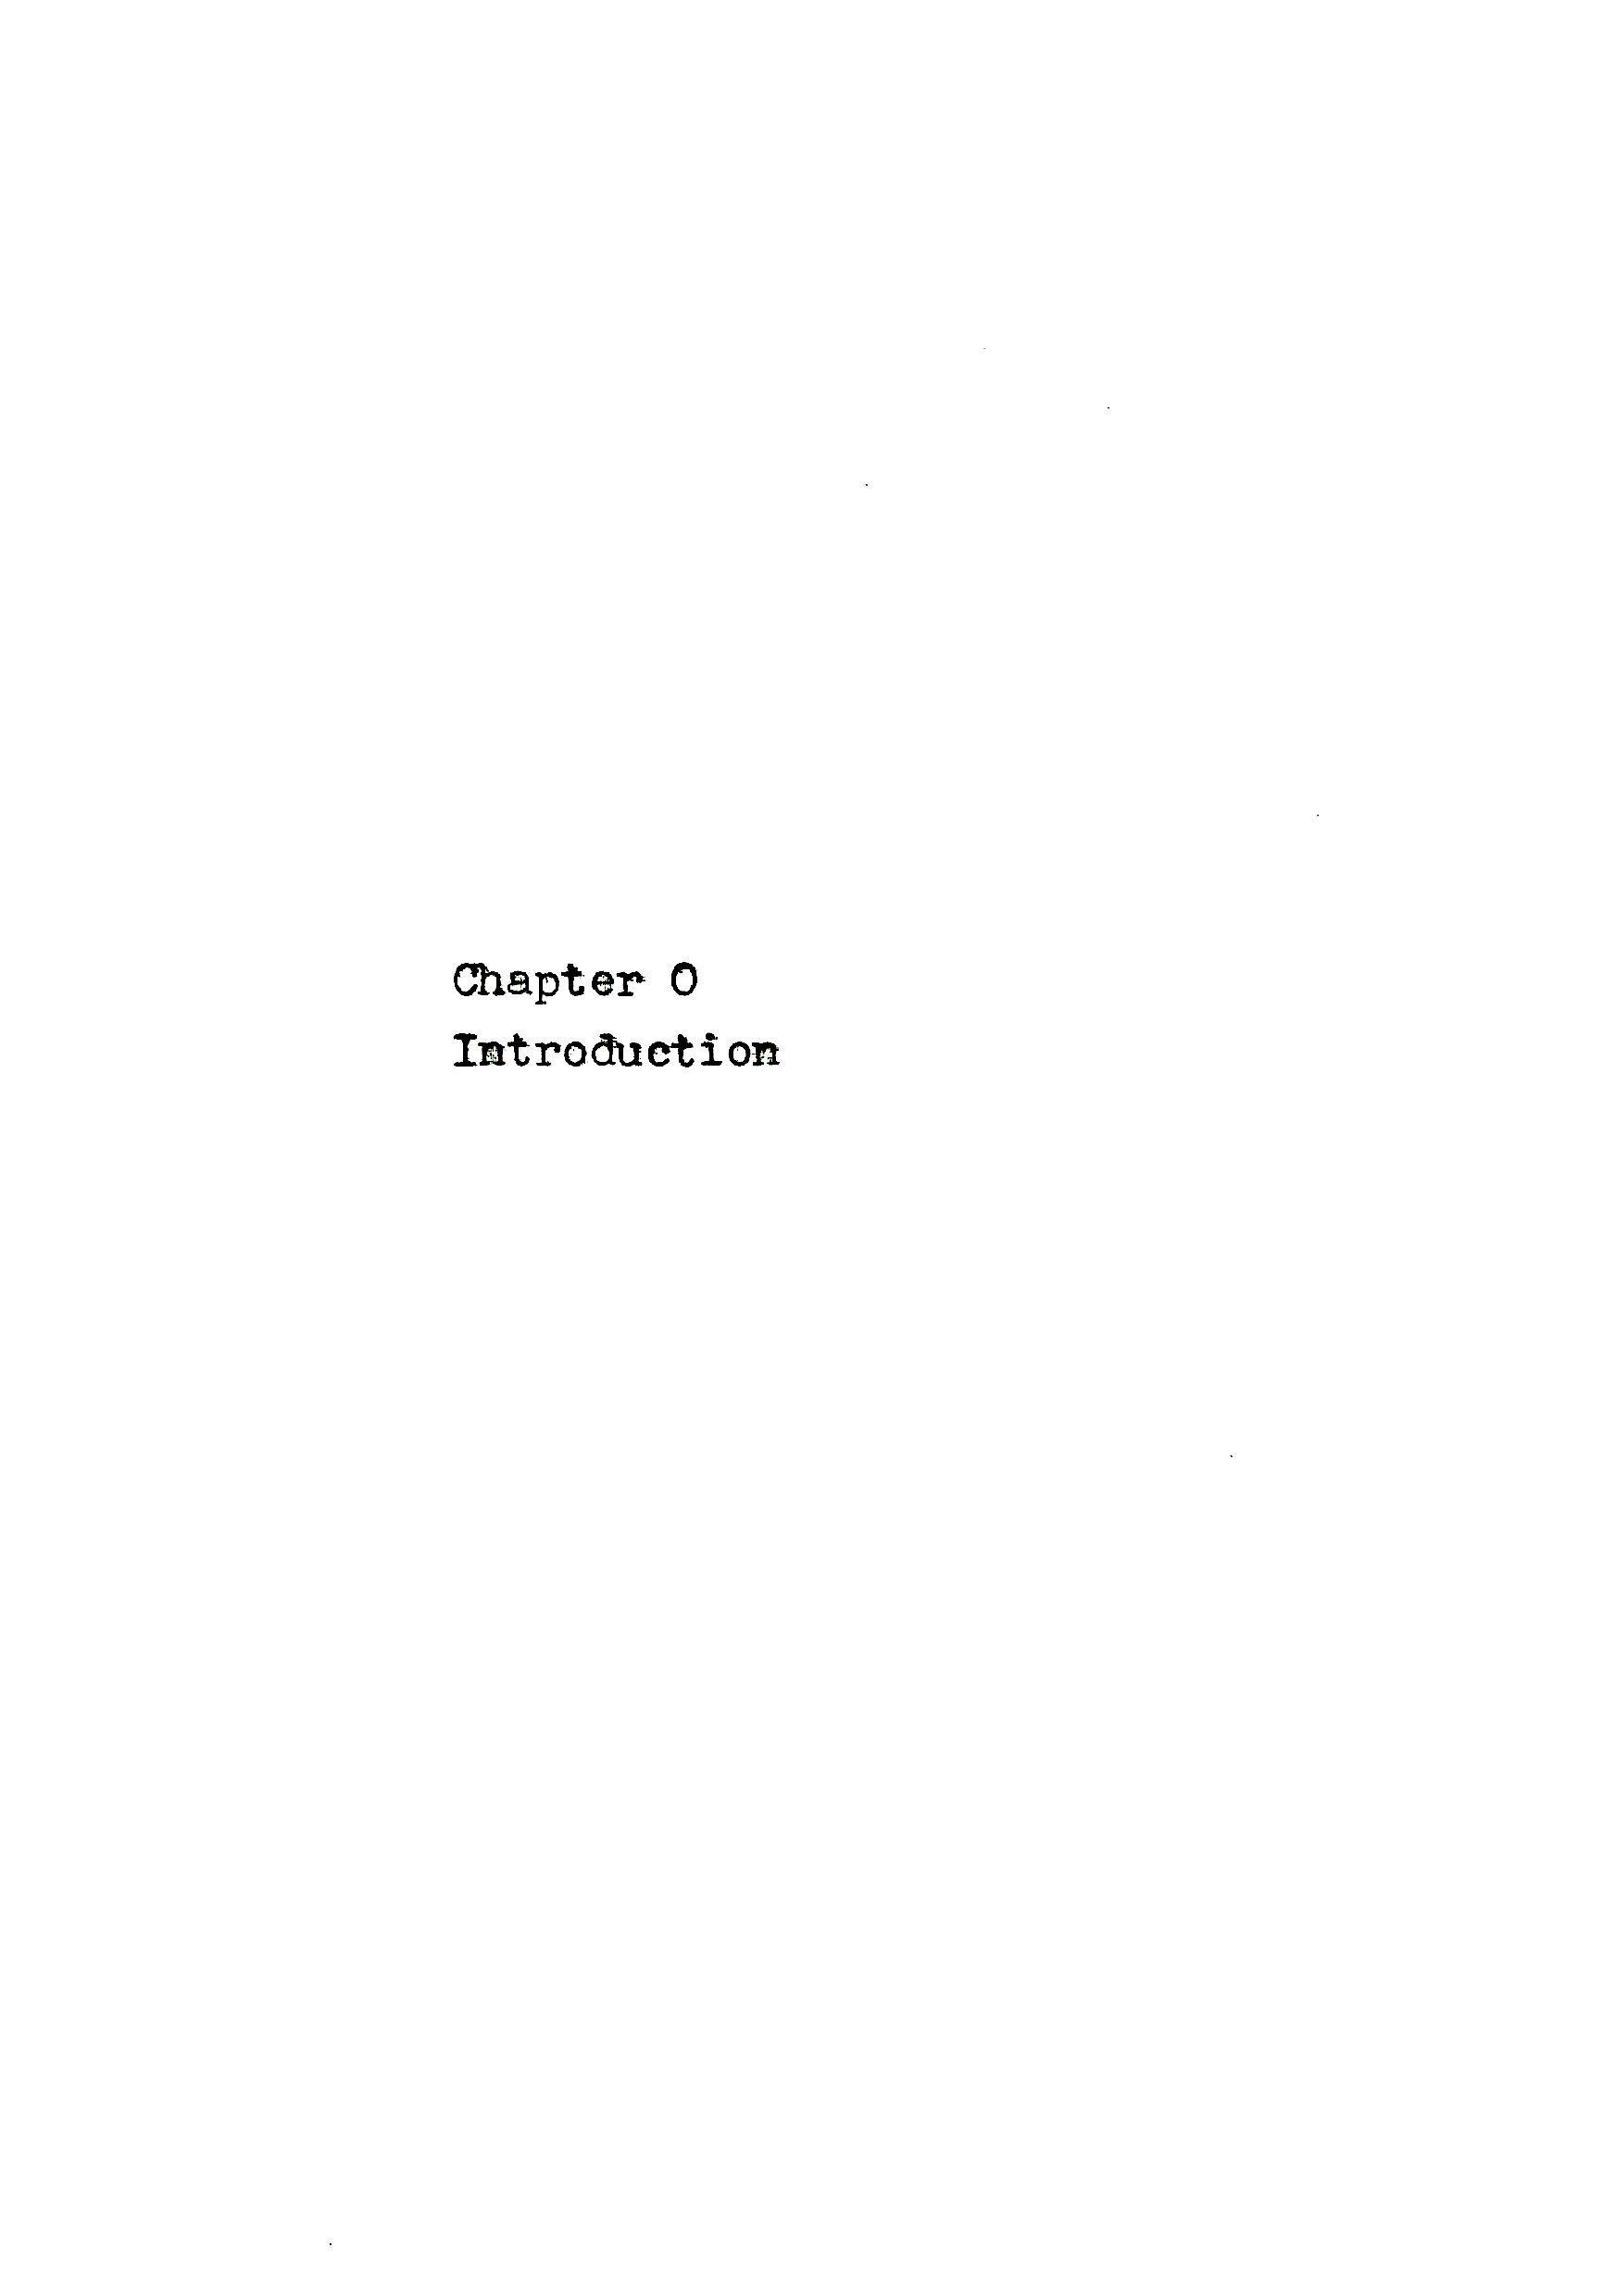
\includegraphics[%
clip,
width=1.05\paperwidth,
height=1.05\paperheight
]{chaptertitles/ch0.png}};

\clearpage

\section{The laypersons introduction}
\label{ch0:layperson}

Mathematics is one of the longest, richest and best preserved traditions humanity has ever created. It is generally accepted that mathematics has its origins in the realization that things can be counted and enumerated---that collections of things can be said to have a certain numerical size. This realization developed to the simplest theory of numbers: \emph{arithmetic}. The process of counting and doing arithmetic was used to create new knowledge and new technology: seasonal changes; lunar cycles; solar cycles; astronomy; agriculture; crop cycles; animal populations. The list could go on. Another part of mathematics came about later, when humans needed to more precisely describe the shape of land they owned---forming the field of \emph{geometry}. In fact, one of the earliest uses of the word \emph{mathematics} was by the Pythagoreans as a common name for arithmetic and geometry (\cite[1.1]{history}).

These two parts of mathematics was essentially all there was for thousands of years; in some very general way, these are still all there is to mathematics as a whole. Arithmetic and geometry continued in their own traditions all the way through antiquity and the premodern eras. This is seen, for example, in the \emph{seven liberal arts}, which acted as the educational base for students at the first universities (\cite{universities})---based on ideas dating back to Plato (\cite{plato}) and Aristotle (\cite{aristotle}). The first three, named the \emph{trivium}, consisted of grammar, rhetoric and logic. The remaining four, called the \emph{quadrivium}, consisted of music, arithmetic, geometry and astronomy.

Throughout the ages, research and the search for knowledge has undergone several revolutions; research is by now an incredibly rigorous process. The two fields of mathematics have expanded to immense sizes, and now contain hundreds upon hundreds of subfields. One of the most interesting developments---in my humble unbiased opinion---was the development of bridges, connections and similarities between geometry and arithmetic. For example, numbers---now meaning not only the numbers used for counting, but also concepts like real and complex numbers---were used by Descartes (\cite{descartes}) to make coordinate systems, where one could more easily study functions and analysis via equations. Using these coordinate systems one can build manifolds, which are geometric objects generalizing surfaces to arbitrary dimensions. 

The study of number systems eventually became the mathematical field of \emph{algebra}, while the study of shapes formed the mathematical field of \emph{topology}. It was soon discovered that using methods and techniques from algebra could greatly affect topology, leading to the field of \emph{algebraic topology}. This arguably started with Riemann studying ``connectedness numbers'' for certain spaces (\cite{riemann_1857}), an idea that was further developed by Betti (\cite{betti_1870}) and Poincaré (\cite{poincare_1895}). These numbers describe how many $n$-dimensional holes a space has. It can be difficult to imagine what holes of different dimension are, so perhaps the following comparison is useful: a circle has a hole in the middle, but so does a sphere, only that this hole is somehow of a larger dimension. The first hole is considered to be $1$-dimensional, as the hole is bound by a $1$-dimensional line; the second is considered to be $2$-dimensional, as it is bound by a $2$-dimensional surface. 

These numbers allows us to distinguish different abstract mathematical spaces. For example, if we are given two spaces $X$ and $Y$, and we can show that $X$ has a hole in dimension $13$ while $Y$ does not, then the spaces cannot be the same. The existence of holes is something that we can often compute even though we cannot visually describe the space, for example due to its large dimension. Assigning these special numbers to a space gives us a concrete computable property of it, and builds a ``bridge'' between spaces and numbers. In certain situations knowing exactly how many holes a space has of each dimension allows us to uniquely determine which space it is, so these numbers can sometimes work as a replacement for the space itself. 

The act of building connections between the two fields of mathematics is also what this thesis is about; it is about continuing the long and deep tradition of understanding the interplay of these fields. Specifically we focus on the interactions between two modern modern subfields: \emph{homological algebra} and \emph{stable homotopy theory}. The former is a subfield of algebra, where one studies the structure of the ``system of all different systems of numbers''. The latter is a subfield of topology, where one studies the structure of the ``system of all different systems of shapes''. 

We can then make a very general description of what the contents of this thesis is about: it is about studying three different bridges between stable homotopy theory and homological algebra---between shapes and numbers. These three bridges are each located in their own research paper, which form the main content of this thesis. Let us very briefly try to explain what each of these bridges are: 

The most concrete bridge comes from {\hyperref[ch1]{the first paper}}. The system of shapes at hand is in some sense a very ``fundamental'' system, as it arises as the smallest constituents---the atoms, if you will---of perhaps the most important system we have in stable homotopy theory. We directly compare this atomic system of shapes to a specific system of numbers, and prove that they are in fact equivalent; they have exactly the same structure. 

In {\hyperref[ch2]{the second paper}} the bridge is more indirect. We take a feature of certain number systems, and study an analogous concept for certain shapes. Doing this we are able to recover and generalize some already known results in topology, now seen from a completely new angle. For example, we are able to obtain two new descriptions of the atomic system we studied in the first paper. 

The bridge in {\hyperref[ch3]{the third paper}} is again quite direct, where we have a comparison between certain substructures of shapes, and certain substructures of numbers. We prove that there is a one-to-one correspondence between these collections of substructures, which provides new insight into the system of shapes that we started with. It also gives us a deeper understanding of the equivalent systems from the first paper. \newpage

\section{Central ideas}
\label{ch0:sec:Central-ideas}

As a backdrop for this entire thesis lies the ubiquitous concept of \emph{$\infty$-categories}, as developed by Joyal, Lurie and others---the canonical references being \cite{joyal_02}, \cite{lurie_09} and \cite{Lurie_HA}. We will assume familiarity with $\infty$-categories and their associated standard constructions, and use them all willy-nilly throughout the rest of the thesis. We will sometimes omit the prefix. The distinction between $\infty$-categories and classical categories should hopefully be clear from context.  

Most $\infty$-categories considered will be \emph{presentable}, in the sense of \cite[Chapter 5]{lurie_09}. 

\begin{example}
    The most important example is perhaps the $\infty$-category of \emph{spaces}, denoted $\Spaces$. This is an $\infty$-categorical version of the classical category of topological spaces. 
\end{example}

The $(\infty, 2)$-category of presentable $\infty$-categories, where the morphisms are the colimit-preserving functors, is denoted $\PrL$. It has a symmetric monoidal structure via the Lurie tensor product $\otimes^L$, and we will say a presentable $\infty$-category is \emph{presentably symmetric monoidal} if it is a commutative monoid in $\PrL$. Any such category $\C$ has a symmetric monoidal structure, with the property that the tensor product in $\C$ preserves colimits separately in each variable. The symmetric monoidal product will usually be denoted $-\otimes_\C -$, and its associated unit by $\1_\C$. 

We will also assume knowledge about \emph{stable} $\infty$-categories\index{Stable category}, which are $\infty$-categorical enhancements of triangulated categories. One can, for example, construct presentable stable $\infty$-categories from presentable $\infty$-categories via \emph{stabilization}. The stabilization of a pointed category $\mathcal{E}$ is defined by formally inverting the desuspension functor $\Omega$:
\[\Sp(\mathcal{E}) = \colim (\cdots\overset{\Omega}\to\mathcal{E}\overset{\Omega}\to\mathcal{E}).\] 
The $(\infty, 2)$-category of presentable stable $\infty$-categories and exact colimit preserving functors, denoted $\PrLs$, inherits a symmetric monoidal structure from $\PrL$. An $\infty$-category $\C$ is a \emph{presentably symmetric monoidal stable $\infty$-category} if it is a commutative monoid in $\PrLs$. This means that it is presentably symmetric monoidal, and the tensor product preserves the stable structure. 

\begin{example}
    The stabilization of the $\infty$-category of spaces is the $\infty$-category of \emph{spectra}, denoted $\Sp$. It is the unit for the Lurie tensor product on $\PrLs$, and it is the initial presentably symmetric monoidal stable $\infty$-category. The unit of the symmetric monoidal structure is the \emph{sphere spectrum} $\S$, which is the suspension spectrum of $S^0$.  
\end{example}

\begin{example}
    Another example is the derived $\infty$-category of abelian groups, $\Der(\Z)$. This is an $\infty$-categorical version of the classical triangulated derived category of $\Z$. It is a presentably symmetric monoidal stable $\infty$-category, and the unit is the integers $\Z$, treated as a chain complex concentrated in degree $0$. 
\end{example}

The derived $\infty$-category of $\Z$, as well as the $\infty$-categories of spaces, spectra, and many other interesting $\infty$-categories, satisfy some even nicer conditions than merely being presentable: they have an explicit collection of generators, which satisfy some ``smallness'' condition, defined as follows. 

\begin{definition}
    \label{ch0:def:compact-object}
    \index{Compact object}
    An object $x\in \C$ is said to be \emph{compact} if the functor $\Hom_\C(x,-)$ commutes with filtered colimits. The full subcategory of compact objects in $\C$ will be denoted $\Co$.
\end{definition}

\begin{example}
    The compact objects in $\Spaces$ are the \emph{finite spaces}, which correspond to the classical finite CW-complexes. The compact generators in $\Sp$ are the \emph{finite spectra}, where a spectrum is finite if it is the desuspension of a suspension spectrum $\Sigma^{-n}\Sigma^\infty K$ for some number $n$, where $K$ is a finite space. The compact objects in $\Der(\Z)$ are the \emph{perfect complexes}, which are the bounded complexes of finitely generated projective abelian groups. 
\end{example}

\begin{definition}
    \label{ch0:def:compactly-generated-category}
    \index{Compactly generated}
    A presentable $\infty$-category $\C$ is \emph{compactly generated} if $\Co$ generates $\C$ under filtered colimits. 
\end{definition}

All three of the categories $\Spaces$, $\Sp$ and $\Der(\Z)$ are compactly generated by their respective collection of compact objects. For the latter two, even more is true: they are compactly generated by their monoidal unit, being $\S$ and $\Z$ respectively. Such categories are sometimes called \emph{monogenic}, but we will not focus on these in this thesis. 

In the presence of symmetric monoidal structures we have another ``smallness'' condition, slightly different from being compact. As the symmetric monoidal structure is assumed to preserve colimits separately in each variable, the functor $X\otimes (-)$ has a right adjoint, denoted $\iHom_\C(X,-)$, equipping $\C$ with an \emph{internal hom} $\iHom_\C(-,-)\: \C\op\times \C\to \C$. This gives, in particular, a duality functor $(-)^\vee:=\iHom_\C(-,\1_\C)\: \C\op \to \C$, sometimes referred to as the \emph{linear dual}\index{Linear dual}. The unit map on $X^\vee$ induces by adjunction a map $X\otimes X^\vee \to \1_\C$, sometimes called the evaluation map. For any $Y\in \C$ this gives a map $X\otimes X^\vee \otimes X\to Y$, given as $ev \otimes Y$. 

\begin{definition}
    \label{ch0:def:dualizable-object}
    \index{Dualizable object}
    An object $X\in \C$ is \emph{dualizable} if for any other object $Y$, the map $X^\vee\otimes Y\to \iHom(X,Y)$, adjoint to the map $ev\otimes Y$, is an equivalence. The full subcategory of dualizable objects in $\C$ will be denoted $\C\dual$. 
\end{definition}

In a certain sense, being compact is about being small with respect to colimits, while being dualizable is about being small with respect to the monoidal structure. In very well-behaved categories, these two notions of smallness coincide. 

\begin{definition}
    \label{ch0:rigidly-generated-category}
    \index{Compactly generated!Rigid}
    A presentably symmetric monoidal stable $\infty$-category $\C$ is \emph{rigidly compactly generated} if it is compactly generated and $\Co\simeq \C\dual$. 
\end{definition}

\begin{example}
    An example is again our favorite stable $\infty$-category $\Sp$. Every compact object---being the finite spectra---is dualizable, and conversely, every dualizable object is compact. These also generate $\Sp$, hence it is a rigidly compactly generated symmetric monoidal stable $\infty$-category. Another example is the derived category $\Der(\Z)$, which is is rigidly compactly generated by the perfect complexes. 
\end{example}

\begin{remark}
    \label{ch0:rm:compacts-equal-dualizable}
    As shown in \cite[2.1.3]{hovey-palmiery-strickland_97}, a presentably symmetric monoidal $\infty$-category $\C$ is rigidly compactly generated if $\C$ is compactly generated by dualizable objects, and the unit $\1_\C$ is compact. 
\end{remark}







\subsection{Localizing subcategories and ideals}
\label{ch0:ssec:localizing-subcategories-and-ideals}

If we were to assign this thesis a single protagonist, it would be the idea of a localizing subcategory. It will heavily feature in all the different parts of the thesis: 
\begin{enumerate}
    \item In \hyperref[ch1]{paper I} we study how a specific localizing subcategory, appearing in chromatic homotopy theory, interacts with a specific homological functor.
    \item In \hyperref[ch2]{paper II} we study how, in certain situations, the category of comodules over a coalgebra in a stable $\infty$-category forms a localizing subcategory. 
    \item In \hyperref[ch3]{paper III} we prove a classification for certain localizing subcategories along nicely behaved $t$-structures on stable $\infty$-categories. 
\end{enumerate}

Given a presentable stable $\infty$-category $\C$, one should think about a localizing subcategory as being a collection of objects in $\C$, that themselves form a nice presentable stable $\infty$-category, compatible with $\C$. In other words, they are the ``structure preserving subcategories''.

\begin{definition}
    \label{ch0:def:localizing-subcategory}
    \index{Localizing subcategory}
    If $\C$ is a presentable stable $\infty$-category, then a full subcategory $\L\subseteq \C$ is \emph{localizing} if it is closed under retracts, desuspensions and colimits. 
\end{definition}

This means that $\L$ is itself a presentable stable $\infty$-category, and that computing colimits in $\L$ is equivalent to computing colimits in $\C$. 

\begin{definition}
    Let $\C$ be a presentable stable $\infty$-category. Given a collection of objects $\K\subseteq \C$ we denote by $\Loc_\C(\K)$ the smallest localizing subcategory of $\C$ containing $\K$. We will often call it the localizing subcategory \emph{generated} by $\K$. If the category $\C$ is understood, we will sometimes just write $\Loc(\K)$ for simplicity.
\end{definition}

Localizing subcategories are interconnected with the idea of ``primeness''. We give some examples for $\Der(\Z)$. 

\begin{example}
    \label{ch0:ex:p-local-ab}
    Given a chain complex of abelian groups $A$, one can form its $p$-localization $A_{(p)}$ by inverting the map $q\: A\to A$ for all other primes $q\neq p$. The derived category of all $p$-local abelian groups, denoted $\Der(\Z)^{p-\mathrm{loc}}$, is a localizing subcategory of $\Der(\Z)$. In fact, it is equivalent to $\Der(\Z_{(p)})$, the derived category of the $p$-local integers, hence also generated by $\Z_{(p)}$, treated as a complex in degree $0$. 
\end{example}

\begin{example}
    \label{ch0:ex:localizing-away-from-p}
    For a prime $p$ we can also invert only the map $p\: A\to A$, which is called localizing \emph{away} from $p$. The associated derived category denoted $\Der(\Z[\frac{1}{p}])$, is a localizing subcategory of $\Der(\Z)$. 
\end{example}

\begin{example}
    \label{ch0:ex:rational-ab}
    Inverting all primes $p$ gives the \emph{rationalization} of the complex $A$, often denoted $A_\Q$. The derived category of rational abelian groups is equivalent to the derived category of $\Q$, and is also a localizing subcategory of $\Der(\Z)$. This is also generated by the object $\Q$, treated as a chain complex in degree $0$. 
\end{example}

% \begin{example}
%     \label{ch0:ex:p-torsion-ab}
%     The $p$-power torsion of an abelian group $A$ is defined as $T_p A := \{a\in A \mid p^k a = 0 \text{ for some }k > 0\}$. There is a natural map $T_p A\to A$, and $A$ is said to be $p$-power torsion if this map is an isomorphism. The full subcategory of complexes in $\Der(\Z)$, whose homology is $p$-power torsion, denoted $\Der_{H}^p(\Z)$, is a localizing subcategory.  
% \end{example}

\begin{remark}
    \label{ch0:rm:compactly-generated-localizing-subcategory}
    \index{Localizing subcategory!Compactly generated}
    If the collection $\K \subseteq \C$ consists of only compact objects, in the sense of \cref{ch0:def:compact-object}, then the localizing subcategory $\Loc_\C(\K)$ is said to be a \emph{compactly generated} localizing subcategory. 
\end{remark}

\begin{example}
    Even though neither $\Z_{(p)}$ or $\Q$ are perfect complexes in $\Der(\Z)$, their associated localizing subcategories are in fact compactly generated. 
\end{example}

\begin{remark}
    A more rigorous way to state that a presentable stable $\infty$-category $\C$ is compactly generated---as defined in \cref{ch0:def:compactly-generated-category}---is to say that it is so if and only if the smallest localizing subcategory containing the collection of all compact objects $\Co$ is the entire $\infty$-category $\C$. In other words, there is an equivalence $\C\simeq \Loc_\C(\Co)$ of presentable stable $\infty$-categories. 
\end{remark}

If our presentable stable $\infty$-category is also symmetric monoidal, then we we want a version of localizing subcategories that preserve the monoidal structure. If one thinks of a presentably symmetric monoidal stable $\infty$-category as a categorified version of a ring, then the natural such sub-structure should model that of an ideal in a ring. 

\begin{definition}
    \label{ch0:def:localizing-ideal}
    \index{Localizing subcategory!$\otimes$-ideal}
    If $\C$ is a presentably symmetric monoidal stable $\infty$-category, then a full subcategory $\L\subseteq \C$ is a \emph{localizing $\otimes$-ideal} if it is a localizing subcategory, and for any $L\in \L$ and $X\in \C$, we have $L\otimes X\in \L$. 
\end{definition}

The definition of an ideal here is completely analogous to the classical setting of discrete rings. 

\begin{definition}
    Let $\C$ be a presentably symmetric monoidal stable $\infty$-category. Given a collection of objects $\K\subseteq \C$ we denote by $\Loc_\C^\otimes(\K)$ the smallest localizing $\otimes$-ideal of $\C$ containing $\K$. We will, as before, often refer to this as the localizing $\otimes$-ideal \emph{generated} by $\K$. 
\end{definition}

Any ideal $I$ in a discrete ring $R$ is a non-unital subring of $R$. This is also the case for a localizing $\otimes$-ideal $\L\subseteq \C$, which becomes a non-unital presentably symmetric monoidal stable $\infty$-category. However, in some good cases $\L$ is actually unital, but the unit $\1_\L$ will naturally have to be different than the unit $\1_\C$, otherwise we would have $\L=\C$. The localizing ideals we study in \cref{ch1}, as well as some of the ones in \cref{ch2}, will have this property. In particular, as we will see in the next section, any localizing $\otimes$-ideal which is compactly generated in the sense of \cref{ch0:rm:compactly-generated-localizing-subcategory} will have this property.

\begin{example}
    The examples we saw earlier, \cref{ch0:ex:p-local-ab} and \cref{ch0:ex:rational-ab}, are all localizing $\otimes$-ideals. We will see in the next section that they, or some slight variation of these categories, are compactly generated localizing $\otimes$-ideals, which by the above comment mean they are all presentably symmetric monoidal stable $\infty$-categories themselves. 
\end{example}





\subsection{Local duality}
\label{ch0:ssec:local-duality}

The theory of abstract local duality, proved in \cite{hovey-palmiery-strickland_97} and generalized to the $\infty$-categorical setting in \cite{barthel-heard-valenzuela_2018}, is one of the central ideas of this thesis that will show up several times. 

\subsubsection{Localizations}

To understand local duality, and also the use of localizing subcategories, we look at certain functors, called localizations. In spirit, these are functors that invert a certain class of maps. 

\begin{definition}
    \label{ch0:def:localization}
    \index{Localization}
    Let $\C$ and $\D$ be two presentable stable $\infty$-categories. A \emph{localization} is a colimit preserving functor $f\colon \C\longrightarrow \D$ such that the right adjoint $i$ is fully faithful.  
\end{definition}

There are several ways to construct localizations, but one method particularly important for us will be via localizing subcategories. 

\begin{definition}
    \label{ch0:def:right-orthogonal-complement}
    \index{Right orthogonal complement}
    Let $\L\subseteq \C$ be a full subcategory. The \emph{right orthogonal complement} of $\L$, is the full subcategory $\L^\perp$ consisting of objects $X\in \C$ such that $\Hom_\C(L,X)\simeq 0$ for all $L\in \L$.  
\end{definition}

\begin{example}
    \label{ch0:ex:localization-from-localizing-subcategory}
    Let $\L\subseteq \C$ be a localizing subcategory. The inclusion of the complement $\L^\perp \hookrightarrow \C$ is fully faithful and has a left adjoint $f\colon \C\longrightarrow \L^\perp$. Hence, $f$ is a localization, and its kernel is precisely $\L$. 
\end{example}

\begin{example}
    \label{ch0:ex:derived-p-completion}
    Let $\C=\Der(\Z)$ and $\L = \Der(\Z[\frac{1}{p}])$ as in \cref{ch0:ex:localizing-away-from-p}. The right orthogonal complement is the category of derived $p$-complete abelian groups, $\Der(\Z)^{p-\mathrm{comp}}$. The associated localization $\Lambda_p$ is the total left derived functor of the $p$-adic completion functor $C^p$, defined by sending an abelian group $A$ to the colimit $A^\wedge_p = \colim_k A/p^k$. In other words, we have a localization 
    \[\Lambda_p \simeq \bbL C^p \: \Der(\Z)\to \Der(\Z)^{p-\mathrm{comp}}.\]
\end{example}

We will mostly focus on localizations of presentably symmetric monoidal stable $\infty$-categories, hence we also want to make sure that the localizations of interest preserve the monoidal structure. This is done as follows. 

\begin{definition}
    \label{ch0:def:L-equivalence}
    Let $\C$ and $\D$ be two presentably symmetric monoidal stable $\infty$-categories and $f\colon \C\longrightarrow \D$ a functor. A map $\phi$ in $\C$ is called an \emph{$f$-equivalence} if $f(\phi)$ is an equivalence. The functor $f$ is said to be \emph{tensor-compatible} if being an $f$-equivalence is stable under tensor product: in the sense that for any $f$-equivalence $X\longrightarrow Y$ and object $Z\in \C$, the induced map $X\otimes Z\longrightarrow Y\otimes Z$ is again an $f$-equivalence. 
\end{definition}

\begin{definition}
    \label{ch0:def:monoidal-localization}
    \index{Localization}
    Let $\C$ and $\D$ be two presentably symmetric monoidal stable $\infty$-categories. A \emph{monoidal localization} is a tensor-compatible functor $f\colon \C\longrightarrow \D$ with a fully faithful right adjoint $i$. 
\end{definition}

\begin{remark}
    \label{ch0:rm:localizations-tensor-compatible}
    For the rest of this thesis we will assume that, whenever $\C$ is a presentably symmetric monoidal, that any localization of $\C$ is tensor-compatible. We will usually omit the prefix ``monoidal'' from localizations. It is really only in \hyperref[ch3]{paper III} that we will see non-monoidal localizations, hence the distinction between them should hopefully be clear from the context.
\end{remark}

\begin{remark}
    Let $f\colon \C\longrightarrow \D$ be a localization. The composition of $f$ with the fully faithful right adjoint $i$ is denoted $L$. The functor $i$ gives an equivalence between $\D$ and a full subcategory of $\C$, denoted $\C_L$. By \cite[5.2.7.4]{lurie_09} there is an equivalence between localizations $f\colon \C\longrightarrow \D$ and functors $L\colon \C\longrightarrow \C_L$ ($L$ viewed as a functor to its essential image) that are left adjoint to the inclusion. We will usually use this perspective, using the functor $L$ rather than $f$. 
\end{remark}

\begin{definition}
    \index{Local object}
    Given a localization $L\colon \C\longrightarrow \C_L$, any object $X\in \C$ admits a map $X\longrightarrow LX$ coming from the unit of the adjunction, called its \emph{$L$-localization}. The object $X$ is said to be \emph{$L$-local} if this is an $L$-equivalence. By definition the category of $L$-local objects is $\C_L$. 
\end{definition}

\begin{proposition}[{\cite[1.3.4.3]{Lurie_HA}}]
    If $L\colon \C\longrightarrow \C_L$ is a localization, then the category of local objects $\C_L$ is equivalent to the full subcategory of $\C$ obtained by inverting the collection of $L$-equivalences $W_L$. In other words, there is an equivalence of symmetric monoidal stable $\infty$-categories $\C_L\simeq \C[W_L^{-1}]$.
\end{proposition}

\begin{remark}
    \label{ch0:rm:monoidal-localization}
    Let $L\colon \C\longrightarrow \C_L$ be a localization on a presentably symmetric monoidal stable $\infty$-category $\C$. The symmetric monoidal structure on $\C$ induces a symmetric monoidal structure on $\C_L$, defined by $L(-\otimes_\C -)$, making $L$ into a symmetric monoidal functor. This follows from \cite[2.2.1.9]{Lurie_HA} by our standing assumption that all localizations on symmetric monoidal categories are tensor-compatible, see \cref{ch0:rm:localizations-tensor-compatible}. 
\end{remark}

\begin{remark}
    If $L\: \C\to \C_L$ is a monoidal localization, then the kernel $\Ker L$ is a localizing $\otimes$-ideal of $\C$. 
\end{remark}

\begin{remark}
    \index{Colocalization}
    Similarly to localizations, we can define \emph{colocalizations} as functors $g\colon \C\longrightarrow \D$ admitting a fully faithful left adjoint $i$. The composition $i\circ g$ is denoted $\Gamma$. The adjoint gives an equivalence between $\D$ and a full subcategory $\C^\Gamma$ of $\C$, and the datum of a colocalization is equivalent to the datum of a functor $\Gamma\colon \C\longrightarrow \C^\Gamma$ that is right adjoint to the inclusion. Dually to localizations, we get for any $X\in \C$ a colocalization map $\Gamma X\to X$, and we say $X$ is \emph{$\Gamma$-colocal}\index{Colocal object} if this is an equivalence. 
\end{remark}

Let $\C$ be a presentably symmetric monoidal stable $\infty$-category. For any localization $L\colon \C\longrightarrow \C_L$, the image of the unit $L\1_\C$ is a ring object, and any $L$-local object $X$ admits the structure of an $L\1_\C$ module via the map of functors $L\1_\C \otimes L(-)\longrightarrow L(-)$. 

\begin{remark}
    \label{ch0:rm:L1-module-adjoint-map}
    By the tensor-internal hom adjunction, the $L\1_\C$-module structure on an $L$-local object $X$ is equivalent to a map $L(-)\longrightarrow \iHom(L\1_\C,-)$. 
\end{remark}

\begin{definition}
    \label{ch0:def:smashing-localization}
    \index{Localization!Smashing}
    We say a localization $L$ is \emph{smashing} if the $L\1_\C$-module map above is an equivalence. This is equivalent to the dual map $L(-)\longrightarrow \iHom_\C(L\1, -)$ being an equivalence. 
\end{definition}

\begin{example}
    \label{ch0:ex:p-localization-ab-smashing}
    There is a $p$-localization functor $L\:\Der(\Z)\to \Der(\Z_{(p)})$ given by inverting all primes $q\neq p$. This is a smashing localization, and is then given by $L \simeq \Z_{(p)}\otimes_\Z (-)$. 
\end{example}

\begin{remark}
    \label{ch0:rm:smashing-then-modules-over-unit}
    For a smashing localization $L$ we have by definition that being $L$-local is equivalent to being a module over $L\1_\C$. This gives a symmetric monoidal equivalence $\C_L \simeq \Mod_{L\1_\C}(\C)$. 
\end{remark}

\begin{remark}
    \label{ch0:rm:smashing-colocalization}
    \index{Colocalization!Smashing}
    Similarly, for a colocalization $\Gamma$ there are maps $\Gamma \1_\C \otimes \Gamma(-)\longrightarrow \Gamma (-)$ and $\Gamma(-)\longrightarrow \iHom(\Gamma \1_\C, -)$. The colocalization $\Gamma$ is said to be \emph{smashing} if the former is an equivalence. In \cref{ch0:rm:L1-module-adjoint-map} we noted that for a localization the module structure was equivalent to a map into $\iHom(L\1_\C,-)$. For colocalizations this is no longer true, leading to two different notions of ``modules'' in this setting. This setup is studied in detail in \hyperref[ch2]{paper II}. 
\end{remark}

\begin{remark}
    Any monoidal localization $L$ equips $\C_L$ with a symmetric monoidal structure, as seen in \cref{ch0:rm:monoidal-localization}. If $L$ is a smashing localization, then the induced tensor product is the same as in the category $\C$. The same applies to smashing colocalizations. 
\end{remark}





\subsubsection{The local duality theorem}

We are now ready to present the setup for local duality, which is a natural duality theory for compactly generated localizing $\otimes$-ideals. 

\begin{definition}
    \label{ch0:def:local-duality-context}
    \index{Local duality!Context}
    A pair $(\C, \K)$, consisting of a presentably symmetric monoidal stable $\infty$-category $\C$, that is compactly generated by dualizable objects, and a subset $\K\subseteq \Co$, is called a \emph{local duality context}.
\end{definition}

Any choice of local duality context allows us to assign to it three new categories, which together decomposes the category $\C$. 

\begin{construction}
    \label{ch0:const:local-duality-categories}
    \index{Local duality!Torsion}
    \index{Local duality!Torsion objects}
    \index{Local duality!Local objects}
    \index{Local duality!Complete objects}
    Let $(\C, \K)$ be a local duality context. We define the category of \emph{$\K$-torsion objects} in $\C$ to be the localizing $\otimes$-ideal generated by $\K$, and denote it by $\C\Ktors:= \Loc_\C^\otimes(\K)$. Further we define the category of \emph{$\K$-local objects} in $\C$ to be the right orthogonal complement---see \cref{ch0:def:right-orthogonal-complement}---of $\C\Ktors$. In other words $\C\Kloc := (\C\Ktors)^\perp$. Finally we define the category of \emph{$\K$-complete objects} in $\C$ to be the right orthogonal complement of $\C\Kloc$, i.e., $\C\Kcomp= (\C\Kloc)^\perp$. 
    
    These three categories have fully faithful inclusions into $\C$, denoted $i_{\K-\mathrm{tors}}$, $i_{\K-\mathrm{loc}}$ and $i_{\K-\mathrm{comp}}$ respectively. By the adjoint functor theorem, \cite[5.5.2.9]{lurie_09}, the inclusions $i_{\K-\mathrm{loc}}$ and $i_{\K-\mathrm{comp}}$ have left adjoints $L_\K$ and $\Lambda_\K$ respectively, while $i_{\K-\mathrm{tors}}$ and $i_{\K-\mathrm{loc}}$ have right adjoints $\Gamma_\K$ and $V_\K$ respectively. These are then, by definition, localizations and colocalizations. 
    
    The torsion, local and complete objects all form $\otimes$-ideals, meaning that the localizations and colocalizations above are compatible with the symmetric monoidal structure of $\C$, in the sense of \cref{ch0:def:L-equivalence}. In particular, by \cref{ch0:rm:monoidal-localization} the categories inherit unique induced symmetric monoidal structures such that $L_\K$, $\Lambda_\K$, $\Gamma_\K$ and $V_\K$ are symmetric monoidal functors. 

    For any $X\in \C$, these functors assemble into two cofiber sequences:
    \[\Gamma_\K X \longrightarrow X \longrightarrow L_\K X \quad \text{and}\quad V_\K X \longrightarrow X \longrightarrow \Lambda_\K X.\]
    Note also that these functors only depend on the localizing subcategory $\C\Ktors$, not on the particular choice of generators $\K$. Thus, when the set $\K$ is clear from the context, we sometimes omit it as a subscript when writing the functors. 
\end{construction}

\begin{remark}
    \label{ch0:rm:tors-loc-comp-compactly-generated}
    By definition $\C\Ktors$ is compactly generated, and by \cite[2.17]{barthel-heard-valenzuela_2018} both $\C\Kloc$ and $\C\Kcomp$ are as well. 
\end{remark}

The following theorem is a slightly simplified version of the abstract local duality theorem of \cite[3.3.5]{hovey-palmiery-strickland_97} and \cite[2.21]{barthel-heard-valenzuela_2018}.  

\begin{theorem}
    \label{ch0:thm:local-duality}
    \index{Local duality!Theorem}
    If $(\C, \K)$ is a local duality context, then
    \begin{enumerate}
        \item $\Gamma$ is a smashing colocalization and $L$ is a smashing localization,
        \item there are equivalences of functors $\Lambda \simeq \iHom(\Gamma \1,-)$ and $V \simeq \iHom(L\1, -)$, and
        \item the functors 
        \[\Gamma\colon \C\Kcomp\longrightarrow \C\Ktors \text{ and } \Lambda\colon \C\Ktors\longrightarrow \C\Kcomp\]
        are mutually inverse equivalences of symmetric monoidal stable $\infty$-categories.
    \end{enumerate}
    This can be summarized by the following diagram of adjoints\index{Local duality!Diagram}
    \begin{center}
        \begin{tikzcd}
                & {\C\Kloc} \\
                & {\C} \\
                {\C\Ktors} && {\C\Kcomp}
                \arrow["L", xshift=-4pt, from=2-2, to=1-2]
                \arrow[from=1-2, to=2-2]
                \arrow["V", xshift=4pt, from=2-2, to=1-2, swap]

                \arrow["\Lambda", yshift=2pt, xshift=2pt, from=2-2, to=3-3]
                \arrow[yshift=-2pt, xshift=0pt, from=3-3, to=2-2]

                \arrow["\Gamma", yshift=-2pt, xshift=0pt, from=2-2, to=3-1]
                \arrow[yshift=2pt, xshift=-2pt, from=3-1, to=2-2]
                
                \arrow[bend left=35, dashed, from=3-1, to=1-2]
                \arrow[bend left=35, dashed, from=1-2, to=3-3]

                \arrow["\simeq"', swap, from=3-1, to=3-3]
        \end{tikzcd}    
    \end{center}
\end{theorem}

\begin{remark}
    \label{ch0:rm:monoidal-structure-in-local-duality}
    \cref{ch0:thm:local-duality} implies, in particular, that the symmetric monoidal structure induced by the localization $L$ and the colocalization $\Gamma$ is just the symmetric monoidal structure on $\C$ restricted to the full subcategories. This is not the case for $\C\Kcomp$, where the symmetric monoidal structure is given by $\Lambda(-\otimes_\C-)$. The functor $V$ also induces a symmetric monoidal structure on $\C\Kloc$, but this coincides with the one induced by $L$, due to their associated endofunctors on $\C$ defining an adjoint symmetric monoidal monad-comonad pair. Note that we will not need or focus on the functor $V$, hence it will usually be omitted from the local duality diagrams for the rest of the thesis. 
\end{remark}

\begin{example}
    The object $\Z_{(p)}/p \cong \F_p$ is compact in the derived category of $p$-local abelian groups, $\Der(\Z_{(p)})$. This means that $(\Der(\Z_{(p)}), \K)$ forms a local duality context, where $\K$ is the singleton set $\{\F_p\}$. The category of local objects, $\Der(\Z_{(p)})\Kloc$, has objects in which $p$ is invertible. But, as all other primes are already invertible, all of these are necessarily rational, giving $\Der(\Z_{(p)})\Kloc \simeq \Der(\Q)$. The category $\Der(\Z_{(p)})\Ktors$ is equivalent to the category of derived $p$-torsion objects in $\Der(\Z_{(p)})$. Dually, the category $\Der(\Z_{(p)})\Kcomp$ is equivalent to the derived $p$-complete objects in $\Der(\Z)_{(p)}$, which gives a local duality diagram 
    \begin{center}
        \begin{tikzcd}
            & {\Der(\Q)} \\
            & {\Der(\Z_{(p)})} \\
            {\Der(\Z_{(p)})^{p-\mathrm{tors}}} && {\Der(\Z_{(p)})^{p-\mathrm{comp}}}
            \arrow["L_p", xshift=-2pt, from=2-2, to=1-2]
            \arrow[xshift=2pt, from=1-2, to=2-2]

            \arrow["\Delta_p", yshift=2pt, xshift=2pt, from=2-2, to=3-3]
            \arrow[yshift=-2pt, xshift=0pt, from=3-3, to=2-2]

            \arrow["\Gamma^p", yshift=-2pt, xshift=0pt, from=2-2, to=3-1]
            \arrow[yshift=2pt, xshift=-2pt, from=3-1, to=2-2]

            \arrow[bend left=35, dashed, from=3-1, to=1-2]
            \arrow[bend left=35, dashed, from=1-2, to=3-3]

            \arrow["\simeq"', swap, from=3-1, to=3-3]
        \end{tikzcd}    
    \end{center}
\end{example}









































































\subsection{Chromatic homotopy theory}
\label{ch0:ssec:chromatic-homotopy-theory}

In the abstract we mentioned that the overarching goal of the thesis is to understand aspects of monochromatic homotopy theory. To do this we first need to situate ourselves into the chromatic viewpoint of stable homotopy theory; our approach is inspired by \cite{barthel-beaudry_19}, and will particularly try to tie it to the ideas already introduced. 

In very crude words one can describe chromatic homotopy theory as a reductionist perspective---or maybe a toolbox---for studying the $\infty$-category of spectra, $\Sp$, in which one decomposes it to its smallest fundamental pieces. An often repeated analogy is that of a prism. If $\Sp$ consists of white light, then shining it through the ``chromatic lens'' decomposes it to distinct colors, labeled by a non-negative integer $n$ called the \emph{chromatic height}, analogous to the wavelength of a light wave. 

\begin{center}
\tikzset{every picture/.style={line width=0.75pt}} %set default line width to 0.75pt   

\begin{tikzpicture}[x=1pt,y=1pt,yscale=-1,xscale=1]
    %uncomment if require: \path (0,300); %set diagram left start at 0, and has height of 300
    
%Shape: Triangle [id:dp28924046358844724] 
\draw  [color={rgb, 255:red, 128; green, 128; blue, 128 }  ,draw opacity=1 ][line width=1.5]  (320.22,100) -- (370,190) -- (270,190) -- cycle ;
    %Shape: Wave [id:dp4206352155629708] 
    \draw   (192.8,151.3) .. controls (193.62,152.48) and (194.4,153.6) .. (195.3,153.6) .. controls (196.2,153.6) and (196.98,152.48) .. (197.8,151.3) .. controls (198.62,150.12) and (199.4,149) .. (200.3,149) .. controls (201.2,149) and (201.98,150.12) .. (202.8,151.3) .. controls (203.62,152.48) and (204.4,153.6) .. (205.3,153.6) .. controls (206.2,153.6) and (206.98,152.48) .. (207.8,151.3) .. controls (208.62,150.12) and (209.4,149) .. (210.3,149) .. controls (211.2,149) and (211.98,150.12) .. (212.8,151.3) .. controls (213.62,152.48) and (214.4,153.6) .. (215.3,153.6) .. controls (216.2,153.6) and (216.98,152.48) .. (217.8,151.3) .. controls (218.62,150.12) and (219.4,149) .. (220.3,149) .. controls (221.2,149) and (221.98,150.12) .. (222.8,151.3) .. controls (223.62,152.48) and (224.4,153.6) .. (225.3,153.6) .. controls (226.2,153.6) and (226.98,152.48) .. (227.8,151.3) .. controls (228.62,150.12) and (229.4,149) .. (230.3,149) .. controls (231.2,149) and (231.98,150.12) .. (232.8,151.3) .. controls (233.62,152.48) and (234.4,153.6) .. (235.3,153.6) .. controls (236.2,153.6) and (236.98,152.48) .. (237.8,151.3) .. controls (238.62,150.12) and (239.4,149) .. (240.3,149) .. controls (241.2,149) and (241.98,150.12) .. (242.8,151.3) .. controls (243.62,152.48) and (244.4,153.6) .. (245.3,153.6) .. controls (246.2,153.6) and (246.98,152.48) .. (247.8,151.3) .. controls (248.62,150.12) and (249.4,149) .. (250.3,149) .. controls (251.2,149) and (251.98,150.12) .. (252.8,151.3) .. controls (253.62,152.48) and (254.4,153.6) .. (255.3,153.6) .. controls (256.2,153.6) and (256.98,152.48) .. (257.8,151.3) .. controls (258.62,150.12) and (259.4,149) .. (260.3,149) .. controls (261.2,149) and (261.98,150.12) .. (262.8,151.3) .. controls (263.62,152.48) and (264.4,153.6) .. (265.3,153.6) .. controls (266.2,153.6) and (266.98,152.48) .. (267.8,151.3) .. controls (268.62,150.12) and (269.4,149) .. (270.3,149) .. controls (271.2,149) and (271.98,150.12) .. (272.8,151.3) .. controls (273.62,152.48) and (274.4,153.6) .. (275.3,153.6) .. controls (276.2,153.6) and (276.98,152.48) .. (277.8,151.3) .. controls (278.62,150.12) and (279.4,149) .. (280.3,149) .. controls (281.2,149) and (281.98,150.12) .. (282.8,151.3) .. controls (283.62,152.48) and (284.4,153.6) .. (285.3,153.6) .. controls (286.2,153.6) and (286.98,152.48) .. (287.8,151.3) .. controls (288.62,150.12) and (289.4,149) .. (290.3,149) .. controls (291.2,149) and (291.98,150.12) .. (292.8,151.3) .. controls (293.62,152.48) and (294.4,153.6) .. (295.3,153.6) .. controls (296.2,153.6) and (296.98,152.48) .. (297.8,151.3) .. controls (298.62,150.12) and (299.4,149) .. (300.3,149) .. controls (301.2,149) and (301.98,150.12) .. (302.8,151.3) .. controls (303.62,152.48) and (304.4,153.6) .. (305.3,153.6) .. controls (306.2,153.6) and (306.98,152.48) .. (307.8,151.3) .. controls (308.62,150.12) and (309.4,149) .. (310.3,149) .. controls (311.2,149) and (311.98,150.12) .. (312.8,151.3) .. controls (313.62,152.48) and (314.4,153.6) .. (315.3,153.6) .. controls (316.2,153.6) and (316.98,152.48) .. (317.8,151.3) .. controls (318.62,150.12) and (319.4,149) .. (320.3,149) .. controls (320.33,149) and (320.37,149) .. (320.4,149) ;
    %Straight Lines [id:da3725009850844284] 
    \draw [color={rgb, 255:red, 208; green, 2; blue, 27 }  ,draw opacity=1 ]   (320,150) -- (448.18,90.84) ;
    \draw [shift={(450,90)}, rotate = 155.22] [color={rgb, 255:red, 208; green, 2; blue, 27 }  ,draw opacity=1 ][line width=0.75]    (10.93,-3.29) .. controls (6.95,-1.4) and (3.31,-0.3) .. (0,0) .. controls (3.31,0.3) and (6.95,1.4) .. (10.93,3.29)   ;
    %Straight Lines [id:da04393101077336736] 
    \draw [color={rgb, 255:red, 245; green, 166; blue, 35 }  ,draw opacity=1 ]   (320,150) -- (448.09,110.59) ;
    \draw [shift={(450,110)}, rotate = 162.9] [color={rgb, 255:red, 245; green, 166; blue, 35 }  ,draw opacity=1 ][line width=0.75]    (10.93,-3.29) .. controls (6.95,-1.4) and (3.31,-0.3) .. (0,0) .. controls (3.31,0.3) and (6.95,1.4) .. (10.93,3.29)   ;
    %Straight Lines [id:da6751899671862938] 
    \draw [color={rgb, 255:red, 248; green, 231; blue, 28 }  ,draw opacity=1 ]   (320,150) -- (448.02,130.3) ;
    \draw [shift={(450,130)}, rotate = 171.25] [color={rgb, 255:red, 248; green, 231; blue, 28 }  ,draw opacity=1 ][line width=0.75]    (10.93,-3.29) .. controls (6.95,-1.4) and (3.31,-0.3) .. (0,0) .. controls (3.31,0.3) and (6.95,1.4) .. (10.93,3.29)   ;
    %Straight Lines [id:da7243327342564972] 
    \draw [color={rgb, 255:red, 126; green, 211; blue, 33 }  ,draw opacity=1 ]   (320,150) -- (448,150) ;
    \draw [shift={(450,150)}, rotate = 180] [color={rgb, 255:red, 126; green, 211; blue, 33 }  ,draw opacity=1 ][line width=0.75]    (10.93,-3.29) .. controls (6.95,-1.4) and (3.31,-0.3) .. (0,0) .. controls (3.31,0.3) and (6.95,1.4) .. (10.93,3.29)   ;
    %Straight Lines [id:da7878005985339279] 
    \draw [color={rgb, 255:red, 74; green, 144; blue, 226 }  ,draw opacity=1 ]   (320,150) -- (448.02,169.7) ;
    \draw [shift={(450,170)}, rotate = 188.75] [color={rgb, 255:red, 74; green, 144; blue, 226 }  ,draw opacity=1 ][line width=0.75]    (10.93,-3.29) .. controls (6.95,-1.4) and (3.31,-0.3) .. (0,0) .. controls (3.31,0.3) and (6.95,1.4) .. (10.93,3.29)   ;
    %Straight Lines [id:da4893685373249388] 
    \draw [color={rgb, 255:red, 144; green, 19; blue, 254 }  ,draw opacity=1 ]   (320,150) -- (448.13,199.28) ;
    \draw [shift={(450,200)}, rotate = 201.04] [color={rgb, 255:red, 144; green, 19; blue, 254 }  ,draw opacity=1 ][line width=0.75]    (10.93,-3.29) .. controls (6.95,-1.4) and (3.31,-0.3) .. (0,0) .. controls (3.31,0.3) and (6.95,1.4) .. (10.93,3.29)   ;
    %Straight Lines [id:da9572748849226034] 
    \draw    (320,150) ;
    \draw [shift={(320,150)}, rotate = 0] [color={rgb, 255:red, 0; green, 0; blue, 0 }  ][fill={rgb, 255:red, 0; green, 0; blue, 0 }  ][line width=0.75]      (0, 0) circle [x radius= 1.34, y radius= 1.34]   ;
    
    % Text Node
    \draw (280,192.4) node [anchor=north west][inner sep=0.75pt]   [align=left] {Chromatic lens};
    % Text Node
    \draw (172,145) node [anchor=north west][inner sep=0.75pt]    {$\Sp$};
    % Text Node
    \draw (451,195.4) node [anchor=north west][inner sep=0.75pt]    {$\C_{0}$};
    % Text Node
    \draw (451,82.4) node [anchor=north west][inner sep=0.75pt]    {$\C_{\infty }$};
    % Text Node
    \draw (451,165.4) node [anchor=north west][inner sep=0.75pt]    {$\C_{1}$};
    % Text Node
    \draw (451,123.4) node [anchor=north west][inner sep=0.75pt]    {$\C_{n}$};
    % Text Node
    \draw (453,99.4) node [anchor=north west][inner sep=0.75pt]    {$\vdots $};
    % Text Node
    \draw (453,140.4) node [anchor=north west][inner sep=0.75pt]    {$\vdots $};
    
    
    \end{tikzpicture}
\end{center}

The key to this perspective is that the individual pieces of information can be reassembled back to give information about $\Sp$. This happens in the form of a filtration on the sphere spectrum $\S$, called the \emph{chromatic filtration}. The colimit of this filtration recovers the sphere, hence we can think of the main idea of chromatic homotopy theory as the following: in order to understand $\Sp$, it should be enough to understand the ``chromatic pieces'' individually. 

\begin{remark}
    \label{ch0:rm:quillen-formal-groups}
    Historically these chromatic pieces came about from the relationship between spectra and the algebraic geometry of formal groups, as studied by Quillen in his seminal paper \cite{quillen_1969}. To any complex oriented ring spectrum $E$, one can associate to it a formal group, see for example \cite[Appendix 2]{ravenel_86}. Quillen proved that the formal group associated to the complex cobordism spectrum $\MU$ is the universal formal group over the Lazard ring. The moduli stack of formal groups has a filtration by the \emph{height} of a formal group, and pulling back this filtration to spectra gives precisely the chromatic filtration hinted to above. 
\end{remark}

\subsubsection{Fracture squares and field objects}
\label{ch0:sssec:fracture-squares}

In light of Waldhausen's viewpoint of stable homotopy theory as an enhancement of algebra, usually called \emph{brave new algebra}, one should view the category of spectra $\Sp$ as a homotopical enrichment of the derived category of abelian groups $\Der(\Z)$. We have seen earlier that abelian groups can be studied one prime at the time, which corresponds to studying $\Der(\Z_{(p)})$, the $p$-local derived category. We also want to do this in spectra. 

In \cite{bousfield_1979_localization} Bousfield developed a general machinery for studying localizations on $\Sp$, by inverting maps that are equivalences after tensoring with some spectrum $F$, now called \emph{Bousfield localizations}. The corresponding localization functor is usually denoted $L_F$. 

\begin{example}
    \index{p-localization}
    We can create a version of $p$-localization on $\Sp$, by Bousfield localizing at the $p$-local Moore spectrum $M\Z_{(p)}$, giving a functor usually written 
    \[L_{(p)} \:\Sp \to \Sp_{(p)}.\] 
    On homotopy groups this has the effect of $p$-localizing, in the sense that 
    \[\pi_* L_{(p)}X \simeq \pi_* X [S^{-1}]\simeq \pi_* X \otimes \Z_{(p)}\]
    where $S$ is the set of all primes $q\neq p$. The category of $p$-local spectra, denoted $\Sp_{(p)}$, should then be thought of as a homotopical enrichment of $\Der(\Z_{(p)})$. Just as in \cref{ch0:ex:p-localization-ab-smashing}, the $p$-localization functor $L_{(p)}$ is a smashing localization. 
\end{example}


% \begin{construction}
%     \label{const:bousfield-localization}
%     Let $F$ be a spectrum and $f\colon X\longrightarrow Y$ a map of spectra. We say $f$ is an {\defn $F$-equivalence}, if $f\otimes F$ is an equivalence. If the unique map $0\longrightarrow X$ is an $F$-equivalence, we say $X$ is {\defn $F$-acyclic}. The collection of $F$-acyclic spectra form a localizing ideal (\cref{def:localizing-ideal}), hence the fully faithful inclusion of its left orthogonal complement (\cref{def:left-orthogonal-complement}), denoted {\defn $\sp_F$}, has a left adjoint {\defn $L_F$} as in \cref{ex:localization-from-localizing-subcategory}. This is called the Bousfield localization at $F$, of sometimes just the {\defn $F$-localization}. 
% \end{construction}


%Via the lens of tensor-triangulated geometry, one could think of $\sp$ as the category of quasi-coherent sheaves of tensor-triangulated categories over the Balmer spectrum $\mathrm{Spc}(\sp)$, and similarily for $D(\Z)$. On a spectrum $X$, $p$-localization is given by restricting the corresponding sheaf to the subspectrum lying under the closed point corresponding to $p$. Similarily, for $D(\Z)$: its balmer spectrum is homeomorphic to $\mathrm{Spec}(\Z)$, and localization is restriction to the closed(?) set containing only $p$ and the generic point.


By using the classical arithmetic fracture square, 
\begin{center}
    \begin{tikzcd}
        \Z_{(p)} \arrow[r] \arrow[d] & \Z_p \arrow[d]  \\
        \Q \arrow[r]           & \Q\otimes \Z_p
    \end{tikzcd}
\end{center}

% \begin{center}
%     \begin{tikzpicture}
%         \node (1) {$\Z_{(p)}$};
%         \node (3) [below of=1] {$\Q$};
%         \node (2) [node distance=4cm, right of=1] {$\Z_p$};
%         \node (4) [below of=2] {$\Q\otimes \Z_p$};
%         \draw [-to] (1) -- (2);
%         \draw [-to] (1) -- (3);
%         \draw [-to] (2) -- (4);
%         \draw [-to] (3) -- (4);
%     \end{tikzpicture}
% \end{center}


we see that we can decompose the $p$-local integers into a rational part and a $p$-complete part. This also extends to a general chain complex $A\in \Der(\Z)_{(p)}$, where we have a homotopy pullback square 
\begin{center}
    \begin{tikzcd}
        A \arrow[r] \arrow[d] & A^\wedge_p \arrow[d]  \\
        \Q\otimes A \arrow[r] & \Q\otimes_\Z A^\wedge_p
    \end{tikzcd}    
\end{center}
where $A_p^\wedge$ denotes derived $p$-completion of $A$, as in \cref{ch0:ex:derived-p-completion}. We want to use this to decompose $\Der(\Z_{(p)})$ even further; reduce it to its ``atomic pieces''. This is done via its minimal localizing subcategories. 

\begin{definition}
    \label{ch0:def:minimal-localizing-subcategory}
    \index{Localizing subcategory!Minimal}
    A localizing subcategory $\L\subseteq \C$ is said to be \emph{minimal} if any proper localizing subcategory $\L'\subset \L$ is $(0)$.  
\end{definition}

\begin{remark}
    If $\L$ is a minimal localizing subcategory, then any non-zero object $K\in \L$ generates $\L$ as a localizing subcategory: $\Loc_\C(K)\simeq \L$.
\end{remark}

The study of minimal localizing subcategories is tightly connected to local duality, as in \cref{ch0:ssec:local-duality}. By \cite[2.26]{barthel-heard-valenzuela_2018}, we get from any local duality diagram a fracture square, which for the local duality context $(\Der(\Z_{(p)}), \F_p)$ gives precisely the classical arithmetic fracture square above. 

\begin{proposition}
    Let $\L$ be a minimal localizing subcategory of $\Der(\Z_{(p)})$. Then either $\L \simeq \Der(\Q)$ or $\L$ is equivalent to the category of derived $p$-complete objects, $\L\simeq \Der(\Z_{(p)})^{p-\mathrm{comp}}$.
\end{proposition}

Now, if $\Sp_{(p)}$ is supposed to be a homotopical enrichment of $\Der(\Z_{(p)})$, we should expect there to be an analogy of this decomposition for $p$-local spectra, which is indeed the case. The first to study such squares in topology was Sullivan in his 1970 MIT notes, where he constructed the analogous square for nilpotent spaces, see \cite[3.20]{sullivan_05}. This was later lifted up to spectra by Bousfield in \cite[2.9]{bousfield_1979_localization}, and takes the following form. 

If $\S_{(p)}$ denotes the $p$-local sphere spectrum, we have a spectral arithmetic fracture square\index{Arithmetic fracture square}

\begin{center}
    \begin{tikzcd}
        \S_{(p)} \arrow[r] \arrow[d] & \S_p^\wedge \arrow[d]  \\
        H\Q \arrow[r]           & H\Q\otimes \S_p^\wedge
    \end{tikzcd}
\end{center}

where $\S_p^\wedge$ denotes the $p$-complete sphere. This also extends to any object $X\in \Sp_{(p)}$, just like for $A\in \Der(\Z_{(p)})$. 

We can then ask the natural question: do these give all the minimal localizing subcategories of $\Sp_{(p)}$? This was indeed the case for $\Der(\Z_{(p)})$, but now, in the more complicated world of spectra, this is no longer true. We now have an infinite sequence of minimal localizing subcategories, indexed by a non-negative integer $n$, that ``interpolates'' between the two minimal localizing subcategories of $\Der(\Z_{(p)})$. 

\begin{remark}
    In fact, even more is true: By the failure of the telescope conjecture, see \cite{burklund-hahn-levy-schlank_23}, there are at least two such infinite sequences. We can make sure that there is a single such sequence if we translate over to compactly generated $\otimes$-ideals, but for the above exposition, we have chosen to sweep these details under a big old telescope-shaped rug.
\end{remark}

We can identify these ``intermediary'' subcategories by an analysis of field objects. For $\Der(\Z_{(p)})$ there are exactly two field objects associated to the unit $\Z_{(p)}$, namely $\Q$ and $\F_p$; each is obtained by either killing or inverting $p$. 

For $\Sp_{(p)}$ we have a field object for any number $n\in \N\cup \{\infty\}$, which we denote by $\Kpn$. We have $K_p(0)=H\Q$ and $K_p(\infty) = H\F_p$, showing that this sequence of field objects really forms an interpolation between the two field objects coming from algebra. 

\begin{notation}
    \index{Morava $K$-theory}
    \index{Spectra!$K_p(n)$-local}
    The object $\Kpn$ is called the \emph{Morava K-theory of height $n$}. The associated category of $\Kpn$-local spectra---meaning the category obtained by Bousfield localization at $\Kpn$---is denoted $\SpKpn$. 
\end{notation}

These field objects $\Kpn$ were constructed by Morava in the early 70's, by topologically interpreting the unique geometric point in the moduli stack of formal groups, determined by the height $n$ Honda formal group; the categories of $\Kpn$-local spectra have been under intense study ever since. We do not cover precise constructions here and instead refer the interested reader to \cite{hovey-strickland_99}. The Morava $K$-theory spectrum $\Kpn$ is, however, uniquely determined by the following properties. 

\begin{proposition}
    \label{ch0:prop:properties-of-K(n)}
    Let $p$ be a prime and $n$ a non-negative integer. The height $n$ Morava K-theory spectrum $\Kpn$ is a complex oriented $\E_1$-ring spectrum with coefficients 
    \[\Kpn_*:=\pi_* \Kpn \simeq \F_p[v_n^{\pm}],\]
    with $|v_n|=2p^n-2$, whose associated formal group is the height $n$ Honda formal group. Furthermore, for any two spectra $X$ and $Y$, there is a Künneth isomorphism 
    \[\Kpn_*(X\times Y)\simeq \Kpn_*X\otimes_{\Kpn_*} \Kpn_*Y.\]
\end{proposition}

\begin{remark}
    By \cite[7.5]{hovey-strickland_99} the categories of $\Kpn$-local spectra are minimal. One can show that for finite heights $n$, the categories $\Sp_\Kpn$ are all the minimal localizing subcategories of $\Sp_{(p)}$. But, there are some issues with height $\infty$, not yet allowing us to create a full classification. 
\end{remark}

\begin{remark}
    While the $\E_1$-ring structure on $\Kpn$ can be shown to be essentially unique, it does admit uncountably many $\E_1$-$\MU$-algebra structures---see \cite{angeltveit_2011}. 
\end{remark}

\begin{remark}
    \label{ch0:rm:SpKn-not-rigidly-generated}
    The category $\Sp_\Kpn$ is compactly generated by dualizable objects, but it is \emph{not} a rigidly compactly generated category, in the sense of \cref{ch0:rigidly-generated-category}, as the unit $L_{\Kpn}\S$---the $\Kpn$-local sphere---is not compact.  
\end{remark}

It now remains to understand how these field objects $\Kpn$ are related to the spectral arithmetic fracture square above. If the $\Sp_\Kpn$'s all form minimal localizing subcategories, and they in some sense interpolate between rational information at height $0$, and $p$-local information at height $\infty$, then we should perhaps expect there to be an infinite sequence of fracture squares---starting from $L_\Q \S \simeq H\Q$, and converging to $\S_{(p)}$. This is indeed the case. 

\begin{construction}
    \label{ch0:const:chromatic-fracture-square}
    Let $L\np := L_{K_p(0)\vee \cdots \vee \Kpn}$. By Ravenel's smash product theorem, see \cite[7.5.6]{ravenel_92}, the functor $L\np\colon \Sp_{(p)}\longrightarrow \Sp_{(p)}$ is a smashing localization. The \emph{chromatic fracture square}\index{Chromatic fracture square}, generally attributed to Hopkins, is then of the form 
    \begin{center}
        \begin{tikzcd}
            L\np\S \arrow[r] \arrow[d] & L_{\Kpn}\S \arrow[d]  \\
            L_{n-1,p}\S \arrow[r] & L_{n-1,p}\S\otimes L_{\Kpn}\S 
        \end{tikzcd}    
    \end{center}
    By definition we have $L_{0,p} \S = L_\Q \S \simeq H\Q$, hence the starting point is exactly what we wanted. As alluded to earlier, the spectra $L\np\S$ assemble into a a filtration, 
    \[\cdots \longrightarrow L_{3,p}\S \longrightarrow L_{2,p}\S \longrightarrow L_{1,p}\S \longrightarrow L_{0,p} \S = L_\Q\S\]
    called the chromatic filtration. By the chromatic convergence theorem of Hopkins-Ravenel, see \cite[7.5.7]{ravenel_92}, we can recover $\S_{(p)}$ as the colimit of this diagram. This is the more precise meaning of the statement that the Morava $K$-theory spectra $\Kpn$ allow us to interpolate between rational and $p$-local information. 
\end{construction}

\begin{remark}
    \label{ch0:rm:chromatic-square-from-duality}
    The arithmetic fracture square for $\Der(\Z_{(p)})$ was ``categorified'' into the local duality diagram for the local duality context $(\Der(\Z_{(p)}), \F_p)$, in the sense that the associated fracture square to the diagram was exactly the arithmetic one. We would like to have a similar property for the chromatic fracture square. In order to do this, we first need to understand the localization functor $L\np$ that showed up above. 
\end{remark}  






\subsubsection{Morava \texorpdfstring{$E$}{E}-theories}
\label{ch0:sssec:morava-E-theories}

In the previous section, we obtained a localization functor $L\np$, which collected the chromatic information from height $0$ up to and including height $n$. This localization is good for many purposes, but when we later want to tie the homotopy theory to algebra, we need another approach. In particular, we want a spectrum $E$ such that the Bousfield localization $L_E$ is the same as $L\np$. There are several approaches to obtaining such a spectrum $E$, and the goal of this section is to give a brief overview of the ones we will need later. We will assume general knowledge about formal groups---all needed background can be found in \cite[Appendix 2]{ravenel_86}. Our overview is inspired by lecture notes made by Rognes, \cite{rognes_2023}. 

The first construction of a spectrum $E$ satisfying the above is due to Morava, and is based on the aforementioned connection between complex oriented cohomology theories and formal groups. In honor of this one usually refers to any conveniently nice spectrum with the property that $L_E \simeq L\np$ as \emph{Morava $E$-theory}\index{Morava $E$-theory}.

\begin{construction}
    \index{Lubin--Tate ring}
    Let $p$ be a prime and $\kappa$ a perfect field of characteristic $p$. Lubin and Tate proved in \cite{lubin-tate_66} that for any formal group law $F$ of height $n$ over $\kappa$, there is a universal deformation $\bar{F}$ over the ring $E(\kappa, F)=\W(k)[\![ u_1, \ldots, u_{n-1}]\!]$ of formal power series over the Witt vectors of $\kappa$. This ring is now usually called the \emph{Lubin-Tate ring} of $F$. Using the algebraic geometry of formal groups, Morava interpreted this universal deformation as a formal neighborhood of the height $n$ Honda formal group law $H_n$, and via a topological realization process obtained a spectrum $E^{Mor}\np$.
\end{construction}

We will not explain in detail how Morava obtained such a spectrum, and instead cover a more simple approach, yielding a slightly different spectrum. This spectrum was originally constructed by Johnson and Wilson in \cite{johnson-wilson_75}, by using the theory of manifolds with singularities developed by Baas-Sullivan (see \cite{baas_73a} and \cite{baas_73b}). We take a more modern approach, utilizing Brown representability. 

\begin{construction}
    \index{Johnson--Wilson theory}
    Let $p$ be a prime, $n$ a non-negative integer and denote by $E_p(n)_*$ the graded ring $\Z_{(p)}[v_1, \ldots, v_{n-1}, v_n^{\pm}]$, where $|v_i| = 2p^i-2$. This is obtained from the coefficient ring of the Brown--Peterson spectrum $\BP$---essentially a $p$-local version of the complex cobordism spectrum $\MU$---by killing all the generators $v_k$ for $k>n$ and inverting $v_n$. This ring is a $\BP_*$-module, and satisfies a certain flatness condition called \emph{Landweber flatness}, see \cite{landweber_76}; tensoring with $E_p(n)_*$ is not exact as a $\Mod_{\BP_*}\to \Mod_{E_p(n)_*}$, but it \emph{is} exact as a functor on $\Comod_{\BP_*\BP}$. Hence, as $\BP$-homology lands in this Grothendieck abelian category, we can define a functor 
    \[\Sp \overset{\BP_*}\to \Comod_{\BP_*\BP}\overset{E_p(n)_*\otimes_{\BP_*}-}\to \mathrm{gr}\Ab,\]
    which by the properties mentioned is a homology theory. Via Brown's representability theorem, see \cite[Theorem 1]{brown_1962}, this homology theory is governed by a spectrum $E_p(n)$ such that $\pi_* E_p(n) \simeq E_p(n)_*$. This spectrum is called the height $n$ \emph{Johnson-Wilson theory}. 
\end{construction}

\begin{remark}
    \label{ch0:rm:K-as-quotient-of-E}
    The ring $E_p(n)_*$ is local, and hence has a unique maximal ideal $I_n = (p, v_1, \ldots, v_{n-1})$ called the Landweber ideal. The quotient of $E_p(n)_*$ by this maximal ideal gives $E_p(n)_*/I_n \cong \F_p[v_n^{\pm}] = \Kpn_*$. %By utilizing some results from \cite{ekmm_2007}, this can also be suitably interpreted as a quotient of spectra. 
\end{remark}

\begin{definition}
    An $\E_1$-ring spectrum $R$ is said to be concentrated in degrees divisible by $q$ if $\pi_k R \cong 0$ for all $k \not = 0 \mod q$. 
\end{definition}

\begin{proposition}
    \label{ch0:prop:Johnson-Wilson-properties}
    If $p$ is a prime and $n$ a non-negative integer, then the associated height $n$ Johnson--Wilson theory $E_p(n)$ is a complex oriented, Landweber exact $\E_1$-ring spectrum, concentrated in degrees divisible by $2p-2$. 
\end{proposition}

\begin{remark}
    The Johnson--Wilson spectrum $E_p(n)$ is also periodic, with period $2p^n-2$. This is the same periodicity as the Morava $K$-theory spectrum. 
\end{remark}

Later, using a $2$-periodic analogue of the universal deformation theory of Lubin and Tate, Hopkins and Miller constructed a $2$-periodic $\E_1$-version of Morava's spectrum, which was later enhanced to an $\E_\infty$-ring spectrum $E\np$ via Goerss--Hopkins theory, see \cite{goerss-hopkins_04}, or \cite{pstragowski_vankoughnett_2022} for a modern treatment. In essence, Hopkins and Miller constructed a functor from pairs $(\kappa, F)$ of a perfect field $\kappa$ of characteristic $p$, together with a choice of height $n$ formal group law $F$, to even periodic ring spectra. For a specific choice of $(\kappa, F)$, we can summarize the properties as follows.  

\begin{proposition}
    Let $p$ be a prime, $\kappa$ a perfect field of characteristic $p$, and $F$ a formal group law of height $n$ over $\kappa$. The spectrum $E(\kappa,F)$ is a $2$-periodic, complex oriented, Landweber exact $\E_\infty$-ring spectrum, such that 
    \[\pi_0 E(\kappa,F)=\W(\kappa)[\![ u_1, \ldots, u_{n-1}]\!]\] 
    and the associated formal group law is the universal deformation of $F$. 
\end{proposition}


%Let $FGL$ denote the category of pairs $(k, F)$ for $k$ a perfect field of characteristic $p$ and $F$ a formal group of height $n$ over $k$. Morphisms in the category are pairs $(f,\phi)\colon (k, F)\to (k', F')$ where $f\colon k'\to k$ is a ring homomorphism and $\phi\colon F\to f^* F'$ is an isomorphism.  

%\begin{theorem}[{\cite[2.1]{rezk_98}}]
%    There is a functor $E(-,-)\colon FGL \longrightarrow Alg(\sp)$
%\end{theorem}

\begin{definition}
    \index{Lubin--Tate theory}
    For the specific choice $(\kappa,F) = (\F_{p^n}, H_n)$---here $H_n$ again denotes the height $n$ Honda formal group law---we simply write $E(\F_{p^n}, H_n) = E\np$, and call it the height $n$ \emph{Lubin--Tate theory} at the prime $p$. 
\end{definition}

\begin{remark}
    One can also study maps of ring spectra $E\np \longrightarrow K\np$ such that the induced map on homotopy groups is given by taking the quotient by the maximal ideal, just as in \cref{ch0:rm:K-as-quotient-of-E}. Such spectra $K\np$ are $2$-periodic versions of Morava $K$-theory and have been studied, for example, in \cite{hopkins-lurie_17} and \cite{barthel-pstragowski_2021}. 
\end{remark}

\begin{remark}
    \index{Johnson--Wilson theory!Complete}
    One nice benefit of $E\np$ compared to $E_p(n)$---other than it being fully coherently commutative rather than just $\E_1$---is that the former is $\Kpn$-local, making its chromatic behavior even more interesting. In fact, the unit map $L_{\Kpn}\S \longrightarrow E\np$ is a pro-Galois extension in the sense of \cite{rognes_08}, where the Galois group is the extended Morava stabilizer group $\G_n$, see \cite{devinatz-hopkins_2004}. We can, however, also make the latter $\Kpn$-local, by instead using a completed version $\widehat{E}_p(n)$, often called \emph{completed Johnson-Wilson theory}. It has most of the same properties as that of $E_p(n)$, except that it is $\Kpn$-local and its coefficients are $p$-adic and $I_n$-complete: 
    \[\widehat{E}_p(n)_* \simeq \Z_p[v_1, \cdots, v_{n-1}, v_n^{\pm}]^\wedge_{I_n}.\]
\end{remark}

\begin{remark}
    An $\E_\infty$-version of Morava's original spectrum $E\np^{Mor}$ can be recovered from $E\np$ by taking the homotopy fixed points with respect to the Galois action from $\mathrm{Gal}(\F_{p^n}/\F_p)\cong \Z/n$. Another alternative is to use $E\np^{h\F_p^\times}$. This spectrum is concentrated in degrees divisible by $2p-2$, hence serves as a nice $\E_\infty$-version of the $\E_1$-ring spectrum $E_p(n)$. This is the model of $E$ used, for example, in Barkan's monoidal algebraicity theory, see \cite{barkan_2023}. 
\end{remark}

We have now introduced several versions of Morava $E$-theories, all in light of trying to understand the localization functor $L\np$. Hence, we round off this section by stating that the Bousfield localizations at any of the above $E$-theories are equivalent. 

\begin{proposition}[{\cite[1.12]{hovey_95}}]
    \label{ch0:prop:all-E-local-cats-are-equivalent}
    If $p$ is a prime and $n$ a non-negative integer, then there are symmetric monoidal equivalences of stable $\infty$-categories 
    \[\Sp_{L\np} \simeq \Sp_{E_p(n)} \simeq \Sp_{E(k,F)}\simeq \Sp_{E\np} \simeq \Sp_{\widehat{E}_p(n)}\simeq \Sp_{E\np^{h\F_p^\times}}.\]
    In fact, all of these categories are equivalent as subcategories of $\Sp$. Furthermore, if $E$ is any Landweber exact $v_n$-periodic $\BP$-algebra, then $\Sp_E$ is equivalent to the above categories. 
\end{proposition}

\begin{notation}
    \index{Spectra!$E\np$-local}
    We will use the common notation $\Sp\np$ for any of the above categories. We will call it the category of $E\np$-local spectra, or sometimes the category of height $n$ spectra, or even just the category of $E$-local spectra when the height and prime are understood. 
\end{notation}

\begin{remark}
    \index{Compactly generated!Rigid}
    The category $\Sp\np$ is rigidly compactly generated by the collection of dualizable objects $\{L\np F\}$, where $F$ is a finite spectrum---in stark contrast to $\SpKpn$, see \cref{ch0:rm:SpKn-not-rigidly-generated}. In fact, $\Sp\np$ is rigidly compactly generated by its unit $L\np\S$. 
\end{remark}

\begin{remark}
    Note that even though the different models for $\Sp\np$ are equivalent, some of them have non-equivalent associated module categories. For example, $\Mod_{E\np}\not \simeq \Mod_{E_p(n)}$, as the ring spectra $E\np$ and $E_p(n)$ have different periodicity---the former is $2$-periodic while the latter is $(2p^n-2)$-periodic. Whenever such a distinction is relevant, we will make this explicit. 
\end{remark}





\subsubsection{Monochromatic spectra and local duality}
\label{ch0:sssec:monochromatic-duality}

Recall from \cref{ch0:sssec:fracture-squares} that our goal is to understand the $\Kpn$-local pieces of the category of $p$-local spectra, $\Sp_{(p)}$. By \cref{ch0:rm:chromatic-square-from-duality}, we are looking for a local duality theory that categorifies the chromatic fracture square. In this section, we construct precisely such a local duality theory, both for $\Sp\np$ and for modules over $E$ for some choice of Morava $E$-theory. 



\begin{definition}
    \label{ch0:def:monochromatic-spectrum}
    \index{Monochromatic!spectrum}
    \index{Spectra!Monochromatic}
    A spectrum $X$ is called \emph{$n$-monochromatic} if it is $E\np$-local and $E_{n-1,p}$-acyclic. The full subcategory of $n$-monochromatic spectra will be denoted $\M\np$ and referred to as the height $n$ monochromatic category.
\end{definition}

If the height is understood, we will sometimes drop the $n$ from the notation. We have a convenient way to produce monochromatic spectra from $E\np$-local ones. 

\begin{definition}
    \index{Monochromatic!Layer}
    Let $X\in \sp\np$. The fiber of the localization $X\longrightarrow L_{n-1,p}X$, which we denote $M\np X$ is called the $n$'th \emph{monochromatic layer} of $X$ at the prime $p$.
\end{definition}

\begin{remark}
    \index{Monochromatization}
    If $X$ is a monochromatic spectrum, then it is $L_{n-1,p}$-acyclic by definition, i.e., $L_{n-1,p}X\simeq 0$. Hence the fiber sequence 
    \[M\np X\longrightarrow X\longrightarrow L_{n-1,p}X\]
    gives an equivalence $X\simeq M\np X$. The fully faithful inclusion $\M\np\longrightarrow \Sp\np$ has a right adjoint, given by $X\longmapsto M\np X$, which we call the \emph{monochromatization}. 
\end{remark}

\begin{proposition}
    \label{ch0:prop:monochromatization-is-smashing}
    \index{Localization!Smashing}
    The monochromatization functor 
    \[M\np\colon \sp\np\longrightarrow \M\np\] 
    is a smashing colocalization, in the sense of \cref{ch0:rm:smashing-colocalization}.
\end{proposition}
\begin{proof}
    As far as we are aware, this proposition was first proved in \cite[Sec 6.3]{bousfield_1996} in the case of finite monochromatization, i.e., the fiber functor of the finite localization $L\np^f$. The proof, however, uses the arguments from \cite[2.10]{bousfield_1979_bool}, which also work for the non-finite case. A simplified argument uses Ravenel's smash product theorem, see \cite[7.5.6]{ravenel_92}, stating that the localization $L_{n-1,p} = L_{E_{n-1,p}}$ is smashing. Hence, we can simply compare the two fiber sequences
    \[M\np \S \otimes X \longrightarrow X \longrightarrow L_{n-1,p}\S\otimes X\] 
    and 
    \[M\np X\longrightarrow X\longrightarrow L_{n-1,p} X,\]
    which immediately identifies the fibers.  
\end{proof}


% \begin{proof}
%     One can also argue as follows: As $M_n(-)$ is a right adjoint to a fully faithful inclusion, it is, by definition, a colocalization. As $L_{n-1}$ is a smashing localization the localized unit $L_{n-1}\S_n$ is an idempotent algebra in $\sp\np$, and $L_{n-1}$ is equivalent to $L_{n-1}\S_n\otimes (-)$. Dually, then, the fiber of the unit map $\S_n\longrightarrow L_{n-1}\S_n$, which we denoted by $M_n\S_n$, is then an idempotent coalgebra, and the fiber functor $M_n(-)$ is identified with $M_n\S_n\otimes (-)$. 
% \end{proof}

We are now almost ready to construct local duality for chromatic homotopy theory. The last thing we need is a good set of compact objects to form our local duality context. 

\begin{definition}
    \label{ch0:def:type-n-spectrum}
    \index{Type $n$ spectrum}
    We say a finite $p$-local spectrum $X$ is of \emph{type $n$} if $\Kpn_* X\not\cong 0$ and $K_p(m)_*X\cong 0$ for all $m<n$. 
\end{definition}

As a consequence of the thick subcategory theorem of Hopkins--Smith, \cite[Theorem 7]{hopkins-smith_1998}, such spectra exist for all primes $p$ and non-negative integers $n$. For example, if $n=1$, we can choose the mod $p$ Moore spectrum $\S/p$.  

\begin{construction}
    \label{ch0:const:chromatic-duality}
    \index{Local duality!Diagram}
    Let $n$ be a non-negative integer and $p$ a prime. For a finite type $n$ spectrum $F(n)$, its $L\np$-localization $L\np F(n)$ is a compact object in $\Sp\np$ and hence generates a localizing tensor ideal $\Sp\np\Ktors$, where $\K$ denotes the singleton set $\{L\np F(n)\}$. By \cref{ch0:thm:local-duality}, we have a corresponding local duality diagram for the local duality context $(\Sp\np, \K)$:
    \begin{center}
    \begin{tikzcd}
            & {\sp\np\Kloc} \\
            & {\sp\np} \\
            {\sp\np\Ktors} && {\sp\np\Kcomp}
            \arrow["L", xshift=-2pt, from=2-2, to=1-2]
            \arrow[xshift=2pt, from=1-2, to=2-2]
            \arrow["\Lambda", yshift=2pt, xshift=2pt, from=2-2, to=3-3]
            \arrow[yshift=-2pt, xshift=-1pt, from=3-3, to=2-2]
            \arrow["\Gamma", yshift=-2pt, xshift=2pt, from=2-2, to=3-1]
            \arrow[yshift=2pt, xshift=-1pt, from=3-1, to=2-2]
            \arrow[bend left=35, dashed, from=3-1, to=1-2]
            \arrow[bend left=35, dashed, from=1-2, to=3-3]
            \arrow["\simeq"', swap, from=3-1, to=3-3]
    \end{tikzcd}    
    \end{center}
\end{construction}

We wanted to construct a local duality diagram that categorified the chromatic fracture square\index{Chromatic fracture square}, and we claim that the above diagram does the trick. 

\begin{proposition}
    \label{ch0:prop:torsion-is-monochromatic}
    There are equivalences
    \begin{enumerate}
        \item $\Sp\np\Ktors\simeq \M\np$
        \item $\sp\np\Kloc\simeq \Sp_{n-1,p}$
        \item $\Sp\np\Kcomp\simeq \SpKpn$
    \end{enumerate} 
    of symmetric monoidal stable $\infty$-categories. 
\end{proposition}

\begin{remark}
    These equivalences are by now classical, but we recall an argument for the reader's convenience and for building intuition. 
\end{remark}

\begin{proof}
    By definition the category $\M\np$ is the full subcategory of $L_{n-1,p}$-acyclic objects in $\Sp\np$, and $M\np$ coincides with the $L_{n-1,p}$-acyclification. By \cite[6.10]{hovey-strickland_99} $L_{n-1,p}$-localization is the finite localization away from $L\np F(n)$, which proves equivalence $(2)$. This also means that the $L_{n-1,p}$-acyclic objects are precisely the objects in 
    \[\Loc^\otimes_{\Sp\np}(L\np F(n))=:\Sp\np\Ktors,\]
    giving the equivalences $\M\np \simeq \Sp\np\Ktors$ and $\Gamma \simeq M\np$, proving $(1)$. One can also see this by the fact that $M\np$ preserves compact objects, as it is smashing by \cref{ch0:prop:monochromatization-is-smashing}, which also implies that $\M\np$ is closed under colimits. The compact objects $L\np X\in \Sp\np$ for $X$ any finite spectrum of type $n$ are also monochromatic, as 
    \[E_{n-1,p *} L\np X \cong E_{n-1,p *}X\cong 0,\]
    and they do in fact generate $\M\np$ under colimits. 



    % Notice that if we prove $(1)$, then $(2)$ immediately follows by the definition of being monochromatic. For $(1)$, then, note that as $L_{n-1}$ is smashing, $\M\np$ is closed under colimits. It is also closed under suspension and retracts, and by \cref{prop:monochromatization-is-smashing}, it is closed under tensoring with objects in $\sp\np$. This means that it is a localizing ideal. The object $K=L_n F(n)$ is both $K$-torsion and monochromatic, as it is $E_n$-local by assumption, and $E_{n-1 *} K \cong E_{n-1 *}F(n)\cong 0$. As $M_n$ is smashing by \cref{prop:monochromatization-is-smashing}, it preserves compact objects. Hence, also $K$ is compact in $\M\np$. 
    
    
    % It is, in addition, compact, as we have for all filtered diagrams $\colim_\alpha X_\alpha$ where $X_\alpha\in \M\np$ that
    % \begin{align*}
    %     \map_{\M\np}(K, \colim_\alpha X_\alpha) 
    %     &\simeq \map_{\sp\np}(K, \colim_\alpha X_\alpha) \\
    %     &\simeq \colim_\alpha \map_{\sp\np}(K, X_\alpha) \\ 
    %     &\simeq \colim_\alpha \map_{\M\sp\np}(K, X_\alpha).
    % \end{align*}
    % In particular this means that $\sp\np^{K-tors}\subseteq \M\np$. In fact, the same above sequence of equivalences holds for the $L_n$-localization of any finite spectrum of type $\geq n$. Hence, all these are monochromatic. These spectra also generate $\M\np$ under colimits, . Since all these are $K$-torsion

    The equivalence in $(3)$ follows from \cite[2.34]{barthel-heard-valenzuela_2018}, which shows that $\Lambda_\K$ can be identified with the Bousfield localization $L_K$ whenever the set of compact objects in a local duality context $(\C, \K)$ consists of a single element $\K=\{K\}$. Note that the localization $L_K$ is not the same as the functor $L_\K$. This, together with the fact that the Bousfield localizations $L_\Kpn$ and $L_{L\np F(n)}$ agree by \cite[7.1]{hovey-strickland_99}, proves $(3)$. 
\end{proof}

\begin{remark}
    This means that the equivalence $\Sp\np\Ktors\overset{\simeq}\longrightarrow \Sp\np\Kcomp$ is given by the adjoint pair $(L_{\Kpn}\dashv M\np)$, which recovers the symmetric monoidal equivalence $\M\np \simeq \SpKpn$ of \cite[6.19]{hovey-strickland_99}. 
\end{remark}

\begin{remark}
    \index{Chromatic fracture square}
    The local duality diagram we obtained in \cref{ch0:const:chromatic-duality}, gives via \cite[2.26]{barthel-heard-valenzuela_2018} precisely the chromatic fracture square
    \begin{center}
        \begin{tikzcd}
            L\np\S \arrow[r] \arrow[d] & L_{\Kpn}\S \arrow[d]  \\
            L_{n-1,p}\S \arrow[r] & L_{n-1,p}\S\otimes L_{\Kpn}\S 
        \end{tikzcd}    
    \end{center}
    ---exactly as we wanted in \cref{ch0:rm:chromatic-square-from-duality}.   
\end{remark}

\begin{remark}
    By \cref{ch0:rm:tors-loc-comp-compactly-generated}, all the categories in the local duality diagram are compactly generated. But, the unit $L_{\Kpn}\S$ in $\SpKpn$ is not compact, so by \cref{ch0:rm:compacts-equal-dualizable} the compact and dualizable objects differ. The same is then necessarily true for $\M\np$.
\end{remark}

We have a similar construction in the case of $E$-modules, where $E$ is any of the models for Morava $E$-theory we presented in \cref{ch0:sssec:morava-E-theories}. For simplicity, let us assume $E= E_p(n)$, and recall that we have a unique maximal Landweber ideal $I_n = (p, v_1, \ldots, v_{n-1})\subseteq  \pi_* E$. Using the convention that $p = v_0$ we have for any $i$ a map $v_i \: \Sigma^{2p^i-2} E \to E$; we denote its cofiber by $E/v_i$. Letting $E/I_n = \bigotimes_{i=0}^n E/v_i$ we have the following local duality result---see also \cite{greenlees-may_1995} and \cite[Section 3.1]{barthel-heard-valenzuela_2018} for more details. 

\begin{construction}
    \label{ch0:const:chromatic-duality-modules}
    \index{Johnson--Wilson theory}
    Let $n$ be a non-negative integer, $p$ a prime, and $E$ some height $n$ Morava $E$ theory---for example Johnson--Wilson theory or Lubin--Tate theory. The object $E/I_n$ is compact in $\ModE$ and generates a localizing tensor ideal $\Modt := \Loc^\otimes_{\ModE}(E/I_n)$, where we use the superscript $I_n$ for simplicity. By \cref{ch0:thm:local-duality}, we have a corresponding local duality diagram for the local duality context $(\ModE, E/I_n)$:
    \begin{center}
        \begin{tikzcd}
                & {\ModE\Inl} \\
                & {\ModE} \\
                {\Modt} && {\Modc}
                \arrow["L", xshift=-2pt, from=2-2, to=1-2]
                \arrow[xshift=2pt, from=1-2, to=2-2]
                \arrow["\Lambda", yshift=2pt, xshift=2pt, from=2-2, to=3-3]
                \arrow[yshift=-2pt, xshift=-1pt, from=3-3, to=2-2]
                \arrow["\Gamma", yshift=-2pt, xshift=2pt, from=2-2, to=3-1]
                \arrow[yshift=2pt, xshift=-1pt, from=3-1, to=2-2]
                \arrow[bend left=35, dashed, from=3-1, to=1-2]
                \arrow[bend left=35, dashed, from=1-2, to=3-3]
                \arrow["\simeq"', swap, from=3-1, to=3-3]
        \end{tikzcd}    
    \end{center}
    Just as in \cref{ch0:prop:torsion-is-monochromatic}, there are equivalences 
    \begin{enumerate}
        \item $\ModE\Int \simeq \M\np\ModE$,
        \item $\ModE\Inl \simeq L_{n-1,p}\ModE$ and
        \item $\ModE\Inc \simeq L_{\Kpn}\ModE$,
    \end{enumerate}
    being the full subcategories of monochromatic $E$-modules, $E_{n-1,p}$-local $E$-modules and $\Kpn$-local $E$-modules respectively. 
\end{construction}




\subsection{Hopf algebroids and their comodules}
\label{ch0:ssec:hopf-algebroids-and-their-comodules}

As mentioned before, this thesis is about understanding certain relationships between stable homotopy theory and homological algebra. One of these relationships---perhaps the most well known one---comes from the notion of \emph{homology}. Homology is a generalization of the Betti numbers, and ``connectedness numbers'' mentioned in \cref{ch0:layperson}. 

\begin{definition}
    \index{Homology theory}
    Let $R$ be a ring spectrum. Associated to $R$ we a functor
    \[R_* \: \Sp \to \Ab\]
    defined by $R_*(X):= \pi_*(R\otimes X)$, called the \emph{$R$-homology}. 
\end{definition}

\begin{example}
    Letting $R = H\F_p$, then $H\F_p$-homology coincides with standard cellular homology with $\F_p$-coefficients. 
\end{example}

\begin{example}
    If $R=\KU$, then $\KU$-homology coincides with complex topological $K$-theory. 
\end{example}

As $R\otimes X$ is an $R$-module for any spectrum $X$, the $R$-homology functor actually lands in the category of $R_*$-modules, where 
\[R_*:= R_*(\S) = \pi_* R.\] 
In fact, even more is true: the image of a spectrum $X$ under $R_*(-)$ has certain cooperations, coming from the relationship between $R_*$ and $R_*R:= R_*(R)$, making it more structured than just an $R_*$-module. This section is precisely about understanding this extra structure. 

\begin{definition}
    \label{ch0:def:flat-and-adams-type-ring}
    \index{Spectra!Adams type}
    A ring spectrum $R$ is called \emph{flat} if $R_*R$ is a flat module over $R_*$. We say $R$ is of \emph{Adams type} if it can be written as a filtered colimit $R\simeq \colim_\alpha R_\alpha$, where each $R_\alpha$ is a finite spectrum such that $R_*R_\alpha$ is a finitely generated projective $R_*$-module and the natural map 
    \[R^*R_\alpha \longrightarrow \Hom_{R_*}(R_*R_\alpha, R_*)\] 
    is an isomorphism.
\end{definition}

\begin{remark}
    In particular, all Adams type ring spectra are flat, as the presentation $R\simeq \colim_\alpha R_\alpha$ gives a presentation
    \[R_*R\cong \colim_\alpha R_*R_\alpha\] 
    of projective objects. 
\end{remark}

Most of the following examples were given by Adams in \cite[III.13.4]{adams_74}---except for the Morava theories.

\begin{example}[{\cite[1.4.7, 1.4.9]{hovey_04}}]
    \label{ch0:ex:adams-type-ring-spectra}
    The ring spectra $\MU$, $\mathrm{MSp}$, $\KU$, $\KO$, $H\F_p$, $K_p(n)$, $E_p(n)$, $E\np$ are all of Adams type. We also have the following class of examples: if $R$ is Adams type, then any Landweber exact $R$-algebra is also Adams type. 
\end{example}

Given a flat ring spectrum $R$, we can now make the following constructions. 

\begin{construction}
    \label{ch0:const:hopf-algebroid-maps-from-spectra}
    From the unit map $\S\longrightarrow R$, the ring spectrum multiplication map $\mu\: R\otimes R\longrightarrow R$ and the twist map 
    \[\tau\: R\otimes R\longrightarrow R\otimes R,\] 
    we get maps on $R_*$-homology
    \begin{enumerate}
        \item $\eta_L\: R_*\longrightarrow R_*R$, from the identification $R\otimes \S\simeq R$
        \item $\eta_R\: R_*\longrightarrow R_*R$, from the identification $\S\otimes R\simeq R$
        \item $\epsilon\: R_*R\longrightarrow R$, from $\mu$
        \item $c\: R_*R\longrightarrow R_*R$, from $\tau$
        \item $R_*(R\otimes R)\longrightarrow R_*R$, from $\mu$
    \end{enumerate}
    There is a comparison map
    \[R_*R\otimes_{R_*}R_*R\longrightarrow R_*(R\otimes R)\simeq \pi_*(R\otimes R\otimes R),\]
    which is an isomorphism precisely when $R$ is flat. There is also a map 
    \[R\otimes R \to R\otimes \S \otimes R \to R\otimes R\otimes R\]
    induced by the unit map, which on homotopy groups gives 
    \[\Delta\: R_*R \to \pi_*(R\otimes R\otimes R)\overset{\cong}\longleftarrow R_*R\otimes_{R_*}R_*R.\]
    The left and right unit maps $\eta_L$ and $\eta_R$ make $R_*R$ a bimodule over $R_*$, hence this map is a \emph{comultiplication} on $R_*R$. As $R\otimes R$ is again a ring spectrum, we also get an induced multiplication map  
    \[\nabla \: R_*R\otimes_{R_*}R_*R\longrightarrow R_*R\]
    The relations on the maps of ring spectra also induce relations on the pair $(R_*, R_*R)$, like coassociativity, counitality, and the antipode relation.   
\end{construction}

\begin{remark}
    \label{ch0:rm:fields-give-hopf-algebras}
    \index{Morava $K$-theory}
    If $R$ is a field object, for example, $K_p(n)$ or $H\F_p$, then the operations described above, together with the associated relations, make $(R_*, R_*R)$ into a Hopf algebra. In particular, the left and right unit maps are equal: $\eta_L=\eta_R$. In the case of $H\F_p$, the Hopf algebra $H\F_{p*}H\F_p$ is the dual Steenrod algebra $\mathcal{A}^*_p$, studied for example in \cite{milnor_1958}. 
\end{remark}

Not all flat ring spectra are field objects, so we cannot expect to obtain a Hopf algebra in general. However, we do obtain a similar, more general structure, encapsulated by the concept of Hopf algebroids. The interested reader can read \cite[Appendix A.1]{ravenel_86} for a more comprehensive treatment. 

\begin{definition}
    \label{ch0:def:hopf-algebroid}
    \index{Hopf algebroid}
    A (graded) \emph{Hopf algebroid} is a cogroupoid object $(A, \Psi)$ in the category of graded commutative rings. More precisely it consists of two graded commutative rings $A$ and $\Psi$, together with maps 
    \begin{enumerate}
        \item $\eta_L\: A\longrightarrow \Psi$, 
        \item $\eta_R\: A\longrightarrow \Psi$,
        \item $\epsilon\: \Psi\longrightarrow A$,
        \item $c\: \Psi\longrightarrow \Psi$,
        \item $\Delta\: \Psi\longrightarrow \Psi\otimes_A\Psi$
    \end{enumerate}
    satisfying natural unitality, coassociativity, twist and antipode relations. 
\end{definition}

\begin{remark}
    Any Hopf algebra corepresents a functor from commutative rings into groups. Hopf algebroids instead corepresent functors from commutative rings into groupoids, hence the name. 
\end{remark}

% By now the use of Hopf algebroids in situations related to homotopy theory has a long tradition. Good introductions can be found in \cite[A.1]{ravenel_86} and \cite{hovey_04}. 

We can also mimic the notion of being Adams type in the setting of Hopf algebroids, and then naturally relate these to ring spectra of Adams type. 

\begin{definition}
    \label{ch0:def:adams-hopf-algebroid}
    \index{Hopf algebroid!Adams type}
    We say a Hopf algebroid $(A, \Psi)$ is of \emph{Adams type} if $\Psi$ is a filtered colimit of dualizable comodules $\Psi_j$. 
\end{definition}

The key feature, which by now hopefully is expected, is that the maps in \cref{ch0:const:hopf-algebroid-maps-from-spectra} make the pair $(R_*, R_*R)$ into a Hopf algebroid. 

\begin{proposition}[{\cite[1.4.6]{hovey_04}}]
    \label{ch0:prop:hopf-algebroid-from-spectra}
    If $R$ is a flat ring spectrum, then the pair $(R_*, R_*R)$ is a Hopf algebroid. If $R$ is Adams type, then $(R_*, R_*R)$ is an Adams Hopf algebroid. 
\end{proposition}

Given a Hopf algebroid $(A,\Psi)$ we can always talk about modules over the ring $A$. The added extra structure of cooperations, as mentioned earlier, now comes from adding in the relationship to $\Psi$. 

\begin{definition}
    \label{ch0:def:comodule-over-hopf-algebroid}
    \index{Hopf algebroid!Comodule}
    Let $(A, \Psi)$ be a Hopf algebroid. A \emph{comodule} over $(A, \Psi)$, sometimes referred to as a $\Psi$-comodule, is an $A$-module $M$ together with a coassociative and counital map 
    \[\psi\: M\longrightarrow M\otimes_A \Psi.\] 
    The category of comodules over $(A, \Psi)$ is denoted \emph{$\Comod_\Psi$}. 
\end{definition}

\begin{example}
    \label{ch0:ex:modules-as-discrete-Hopf-algebroids}
    \index{Hopf algebroid!Discrete}
    For any commutative graded ring $A$, the pair $(A, A)$ is called a \emph{discrete Hopf algebroid}. The category of comodules over this Hopf algebroid is the normal Grothendieck  abelian category $\Mod_A$ of modules over $A$. The prefix ``discrete'' again comes from the functor perspective. A discrete Hopf algebroid corepresents a functor into discrete groupoids, which are the groupoids with only identity morphisms. 
\end{example}

\begin{construction}
    \label{ch0:const:discretization-adjunction}
    \index{Hopf algebroid!Extended comodule}
    Given an Adams Hopf algebroid $(A, \Psi)$, we can define a discretization map $(A, \Psi)\longrightarrow (A, A)$, which is given by the identity on $A$ and the counit $\epsilon$ on $\Psi$. By abuse of notation we also denote the discretization map by $\epsilon$. From \cite[A1.2.1]{ravenel_86} and \cite[4.6]{barthel-heard-valenzuela_2018} we know that $\epsilon$ induces a faithful exact forgetful functor $\epsilon_* \: \Comod_\Psi \longrightarrow \Mod_A$ with a right adjoint $\epsilon^*$ given by $\epsilon^*(M)\simeq \Psi\otimes_A M$. A comodule in the essential image of $\epsilon^*$ is called an \emph{extended comodule}, or sometimes a \emph{cofree comodule}. Given a $\Psi$-comodule $N$, the $A$-module $\epsilon_* N$ is called the \emph{underlying module} of $N$.  
\end{construction}

It is not true that the category $\Comod_\Psi$ is Grothendieck abelian in general. But, it will be the case in the examples we are interested in. 

\begin{proposition}[{\cite[1.3.1, 1.4.1]{hovey_04}}]
    \label{ch0:prop:comod-is-sm-grothendieck}
    \index{Grothendieck abelian}
    If $(A,\Psi)$ is an Adams Hopf algebroid, then the category $\Comod_\Psi$ is a Grothendieck abelian category generated by the dualizable comodules. Furthermore, there is a symmetric monoidal product $-\otimes_\Psi -$, which on the underlying modules is the normal tensor product of $A$-modules. It has a right adjoint $\iHom_\Psi(-,-)$, making $\Comod_\Psi$ a closed symmetric monoidal category. 
\end{proposition}

\begin{example}
    If $R$ is an Adams type ring spectrum, then \cref{ch0:prop:comod-is-sm-grothendieck} and \cref{ch0:prop:hopf-algebroid-from-spectra} implies that $\Comod_{R_*R}$ is Grothendieck abelian and generated by the dualizable objects. Given any spectrum $X$, then its $R_*$-homology $R_*X$ has a coaction 
    \[R_*X \to R_*X \otimes_{R_*} R_*R,\]
    which is both coassociative and counital, meaning that the homology functor $R_*(-)$ takes values in the more structured category $\Comod_{R_*R}$. 
\end{example}

In \cref{ch0:sssec:morava-E-theories} we saw several versions of $E$-theory, and by \cref{ch0:prop:all-E-local-cats-are-equivalent} we know that all their corresponding $E$-local categories are equivalent. The same occurs for the categories of comodules associated to their respective Adams Hopf algebroid.

\begin{proposition}
    If $p$ is a prime and $n$ a non-negative integer, then the categories of comodules over the Hopf algebroids associated to the spectra $E\np$, $E_p(n)$ and $A = E\np^{h\F_p^\times}$, are all equivalent as symmetric monoidal categories: 
    \[\Comod_{E{\np}_*E\np}\simeq \Comod_{E_p(n)_*E_p(n)}\simeq \Comod_{A_*A}.\]
    Furthermore, given any Landweber exact $v_n$-periodic $\BP$-algebra $E$, then its associated category of comodules is equivalent to the ones above. 
\end{proposition}
\begin{proof}
    The equivalence is given by induction along a weak equivalence of Hopf algebroid, see \cite[4.2, 6.5]{hovey-strickland_2005a}; these are always symmetric monoidal. 
\end{proof}

\begin{notation}
    When the chromatic height $n$ and the prime $p$ is understood, we will use the common notation $\ComodE$ for any of the above categories. 
\end{notation}

\begin{example}
    \label{ch0:ex:E-homology-functor}
    \index{Homology theory!Conservative}
    As we will use this functor a lot, we hammer in the fact that the above Morava $E$-theories are of Adams type. This means that the $E$-homology functor naturally lands in the symmetric monoidal Grothendieck abelian category $\ComodE$. We will mostly focus on the homology theory
    \[E_*\: \Sp\np \to \ComodE,\]
    where we have restricting the domain to $\Sp\np$. This is because it is a \emph{conservative} functor, meaning that it detects equivalences. 
\end{example}

\begin{remark}
    \label{ch0:rm:presenting-stacks}
    In algebraic geometry, Hopf algebroids are usually formulated dually as groupoid objects in affine schemes. The left and right unit maps $A\rightrightarrows \Psi$ induces a presentation of stacks $\mathrm{Spec}(\Psi)\rightrightarrows \mathrm{Spec}(A)$, and the category $\Comod_\Psi$ is equivalent to the category of quasi-coherent sheaves on the presented stack, see \cite[Thm 8]{naumann_07}. 
\end{remark}

\begin{remark}
    In \cref{ch0:ex:adams-type-ring-spectra} we saw that the complex cobordism spectrum $\MU$ was an Adams type ring spectrum. In light of \cref{ch0:rm:presenting-stacks} we can then state the celebrated result of Quillen, see \cite{quillen_1969}, relating stable homotopy theory to formal groups:
    \[\mathrm{Spec}(\MU_*\MU)\rightrightarrows \mathrm{Spec}(\MU_*)\rightarrow \EuScript{M}_{\mathrm{fg}},\]
    where $\EuScript{M}_{\mathrm{fg}}$ is the moduli stack of formal groups. Note that we are brushing some technical details under the rug here, but this is correct at least in spirit. Under these ideas, the category $\ComodE$ corresponds to quasi-coherent sheaves on the open substack $\EuScript{M}_{\mathrm{fg}}^{\leq n} \subset \EuScript{M}_{\mathrm{fg}}$ consisting of formal groups of height less than or equal to $n$. 
\end{remark}

In a presentably symmetric monoidal stable $\infty$-category we had certain objects of special importance---the compact objects and the dualizable objects. These types of objects are also important in the setting of Grothendieck abelian categories. In addition it is important to understand the injective objects. These will become important later in \hyperref[ch1]{Paper I}, as we will use injective objects to approximate other objects and to build certain spectral sequences.  

\begin{proposition}
    \label{ch0:rm:dualizable/compact-comodules}
    \index{Hopf algebroid!Dualizable comodule}
    \index{Hopf algebroid!Compact comodule}
    Let $(A, \Psi)$ be an Adams Hopf algebroid. A $\Psi$-comodule $M$ is dualizable if and only if its underlying $A$-module $\epsilon_* M$ is dualizable, i.e., it is finitely generated and projective. Similarly, a $\Psi$-comodule is compact if and only if its underlying $A$-module is compact, which coincides with being finitely presented. 
\end{proposition}
\begin{proof}
    The first claim is \cite[1.3.4]{hovey_04} and the second is \cite[1.4.2]{hovey_04}. 
\end{proof}

\begin{remark}
    \label{ch0:rm:dualizables-compact-generators}
    As colimits in $\Comod_\Psi$ are exact and are computed in $\Mod_A$, all the dualizable comodules are compact. Hence, the full subcategory of dualizable comodules is a set of compact generators for $\Comod_\Psi$. 
\end{remark}

Let us turn our attention to the injective objects. 

\begin{proposition}[{\cite[2.1]{hovey-strickland_2005b}}]
    \label{ch0:rm:injective-comodules}
    Let $(A, \Psi)$ be an Adams Hopf algebroid. If $I$ is an injective object in $\Comod_\Psi$, then there is an injective $A$-module $Q$, such that $I$ is a retract of the extended comodule $\Psi\otimes_A Q$. 
\end{proposition}

\begin{remark}
    Note that as $\Comod_{\Psi}$ is Grothendieck abelian, it has enough injective objects. This allows us to construct injective resolutions and thus $\Ext$-groups, which is a highly effective computational technique in stable homotopy theory. For example, the pair $(\F_2, \mathcal{A}_2^*)$ where the latter is the dual Steenrod algebra, is a Hopf algebroid. The groups $\Ext^s_{\mathcal{A}_*}(\F_2, \F_2)$ are used in the Adams spectral sequence to approximate homotopy groups of spheres, see \cite{adams_58}. 
\end{remark}

Given an Adams Hopf algebroid $(A, \Psi)$, we also have an associated derived category. By \cite[2.1.2, 2.1.3]{hovey_04} the category of chain complexes of $\Psi$-comodules, $\Ch_\Psi$, has a cofibrantly generated stable symmetric monoidal model structure---see also \cite{barnes-roitzheim_2011} for a slightly different construction. The homotopy category associated to this model structure is the usual unbounded derived category $\Der(\Comod_\Psi)$ associated to the Grothendieck abelian category $\Comod_\Psi$. 

\begin{notation}
    \index{Hopf algebroid!Derived category}
    We will use $\Der(\Psi)$ as our notation for the underlying symmetric monoidal stable $\infty$-category associated with the above model structure. The monoidal unit is $A$, treated as a chain complex in degree $0$.
\end{notation}

\begin{remark}
    We warn the reader that some authors use the notation $\Der(\Psi)$ to refer to a periodic version of derived category of $(A, \Psi)$, especially in the case of $\Psi = E_*E$. This is the case, for example, in \cite{pstragowski_2021}. We will use this periodic category in \hyperref[ch1]{Paper I}, but will keep the two derived categories notationally distinct by adding a superscript: $\Dper(\Psi)$. 
\end{remark}

The discretization adjunction of \cref{ch0:const:discretization-adjunction} also induces an adjunction on the level of derived categories, allowing us to compare the derived category of $(A, \Psi)$ to the derived category of $A$. 

\begin{proposition}
    \index{Hopf algebroid!Discretization}
    Let $(A,\Psi)$ be an Adams Hopf algebroid. In this situation the discretization adjunction 
    \begin{center}
    \begin{tikzcd}
        \Comod_\Psi \arrow[r, yshift = 2pt, "\epsilon_*"] & \Mod_A \arrow[l, yshift=-2pt, "\epsilon^*"]
    \end{tikzcd}
    \end{center}
    induces an adjunction
    \begin{center}
    \begin{tikzcd}
        \Der(\Psi) \arrow[r, yshift = 2pt, "\epsilon_*"] & \Der(A) \arrow[l, yshift=-2pt, "\epsilon^*"].
    \end{tikzcd}
    \end{center}
\end{proposition}
\begin{proof}
    This follows from the fact that $\Psi$ is flat over $A$, which implies that both $\epsilon_*$ and $\epsilon^*$ on the abelian categories are exact. 
\end{proof}




\subsubsection{Torsion and completion for comodules}
\label{ch0:sssec:torsion-and-completion-for-comodules}

As we have stated, the notion of localizing subcategories will be important in this thesis; not only in the situation of stable $\infty$-categories, but also in the Grothendieck abelian situation. In the following section we review the construction of a particular kind of localizing subcategory of the Grothendieck abelian category $\Comod_\Psi$ associated to the Hopf algebroid $(A,\Psi)$. These are the categories of comodules that are torsion with respect to some nicely behaved ideal $I\subseteq A$. 

We will consider two approaches to torsion in $\Der(\Psi)$: one ``internal'' and one ``external''. The internal approach uses the classical theory of torsion objects in abelian categories, while the external approach uses local duality, as in \cref{ch0:thm:local-duality}. These two will luckily be equivalent in the situations we are interested in. 

We first review the abelian situation---the internal approach. We follow \cite{barthel-heard-valenzuela_2018} and \cite{barthel-heard-valenzuela_2020} in notation and results. 

\begin{definition}
    \label{def:I-power-torsion-module}
    \index{I-power torsion!Module}
    Let $A$ be a commutative ring and $I\subseteq R$ a finitely generated ideal. The $I$-power torsion of an $A$-module $M$ is defined as
    \[T_I^A M = \{x\in M \mid I^k x = 0 \text{ for some } k\in \N\}.\]
    We say a module $M$ is \emph{$I$-power torsion} if the natural comparison map $T_I^A M\longrightarrow M$ is an isomorphism. We denote the full subcategory consisting of $I$-power torsion $A$-modules by $\Mod_A\Itors$. 
\end{definition}

\begin{example}
    Of particular importance for \hyperref[ch1]{the first paper} is the category $\modt$, where $E$ is the Johnson--Wilson spectrum $E_p(n)$, and $I_n$ is the Landweber ideal 
    \[I_n = (p, v_1, \ldots, v_{n-1})\subseteq \pi_* E_p(n).\]
\end{example}

\begin{definition}
    \index{I-adically complete module}
    Let $A$ be a commutative ring and $I\subseteq R$ a finitely generated ideal. The $I$-adic completion of an $A$-module $M$ is defined as
    \[C_I^A M = \lim_k A/I^k\otimes_A M.\]
    We say a module $M$ is \emph{$I$-adically complete} if the natural map 
    \[M\longrightarrow C_I^A M\]
    is an isomorphism. 
\end{definition}

\begin{remark}
    \label{ch0:rm:I-complete-vs-I-adically-complete}
    \index{I-complete module}
    \index{L-complete module}
    The resulting category of $I$-adically complete modules is not very well-behaved. The $I$-adic completion functor is usually neither left nor right exact; the resulting category is often not abelian. To fix these issues, Greenlees and May introduced the notion of $L$-complete modules in \cite{greenlees-may_92}, using instead the zeroth left derived functor $L=\mathbb{L}_0 C_I^A$. One then defines \emph{$I$-complete} modules, also called $L$-complete modules, to be those $R$-modules such that the natural map $M\longrightarrow L M$ is an equivalence. The full subcategory of $I$-complete $A$-modules is denoted by $\Mod_A\Icomp$
\end{remark}

\begin{remark}
    \index{Grothendieck abelian}
    In nice cases the abelian category $\Mod_A\Itors$ is even Grothendieck. The category $\Mod_A\Icomp$ is abelian, but not Grothendieck in general. It is, however, a locally presentable abelian category with enough projective objects, which is kind of ``dual'' to being Grothendieck abelian. 
\end{remark}

\begin{remark}
    The inclusion of the full subcategory 
    \[\Mod_A\Itors\hookrightarrow \Mod_A\] 
    has a right adjoint, which coincides with the $I$-power torsion $T_I^A(-)$. This gives the $I$-power torsion another description as the colimit 
    \[T_I^A M \cong \colim_k \iHom_A (A/I^k, M).\]
    Furthermore, it means that the category $\Mod_R\Itors$ is a localizing subcategory of $\Mod_R$, in the sense that it is a full subcategory closed under quotients, subobjects, extensions and arbitrary coproducts. 
\end{remark}

We want to extend the construction of $I$-torsion and $L$-complete modules to general Adams Hopf algebroids $(A,\Psi)$. For this, we need to choose sufficiently nice ideals that interact nicely with the additional comodule structure. 

\begin{definition}
    \index{Invariant ideal}
    \index{Invariant ideal!Regular}
    Let $(A, \Psi)$ be an Adams Hopf algebroid, and $I$ an ideal in $A$. We say $I$ is an \emph{invariant ideal} if, for any comodule $M$, the comodule $IM$ is a subcomodule of $M$. If $I$ is finitely generated by $(x_1, \ldots, x_r)$ and $x_i$ is non-zero-divisor in $R/(x_1, \ldots, x_{i-1})$ for each $i=1, \ldots, r$, then we say $I$ is \emph{regular}. 
\end{definition}

\begin{definition}
    \label{ch0:def:I-power-torsion-comodule}
    \index{I-power torsion!Comodule}
    Let $(A,\Psi)$ be an Adams Hopf algebroid and $I\subseteq A$ a regular invariant ideal. The $I$-power torsion of a comodule $M$ is defined as 
    \[T_I^\Psi M = \{x\in M \mid I^kx = 0 \text{ for some } k\in \N\}.\]
    We say a comodule $M$ is \emph{$I$-power torsion} if the natural map 
    \[T_I^\Psi M\longrightarrow M\] 
    is an equivalence. The full subcategory of $I$-power torsion comodules is denoted $\Comod_\Psi\Itors$. 
\end{definition}

\begin{remark}
    \label{ch0:rm:torsion-comodules-grothendieck-monoidal}
    By \cite[5.10]{barthel-heard-valenzuela_2018} the full subcategory of $I$-power torsion comodules is a Grothendieck abelian category. It also inherits a symmetric monoidal structure from $\Comod_\Psi$.
\end{remark}

\begin{example}
    Of particular importance for \hyperref[ch1]{the first paper} and \cref{ch3:addendum} is the category $\Comodt$, where $E$ is some version of Morava $E$-theory, and $I_n$ is again the Landweber ideal. This example will follow us through the whole thesis, as it is the ``abelian version'' of the monochromatic category $\M\np$---we will use a significant amount of time and effort to study their relationship. 
\end{example}

\begin{notation}
    Since $\Comod_\Psi\Itors$ is a Grothendieck abelian category, we have an associated derived $\infty$-category $\Der(\Comod_\Psi\Itors)$. We will usually simplify the notation and denote it by $\Der(\Psi\Itors)$.
\end{notation}

\begin{remark}
    \label{ch0:rm:complete-comodules-not-abelian}
    Unfortunately, the corresponding versions of $I$-adically complete and $L$-complete comodules do not in general form abelian categories, as we can have problems with the comodule structure on certain cokernels. However, there are some ways to improve the situation, see for example \cite{baker_2009}. 
\end{remark}

\begin{remark}
    As for modules, the inclusion 
    \[\Comod_\Psi\Itors\hookrightarrow \Comod_\Psi\] 
    has a right adjoint that corresponds to the $I$-power torsion construction $T_I^\Psi$. This, by \cite[5.5]{barthel-heard-valenzuela_2018} also has the alternative description
    \[T_I^\Psi M \cong \colim_k \iHom_\Psi (A/I^k, M).\]
    This again means that the category $\Comod_\Psi\Itors$ is a localizing subcategory of $\Comod_\Psi$. 
\end{remark}

Comparing side by side, the constructions of $I$-power torsion in $\Mod_A$ and $\Comod_\Psi$ are completely analogous. Hence, one can wonder whether they agree on the underlying modules. This turns out to be the case. 

\begin{lemma}[{\cite[5.7]{barthel-heard-valenzuela_2018}}]
    \label{ch0:lm:torsion-comodule-iff-torsion-module}
    For any $\Psi$-comodule $M$ there is an isomorphism of $A$-modules 
    \[\epsilon_* T^\Psi_I M \cong T^A_I \epsilon_* M.\]
    Furthermore, if an $A$-module $N$ is $I$-power torsion, then the extended comodule $\Psi\otimes_A N$ is $I$-power torsion. In particular, a $\Psi$-comodule $M$ is $I$-power torsion if and only if the underlying $A$-module is $I$-power torsion. 
\end{lemma}

As mentioned above, we will later make use of injective objects in $\Comod_\Psi\Itors$. Hence, we recall some facts about these. 

\begin{lemma}
    \label{ch0:lm:injectives-in-torsion-comodules}
    Let $(A, \Psi)$ be an Adams Hopf algebroid and $I$ a regular invariant ideal.
    \begin{enumerate}
        \item If $J$ is an injective object in $\Comod_\Psi$, then $T_I^\Psi J$ is an injective object in $\Comod_\Psi\Itors$.
        \item There are enough injective objects in $\Comod_\Psi\Itors$.
        \item Any injective $J'$ in $\Comod_\Psi\Itors$ is a retract of an object of the form $T_I^\Psi J$ for an injective $\Psi$-comodule $J$.
    \end{enumerate} 
\end{lemma}
\begin{proof}
    The first point is \cite[2.1.4]{brodmann-sharp_1998}. The second follows from the category $\Comod_\Psi\Itors$ being Grothendieck abelian, as mentioned in \cref{ch0:rm:torsion-comodules-grothendieck-monoidal}. The third point is stated in the proof of \cite[3.16]{barthel-heard-valenzuela_2020}. 
\end{proof}

\begin{remark}
    \label{ch0:rm:injectives-in-torsion-modules}
    \index{Hopf algebroid!Discrete}
    By choosing a discrete Hopf algebroid $(A,A)$, \cref{ch0:lm:injectives-in-torsion-comodules} implies that injective objects in $\Mod_A\Itors$ are retracts of $T_I^A(Q)$ for some injective $A$-module $Q$ and that $T_I^A$ preserves injective objects. As noted in \cref{ch0:rm:injective-comodules}, an injective object in $\Comod_\Psi$ is a retract of an extended comodule of the form $\Psi\otimes_A Q$ for an injective $A$-module $Q$. This means that any injective object $J$ in $\Comod_\Psi\Itors$ is a retract of $T_I^\Psi(\Psi\otimes_A Q)$ where $Q$ is an injective $A$-module. 
\end{remark}

\begin{remark}
    \label{ch0:rm:dualizable/compact-torsion-comodule}
    \index{Hopf algebroid!Dualizable comodule}
    \index{Hopf algebroid!Compact comodule}
    As colimits in the category $\Comod_\Psi\Itors$ are computed in $\Comod_\Psi$, we have, similar to \cref{ch0:rm:dualizable/compact-comodules}, that an $I$-power torsion $\Psi$-comodule $M$ is dualizable if and only if its underlying $A$-module is finitely generated and projective. Similarly, it is compact if and only if the underlying $A$-module is finitely presented. 
\end{remark}

% \begin{lemma}
%     \label{ch0:lm:torsion-comodules-generated-by-compacts}
%     Let $(A,\Psi)$ be an Adams Hopf algebroid, where $A$ is noetherian and $I\subseteq A$ a regular invariant ideal. Then $\Comod_\Psi^{I-tors}$ is generated under filtered colimits by the compact $I$-power torsion comodules. 
% \end{lemma}
% \begin{proof}
%     By \cite[3.4]{barthel-heard-valenzuela_2020} $\Comod_\Psi^{I-tors}$ is generated by the set 
%     $$\mathrm{Tors}_\Psi^{fp}:=\{G\otimes A/I^k \mid G \in \Comod_\Psi^{fp}, k\geq 1\},$$
%     where $\Comod_\Psi^{fp}$ is the full subcategory of dualizable $\Psi$-comodules. Since $I$ is finitely generated and regular, $A/I^k$ is finitely presented as an $A$-module, hence it is compact in $\Comod_\Psi^{I-tors}$ by \cref{ch0:rm:dualizable/compact-comodules} and \cref{ch0:rm:dualizable/compact-torsion-comodule}. As $A$ is noetherian, being finitely generated and finitely presented coincide. The tensor product of finitely generated modules is finitely generated, hence any element in $\mathrm{Tors}_\Psi^{fp}$ is compact. 
% \end{proof}

% \begin{remark}
%     We are under the impression that the assumption that the ring $A$ is noetherian can most likely be removed, but for the results in this thesis we will not need that added level of generality.  
% \end{remark}


We now move to the external approach, using local duality as in \cref{ch0:ssec:local-duality}. 

\begin{construction}
    \label{ch0:const:local-duality-hopf-algebroid}
    \index{Local duality!Diagram}
    If $(A, \Psi)$ is an Adams Hopf algebroid and $I\subseteq A$ a regular invariant ideal, then $A/I$, treated as a complex concentrated in degree zero, is by \cite[5.13]{barthel-heard-valenzuela_2018} a compact object in $\Der(\Psi)$. Thus, $(\Der(\Psi), A/I)$ is a local duality context, and we can consider the corresponding local duality diagram
    \begin{equation*}
        \begin{tikzcd}
            & {\Der(\Psi)\Iloc} \\
            & {\Der(\Psi)} \\
            {\Der(\Psi)\Itors} && {\Der(\Psi)\Icomp}
            \arrow["L_I^\Psi", xshift=-2pt, from=2-2, to=1-2]
            \arrow[xshift=2pt, from=1-2, to=2-2]
            \arrow["\Delta_I^\Psi", yshift=2pt, xshift=2pt, from=2-2, to=3-3]
            \arrow[yshift=-2pt, xshift=-1pt, from=3-3, to=2-2]
            \arrow["\Gamma^\Psi_I", yshift=-2pt, xshift=2pt, from=2-2, to=3-1]
            \arrow[yshift=2pt, xshift=-1pt, from=3-1, to=2-2]
            \arrow[bend left=35, dashed, from=3-1, to=1-2]
            \arrow[bend left=35, dashed, from=1-2, to=3-3]
            \arrow["\simeq"', swap, from=3-1, to=3-3]
        \end{tikzcd}    
    \end{equation*}
    where we have used the superscript $I$ instead of $A/I$ for simplicity, and to invoke the connection to $I$-power torsion and $L$-complete objects. This gives, in particular, an alternative notion of $I$-torsion objects in $\Der(\Psi)$ as $\Der(\Psi)\Itors$. 
\end{construction}

Our goal was to give two constructions and prove that they were equal in the cases we were interested in. 

\begin{lemma}[{\cite[3.7(2)]{barthel-heard-valenzuela_2020}}]
    \label{ch0:lm:derived-torsion-if-homology-torsion}
    \index{Invariant ideal!Regular}
    Let $(A,\Psi)$ be an Adams Hopf algebroid and $I\subseteq A$ a regular invariant ideal. There is an equivalence of categories 
    \[\Der(\Psi)\Itors\simeq \Der(\Psi\Itors).\] 
    Furthermore, an object $M\in \Der(\Psi)$ is $I$-torsion if and only if the homology groups $H_* M$ are $I$-power torsion $\Psi$-comodules.
\end{lemma}

One can wonder whether the same is true for the $I$-complete derived category, but this is unfortunately not true, as $\Comod_\Psi\Icomp$ is not abelian. A partial result can, however, be recovered for discrete Hopf algebroids $(A, A)$. We follow \cite{barthel-heard-valenzuela_2020} in the following construction. 

\begin{construction}
    \label{ch0:const:completed-derived-category}
    \index{I-complete module}
    \index{L-complete module}
    Recall that $\Mod_A\Icomp$ denotes the category of $I$-complete $A$-modules for $I\subseteq A$ a regular ideal. By \cite[2.11]{barthel-heard-valenzuela_2020} the category has enough projective objects, hence by \cite[1.3.2]{Lurie_HA} we can associate to it the right bounded derived category $\Der^-(\Mod_A\Icomp)$. This has a by \cite[1.3.2.19, 1.3.3.16]{Lurie_HA} a left complete $t$-structure with heart equivalent to $\Mod_A\Icomp$. We can then form its right completion, which we denote $\overline{\Der}(\Mod_A\Icomp)$, and call the completed derived category of $\Mod_A\Icomp$. 
\end{construction}

This is what allows for a partial version of \cref{ch0:lm:derived-torsion-if-homology-torsion} in the present case. 

\begin{proposition}[{\cite[3.7(1)]{barthel-heard-valenzuela_2020}}]
    \label{ch0:prop:pulling-out-completion}
    Let $A$ be a commutative ring and $I\subseteq A$ a regular ideal. Then, there is an equivalence 
    \[\Der(\Mod_A)\Icomp\simeq \overline{\Der}(\Mod_A\Icomp),\]
    where the former category is the full subcategory of $A/I$-complete objects in $\Der(\Mod_A)$ while the latter is the completed derived category of $\Mod_A\Icomp$. 
\end{proposition}











\newpage
\section{Summaries}

Even though each of the papers contain their own introduction, we include an individual summary using the material from the introduction. The focus here is on themes, intuition and the connection to chromatic homotopy theory, not on overly technical details---there are plenty of these in the rest of the thesis. 

\subsection{Paper I}

In the introduction we set up a way to compare the symmetric monoidal stable $\infty$-category $\Sp\np$ to the Grothendieck abelian category $\ComodE$, via the $E$-homology functor
\begin{align*}
    E_*\: \Sp\np &\to \ComodE \\
    X &\longmapsto \pi_*(E\otimes X)
\end{align*}
see \cref{ch0:ex:E-homology-functor}. There are many uses for such homology theories in general, but this one is particularly nice---it is possible to lift injective resolutions in $\ComodE$ to resolutions in $\Sp\np$. This property allows one to set up an $E$-based Adams spectral sequence for computing homotopy classes of maps in $\Sp\np$. For the sphere we obtain a spectral sequence with signature 
\[E_2^{s,t} := \Ext^{s,t}_{E_*E}(E_*, E_*) \implies \pi_{t-s}L\np \S,\]
where the $\Ext$-groups are computed in $\ComodE$. When the prime is significantly bigger than the chromatic height $n$, this spectral sequence collapses to an isomorphism $\pi_* L\np \S \cong \Ext_{E_*E}^{*,*}(E_*, E_*)$, hinting at the fact that $\Sp\np$ acts in a more and more algebraic fashion at large primes. 

The precise formulation of this conjectured relationship is due to Franke in \cite{franke_96}, where he conjectures that at large primes there should be an equivalence between the homotopy categories $h\Sp\np \simeq h\Dper(\ComodE)$---the latter being a certain periodic version of the derived category of the Hopf algebroid $E_*E$. By work of Pstr\a{}gowski and Patchkoria--Pstr\a{}gowski, see \cite{pstragowski_2021} and \cite{patchkoria-pstragowski_2021}, this conjectured relationship was proven to hold. This equivalence can not be lifted to an equivalence on the level of $\infty$-categories, hence it is often said to be an \emph{exotic} equivalence. 

The resulting sloan is then: \emph{chromatic homotopy theory is exotically algebraic at large primes.} 

In the introduction we saw that we have well-behaved local duality theories for both the category $\Sp\np$ and the category $\Der(E_*E)$. These were respectively given by $(\Sp\np, L\np F(n))$ for a type $n$ spectrum $F(n)$, and $(\Der(E_*E), E_*/I_n)$ for the Landweber ideal $I_n=(p, v_1, \ldots, v_{n-1})\subseteq E_*= \pi_* E\np$.

For certain values of $n$ and $p$, the type $n$ spectrum $F(n)$ can be chosen to be a \emph{Smith--Toda} complex, defined by satisfying $E_*(L\np F(n)) \cong E_*/I_n$. For example, at $n=1$ and $p>2$ we can chose $L\np F(n) = L\np\S/p$. Such Smith--Toda complexes do not always exist, but it still hints at a relationship between the two local duality theories: they should be connected via $E$-homology. 

The goal of \hyperref[ch1]{paper I} is to make this connection come to life. 

The compact object $L_n F(n)\in \Sp\np^\omega$ generates the localizing $\otimes$-ideal $\M\np$, and the compact object $E_*/I_n \in \Der(E_*E)^\omega$ generates the localizing $\otimes$-ideal $\Der(E_*E)\Int$, which by \cref{ch0:lm:derived-torsion-if-homology-torsion} is equivalent to $\Der(E_*E\Int)$. We prove that $E$-homology restricts to a well-behaved homology theory 
\[E_*\: \M\np\to \Comodt\] 
which by the general machinery set up in \cite{patchkoria-pstragowski_2021} proves that also the localizing ideals $\M\np$ and $\Der(E_*E\Int)$ have to be exotically equivalent---up to again switching the latter for a periodic version. 

\begin{theorem}[{\cref{ch1:thm:B}}]
    \label{ch0:summary1:thm:B}
    For $p\gg n$ there is an equivalence of homotopy categories
    \[h \M\np \simeq h \Dper(E_*E\Int).\]
\end{theorem}

By utilizing the equivalences $\M\np \simeq \Sp_\Kpn$ and $\Der(E_*E)\Int \simeq \Der(E_*E)\Inc$ obtained from local duality, we can then conclude with a version of this exotic algebraicity result for the category of $\Kpn$-local spectra: 

\begin{theorem}[{\cref{ch1:thm:A}}]
    \label{ch0:summary1:thm:A}
    For $p \gg n$ there is an equivalence of homotopy categories
    \[h \Sp_\Kpn \simeq h \Dper(E_*E)\Inc.\]
\end{theorem}

This gives a new slogan: \emph{monochromatic homotopy theory is exotically algebraic at large primes.} 

In fact, we prove slightly stronger claims, using their homotopy $k$-categories rather than simply the homotopy categories---just as in the work of Pstr\a{}gowski and Patchkoria--Pstr\a{}gowski. 








\subsection{Paper II}

In the introduction we saw that $E\np$-localization is a smashing localization, see \cref{ch0:const:chromatic-fracture-square} or \cite[7.5.6]{ravenel_92}. This gives, via \cref{ch0:rm:smashing-then-modules-over-unit}, an equivalence 
\[\Sp_{n-1,p} \simeq \Mod_{L_{n-1,p}\S}(\Sp\np).\]

We know by \cref{ch0:prop:torsion-is-monochromatic} that the kernel of $L_{n-1,p}$ is the category of monochromatic spectra $\M\np$, hence one can wonder if there is an analogous description of this category in terms of the category of some other type of ``module''. This turns out to be true: it is equivalent to the category of comodules over the monochromatization of the sphere, $M\np \S$, treated as a cocommutative coalgebra in $\Sp\np$. 

This means that we have ``algebraic'', or module-like, descriptions for two out of the three categories appearing in the local duality diagram associated to the local duality context $(\Sp\np, L\np F(n))$, see \cref{ch0:const:chromatic-duality}. 

\hyperref[ch2]{Paper II} concerns the following question: is there a module-like description of the last part of the local duality diagram, $\Sp_\Kpn$? 

One answer is given by taking inspiration from algebra, where one has the concept of a contramodule. These were introduced by Eilenberg and Moore in \cite{eilenberg-moore_65}, but was not much used or studied until the early 2000's, when Positselski found several important uses for them. Positselski's comodule-contramodule correspondence gives an adjunction between comodules and contramodules over coalgebras in certain categories---like the category of vector spaces over a field. In many nice cases this adjunction is actually a symmetric monoidal equivalence, for example when the coalgebra $C$ is coseparable and cocommutative. 

The notion of contramodules has not yet been studied in the context of $\infty$-categories, so we first need a suitable definition. We define a contramodule over a cocommutative coalgebra $C$ to be a module over the internal hom functor $\iHom_\C(C,-)$, which is a monad on $\C$. To be certain of the existence of symmetric monoidal structures on the categories of comodules and contramodules, we restrict ourselves to coidempotent coalebras. We then obtain the following $\infty$-categorical version of Positselski's co-contra correspondence, which we call \emph{Positselski duality}. 

\begin{theorem}[{\cref{ch2:introthm:A}}]
    If $\C$ is a presentably symmetric monoidal $\infty$-category, and $C\in \C$ a cocommutative coidempotent coalgebra, then there is an equivalence 
    \[\Comod_C(\C)\simeq \Contra_C(\C)\]
    of symmetric monoidal $\infty$-categories. 
\end{theorem}

Now, we can then try to relate this back to the original motivation, which was to have a module-like description of $\Kpn$-local spectra. In fact, we prove this much more generally, for any local duality context $(\C, \K)$. 

\begin{theorem}[{\cref{ch2:introthm:B}}]
    If $(\C, \K)$ is a local duality context, then there are equivalences 
    \[\C^{\K-tors}\simeq \Comod_{\Gamma \1_\C}(\C) \text{ and } \C^{\K-comp}\simeq \Contra_{\Gamma \1_\C}(\C),\]
    where $\Gamma$ is the smashing colocalization associated to $(\C, \K)$. In particular, $\Gamma \1_\C$ can be treated as a coidempotent coalgebra in $\C$, hence Positselski duality implies that there is an equivalence 
    \[\C^{\K-tors}\simeq \C^{\K-comp}\]
    of symmetric monoidal stable $\infty$-categories. 
\end{theorem}

This finally gives the description we were after, and we can conclude that there is an equivalence 
\[\Sp_\Kpn \simeq \Contra_{\M\np \S}(\Sp\np)\]
of symmetric monoidal stable $\infty$-categories. 

This description is all well and good, but there is a conceptual peculiarity at play. It would be more intuitive that $\Sp_\Kpn$ should be dependent on a module-like structure over its unit $L_\Kpn \S$, and not the unit $M\np \S$ in the dual category $\M\np$---this is after all the case for the other two categories in the local duality diagram. 

As an added bonus for this thesis, we have added \cref{ch2:addendum}, which includes some work on defining contramodules over topological algebras in the $\infty$-categorical setting. This is not featured in the original paper, but tries to answer some of the questions that arose. We prove that there is an equivalence between comodules over $C$, and the opposite category of modules over the $\C$-linear dual of $C$, which is a pro-dualizable commutative algebra in $\C$---which is a way to incorporate a topology on it in the $\infty$-categorical setting. We also argue why this category deserves to be called the category of contramodules over these pro-dualizable algebras. The main takeaway from this added content is that we do in fact obtain an equivalence between $\SpKn$ and contramodules over $L_\Kpn\S$. 









\subsection{Paper III}

Patchkoria--Pstr\a{}gowski proved the exotic equivalence $h\Sp\np \simeq h\Dper(E_*E)$ discussed above by constructing a ``categorification'' of the homology theory 
\[E_* \: \Spn \to \ComodE,\]
consisting---at least intuitively---of formal $E$-based Adams spectral sequences. This categorification can be interpreted as a local version of Pstr\a{}gowski's category of synthetic spectra, $\LSynE$. This is a rigidly compactly generated symmetric monoidal stable $\infty$-category, which incorporates both homotopical information $\Sp\np$ and algebraic information from $E_*E$; it has, in particular, a $t$-structure with heart $\ComodE$. 

In the first paper we prove that the $E$-homology functor above could be restricted to a well behaved homology theory 
\[E_* \: \M\np \to \Comodt.\]
We know that $\M\np$ is a localizing subcategory of $\Sp\np$, and that $\Comodt$ is a localizing subcategory of $\ComodE$. Hence, we want to show that there is a similar ``categorification'' of the restricted homology theory, and that the resulting category is a localizing subcategory of $\SynE$.  

Motivated by the setup above, the goal of \hyperref[ch3]{paper III} is understand the interactions between localizing subcategories in a presentable stable $\infty$-category $\C$ with a well-behaved $t$-structure $(\C\geqz, \C\leqz)$, and localizing subcategories of the Grothendieck abelian heart, defined as 
\[\C^\heart = \C\geqz\cap \C\leqz.\] 
In particular, we want to classify which localizing subcategories in $\C$ that are uniquely determined by a localizing subcategory in $\C^\heart$. 

There are two levels to such a classification. A $t$-structure compatible localizing subcategory $\L$ of $\C$ determines a weak localizing subcategory $\L^\heart$ of $\C^\heart$, and our first result classifies those $\L$ who are uniquely determined by $\L^\heart$. 

\begin{theorem}[{\cref{ch3:thm:premain}}]
    There is a one-to-one correspondence
    \[\pistable \simeq \weaklocalizing,\]
    where a localizing ideal $\L\subseteq \C$ is said to be $\pi$-stable if $X\in \L$ if and only if $\pi_k^\heart X \in \L^\heart$ for all $k\in \Z$.  
\end{theorem}

The second level comes from starting with a localizing subcategory $\L^\heart$ of $\C^\heart$, and try to understand how to lift such a category to a localizing subcategory of $\C$. The difference between a weak localizing subcategory and a localizing subcategory is given by certain exact sequences in $\C^\heart$. One should then perhaps expect that the difference between a classification of localizing subcategories of $\C$ that have a weak localizing heart, compared to a localizing heart, is also detected by certain exact sequences. This is precisely what happens.

\begin{theorem}[{\cref{ch3:thm:main}}]
    There is a one-to-one correspondence
    \[\piexact \simeq \ablocalizing,\]
    where a localizing subcategory $\L\subseteq \C$ is said to be $\pi$-exact if it is $\pi$-stable and is the kernel of a $t$-exact functor on $\C$. This correspondence factors through the correspondence
    \[\separating \simeq \ablocalizing\]
    due to Lurie. 
\end{theorem}

The paper itself is written without the explicit goal of understanding the category of synthetic spectra. We have thus added \cref{ch3:addendum}---which is not featured in the original paper---where we focus on synthetic spectra specifically. Therein we prove some added results about compact generation of the $\pi$-exact lift, as well as relate these ideas back to their source in the first paper. In particular, we prove that the $\pi$-exact lift of $\Comodt$ in $\LSynE$ is a compactly generated localizing $\otimes$-ideal, which allows us to compute its deformation-theoretical properties: it has generic fiber $\Mn$ and special fiber $\StableE\Int$. We conclude the thesis by proving a symmetric monoidal version of \cref{ch0:summary1:thm:B}. 

\begin{theorem}[{\cref{ch3:add:thm:monochromatic-monoidally-algebraic}}]
    If $p\gg n$, then the equivalence
    \[h\M\np \simeq h \Dper(E_*E\Int)\] 
    is symmetric monoidal. 
\end{theorem}



% Algebraicity of monochromatic homotopy theory


\chapter{Paper I}
\label{ch1}
\tikz[remember picture,overlay]\node[opacity=1,inner sep=0pt] at (current page.center)%
{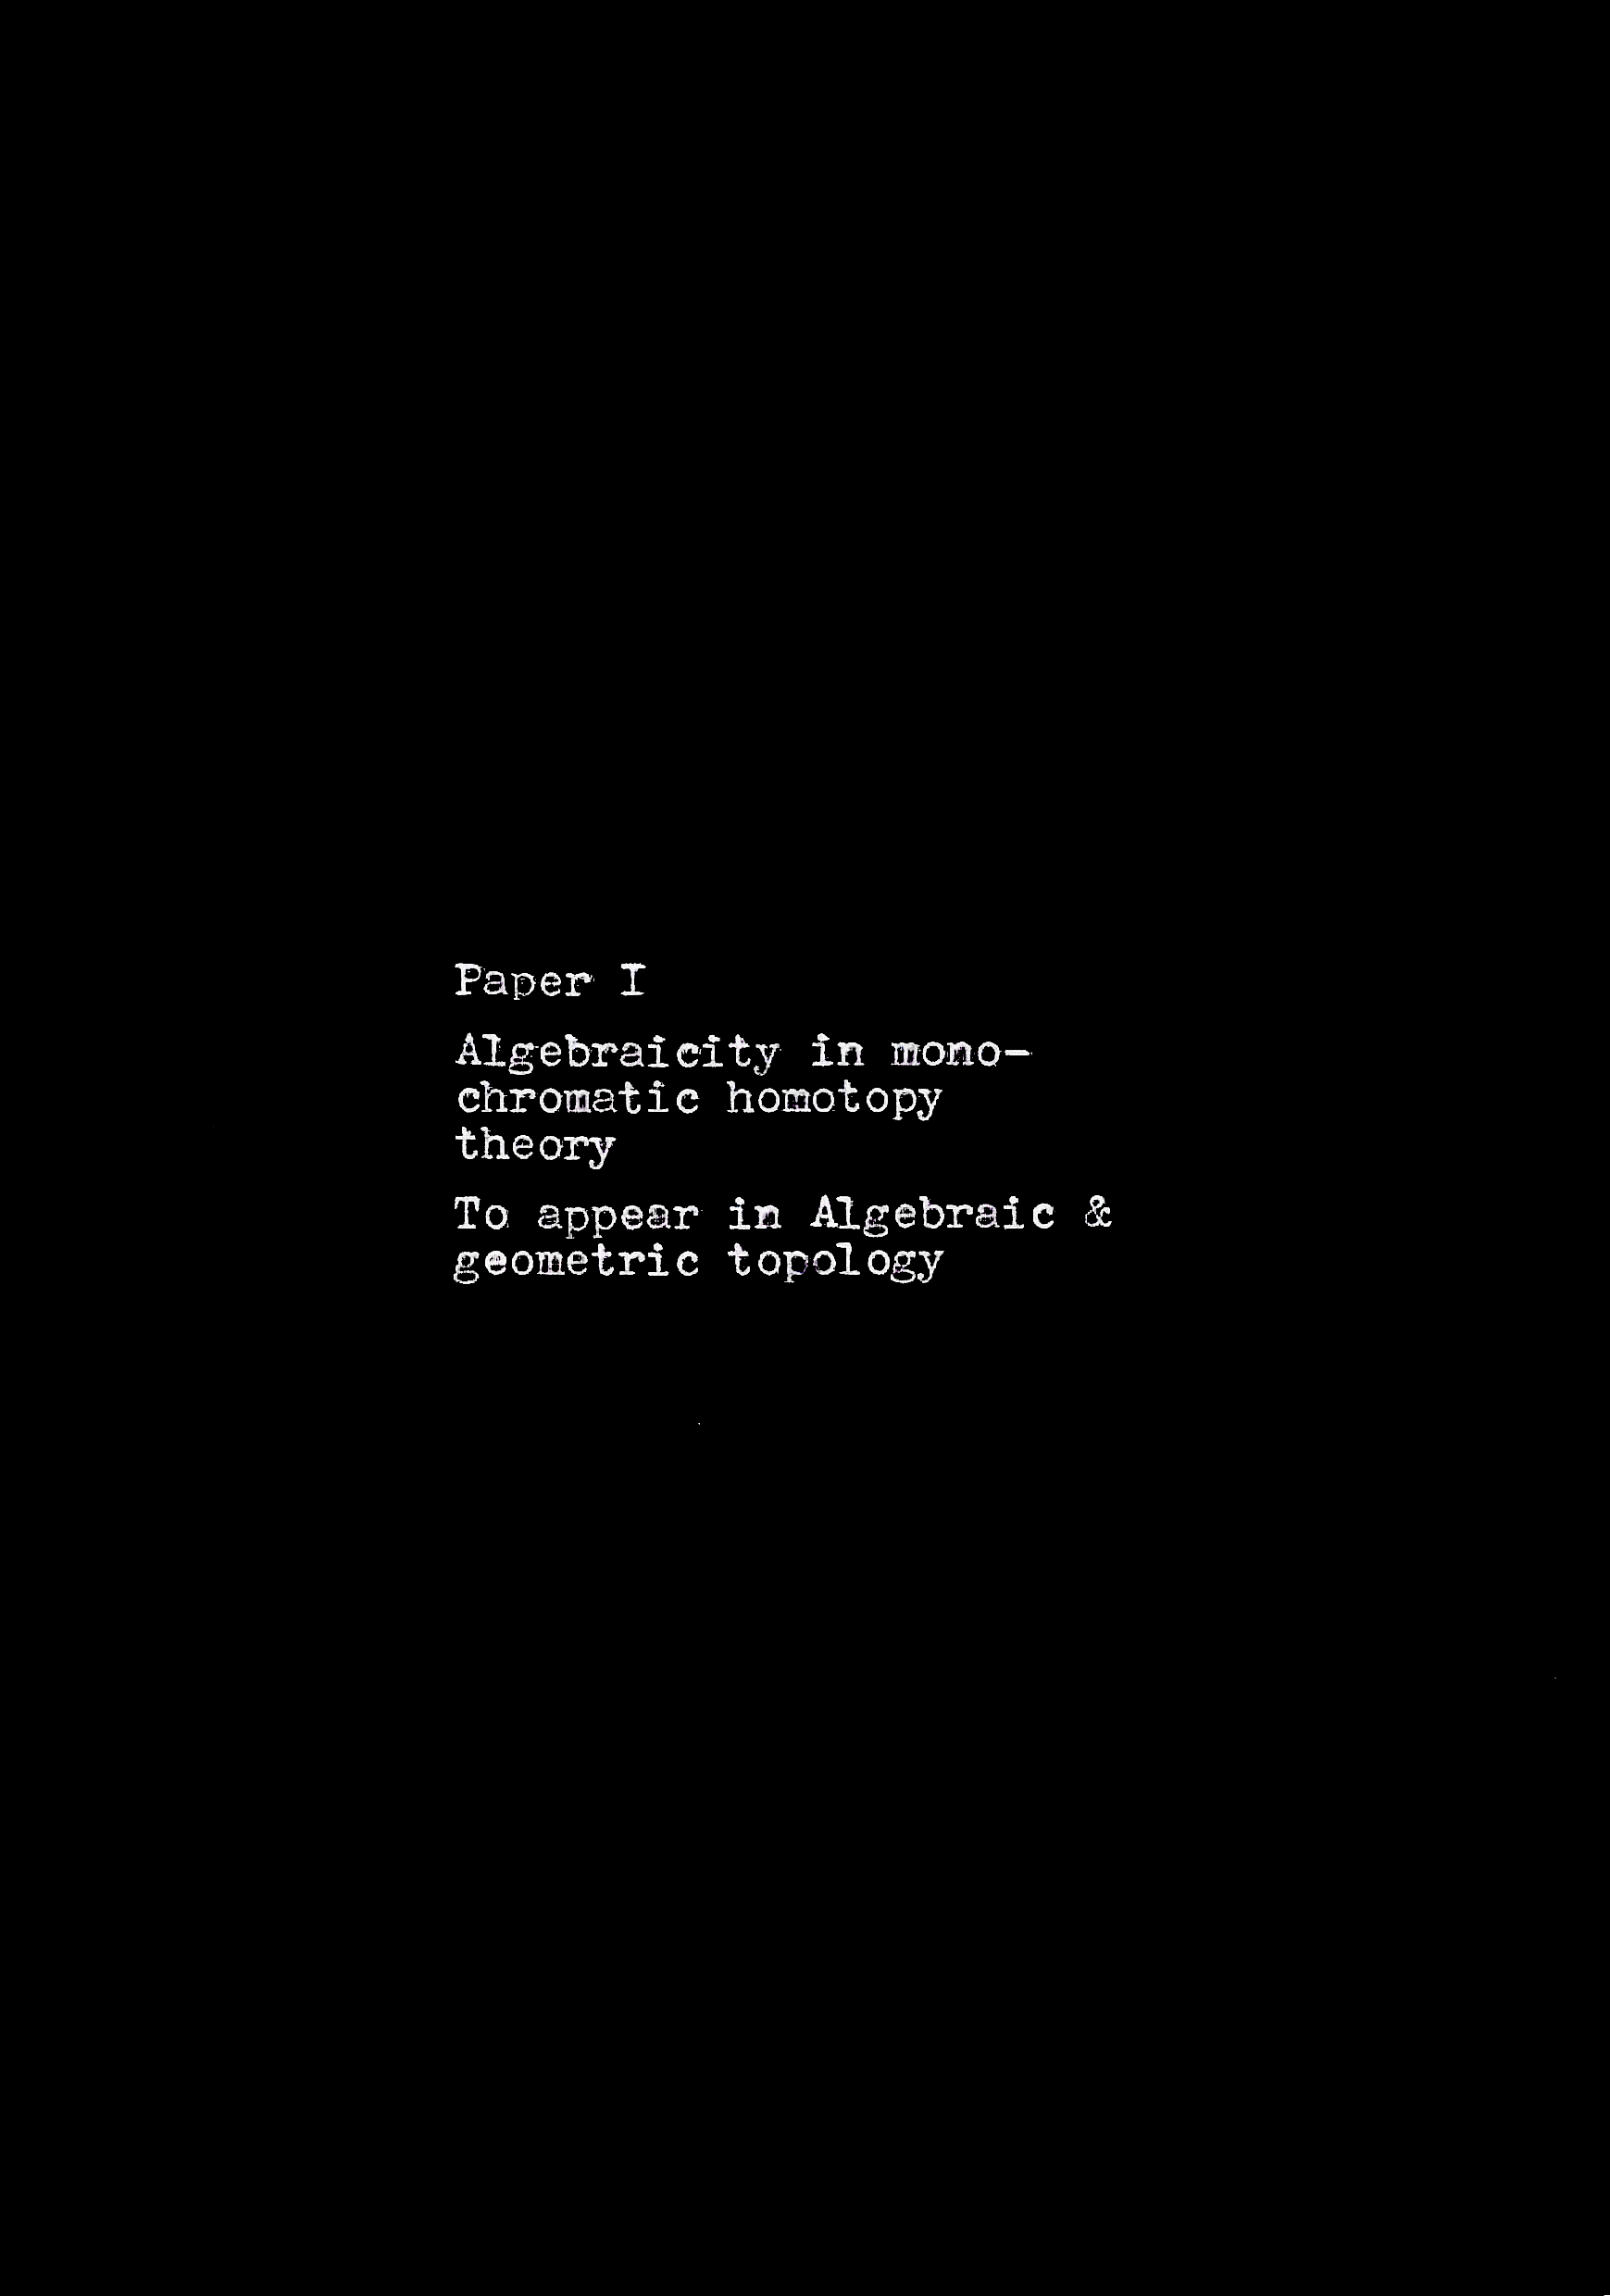
\includegraphics[%
clip,
width=1.05\paperwidth,
height=1.05\paperheight
]{chaptertitles/paper1b.png}};

\clearpage


\newpage
\tikz[remember picture,overlay]\node[opacity=1,inner sep=0pt] at (current page.center)%
{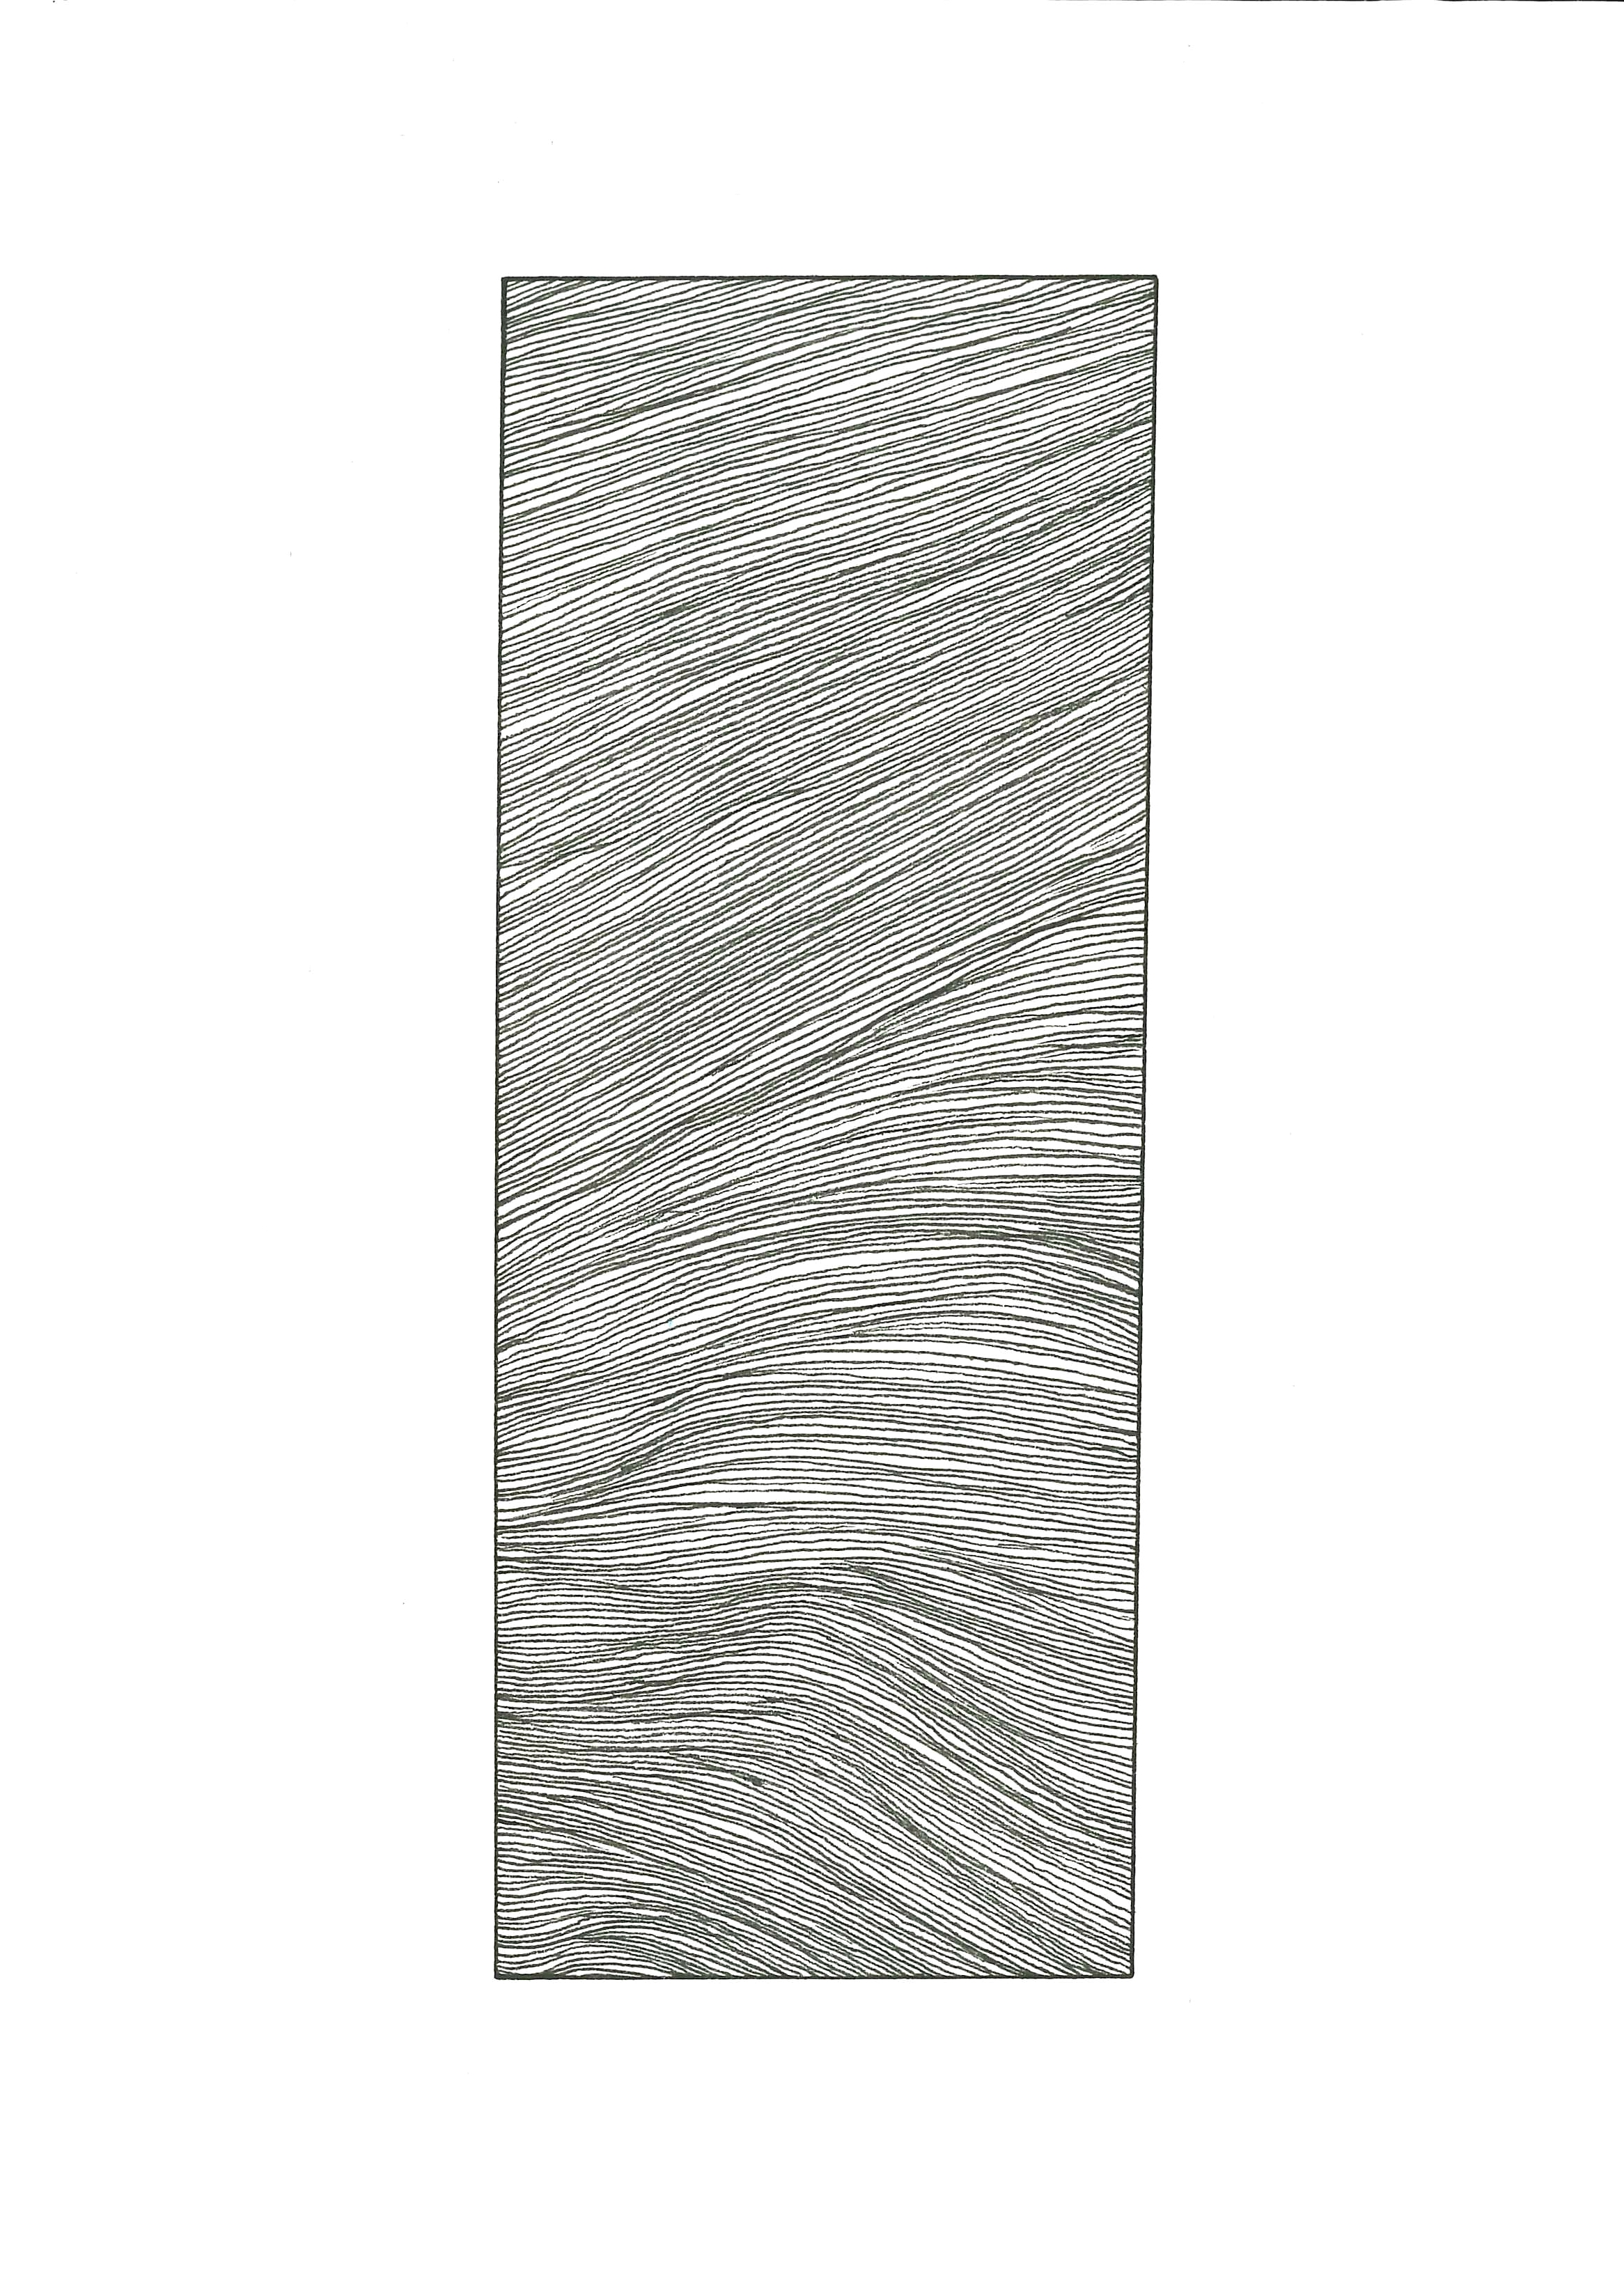
\includegraphics[%
clip,
width=1.05\paperwidth,
height=1.05\paperheight
]{chaptertitles/drawing1.jpeg}};

\clearpage


%\subsection*{Description}



\vspace*{2em}

{\par\centering {\Large \textbf{Description:}}\par}
\vspace{-2em}
\rule[-11pt]{\textwidth}{1pt}
\rule{\textwidth}{0.5pt}
    
The main result of the first paper concerns the behaviour of a class of objects when a parameter is increased. At low values the objects act in a very topological manner---which in spirit acts like fluidity, movement, deformation. Increasing the parameter makes the objects behave more and more algebraically, which is more rigid, less fluid, more staccato, more mechanical. Above a certain threshold, the behaviour of the objects is completely algebraic, which is depicted using only straight lines, while the topological behaviour at lower values is depicted with more flowing curved lines. 

\rule{\textwidth}{0.5pt}
\rule[11pt]{\textwidth}{1pt}


\newpage

\thispagestyle{plain}

\section*{}
\addcontentsline{toc}{section}{Limerick I}



\vspace*{7cm}

\begin{verse}
    \hspace{8em}A prime and a height at their station, \\
    \vspace{5pt}
    \hspace{8em}declares their latest dictation: \\
    \vspace{5pt}
    \hspace{8em}The chromatic tower, \\
    \vspace{5pt}
    \hspace{8em}is in increasing power, \\
    \vspace{5pt}
    \hspace{8em}described by algebraic information.

    %\hspace{\fill}-- Torgeir Aambø
\end{verse}










\newpage


\vspace*{2em}

{\par\centering {\Large \textbf{Abstract:}}\par}
\vspace{-2em}
\rule[-11pt]{\textwidth}{1pt}
\rule{\textwidth}{0.5pt}
    
Using Patchkoria--Pstr{\k a}gowski's version of Franke's algebraicity theorem, we prove that the category of $\Kpn$-local spectra is exotically equivalent to the category of derived $I_n$-complete periodic comodules over the Adams Hopf algebroid $(E_*, E_*E)$ for large primes. This gives a finite prime result analogous to the asymptotic algebraicity for $\SpKpn$ of Barthel--Schlank--Stapleton. 

\rule{\textwidth}{0.5pt}
\rule[11pt]{\textwidth}{1pt}

{\setstretch{0.5}
\printcontents[chapters]{p}{1}{}
}
\vspace{\fill}






\section{Introduction}
\label{ch1:sec:introduction}

The central idea in chromatic homotopy theory is to study the symmetric monoidal stable $\infty$-category of spectra, $\Sp$, via its smaller building blocks. These are the categories $\Sp\np$ and $\SpKpn$ of $\Enp$-local and $\Kpn$-local spectra, where $E=\Enp$ is Morava $E$-theory, and $\Kpn$ is Morava $K$-theory---see for example \cite{hovey-strickland_99}. These categories depend on a prime $p$ and an integer $n$, called the chromatic height. For a fixed height $n$, increasing the prime $p$ makes both categories behave more algebraically. This manifests itself, for example, in the $E$-Adams spectral sequence of signature
\[E^{s,t}_2 (L\np\S) = \Ext_{E_*E}^{s,t}(E_*,E_*)\Longrightarrow \pi_{t-s} L\np\S\]
computing the homotopy groups of the $E$-local sphere. By the smash product theorem of Ravenel, see \cite[7.5.6]{ravenel_92}, this spectral sequence has a horizontal vanishing line at a finite page. If $p>n+1$, this vanishing line appears already on the second page, where the information is completely described by the homological algebra of $\ComodE$---the Grothendieck abelian category of comodules over the Hopf algebroid $(E_*, E_*E)$. 

Increasing the prime $p$ correspondingly increases the distance between objects appearing in the $E$-Adams spectral sequence. When $2p-2$ exceeds $n^2+n$, there is no longer room for any differentials, and the  spectral sequence in fact collapses to an isomorphism
\[\pi_* L\np\S\cong \Ext^{*,*}\EE(E_*, E_*),\]
for degree reasons. In other words, the homotopy groups are completely algebraic in this range. 

A natural question to ask is whether this collapse is a feature solely of the $E$-Adams spectral sequence or if it is a feature of the category $\Sp\np$. More precisely, is the entire category of $E$-local spectra algebraic, in the sense that it is equivalent to a derived category of an abelian category, whenever $2p-2>n^2+n$? What about the category of $\Kpn$-local spectra?

At height $n=0$, both categories $\Sp\np$ and $\SpKpn$ is the category of rational spectra $\Sp_\Q$, which can be seen to be equivalent to the derived $\infty$-category of rational vector spaces, but at positive heights $n>0$, there can never be an equivalence of $\infty$-categories 
\[\Sp\np \simeq \Der(\A) \text{ or } \SpKpn \simeq \Der(\A).\]

However, in \cite{bousfield_1985} Bousfield showed that for $p>2$ and $n=1$, that there is an equivalence of homotopy categories
\[h \Sp_{1,p}\simeq h \Fr_{1,p},\]
where $\Fr\np$ is a certain derived $\infty$-category of twisted comodules over $(E_*, E_*E)$. As this cannot be lifted to an equivalence of $\infty$-categories, it is sometimes referred to as an \emph{exotic} equivalence. 

Franke expanded upon this in \cite{franke_96} by conjecturing---and attempting to prove---that for $2p-2 > n^2+n$ there should be an equivalence of homotopy categories
\[h \Sp\np\simeq h \Fr\np.\]
Unfortunately, a subtle error was discovered in the proof by Patchkoria in \cite{patchkoria_2013}, but the result was recovered in \cite{pstragowski_2021} with a slightly worse bound: $2p-2>2n^2+2n$. Pstr\a{}gowski also proved that this equivalence gets ``stronger'' the larger the prime, where we not only get an equivalence of categories but an equivalence of $k$-categories 
\[h_k \Sp\np\simeq h_k \Fr\np,\]
for $k=2p-2-2n^2-2n$. Here $h_k \C$ denotes taking the homotopy $k$-category, given by $(k-1)$-truncating the mapping spaces in $\C$. At $k=1$, this gives the classical situation of taking the homotopy category $h\C$. Using and developing a more general machinery, Pstr\a{}gowski and Patchkoria proved in \cite{patchkoria-pstragowski_2021} that the above equivalence holds in Franke's conjectured bound:
\[2p-2>n^2+n.\] 

The current belief is that these bounds are optimal. We know this to be true at the prime $2$, as Roitzheim proved in \cite{roitzheim_07} that the category $\Sp_{1,2}$ is \emph{rigid}, in the sense that any equivalence of homotopy categories $h\Sp_{1,2} \simeq h\C$ lifts to an equivalence $\Sp_{1,2}\simeq \C$. The $K_p(n)$-local analogue of Roitzheim's result also holds, as Ishak proved in \cite{ishak_19} that $\Sp_{K_2(1)}$ is rigid as well. Hence, exotic equivalences for $\Sp\np$ or $\SpKpn$ can only exist at primes that are large compared to the height. 

The above results imply that increasing the prime $p$ decreases how destructive the $k$-truncation of the mapping spaces needs to be. In the limit $p\rightarrow \infty$, we might expect that there is no need to truncate at all, giving an equivalence of $\infty$-categories. But, there needs to be an appropriate notion of what ``going to the infinite prime'' should be. In \cite{barthel-schlank-stapleton_2020}, the authors use a notion of ultraproducts over a non-principal ultrafilter of primes, $\mathcal{F}$, to formalize this limiting process. They use this to prove the existence of a symmetric monoidal equivalence of $\infty$-categories
\[\prod_{\mathcal{F}}\Sp\np \simeq \prod_{\mathcal{F}}\Fr\np.\] 
Expanding on their work, Barthel, Schlank, and Stapleton proved in \cite{barthel-schlank-stapleton_2021} a $\Kpn$-local version of the above result. More precisely, they show that there is a symmetric monoidal equivalence of $\infty$-categories
\[\prod_{\mathcal{F}}\SpKpn \simeq \prod_{\mathcal{F}}\Frc,\]
where the right-hand side consists of derived complete twisted comodules for the naturally occurring Landweber ideal $I_n\subseteq E_*$. 

\textbf{Statement of results:} We can summarize the most general of the above algebraicity results in the following table,
\vspace{-10pt}
\begin{table}[h]
    \centering
    \begin{tabular}{c|ccc}
        & $p<\infty $ & $p\rightarrow \infty$ \\
        \hline 
        $\Sp\np$& \cite{patchkoria-pstragowski_2021} & \cite{barthel-schlank-stapleton_2020} \\
        $\SpKpn$ &  & \cite{barthel-schlank-stapleton_2021} 
    \end{tabular}
\end{table}

A natural question arises: Is there a finite prime exotic algebraicity for $\SpKpn$? The goal of this paper is to give an affirmative answer. More precisely, we prove the following. 

\begin{introthm}[\cref{ch1:thm:main-spectra-dual}]
    \label{ch1:thm:A}
    Let $p$ be a prime and $n$ a non-negative integer. If $k=2p-2-n^2-n>0$, then there is an equivalence of homotopy $k$-categories 
    \[h_k \SpKpn\simeq h_k \Frc.\]
    In other words, $K_p(n)$-local spectra are exotically algebraic at large primes. 
\end{introthm}

The available tools for proving such a statement require an abelian category with enough injective objects admitting lifts to a stable $\infty$-category. In lack of such a well-behaved abelian approximation for $\SpKpn$, we take inspiration from \cite{barthel-schlank-stapleton_2021} and instead use the dual category $\M\np$ of monochromatic spectra, which we show has the needed properties. \cref{ch1:thm:A} will then follow from the following result. 

\begin{introthm}[\cref{ch1:thm:main-spectra}]
    \label{ch1:thm:B}
    Let $p$ be a prime and $n$ a non-negative integer. If $k=2p-2-n^2-n>0$,  then there is an equivalence 
    \[h_k \M\np\simeq h_k \Fr\np\Int\]
    of homotopy $k$-categories.
\end{introthm}

In order to prove \cref{ch1:thm:B}, we first prove the analogous statement for monochromatic $E$-modules. 
    
\begin{introthm}[\cref{ch1:thm:main-modules}]
    \label{ch1:thm:C}
    Let $p$ be a prime and $n$ a non-negative integer. If $k=2p-2-n>0$,  then there is an equivalence
    \[h_k \Modt\simeq h_k \Dper(\modt)\]
    of homotopy $k$-categories.
\end{introthm}


\textbf{Overview of the paper:} \cref{ch1:sec:introduction} introduces local duality, and the proposed exotic algebraic model using periodic chain complexes of torsion comodules. \cref{ch1:sec:exotic-algebraic-models} focuses on Franke's algebraicity theorem. Most of the new results of the paper are presented in \cref{ch1:ssec:algebraicity-modules} and \cref{ch1:ssec:algebraicity-spectra}, where we prove \cref{ch1:thm:A}, \cref{ch1:thm:B} and \cref{ch1:thm:C}. In \cref{ch1:app:barr-beck} we prove that Barr--Beck adjunctions interact well with local duality, which is used to prove that periodization, torsion and taking the derived category all commute. 


\textbf{Acknowledgements:} We want to thank Drew Heard, Irakli Patchkoria and Marius Nielsen for helpful conversations and for proof-reading the paper. We also want to thank Piotr Pstr\a{}gowski for finding a mistake in the proof of a previous version of \cref{ch1:lm:cohomological-dimension-torsion-comodules}, and the anonymous referee for helpful and constructive comments. Lastly, we want to thank the University of Copenhagen for their hospitality while writing most of this paper. This work forms a part of the author's thesis, partially supported by grant number TMS2020TMT02 from the Trond Mohn Foundation. 

\section{The algebraic model}

The goal of this section is to set up the necessary background material that will be used throughout the paper. We use these to construct convenient algebraic approximations of categories arising from chromatic homotopy theory. 

\subsection*{Some conventions}

We freely use the language of $\infty$-categories, as developed by Joyal \cite{joyal_02} and Lurie \cite{lurie_09, Lurie_HA}. Even though we are dealing with both classical $1$-categories and $\infty$-categories in this paper, we will sometimes refer to them both as \emph{categories}, hoping that the prefix is clear from the context. 

We denote by $\PrLs$ the $\infty$-category of presentable stable $\infty$-categories and colimit preserving functors. Together with the Lurie tensor product, it is a symmetric monoidal $\infty$-category. The category of commutative algebras $\CAlg(\PrLs)$ is then the category of presentable stable $\infty$-categories with a symmetric monoidal structure commuting with colimits separately in each variable. 

Let $\C, \D\in \CAlg(\PrLs)$. A localization is a functor $f\colon \C\to \D$ with a fully faithful right adjoint $i$. We denote the composite by $L= i\circ f$. The adjoint $i$ identifies $\D$ with a full subcategory of $\C$, which we denote by $\C_L$. We then view $L$ as a functor $L\colon \C\to\C_L$, that is left adjoint to the inclusion, and by abuse of notation also call these localizations. 










%%%%%%%%%%%%%%%%%%%%%%%%%%%%%%%%%%%%%%%%%%%%%%%%%%%%%%%%%%%%%%%%%%%%%%%%%%%%%%









\subsection{Local duality}

The theory of abstract local duality, proved in \cite{hovey-palmiery-strickland_97} and generalized to the $\infty$-categorical setting in \cite{barthel-heard-valenzuela_2018} will be important for the entire paper. In particular, it is the technology that will allow us to translate \cref{ch1:thm:B} into \cref{ch1:thm:A}. 

\begin{definition}
    \label{ch1:def:local-duality-context}
    \index{Local duality!Context}
    A pair $(\C, \K)$, where $\C\in \CAlg(\PrLs)$ is compactly generated by dualizable objects, and $\K$ is a subset of compact objects, is called a \emph{local duality context}.
\end{definition}

\begin{construction}
    \index{Local duality!Torsion objects}
    \index{Local duality!Local objects}
    \index{Local duality!Complete object}
    \index{Right orthogonal complement}
    Let $(\C, \K)$ be a local duality context. We define $\C\Ktors$ to be the localizing tensor ideal generated by $\K$, denoted $\Loc^\otimes_\C(\K)$. Further we define $\C\Kloc$ to be the right orthogonal complement $(\C\Ktors)^\perp$, i.e., the full subcategory consisting of objects $C\in \C$ such that $\Hom_\C(T,C)\simeq 0$ for all $T\in \C\Ktors$. Similarly, define $\C\Kcomp$ to be the right orthogonal complement of $\C\Kloc$, i.e. $\C\Kcomp= (\C\Kloc)^\perp$. These full subcategories are respectively called the $\K$-torsion, $\K$-local and $\K$-complete objects in $\C$. We have inclusions into $\C$, denoted $i_{\K-\mathrm{tors}}$, $i_{\K-\mathrm{loc}}$ and $i_{\K-\mathrm{comp}}$ respectively. 
    
    By the adjoint functor theorem, \cite[5.5.2.9]{lurie_09}, the inclusions $i_{\K-\mathrm{loc}}$ and $i_{\K-\mathrm{comp}}$ have left adjoints $L_\K$ and $\Lambda_\K$ respectively, while $i_{\K-\mathrm{tors}}$ and $i_{\K-\mathrm{loc}}$ have right adjoints $\Gamma_\K$ and $V_\K$ respectively. These are then, by definition, localizations and colocalizations. Since the torsion, local and complete objects are ideals, these localizations and colocalizations are compatible with the symmetric monoidal structure of $\C$, in the sense of \cite[2.2.1.7]{Lurie_HA}. In particular, by \cite[2.2.1.9]{Lurie_HA} we get unique induced symmetric monoidal structures such that $L_\K$, $\Lambda_\K$, $\Gamma_\K$ and $V_\K$ are symmetric monoidal functors. 

    For any $X\in \C$, these functors assemble into two cofiber sequences:
    $$\Gamma_\K X \longrightarrow X \longrightarrow L_\K X \quad \text{and}\quad V_\K X \longrightarrow X \longrightarrow \Lambda_\K X.$$
    Note also that these functors only depend on the localizing subcategory $\C\Ktors$, not on the particular choice of generators $\K$. Thus, when the set $\K$ is clear from the context, we often omit it as a subscript when writing the functors. 
\end{construction}

The following theorem is a slightly restricted version of the abstract local duality theorem of \cite[3.3.5]{hovey-palmiery-strickland_97} and \cite[2.21]{barthel-heard-valenzuela_2018}.  

\begin{theorem}
    \label{ch1:thm:local-duality}
    \index{Local duality!Theorem}
    Let $(\C, \K)$ be a local duality context. Then
    \begin{enumerate}
        \item the functors $\Gamma$ and $L$ are smashing, meaning that there are natural equivalences
        \[\Gamma X\simeq X\otimes \Gamma \1 \text{ and } LX\simeq X\otimes L\1,\]
        \item the functors $\Lambda$ and $V$ are cosmashing, meaning there are natural equivalences
        \[\Lambda X\simeq \iHom(\Gamma \1,X) \text{ and } VX\simeq \iHom(L\1, X),\] 
        and
        \item the functors 
        \[\Gamma\colon \C\Kcomp\longrightarrow \C\Kcomp \text{ and } \Lambda\colon \C\Ktors\longrightarrow \C\Kcomp\] 
        are mutually inverse symmetric monoidal equivalences of categories.
    \end{enumerate}
    This can be summarized by the following diagram of adjoints
    \begin{center}
        \begin{tikzcd}
                & {\C\Kloc} \\
                & {\C} \\
                {\C\Ktors} && {\C\Kcomp}
                \arrow["L", xshift=-4pt, from=2-2, to=1-2]
                \arrow[from=1-2, to=2-2]
                \arrow["V", xshift=4pt, from=2-2, to=1-2, swap]

                \arrow["\Lambda", yshift=2pt, xshift=2pt, from=2-2, to=3-3]
                \arrow[yshift=-2pt, xshift=0pt, from=3-3, to=2-2]

                \arrow["\Gamma", yshift=-2pt, xshift=0pt, from=2-2, to=3-1]
                \arrow[yshift=2pt, xshift=-2pt, from=3-1, to=2-2]
                
                \arrow[bend left=35, dashed, from=3-1, to=1-2]
                \arrow[bend left=35, dashed, from=1-2, to=3-3]

                \arrow["\simeq"', swap, from=3-1, to=3-3]
        \end{tikzcd}    
    \end{center}
\end{theorem}

\begin{remark}
    \label{ch1:rm:monoidal-structure-in-local-duality}
    \cref{ch1:thm:local-duality} implies, in particular, that the symmetric monoidal structure induced by the localization $L$ and the colocalization $\Gamma$ is just the symmetric monoidal structure on $\C$ restricted to the full subcategories. This is not the case for $\C\Kcomp$, where the symmetric monoidal structure is given by $\Lambda(-\otimes_\C-)$. The functor $V$ also induces a symmetric monoidal structure on $\C\Kloc$, but this coincides with the one induced by $L$, due to their associated endofunctors on $\C$ defining an adjoint symmetric monoidal monad-comonad pair. Note that we will not need or focus on the functor $V$, hence it will be omitted from the local duality diagrams for the rest of the paper. 
\end{remark}

\begin{addendum}
    An alternative proof of local duality, using a version of Positselski's co/contra correspondence in symmetric monoidal stable $\infty$-categories, can be found in \cref{ch2}---more specifically \cref{ch2:thm:local-duality-co-contra}. 
\end{addendum}

We have two main examples of interest for this paper. 

\begin{example}
    \label{ch1:ex:local-duality-comod}
    \index{Local duality!Hopf algebroid}
    Let $(A,\Psi)$ be an Adams type Hopf algebroid, for example the Hopf algebroid $(R_*, R_*R)$ for an Adams type ring spectrum $R$---see \cite[A.1]{ravenel_86} and \cite{hovey_04} for details. Denote by $\Der(\Psi)$ the derived $\infty$-category associated to the symmetric monoidal Grothendieck abelian category $\Comod_\Psi$. This is defined using the model structure from \cite{barnes-roitzheim_2011}. If $I\subseteq A$ is a finitely generated invariant regular ideal, then $(\Der(\Psi), A/I)$ is a local duality context, with associated local duality diagram
    \begin{center}
        \begin{tikzcd}
            & {\Der(\Psi)\Iloc} \\
            & {\Der(\Psi)} \\
            {\Der(\Psi)\Itors} && {\Der(\Psi)\Icomp}
            \arrow["L_I^\Psi", xshift=-2pt, from=2-2, to=1-2]
            \arrow[xshift=2pt, from=1-2, to=2-2]

            \arrow["\Delta_I^\Psi", yshift=2pt, xshift=2pt, from=2-2, to=3-3]
            \arrow[yshift=-2pt, xshift=0pt, from=3-3, to=2-2]

            \arrow["\Gamma^\Psi_I", yshift=-2pt, xshift=0pt, from=2-2, to=3-1]
            \arrow[yshift=2pt, xshift=-2pt, from=3-1, to=2-2]

            \arrow[bend left=35, dashed, from=3-1, to=1-2]
            \arrow[bend left=35, dashed, from=1-2, to=3-3]

            \arrow["\simeq"', swap, from=3-1, to=3-3]
        \end{tikzcd}    
    \end{center}
\end{example}

In \cref{ch1:ssec:the-algebraic-model} we compare $\Der(\Psi)\Itors$ to a more concrete category: the derived category of $I$-power torsion comodules.  

The following example comes from chromatic homotopy theory. For a good introduction, see \cite{barthel-beaudry_19}. 

\begin{example}
    \label{ch1:ex:local-duality-chromatic}
    \index{Local duality!Chromatic}
    Let $E$ denote Morava $E$-theory at prime $p$ and height $n$. If $F(n)$ is a finite type $n$ spectrum, then the pair $(\Sp\np, L\np F(n))$ is a local duality context. The corresponding diagram can be recognized as
    \begin{center}
        \begin{tikzcd}
                & {\Sp_{n-1,p}} \\
                & {\Sp\np} \\
                {\M\np} && {\SpKpn}
                \arrow["L_{n-1,p}", xshift=-2pt, from=2-2, to=1-2]
                \arrow[xshift=2pt, from=1-2, to=2-2]

                \arrow["L_\Kpn", yshift=2pt, xshift=2pt, from=2-2, to=3-3]
                \arrow[yshift=-2pt, xshift=0pt, from=3-3, to=2-2]

                \arrow["M\np", yshift=-2pt, xshift=0pt, from=2-2, to=3-1]
                \arrow[yshift=2pt, xshift=-2pt, from=3-1, to=2-2]

                \arrow[bend left=35, dashed, from=3-1, to=1-2]
                \arrow[bend left=35, dashed, from=1-2, to=3-3]

                \arrow["\simeq"', swap, from=3-1, to=3-3]
        \end{tikzcd}    
    \end{center}
    where $\M\np$ is the height $n$ monochromatic category\index{Monochromatic spectra} and $\SpKpn$ is the category of spectra localized at height $n$ Morava $K$-theory $\Kpn$\index{Morava $K$-theory}. The functor $L_{n-1,p}$ is the Bousfield localization at $E_{n-1,p}$, while $L_{\Kpn}$ is the Bousfield localization at $\Kpn$, see \cite{bousfield_1979_localization}. The local duality then exhibits the classical equivalence 
    \[\M\np\simeq \SpKpn,\] 
    see \cite[6.19]{hovey-strickland_99}. 
\end{example}

\begin{remark}
    \label{ch1:rm:local-duality-modules}
    There is also a version of this local duality diagram for modules over $E$, see \cite[4.2, 5.1]{greenlees-may_1995}, or alternatively \cite[3.7]{barthel-heard-valenzuela_2018} for a version more similar to the above. This gives equivalences 
    \[\M\np\ModE\simeq \Modt\simeq \Modc\simeq L_{\Kpn}\ModE,\]
    where $I_n$ is the Landweber ideal $(p,v_1, \ldots, v_{n-1})\subseteq E_*$.
\end{remark}

\begin{addendum}
    We have expanded upon the theory of local duality, as well as comodules over a Hopf algebroid and monochromatic spectra in \cref{ch0:ssec:local-duality}, \cref{ch0:ssec:hopf-algebroids-and-their-comodules} and \cref{ch0:sssec:monochromatic-duality} respectively. 
\end{addendum}







%%%%%%%%%%%%%%%%%%%%%%%%%%%%%%%%%%%%%%%%%%%%%%%%%%%%%%%%%%%%%%%%%%%%%%%%%%%%%%










\subsection{The periodic derived torsion category}
\label{ch1:ssec:the-algebraic-model}

In this section we identify the category $\Der(\Psi)\Itors$---as obtained in \cref{ch1:ex:local-duality-comod}---as the derived category of $I$-power torsion comodules. We also modify the category to exhibit some needed periodicity. 

\begin{definition}
    \label{ch1:def:I-power-torsion-comodule}
    \index{I-power torsion!Comodule}
    Let $(A,\Psi)$ be an Adams Hopf algebroid and $I\subseteq A$ a regular invariant ideal. The\emph{$I$-power torsion} of a comodule $M$ is defined as 
    $$T_I^\Psi M = \{x\in M \mid I^k x = 0 \text{ for some } k\in \N\}.$$
    We say a comodule $M$ is \emph{$I$-power torsion} if the natural comparison map $T_I^\Psi M\longrightarrow M$ is an equivalence. 
\end{definition}

\begin{remark}
    \label{ch1:rm:torsion-iff-underlying-is-torsion}
    One can similarly define $I$-power torsion $A$-modules. If $(A,\Psi)$ is an Adams Hopf algebroid, then a $\Psi$-comodule $M$ is $I$-power torsion if and only if its underlying module is $I$-power torsion, see \cite[5.7]{barthel-heard-valenzuela_2018}. 
\end{remark}

\begin{remark}
    \label{ch1:rm:torsion-comodules-grothendieck-monoidal}
    By \cite[5.10]{barthel-heard-valenzuela_2018} the full subcategory of $I$-power torsion comodules, which we denote $\Comod_\Psi\Itors$, is a Grothendieck abelian category. It also inherits a symmetric monoidal structure from $\Comod_\Psi$. 
\end{remark}

The following technical lemma will be needed later. 

\begin{lemma}
    \label{ch1:lm:torsion-comodules-generated-by-compacts}
    Let $(A,\Psi)$ be an Adams Hopf algebroid, where $A$ is noetherian and $I\subseteq A$ a regular invariant ideal. Then $\Comod_\Psi\Itors$ is generated under filtered colimits by the compact $I$-power torsion comodules. 
\end{lemma}
\begin{proof}
    By \cite[3.4]{barthel-heard-valenzuela_2020} $\Comod_\Psi\Itors$ is generated by the set 
    $$\Tors_\Psi^{fp}:=\{G\otimes A/I^k \mid G \in \Comod_\Psi^{fp}, k\geq 1\},$$
    where $\Comod_\Psi^{fp}$ is the full subcategory of dualizable $\Psi$-comodules. Since $I$ is finitely generated and regular, $A/I^k$ is finitely presented as an $A$-module, hence it is compact in $\Comod_\Psi$ by \cite[1.4.2]{hovey_04}, and also in $\Comod_\Psi\Itors$, as colimits are computed in $\Comod_\Psi$. Because $A$ was assumed to be noetherian, being finitely generated and finitely presented coincide. The tensor product of finitely generated modules is finitely generated, hence any element in $\Tors_\Psi^{fp}$ is compact. 
\end{proof}

\begin{remark}
    The assumption that the ring $A$ is noetherian can most likely be removed, but it makes no difference to the results in this paper.  
\end{remark}

\begin{notation}
    Since $\Comod_\Psi\Itors$ is Grothendieck abelian we have an associated derived stable $\infty$-category $\Der(\Comod_\Psi\Itors)$ which we denote simply by $\Der(\Psi\Itors)$.
\end{notation}

We e can now compare the torsion category obtained from local duality and the derived category of $I$-power torsion comodules. 

\begin{lemma}[{\cite[3.7(2)]{barthel-heard-valenzuela_2020}}]
    \label{ch1:lm:derived-torsion-if-homology-torsion}
    Let $(A,\Psi)$ be an Adams Hopf algebroid and $I\subseteq A$ a regular invariant ideal. There is an equivalence of categories 
    $$\Der(\Psi)\Itors\simeq \Der(\Psi\Itors).$$ 
    Furthermore, an object $M\in \Der(\Psi)$ is $I$-torsion if and only if the homology groups $H_* M$ are $I$-power torsion $\Psi$-comodules.
\end{lemma}

\begin{addendum}
    We can construct an alternative proof of the above result using the theory developed in \cref{ch3}. In particular, the two categories $\Der(\Psi)\Itors$ and $\Der(\Psi\Itors)$ are both $\pi$-stable localizing ideals of $\Der(\Psi)$ with the same heart $\Comod_\Psi\Itors$, which by \cref{ch3:thm:premain} means they have to be equivalent. 
\end{addendum}

In order to state both the general algebraicity machinery of \cite{patchkoria-pstragowski_2021} and our results, we need the respective derived categories to exhibit the periodic nature of the spectra we are interested in. This is done via the periodic derived category. There are several ways to constructing this, but we follow \cite{franke_96} in spirit, using periodic chain complexes. 

\begin{definition}
    \label{ch1:def:periodic-chain-complex}
    \index{Periodic!Chain complex}
    Let $\A$ be an abelian category with a local grading, i.e., an auto-equivalence $T\colon \A\to\A$, and denote $[1]$ the shift functor on the category of chain complexes $\Ch(\A)$ in $\A$. A chain complex $C\in \Ch(\A)$ is called \emph{periodic} if there is an isomorphism $\phi\colon C[1]\longrightarrow TC$. The full subcategory of periodic chain complexes is denoted by $\Chp(\A)$. 
\end{definition}

\begin{definition}
    \index{Periodization}
    The forgetful functor $\Chp(\A)\longrightarrow \Ch(\A)$ has a left adjoint $P$, called the \emph{periodization}. 
\end{definition}

\begin{definition}
    \label{ch1:def:periodic-derived-category}
    \index{Periodic!Derived category}
    If $\A$ is a locally graded abelian category, then the \emph{periodic derived category} of $\A$, denoted $\Dper(\A)$, is defined to be the $\infty$-category obtained by localizing $\Chp(\A)$ at the quasi-isomorphism. It is a stable $\infty$-category by \cite[7.8]{patchkoria-pstragowski_2021}. 
\end{definition}

\begin{remark}
    \label{ch1:rm:periodic-derived-as-modules}
    \index{Periodic!Unit}
    If $\A$ is a symmetric monoidal category with unit $\1$, then $P\1$ is a commutative ring object called the \emph{periodic unit}. By \cite[2.3]{barnes-roitzheim_2011} the category of periodic chain complexes $\Chp(\A)$ is equivalent to $\Mod_{P\1}(\Ch(\A))$. This descends also to the derived categories, giving an equivalence 
    $$\Dper(\A)\simeq \Mod_{P\1}(\Der(\A)),$$
    see for example \cite[3.7]{pstragowski_2021}. 
\end{remark}

We will also need local duality  for the periodic derived category associated to a Hopf algebroid. 

\begin{construction}
    \label{ch1:const:periodic-derived-local-duality}
    Let $(A, \Psi)$ be an Adams type (graded) Hopf algebroid. Then the shift functor $[1]\colon \Comod_\Psi\longrightarrow \Comod_\Psi$
    defined by $(TM)_k = M_{k-1}$ is a local grading on $\Comod_\Psi$. Denote the corresponding periodic derived category by $\Dper(\Psi)$. The pair $(\Dper(\Psi), P(A/I))$ is a local duality context with associated local duality diagram
    \begin{center}
    \begin{tikzcd}
        & {\Dper(\Psi)\Iloc} \\
        & {\Dper(\Psi)} \\
        {\Dper(\Psi)\Itors} && {\Dper(\Psi)\Icomp}
        \arrow["L_I^\Psi", xshift=-2pt, from=2-2, to=1-2]
        \arrow[xshift=2pt, from=1-2, to=2-2]

        \arrow["\Lambda_I^\Psi", yshift=2pt, xshift=2pt, from=2-2, to=3-3]
        \arrow[yshift=-2pt, xshift=0pt, from=3-3, to=2-2]

        \arrow["\Gamma^\Psi_I", yshift=-2pt, xshift=0pt, from=2-2, to=3-1]
        \arrow[yshift=2pt, xshift=-1pt, from=3-1, to=2-2]

        \arrow[bend left=35, dashed, from=3-1, to=1-2]
        \arrow[bend left=35, dashed, from=1-2, to=3-3]

        \arrow["\simeq"', swap, from=3-1, to=3-3]
    \end{tikzcd}    
    \end{center}
    The functors in the diagram are induced by the functors from \cref{ch1:ex:local-duality-comod}. In fact, there is a diagram 
    \begin{center}
        \begin{tikzcd}
            \Der(\Psi)\Itors 
            \arrow[d, xshift=-2pt, "P", swap] 
            \arrow[r, yshift=2pt]       
            & \Der(\Psi) 
            \arrow[d, xshift=-2pt, "P", swap] 
            \arrow[r, yshift=2pt, "L_I^\Psi"]
            \arrow[l, yshift=-2pt, "\Gamma_I^\Psi"]       
            & \Der(\Psi)\Iloc
            \arrow[d, xshift=-2pt, "P", swap] 
            \arrow[l, yshift=-2pt]      \\
            \Dper(\Psi)\Itors 
            \arrow[r, yshift=2pt]   
            \arrow[u, xshift=2pt] 
            & \Dper(\Psi) 
            \arrow[r, yshift=2pt, "L_I^\Psi"]   
            \arrow[l, yshift=-2pt, "\Gamma_I^\Psi"] 
            \arrow[u, xshift=2pt] 
            & \Dper(\Psi)\Iloc
            \arrow[l, yshift=-2pt] 
            \arrow[u, xshift=2pt] 
        \end{tikzcd}    
    \end{center}
    that is commutative in all possible directions. Here the unmarked horizontal arrows are the respective fully faithful inclusions. 
\end{construction} 

\begin{remark}
    In the specific case of $(A, \Psi) = (E_0, E_0E)$ and $I\subseteq E_0$ the Landweber ideal $I_n$, then the above construction is \cite[3.12]{barthel-schlank-stapleton_2021}. 
\end{remark}

There is now some ambiguity to take care of for our category of interest $\Dper(\Psi)\Itors$. In the picture above, we do mean that we take $I$-torsion objects in $\Dper(\Psi)$, i.e., $[\Dper(\Psi)]\Itors$, but we could also take the periodization of the category $\Der(\Psi\Itors)$ as our model. Luckily, there is no choice, as they are equivalent. This can be thought of as the periodic version of \cref{ch1:lm:derived-torsion-if-homology-torsion}.

\begin{theorem}
    \label{ch1:thm:pulling-out-torsion}
    Let $(A, \Psi)$ be an Adams Hopf algebroid and $I\subseteq A$ a finitely generated invariant regular ideal. Then there is an equivalence of stable $\infty$-categories 
    $$[\Dper(\Psi)]\Itors\simeq \Dper(\Psi\Itors).$$
\end{theorem}

\begin{remark}
    The proof of this uses the fact that Barr--Beck adjunctions commute with local duality. Proving this here disrupts the flow of the paper, so we defer it to \cref{ch1:app:barr-beck}.
\end{remark} 

\begin{proof}
    As $\Comod_\Psi$ is symmetric monoidal we have by \cref{ch1:rm:periodic-derived-as-modules} an equivalence
    \[\Dper(\Psi)\simeq \Mod_{P\1}(\Der(\Psi)),\]
    coming from the periodicity Barr--Beck adjunction.
    By \cref{ch1:thm:modular-bb-torsion} this induces a Barr--Beck adjunction on the torsion subcategories, which gives an equivalence 
    $$[\Dper(\Psi)]\Itors\simeq \Mod_{\Gamma_I^\Psi (P\1)}(\Der(\Psi)\Itors).$$
    Since $\Gamma_I^\Psi$ is a smashing colocalization, and $P$ is given by tensoring with $P(\1)$, they do in fact commute. By \cref{ch1:lm:derived-torsion-if-homology-torsion} we have $\Der(\Psi)\Itors\simeq \Der(\Psi\Itors)$, hence the above equivalence can be rewritten as
    $$[\Dper(\Psi)]\Itors\simeq \Mod_{P(\Gamma_I^\Psi \1)}(\Der(\Psi\Itors)).$$
    Now, also $\Comod_\Psi\Itors$ is symmetric monoidal, so \cref{ch1:rm:periodic-derived-as-modules} gives an equivalence 
    \[\Dper(\Psi\Itors)\simeq \Mod_{P(\Gamma_I^\Psi\1)}(\Der(\Psi\Itors)),\]which finishes the proof.
\end{proof}

\begin{addendum}
    This result, and others like it, was one of the inspirations for writing the paper \cite{aambo_2024_localizing}---see \cref{ch3}. There we prove some uniqueness results for localizing subcategories that have the property that objects can be detected on the heart. For the above example, both categories have the property that an object $X\in \Dper(\Psi)$ lies in $[\Dper(\Psi)]\Itors$ or $\Dper(\Psi\Itors)$ if and only if its homology groups $H_k X$ lies in the heart $\Comod_\Psi\Itors$, which is a localizing subcategory of $\Comod_\Psi$. By \cref{ch3:thm:main} this means that the categories have to be equivalent, which gives another proof of the above result. 
\end{addendum}




\section{Exotic algebraic models}
\label{ch1:sec:exotic-algebraic-models}

We now have two sets of local duality diagrams, one coming from chromatic homotopy theory, see \cref{ch1:ex:local-duality-chromatic}, and one from the homological algebra of Adams Hopf algebroids, see \cref{ch1:ex:local-duality-comod}. We can also pass between these duality theories, by using homology theories. In particular, if we let $E=E\np$ be height $n$ Morava $E$-theory at a prime $p$, then we have the $E$-homology functor 
\[E_*\: \Sp\np\longrightarrow \Comod\EE\] 
converting between homotopy theory and algebra. We can, in some sense, say that $E_*$ approximates homotopical information by algebraic information. 

The goal of this section is to set up an abstract framework for studying how good such approximations are. The version we recall below was developed in \cite{patchkoria-pstragowski_2021}, taking inspiration from \cite{franke_96} and \cite{pstragowski_2022}. 


\subsection{Adapted homology theories}

Adapted homology theories are particularly well behaved homology theories that have associated Adams type spectral sequences giving computational benefits over other homology theories. 

\begin{definition}
    \label{ch1:def:homology-theory}
    \index{Homology theory}
    Let $\C$ be a presentable symmetric monoidal stable $\infty$-category and $\A$ an abelian category with a local grading $[1]$. A functor $H\: \C\longrightarrow \A$ is called a \emph{conservative homology theory} if:
    \begin{enumerate}
        \item $H$ is additive
        \item for a cofiber sequence $X\to Y\to Z$ in $\C$, then the induced sequence $HX\to HY\to HZ$ is exact in $\A$
        \item there is a natural isomorphism $H(\Sigma X)\cong (HX)[1]$ for any $X\in \C$
        \item $H$ reflects isomorphisms. 
    \end{enumerate}
\end{definition}

\begin{remark}
    The first two axioms make $H$ a homological functor, the third makes $H$ into a locally graded functor, i.e., a functor that preserves the local grading, and the last makes it a conservative functor. 
\end{remark}

\begin{example}
    Let $R$ be a ring spectrum. Then the functor $\pi_*\: \Mod_R\longrightarrow \Mod_{R_*}$ defined as $\pi_* M = [\S, M]_*$ is a conservative homology theory. 
\end{example}

\begin{example}
    If $R$ is a ring spectrum, then the functor $R_*(-)\: \Sp \longrightarrow \Mod_R$, defined as the composition 
    $$\Sp\overset{R\otimes (-)}\longrightarrow \Mod_R \overset{\pi_*}\longrightarrow \Mod_{R_*},$$
    is a homology theory. We call this the $R$-homology functor. If $R$ is of Adams type, then $R_*(-)$ naturally lands in the subcategory $\Comod_{R_*R}$. If we restrict the domain of $R_*$ to the category of $R$-local spectra, then it is a conservative homology theory. For the rest of the paper we will use $R_*$ to denote the restricted conservative homology theory 
    \[R_*\: \Sp_R\to \Comod_{R_*R}.\]
\end{example}

\begin{definition}
    \label{ch1:def:faithful-lift}
    \index{Faithful lift}
    Let $H\: \C\longrightarrow \A$ be a homology theory and $J$ an injective object in $\A$. An object $\bar{J}\in \C$ is said to be an \emph{injective lift} of $J$ if it represents the functor 
    $$\Hom_\A(H(-),J)\: \C^{op}\longrightarrow \A b$$
    in the homotopy category $h \C$, i.e. $\Hom_\A(H(-),J)\cong [-,\bar{J}]$. We call $\bar{J}$ a \emph{faithful lift} if the map $H(\bar{J})\longrightarrow J$ coming from the identity on $\bar{J}$ is an equivalence. 
\end{definition}

\begin{definition}
    \label{ch1:def:adapted-homology-theory}
    \index{Homology theory!Adapted}
    A homology theory $H\: \C\longrightarrow \A$ is said to be \emph{adapted} if $\A$ has enough injective objects, and for any injective $J \in \A$ there is a faithful lift $\bar{J}\in \C$. 
\end{definition}

\begin{example}
    We again return to this papers two guiding examples, being $\pi_*\: \Mod_R\longrightarrow \Mod_{R_*}$ and $R_*\: \Sp_R\longrightarrow \Comod_{R_*R}$, where $R$ is an Adams type ring spectrum. Both functors are conservative adapted homology theories, with faithful lifts provided by Brown representability, see \cite[8.2]{patchkoria-pstragowski_2021} and \cite[8.13]{patchkoria-pstragowski_2021} respectively. 
\end{example}


\begin{remark}
    The definition of an adapted homology theory $H$ states that for any injective $J\in \A$, there is some object $\bar{J}\in \C$ together with an equivalence 
    \[[X,\bar{J}]\simeq \Hom_\A(H(X), J)\] 
    induced by $H$. Because $\A$ has enough injective objects, we can use these equivalences to approximate homotopy classes of maps by repeatedly mapping into injectives. This gives precisely an associated Adams spectral sequence for the homology theory $H$. In fact, Patchkoria and Pstr{\k a}gowski proved that there is a bijection between adapted homology theories and Adams spectral sequences, see \cite[3.24, 3.25]{patchkoria-pstragowski_2021}. The construction of the Adams spectral sequence associated to an adapted homology theory $H\: \C\longrightarrow \A$ is given in \cite[2.24]{patchkoria-pstragowski_2021}, or alternatively as a totalization spectral sequence in \cite[2.27]{patchkoria-pstragowski_2021}. 
\end{remark}

In our particular interest $R=E\np$, the associated adapted homology theories $\pi_*$ and $E_*$ are even nicer than a general adapted homology theory. This is because the cohomological information in the associated category of comodules is particularly simple. 

\begin{definition}
    \label{ch1:def:cohomological-dimension}
    \index{Cohomological dimension}
    Let $\A$ be a locally graded abelian category with enough injective objects. Then the \emph{cohomological dimension} of $\A$ is the smallest number $d\in \N\cup \{\infty\}$ such that $\Ext^{s,t}_\A(-,-) \cong 0$ for all $s>d$. 
\end{definition}

\begin{example}
    \label{ch1:ex:cohomological-dimension-comodEE}
    Let $n$ be an integer, $p$ a prime such that $p>n+1$ and $E=E\np$ Morava $E$-theory at height $n$. Then by \cite[2.5]{pstragowski_2021} the category $\Comod\EE$ has cohomological dimension $n^2+n$. 
\end{example}

\begin{remark}
    Recall that we are really interested in the category $\SpKpn$ of $\Kpn$-local spectra. The spectrum $\Kpn$ is a field object in $\Sp$, and its homotopy groups $\pi_* \Kpn$ are graded fields. Hence the homology theory 
    \[\Kpn_*\: \SpKpn\longrightarrow \Mod_{\Kpn_*}\] 
    is too simple to exhibit the algebraicity properties that we want. As $\Kpn$ is Adams type $\Kpn_*(-)$ factors through $\Comod_{K_*K}$, but this category is very complicated. In particular, it does not have finite cohomological dimension, a feature we will need later. This can be seen via the following argument of \cite{barthel-pstragowski_2021}. Having finite cohomological dimension would imply that the $\Kpn$-Adams spectral sequence has a horizontal vanishing line at a finite page. The groups in this spectral sequence are all torsion, hence this would imply that, for example, the homotopy groups of the $\Kpn$-local sphere is a finite filtration of torsion groups. In particular there could be no rational homotopy groups. But, by \cite{barthel_schlank_stapleton_weinstein_2024} the rational homotopy groups of the $\Kpn$-local sphere are highly non-trivial, meaning that the original assumption that $\Comod_{K_*K}$ has finite cohomological dimension must be wrong. 
    
    There is, however, a version of $E_*$-homology on $\SpKpn$, defined by sending a $\Kpn$-local spectrum $X$ to 
    \[E_*^\vee (X) := \pi_*L_{\Kpn}(E\otimes X).\]
    The functor does land in a category of comodules, specifically over the $L$-complete Hopf algebroid $(E_*, E_*^\vee E)$, see \cite[5.3]{baker_2009}. However, the category $\Comod_{E_*^\vee E}$ is not abelian. This is the reason for instead using the monochromatic category $\M\np$ and the category of $I_n$-power torsion comodules, as these inherit nicer homological properties we can exploit. 
\end{remark}

For certain Adams type ring spectra $R$, we get decompositions of the category $\Comod_{R_*R}$ into periodic families of subcategories. Such decompositions allows for the construction of partial inverses to the associated homology theories. 

\begin{construction}
    \label{ch1:const:splitting-of-comodules}
    Let $R$ be an Adams-type ring spectrum such that $\pi_*R$ is concentrated in degrees divisible by some positive number $q+1$, i.e., $\pi_m R = 0$ for all $m\neq 0 \mod q+1$. Any comodule $M$ in the category $\Comod_{R_*R}$ splits uniquely into a direct sum of subcomodules $\bigoplus_{\phi \in \Z/q+1} M_\phi$ such that $M_\phi$ is concentrated in degrees divisible by $\phi$. Such a splitting induces a decomposition of the full subcategory of injective objects 
    $$\Comod_{R_*R}^{inj} \simeq \Comod_{R_*R, 0}^{inj}\times \Comod_{R_*R, 1}^{inj}\times \cdots \times \Comod_{R_*R, q}^{inj}$$ 
    where the category $\Comod_{R_*R, \phi}^{inj}$ denotes the full subcategory spanned by injective comodules concentrated in degrees divisible by $\phi$. 
    
    Let $h_k \C$ denote the homotopy $k$-category of $\C$, obtained by $k+1$-truncating all the mapping spaces in $\C$.  
    The lift associated with each injective via the Adapted homology theory $R_*$ allows us to construct a partial inverse to $R_*$, called the Bousfield functor $\beta^{inj}$ in \cite{patchkoria-pstragowski_2021}. It is a functor 
    \[\beta^{inj}\: \Comod_{R_*R}^{inj}\longrightarrow h_{q+1} \Sp_R^{inj},\]
    where the latter category is the homotopy $(q+1)$-category of the full subcategory of $\Sp_R$ containing all spectra $X$ such that $R_*X$ is injective. % and $[X,Y]\to \Hom_{R_*R}(R_*X, R_*Y)$ is a bijection for all $Y\in \Sp_R$. 
\end{construction}
    
In order to mimic this behavior for a general adapted homology theory, Franke introduced the notion of a splitting of an abelian category. 
    
\begin{definition}[\cite{franke_96}]
    \label{ch1:def:splitting-of-abelian-category}
    \index{Serre splitting}
    Let $\A$ be an abelian category with a local grading $[1]$. A \emph{splitting} of $\A$ of order $q+1$ is a collection of Serre subcategories $\A_\phi \subseteq \A$ indexed by $\phi \in \Z/(q+1)$ satisfying
    \begin{enumerate}
        \item $[k]\A_n \subseteq \A_{n+k \mod (q+1)}$ for any $k\in \Z$, and 
        \item the functor $\prod_{\phi}\A_\phi\longrightarrow \A$, defined by $(a_\phi)\mapsto \oplus_\phi a_\phi$, is an equivalence of categories. 
    \end{enumerate}
\end{definition}
    
\begin{example}
    \label{ch1:ex:splitting-modules}
    As we saw in \cref{ch1:const:splitting-of-comodules}, the category of comodules over an Adams Hopf algebroid $(R_*, R_*R)$, where $R_*$ is concentrated in degrees divisible by $q+1$, has a splitting of order $q+1$. This, then, also holds for the discrete Hopf algebroid $(R_*, R_*)$, giving the module category $\Mod_{R_*}$ a splitting of order $q+1$ as well. 
\end{example}

\begin{example}
    In the case $R=E_p(1)$ this has been written out in detail in \cite[Section 4]{barnes-roitzheim_2011}. The Serre subcategories are all copies of the category of $p$-local abelian groups together with Adams operations $\psi^k$ for $k\neq 0$ in $\Z_{(p)}$. The shift leaves the underlying module unchanged, but changes the Adams operation. 
\end{example}
    
\begin{definition}
    \label{ch1:not:pure-weight}
    \index{Pure weight}
    We will say that objects $A\in \A_\phi$ are of \emph{pure weight $\phi$}. 
\end{definition}
    
\begin{remark}
    Just as for $\Comod_{R_*R}$, a splitting of order $q+1$ of a locally graded abelian category $\A$ is enough to define, for any adapted homology theory $H\: \C\longrightarrow \A$, a partial inverse Bousfield functor $\beta^{inj}$, see \cite[Section 7.2]{patchkoria-pstragowski_2021}. 
\end{remark}




%%%%%%%%%%%%%%%%%%%%%%%%%%%%%%%%%%%%%%%%%%%%%%%%%%%%%%%%%%%%%%%%%%%%%%%
%%%%%%%%%%%%%%%%%%%%%%%%%%%%%%%%%%%%%%%%%%%%%%%%%%%%%%%%%%%%%%%%%%%%%%%




\subsection{Exotic homology theories}


In order to make some statements about exotic equivalences a bit simpler, we introduce the concept of exotic adapted homology theories. Note that this is not the way similar results are phrased in \cite{patchkoria-pstragowski_2021}, but the notation serves as a shorthand for the criteria that they use. 

\begin{definition}
    \label{ch1:def:k-exotic-homology-theory}
    \index{Homology theory!$k$-exotic}
     Let $H\: \C\longrightarrow \A$ be a homology theory. We say $H$ is \emph{$k$-exotic} if $H$ is adapted, conservative, $\A$ has finite cohomological dimension $d$ and a splitting of order $q+1$ such that $k=d+1-q>0$. 
\end{definition}
    
One of the remarkable things about the existence of a $k$-exotic homology theory $H\: \C\longrightarrow \A$, is that it forces the stable $\infty$-category $\C$ to be approximately algebraic. Intuitively: As the order of the splitting is greater than the cohomological dimension, the $H$-Adams spectral sequence is very sparse and well-behaved. There is a partial inverse of $H$ via the Bousfield functor $\beta\: \A^{inj}\to h_{q+1} \C^{inj}$, which forces a certain subcategory of a categorified deformation of $H$ to be equivalent to both $h_k \C$ and $h_k \Dper(\A)$. This is the contents of Franke's algebraicity theorem. 
    
\begin{theorem}[{\cite[7.56]{patchkoria-pstragowski_2021}}]
    \label{ch1:thm:franke-algebraicity}
    \index{Franke algebraicity theorem}
    Let $H\: \C\longrightarrow \A$ be a $k$-exotic homology theory. Then there is an equivalence  
    \[h_k \C \simeq h_k \Dper(\A)\]
    of homotopy $k$-categories
\end{theorem}
    
There are many interesting examples of homology theories satisfying \cref{ch1:thm:franke-algebraicity}, see Section 8 in \cite{patchkoria-pstragowski_2021}. We highlight again our two guiding examples, but focus specifically on certain Morava $E$-theories. 

\begin{example}[{\cite[8.7]{patchkoria-pstragowski_2021}}]
    \label{ch1:ex:chromatic-algebraicity-modules}
    Let $p$ be a prime, $n$ be a non-negative integer, and $E$ a height $n$ Morava $E$-theory concentrated in degrees divisible by $2p-2$, for example Johnson-Wilson theory $E_p(n)$. If $k=2p-2-n>0$, then the functor 
    \[\pi_* \: \ModE \longrightarrow \modE\]
    is a $k$-exotic homology theory, giving an equivalence 
    \[h_k \ModE \simeq h_k \Dper(\modE).\]
\end{example}
    
\begin{notation}
    \index{Franke category}
    For the following example, and the rest of the paper, we follow the notation of \cite{barthel-schlank-stapleton_2020}, \cite{barthel-schlank-stapleton_2021} and \cite{barkan_2023} and denote the category $\Dper(\Comod\EE)$ by $\Fr\np$. 
\end{notation}
    
\begin{example}[{\cite[8.13]{patchkoria-pstragowski_2021}}]
    \label{ch1:ex:chromatic-algebraicity}
    Let $p$ be a prime, $n$ be a non-negative integer, and $E$ any height $n$ Morava $E$-theory. If $k=2p-2-n^2-n>0$, then the functor $E_* \: \Sp\np\longrightarrow \Comod\EE$ is a $k$-exotic homology theory, giving an equivalence 
    \[h_k \Sp\np \simeq h_k \Fr\np.\]
\end{example}

\begin{remark}
    As noted in \cite[5.29]{barthel-schlank-stapleton_2020}, this equivalence is strictly exotic for all $n\geq 1$ and primes $p$. In other words, it can never be made into an equivalence of stable $\infty$-categories. In particular, the mapping spectra in $\Fr\np$ are $H\Z$-linear, while the mapping spectra in $\Sp\np$ are only $H\Z$-linear for $n=0$. 
\end{remark}
    
\begin{definition}
    \index{Exotic algebraic model}
    Let $H\: \C\longrightarrow \A$ be a $k$-exotic homology theory. The category $\Dper(\A)$ is called an \emph{exotic algebraic model} of $\C$ if the equivalence $h_k \C \simeq h_k \Dper(\A)$ can not be enhanced to an equivalence of $\infty$-categories $\C\simeq \Dper(\A).$
\end{definition}

\begin{remark}
    The notion of being exotically algebraic is part of a complex hierarchy of algebraicity levels, see \cite{ishak-roitzheim-williamson_2023} for a great exposé. 
\end{remark}
    
\begin{remark}
    The existence of an exotic algebraic model for a stable $\infty$-category $\C$ implies that the category is not rigid. This means, in particular, that there cannot exist a $k$-exotic homology theory with source $\Sp$ or $\Sp_{(p)}$ as these are all rigid for all primes, see \cite{schwede_07}, \cite{schwede-schipley_02} and \cite{schwede_01}. The same holds for $\Sp_{1,2}$, as this is rigid by \cite{roitzheim_07}, and similarly for $\Sp_{K_2(1)}$ by \cite{ishak_19}. This shows that being $k$-exotic is quite a strong requirement. 
\end{remark}










\section{Algebraicity for monochromatic categories}

We are now ready to prove our main results. We start by proving \cref{ch1:thm:C}, which we will later use to prove \cref{ch1:thm:B}. The main result, \cref{ch1:thm:A} will then follow by using certain local duality arguments. 

\subsection{Monochromatic modules}
\label{ch1:ssec:algebraicity-modules}

For the rest of this section, we assume that $E$ is the height $n$ Johnson--Wilson theory $E_p(n)$\index{Johnson--Wilson theory}. This is an $\E_1$-ring spectrum concentrated in degrees divisible by $2p-2$, with coefficient ring 
\[\pi_* E_p(n) \cong \Z_{(p)}[v_1, v_2, \ldots, v_{n-1}, v_n^{\pm 1}],\] 
where $|v_i| = 2p^i-2$. The goal of this section is to prove \cref{ch1:thm:C}, which we do in three steps. First we show that the functor 
\[\pi_*\colon \Modt \longrightarrow \modt\] 
is a conservative adapted homology theory. We then show that $\modt$ has finite cohomological dimension, and lastly that it admits a splitting. 

The following lemma is the $I_n$-power torsion version \cite[3.14]{barthel-frankland_15}, and the proof is similar.

\begin{lemma}
    \label{ch1:lm:monochromatic-iff-torsion-modules}
    If $M$ is an $E$-module, then $M\in \Modt$ if and only if $\pi_* M\in \modt$. 
\end{lemma}
\begin{proof}
    Let $X\in \Modt$. By \cite[3.19]{barthel-heard-valenzuela_2018} there is a strongly convergent spectral sequence of $E_*$-modules with signature 
    \[E_2^{s,t} = (H_{I_n}^{-s}\pi_* X)_t \implies \pi_{s+t}M_n X,\]
    where $H_{I_n}^{-s}$ denotes local cohomology. By \cite[2.1.3(ii)]{brodmann-sharp_1998} the $E_2$-page consist of only $I_n$-power torsion modules. As $\modt$ is abelian, it is closed under quotients and subobjects, as as the higher pages are created from the $E_2$-page using quotients and subobjects, they must also consist of only $I_n$-power torsion modules. In particular, the $E_\infty$-page is all $I_n$-power torsion. By Grothendieck's vanishing theorem, see for example \cite[6.1.2]{brodmann-sharp_1998}, $H_{I_n}^s(-)\cong 0$ for $s>n$, hence the abutment of the spectral sequence $\pi_* M_n X$ is a finite filtration of $I_n$-power torsion $E_*$-modules, and is therefore itself an $I_n$-power torsion module. Since $X$ was assumed to be monochromatic, i.e. $X\in \Modt$, we have $\pi_* M_n X\cong \pi_* X$, and thus $\pi_* X\in \modt$. 

    Assume now $X\in \ModE$ such that its homotopy groups are $I_n$-power torsion. Monochromatization gives a map $\phi\colon M_n X\longrightarrow X$, and as $\pi_*M_nX$ is $I_n$-power torsion this map factors on homotopy groups as 
    \[\pi_* M_n X\longrightarrow H^0_{I_n}\pi_* X\longrightarrow \pi_* X,\]
    where the first map is the edge morphism in the above-mentioned spectral sequence. As $\pi_* X$ was assumed to be $I_n$-power torsion we have $\pi_*X\cong H^0_{I_n}\pi_* X$, and $H^s_{I_n}\pi_* X \cong 0$ for $s>0$. Hence the spectral sequence collapses to give the isomorphism $\pi_* M_n X\cong H^0_{I_n}\pi_* X$, which shows that $\pi_* \phi$ is an isomorphism. As $\pi_*$ is conservative, $\phi$ was already an isomorphism, hence we have $X\in \Modt$. 
\end{proof}

\begin{lemma}
    \label{ch1:lm:conservative-adapted-torsion-modules}
    For any prime $p$ and non-negative integer $n$, the functor 
    \[\pi_*\colon \Modt\longrightarrow \modt\]
    is a conservative adapted homology theory. 
\end{lemma}
\begin{proof}
    We first note that the functor $\pi_*\colon \ModE\longrightarrow \modE$ is a conservative adapted homology theory. By \cref{ch1:lm:monochromatic-iff-torsion-modules} its restriction to $\Modt$ lands in $\modt$, hence automatically $\pi_*\colon \Modt\longrightarrow \modt$ is a conservative homology theory. 
    
    Let $J$ be an injective $I_n$-power torsion $E_*$-module. We can embed $J\longrightarrow Q$ into an injective $E_*$-module $Q$, as $\modE$ has enough injective objects. After applying the torsion functor $T^{E_*}_{I_n}$ this map has a section, as $J \cong T^{E_*}_{I_n}J$ is injective. In particular, any injective $J$ is a retract of $T^{E_*}_{I_n}Q$ for some injective $E_*$-module $Q$, hence we can assume $J$ to be of that form. By \cite[2.1.4]{brodmann-sharp_1998} any such $J = T^{E_*}_{I_n}Q$ is injective as an object of $\modE$. 
    
    Now, as $\pi_*$ is adapted on $\ModE$ we can chose a faithful injective lift $\bar{J}$ of $J$ to $\ModE$, and since $\bar{J}$ was assumed to have $I_n$-torsion homotopy groups we know by \cref{ch1:lm:monochromatic-iff-torsion-modules} that $\bar{J}$ is an object of $\Modt$. In particular, we have faithful lifts for any injective in $\modt$, which means that $\pi_*\colon \Modt\longrightarrow \modt$ is adapted. 
\end{proof}

Let $C^{I_n}$ denote the $I_n$-adic completion functor on $\modE$. It is neither left nor right exact, see \cite[Appendix A.]{hovey-strickland_99}. As $E_*$ is an integral domain, the higher right derived functors vanish by \cite[5.1]{greenlees-may_92}. For $i\geq 0$ we denote the $i$'th left derived functor of $C^{I_n}$ by $L^{I_n}_i$. For any $M\in \ModE$ there is a natural map $L^{I_n}_0 M \longrightarrow C^{I_n}M$. It is always an epimorphism, but usually not an isomorphism. 

\begin{lemma}
    \label{ch1:lm:cohomological-dimension-torsion-modules}
    For any prime $p$ and non-negative integer $n$, the category $\modt$ has cohomological dimension $n$. 
\end{lemma}
\begin{proof}
    Note first that the category $\modE$ has cohomological dimension $n$, and that $\Ext$-groups in $\modt$ are computed in $\modE$. By \cite[2.1.4]{brodmann-sharp_1998}, this implies that the cohomological dimension of $\modt$ cannot be greater than $n$, so it remains to prove that it is exactly $n$. We prove this by computing an $\Ext^n_{E_*}$ group that is non-zero.
    
    By \cite[A.2(d)]{hovey-strickland_99} we have $L^{I_n}_0 M \cong \Ext_{E_*}^n(H_{I_n}^n(E_*), M)$ for any $E_*$module $M$. In other words, the derived completion of an $E_*$-module is the $n$'th derived functor of maps from the $I_n$-local cohomology of $E_*$ into $M$. Choosing $M=E_*/I_n$ we get 
    \[L^{I_n}_0 (E_*/I_n)\cong \Ext_{E_*}^n(H^n_{I_n}(E_*), E_*/I_n).\]
    As any bounded $I_n$-torsion $E_*$-module is $I_n$-adically complete we have, as remarked in \cite[1.4]{barthel-heard_16}, an isomorphism 
    \[L^{I_n}_0 (E_*/I_n)\cong E_*/I_n.\] 
    The local cohomology of $E_*$ is also $I_n$-torsion, in particular $H_{I_n}^n E_* = E_*/I_n^\infty$. Hence we have 
    \[\Ext_{E_*}^n(E_*/I_n^\infty, E_*/I_n)\cong E_*/I_n \not \cong 0,\]
    showing that there are two $I_n$-power torsion $E_*$-modules with non-trivial $n$'th $\Ext$, which concludes the proof.
\end{proof}

\begin{lemma}
    \label{ch1:lm:splitting-torsion-modules}
    For any prime $p$ and non-negative integer $n$, the category $\modt$ has a splitting of order $2p-2$. 
\end{lemma}
\begin{proof}
    By \cite[8.1]{patchkoria-pstragowski_2021} the category $\modE$ has a splitting of order $2p-2$. We define the pure weight $\phi$ component of $\modt$, denoted $\Mod_{E_*, \phi}\Int$, to be the essential image of 
    \[T_{I_n}^{E_*}\colon \modE\longrightarrow \modt\]
    restricted to the pure weight $\phi$ component $\Mod_{E_*, \phi}$. We claim that this defines a splitting of order $2p-2$ on $\modt$. 

    As $\Mod_{E_*, \phi}$ is a Serre subcategory, and being $I_n$-power torsion is a property closed under sub-objects, quotients, and extensions, also $\Mod_{E_*, \phi}\Int$ is a Serre subcategory. As $E_*$ is concentrated in degrees divisible by $2p-2$ every $I_n$-power torsion module decomposes into its pure weight components. This also gives a decomposition of $\modt$. The shift functor on $I_n$-power torsion modules simply shifts the underlying module, hence shift-invariance follows from the shift-invariance on $\modE$. 
\end{proof}

% For $(2)$, we note that we have a diagram of adjoint functors 
    % \begin{center}
    %     \begin{tikzcd}
    %         \modE \arrow[r, "{[1]}", yshift=2] \arrow[d, "T_{I_n}^{E_*}", xshift=2] & \modE \arrow[l, yshift=-2] \arrow[d, "T_{I_n}^{E_*}", xshift=2] \\
    %         \modt \arrow[r, "{[1]}", yshift=2] \arrow[u, "i", xshift=-2] & \modt \arrow[l, yshift=-2] \arrow[u, "i", xshift=-2]
    %     \end{tikzcd}
    % \end{center}
    % which is commutative from bottom left to top right. Here $[1]$ denotes the local grading on $\modt$. We want the diagram to commute from top left to bottom right, which can be obtained by the dual Beck-Chevalley condition. This reduces to checking $[-1]\circ i \simeq i\circ [-1]$, which is true due to the commutativity and the fact that $[1]$ and $[-1]$ are autoequivalences. Hence we have $[1]\circ T_{I_n}^{E_*} \simeq T_{I-n}^{E_*}\circ [1]$. In fact, the diagram is commutative in all possible directions. This means that for any $I_n$-power torsion $E_*$-module $M$ of pure weight $\phi$, we have 
    % $$[k]M \cong [k]T_{I_n}^{E_*}M \cong T_{I_n}^{E_*}[k]N \in \Mod_{E_*, \phi + k \mod 2p-2}\Int$$
    % as $[k]M\in \Mod_{E_*, \phi+k \mod 2p-2}$. 
    
    % For the final point $(3)$, note that any subcategory of a product category is a product of subcategories. Hence, the $\modt$ splits as a product of the pure weight components. In particular, the functor 
    % $$\prod_{\phi \in \Z/(2p-2)}\Mod_{E_*, \phi}\Int\longrightarrow \modt$$
    % defined by $(M_\phi) \longmapsto \bigoplus_\phi M_\phi$ is an equivalence of categories. 

% \begin{remark}
%     This is the part where it was important we chose a version of Morava $E$-theory that is concentrated in degrees divisible by $2p-2$. If we instead chose a $2$-periodic $E$-theory, for example $E_n$, then neither $\modE$ nor $\modt$ would have a splitting of the above degree. 
% \end{remark}

We can now summarize the above discussion with the first of our main results. 

\begin{theorem}[\cref{ch1:thm:C}]
    \label{ch1:thm:main-modules}
    \index{Exotic algebraic model}
    Let $p$ be a prime and $n$ a non-negative integer. If $k=2p-2-n>0$, then the functor 
    \[\pi_*\colon \Modt\longrightarrow\modt\]
    is a $k$-exotic homology theory, giving an equivalence 
    \[h_k \Modt \simeq h_k \Dper(\modt).\]
    In particular, monochromatic $E$-modules are exotically algebraic at large primes. 
\end{theorem}
\begin{proof}
    By \cref{ch1:lm:cohomological-dimension-torsion-modules} the cohomological dimension of the category $\modt$ is $n$, and by \cref{ch1:lm:splitting-torsion-modules} we have a splitting on $\modt$ of order $2p-2$. Hence, by \cref{ch1:lm:conservative-adapted-torsion-modules} the functor $$\pi_*\colon \Modt \longrightarrow \modt$$
    is a $k$-exotic homology theory for $k=2p-2-n>0$, which gives an equivalence 
    \[h_k \Modt \simeq h_k \Dper(\modt)\]
    by \cref{ch1:thm:franke-algebraicity}.
\end{proof}

We can also phrase this dually in terms of $\Kpn$-local $E$-modules. 

\begin{corollary}
    \label{ch1:cor:main-modules-dual}
    Let $p$ be a prime, $n$ a positive integer and $\Kpn$ be height $n$ Morava $K$-theory at the prime $p$. If $k=2p-2-n>0$, then we have a $k$-exotic algebraic equivalence 
    \[h_k L_{\Kpn}\ModE \simeq h_k \Dper(\modE)\Inc.\]
    In particular, $\Kpn$-local $E$-modules are exotically algebraic at large primes. 
\end{corollary}
\begin{proof}
    The equivalence is constructed from the equivalences obtained from \cref{ch1:rm:local-duality-modules}, \cref{ch1:thm:main-modules}, \cref{ch1:thm:pulling-out-torsion} and \cref{ch1:const:periodic-derived-local-duality}. In particular, we have
    \begin{align*}
        h_k \Modc
        &\hspace{2pt}\overset{\ref{ch1:rm:local-duality-modules}}\simeq 
        h_k \hspace{2pt} \Modt \\
        &\hspace{2pt}\overset{\ref{ch1:thm:main-modules}}\simeq 
        \hspace{2pt} h_k \Dper(\modt) \\
        &\overset{\ref{ch1:thm:pulling-out-torsion}}\simeq
        h_k \Dper(\modE)\Int \\
        &\overset{\ref{ch1:const:periodic-derived-local-duality}}\simeq 
        h_k \Dper(\modE)\Inc,
    \end{align*}
    where we have used that an equivalence of $\infty$-categories induces an equivalence on homotopy $k$-categories.
\end{proof}

Now, let $HE_*$ be the Eilenberg--MacLane spectrum of $E_*$. By Schwede--Shipley's derived Morita theory, see \cite[7.1.1.16]{Lurie_HA}, there is a symmetric monoidal equivalence of categories 
\[\Der(E_*)\simeq \Mod_{HE_*},\] 
and we can form a local duality diagram for $\Mod_{HE_*}$ corresponding to \cref{ch1:ex:local-duality-comod} for the discrete Hopf algebroid $(E_*, E_*)$. By arguments similar to \cref{ch1:lm:monochromatic-iff-torsion-modules} and \cref{ch1:lm:conservative-adapted-torsion-modules} one can show that the homotopy groups functor $\pi_*\colon \Mod_{HE_*}\longrightarrow \modE$ restricts to a conservative adapted homology theory 
\[\pi_* \colon \Mod_{HE_*}\Int\longrightarrow \modt.\]
In the same range as \cref{ch1:thm:main-modules} this is also $k$-exotic. We can then combine the algebraicity for $\Modt$ and $\Mod_{HE_*}$ to get the following statement. 

\begin{corollary}
    Let $p$ be a prime and $n$ a non-negative integer. If $k=2p-2-n>0$, then there is an exotic equivalence 
    \[h_k \Modt \simeq h_k \Mod_{HE_*}\Int\]
    of homotopy $k$-categories. 
\end{corollary}



\subsection{Monochromatic spectra}
\label{ch1:ssec:algebraicity-spectra}

Having proven that monochromatic $E$-modules are algebraic at large primes, we now turn to the larger category of all monochromatic spectra $\M\np$ with the same goal. The strategy is exactly the same as in \cref{ch1:ssec:algebraicity-modules}: we first prove that the conservative adapted homology theory $E_*\colon \Sp\np\longrightarrow \comod\EE$ restricts to a conservative adapted homology theory on $\M\np$, before proving that $\Comod\EE\Int$ has a splitting and finite cohomological dimension. This will prove \cref{ch1:thm:B}, which we then convert into a proof of \cref{ch1:thm:A}---just as in \cref{ch1:cor:main-modules-dual}. 

In this section the choice of $v_n$-periodic Landweber exact ring spectrum $E$ does not matter, as the categories $\Sp\np$ and $\comod\EE$ are equivalent for all such spectra---see \cite[1.12]{hovey_95} and \cite[4.2]{hovey-strickland_2005a} respectively. However, to make the interaction with \cref{ch1:ssec:algebraicity-modules} as simple as possible we will continue to use the height $n$ Johnson--Wilson spectrum $E_p(n)$.

\begin{lemma}
    \label{ch1:lm:monochromatic-iff-torsion-comodules}
    If $X$ is an $E$-local spectrum, then $X\in \M\np$ if and only if $E_*X\in \Comodt$. 
\end{lemma}
\begin{proof}
    Assume first that $X\in \M\np$. We have $E\otimes X\in \Modt$ as
    $$E\otimes X\simeq E\otimes M_n X\simeq M_n (E\otimes X),$$
    where the last equivalence follows from $M_n$ being smashing. In particular, the restricted functor $E_*\colon \M\np\longrightarrow \ComodE$ factors through $\Modt$. By \cref{ch1:lm:monochromatic-iff-torsion-modules} and \cref{ch1:rm:torsion-iff-underlying-is-torsion} this means that $E_*X$ is an $I_n$-power torsion $E_*E$-comodule. 

    For the converse, assume that we have $X\in \Sp\np$ such that $E_*X\in \Comodt$. Using the monochromatization functor we obtain a comparison map $M_n X\longrightarrow X$, which induces a map on $E$-modules $E\otimes M_n X\longrightarrow E\otimes X$. This map is an isomorphism on homotopy groups, as $E_*X$ was assumed to be $I_n$-power torsion. As $E_*$ is conservative on $\Sp\np$, the original comparison map $M_n X\longrightarrow X$ was an isomorphism, meaning that $X\in \M\np$. 
\end{proof}

\begin{lemma}
    \label{ch1:lm:conservative-adapted-torsion-comodules}
    For any prime $p$ and non-negative integer $n$, the functor 
    \[E_*\colon \M\np\longrightarrow \Comodt\]
    is a conservative adapted homology theory. 
\end{lemma}
\begin{proof}
    First note that the image of $E_*\colon \Sp\np\longrightarrow \comod\EE$, restricted to $\M\np$, is contained in $\Comodt$ by \cref{ch1:lm:monochromatic-iff-torsion-comodules}. The functor 
    \[E_*\colon \M\np\longrightarrow \Comodt\] 
    is then automatically a conservative homology theory. The category $\Comodt$ has enough injective objects as it is Grothendieck by \cref{ch1:rm:torsion-comodules-grothendieck-monoidal}. Hence, it only remains to prove that we have faithful lifts for all injective objects. 

    Let $J$ be an injective in $\Comodt$. As in the proof of \cref{ch1:lm:conservative-adapted-torsion-modules} we can assume that $J$ has the form $J = T^{E_*E}_{I_n} P$ for some injective $E_*E$-comodule $P$, as being torsion is a property of the underlying module. By \cite[2.1(c)]{hovey-strickland_2005b} any injective $E_*E$-comodule is a retract of $E_*E\otimes_{E_*} Q$ for some injective $E_*$-module $Q$. Hence, we can further assume that $J$ has the form $J = T^{E_*E}_{I_n}(E_*E\otimes_{E_*}Q)$.

    From \cite[5.7]{barthel-heard-valenzuela_2018} it follows that there is a commutative diagram of adjoint functors 
    \begin{center}
        \begin{tikzcd}
            \comod\EE 
            \arrow[r, yshift=2pt, "\epsilon_*"] 
            \arrow[d, xshift=2pt, "T_{I_n}^{E_*E}"] 
            & \modE 
            \arrow[l, yshift=-2pt, "\epsilon^*"] 
            \arrow[d, xshift=2pt, "T^{E_*}_{I_n}"] \\
            \Comodt 
            \arrow[r, yshift=2pt, "\epsilon_*"] 
            \arrow[u, xshift=-2pt] 
            & \modt 
            \arrow[l, yshift=-2pt, "\epsilon^*"] 
            \arrow[u, xshift=-2pt]  
        \end{tikzcd}
    \end{center}
    where $\epsilon_* \dashv \epsilon^*$ is the forgetful-cofree adjunction. In particular, the functor $\epsilon^*$ is given by $E_*E\otimes_{E_*}(-)$. To justify the notation in the bottom row, let us prove that the cofree functor on $I_n$-power torsion modules is also given by $E_*E\otimes_{E_*}(-)$. In order to do this we prove that for an $I_n$-power torsion $E_*$-module $M$, that 
    \[T^{E_*E}_{I_n}(E_*E\otimes_{E_*}M) \cong E_*E\otimes_{E_*}M.\]

    By \cite[5.5]{barthel-heard-valenzuela_2018} there is an isomorphism
    \[T^{E_*E}_{I_n} (E_*E\otimes_{E_*}M) \cong \colim_k \iHom_{E_*E}(E_*/I_n^k, E_*E\otimes_{E_*}M),\]
    which by \cite[4.4]{barthel-heard-valenzuela_2018} gives
    \[\colim_k \iHom_{E_*E}(E_*/I_n^k, E_*E\otimes_{E_*}M) \cong \colim_k (E_*E \otimes_{E_*} \Hom_{E_*}(E_*/I_n^k, M)).\]
    As the tensor product $-\otimes_{E_*}-$ commutes with filtered colimits separately in each variable, and $M$ was assumed to be $I_n$-power torsion, the right hand side is $E_*E\otimes_{E_*}M$.    
    
    Now, choosing the injective $Q$ in the top right corner and going through the square gives an isomorphism 
    \[T^{E_*E}_{I_n}(E_*E\otimes_{E_*}Q)\cong E_*E\otimes_{E_*}T_{I_n}^{E_*}Q.\] 
    By \cite[2.1.4]{brodmann-sharp_1998} we know that $T^{E_*}_{I_n}Q$ is an injective $E_*$-module, and by \cite[2.1(a)]{hovey-strickland_2005b} the cofree comodule $E_*E\otimes_{E_*} T^{E_*}_{I_n}Q$ is an injective $E_*E$-comodule. Hence, $J=T^{E_*E}_{I_n}(E_*E\otimes_{E_*}Q)$ is injective also as an object in $\comod\EE$.

    Finally, as $E_*$ has faithful injective lifts from $\comod\EE$ to $\Sp\np$, there is a lift $\bar{J}$ such that $[X,\bar{J}]\simeq \Hom_{E_*E}(E_*X, J)$ and $E_*\bar{J}\simeq J$. By \cref{ch1:lm:monochromatic-iff-torsion-comodules} we know that $\bar{J}\in \M\np$, as $J$ was assumed to be $I_n$-power torsion, hence we have found our faithful injective lift. 
\end{proof}

\begin{lemma}
    \label{ch1:lm:cohomological-dimension-torsion-comodules}
    Let $p$ be a prime and $n$ a non-negative integer. If $p-1\nmid n$, then the category $\Comodt$ has cohomological dimension $n^2+n$. 
\end{lemma}
\begin{proof}
    The proof follows \cite[2.5]{pstragowski_2021} closely, which is itself a modern reformulation of \cite[3.4.3.9]{franke_96}. As in \cref{ch1:lm:cohomological-dimension-torsion-modules} we note that also $\Ext$-groups in $\Comodt$ are computed in $\comod\EE$. We start by defining \emph{good targets} to be $I_n$-power torsion comodules $N$ such that $\Ext_{E_*E}^{s,t}(E_*/I_n, N)=0$ for all $s>n^2+n$ and \emph{good sources} to be $I_n$-power torsion comodules $M$ such that $\Ext_{E_*E}^{s,t}(M,N)=0$ for all $s>n^2+n$ and $I_n$-torsion comodules $N$. 

    By the Landweber filtration theorem, see for example \cite[5.7]{hovey-strickland_2005a}, we know that any finitely presented comodule $M$ has a finite filtration 
    \[0=M_0 \subseteq M_1 \subseteq \cdots \subseteq M_{s-1}\subseteq M_s=M,\]
    where $M_r/M_{r-1} \cong E_*/I_{j_r}[t_r]$ and $j_r\leq n$. When $M$ is $I_n$-power torsion we get $j_r=n$ for all $r$, as noted in \cite[4.3]{hovey-strickland_2005a}. For primes such that $p-1\nmid n$ Morava's vanishing theorem, see for example \cite[6.2.10]{ravenel_86}, gives us that $\Ext_{E_*E}^{s,t}(E_*, E_*/I_n) = 0$ for all $s>n^2$. As the generators for the ideal $I_i$ form a regular sequence, we get short exact sequences of the form 
    \[0\longrightarrow E_*/I_{i-1} \overset{v_i}\longrightarrow E_*/I_{i-1} \longrightarrow E_*/I_i\longrightarrow 0\]
    for $0\leq i\leq n$. By the induced long exact sequence in $\Ext$-groups, we get that 
    \[\Ext_{E_*E}^{s,t}(E_*/I_n, E_*/I_n) = 0\] 
    for $s>n^2+n$, which by the Landweber filtration implies that any finitely presented $I_n$-power torsion comodule is a good target.
    
    The comodule $E_*/I_n$ has a finite resolution of $E_*E$-comodules that are projective as modules over $E_*$. The $\Ext$-functor out of these projective objects can be computed using the cobar complex, see \cite[A1.2.12]{ravenel_86}, implying that the functor $\Ext_{E_*E}^{s,t}(E_*/I_n, -)$ commutes with filtered colimits. By \cref{ch1:lm:torsion-comodules-generated-by-compacts} any $I_n$-power torsion comodule is a filtered colimit of finitely presented ones, hence any $I_n$-power torsion comodule is a good target. 

    Note that the above argument also proves that $E_*/I_n$ is a good source, which by the Landweber filtration argument implies that any finitely presented $I_n$-torsion comodule is a good source. Again, by \cref{ch1:lm:torsion-comodules-generated-by-compacts}, the category $\Comodt$ is generated under filtered colimits by finitely presented comodules. Hence, we can apply \cite[2.4]{pstragowski_2021} to any injective resolution 
    \[0\longrightarrow M \longrightarrow J_0 \longrightarrow J_1\longrightarrow \cdots\]
    to get that the map $J_{n^2+n}\longrightarrow \Ima(J_{n^2+n}\longrightarrow J_{n^2+n+1})$ is a split surjection, and that the object $\Ima(J_{n^2+n}\longrightarrow J_{n^2+n+1})$ is injective. Hence, any injective resolution can be modified to have length $n^2+n$, which concludes the proof. 
\end{proof}

\begin{remark}
    In a previous version of this paper, we claimed that the cohomological dimension was $n^2$. We want to thank Piotr Pstr\a{}gowski for pointing out the gap in the proof. This means that $\Comodt$ has the same cohomological dimension as the non-torsion category $\ComodE$, as seen in \cref{ch1:ex:cohomological-dimension-comodEE}. However, we do obtain something slightly stronger, as our result holds for all $p-1\nmid n$, while the analogue in $\ComodE$ only holds when $p-1>n$. In fact, $\ComodE$ does not have finite cohomological dimension when $p-1\leq n$, as noted in \cite[2.6]{pstragowski_2021}. This difference happens because we only need the $\Ext^s$-groups out of $E_*/I_n$ to vanish for large $s$, which is given to us by Morava's vanishing theorem whenever $p-1\nmid n$. For non-torsion comodules one has to have stronger vanishing results. These can be obtained by using the chromatic spectral sequence, which only gives the vanishing results for $p-1>n$ instead of for $p-1\nmid n$. 
\end{remark}

\begin{lemma}
    \label{ch1:lm:splitting-torsion-comodules}
    For any prime $p$ and non-negative integer $n$, the category $\Comodt$ has a splitting of order $2p-2$. 
\end{lemma}
\begin{proof}
    As $E$ is concentrated in degrees divisible by $2p-2$, \cite[8.13]{patchkoria-pstragowski_2021} shows that $\ComodE$ has a splitting of order $2p-2$. The proof of the induced splitting on the $I_n$-torsion category is then identical to \cref{ch1:lm:splitting-torsion-modules}. 
\end{proof}

We can now summarize the above results with our second main result, which is the monochromatic analogue of \cref{ch1:ex:chromatic-algebraicity}. 

\begin{theorem}[\cref{ch1:thm:B}]
    \label{ch1:thm:main-spectra}
    \index{Exotic algebraic model}
    Let $p$ be a prime and $n$ a non-negative integer. If we have $k=2p-2-n^2-n>0$, then the restricted functor $E_*\colon \M\np\longrightarrow \Comodt$ is $k$-exotic. In particular, there is an equivalence 
    \[h_k \M\np \simeq h_k\Dper(E_*E\Int),\]
    meaning that monochromatic homotopy theory is exotically algebraic at large primes. 
\end{theorem}
\begin{proof}
    By \cref{ch1:lm:cohomological-dimension-torsion-comodules} we know that the cohomological dimension of $\Comodt$ is $n^2+n$, and by \cref{ch1:lm:splitting-torsion-comodules} we have a splitting of order $2p-2$. The restricted functor $E_*$ is then by \cref{ch1:lm:conservative-adapted-torsion-comodules} $k$-exotic whenever $k=2p-2-n^2-n>0$, which by \cref{ch1:thm:franke-algebraicity} finishes the proof. 
\end{proof}

\begin{remark}
    \label{ch1:rm:monochromatic-corresponds-to-torsion}
    By \cref{ch1:thm:pulling-out-torsion} there is an equivalence $\Dper(E_*E\Int)\simeq \Fr\np\Int$ and by \cref{ch1:ex:local-duality-chromatic} there is an equivalence $\M\np\simeq \Sp\np\Int$. This means that we can write the equivalence in \cref{ch1:thm:main-spectra} as 
    \[h_k\Sp\np\Int\simeq h_k\Fr\np\Int,\]
    or alternatively, 
    \[h_k \Loc^\otimes_{\Sp\np}(L\np F(n)) \simeq h_k \Loc^\otimes_{\Fr\np}(P(E_*/I_n))\]
    for $k=2p-2-n^2-n>0$. This is more in line with thinking about \cref{ch1:thm:main-spectra} as ``coming from'' the chromatic algebraicity of \cref{ch1:ex:chromatic-algebraicity} on localizing ideals. This formulation is perhaps also easier to connect to the limiting case $p\to \infty$ as described using ultra-products in \cite{barthel-schlank-stapleton_2021}, which can be stated informally as 
    \[\lim_{p\to \infty} \Sp\np\Int\simeq \lim_{p\to \infty} \Fr\np\Int.\]
\end{remark}


Via \cref{ch1:thm:local-duality} we can now obtain the associated exotic algebraicity statement for the category of $\Kpn$-local spectra.

\begin{theorem}[\cref{ch1:thm:A}]
    \label{ch1:thm:main-spectra-dual}
    Let $p$ be a prime, $n$ a non-negative integer and $\Kpn$ be height $n$ Morava $K$-theory at the prime $p$. If $k=2p-2-n^2>0$, then we have a $k$-exotic algebraic equivalence 
    \[h_k \SpKpn \simeq h_k \Fr\np\Inc.\]
    In other words, $\Kpn$-local homotopy theory is exotically algebraic at large primes. 
\end{theorem}
\begin{proof}
    As we did in \cref{ch1:cor:main-modules-dual}, we construct the equivalence from a sequence of equivalences coming from \cref{ch1:thm:local-duality} and \cref{ch1:thm:main-spectra}. More precisely we use equivalences coming from \cref{ch1:ex:local-duality-chromatic}, \cref{ch1:thm:main-spectra}, \cref{ch1:thm:pulling-out-torsion} and \cref{ch1:const:periodic-derived-local-duality}, which give
    \begin{align*}
        h_k \SpKpn
        &\overset{\hspace{2pt}\ref{ch1:ex:local-duality-chromatic}\hspace{2pt}}
        \simeq 
        h_k \M\np \\
        &\overset{\ref{ch1:thm:main-spectra}}
        \simeq 
        h_k \Dper(\Comodt) \\
        &\overset{\ref{ch1:thm:pulling-out-torsion}}
        \simeq 
        h_k \Fr\np\Int \\
        &\overset{\ref{ch1:const:periodic-derived-local-duality}}
        \simeq 
        h_k \Fr\np\Inc,
    \end{align*}
    where we again have used that an equivalence of $\infty$-categories induces an equivalence on homotopy $k$-categories.
\end{proof}

\begin{remark}
    As in \cref{ch1:rm:monochromatic-corresponds-to-torsion} we can phrase the equivalence from \cref{ch1:thm:main-spectra-dual} as $h_k\Sp\np\Inc\simeq h_k\Fr\np\Inc$. 
\end{remark}

\begin{addendum}
    One of the interesting features of the category $\SpKpn$ is that it is $\infty$-semiadditive, meaning that limits and colimits indexed over $\pi$-finite spaces agree. The $1$-semiadditive case is equivalent to the vanishing of the Tate construction in $\SpKpn$, and the $\infty$-semiadditivity was shown by Hopkins--Lurie in \cite{hopkins-lurie_17}. We thought originally that the above result gave a strong indication that also $\Fr\np\Inc$ was $\infty$-semiadditive, or at least $1$-semiadditive. But, as we learned from Tomer Schlank, any $\Z$-linear $1$-semiadditive category is $\Q$-linear, which destroys this dream outside of $n=0$. 
\end{addendum}






%%%%%%%%%%%%%%%%%%%%%%%%%%%%%%%%%%%%%%%%%%%%%%%%%%%%%%%%%%%%%%%%%%%%%%%
%%%%%%%%%%%%%%%%%%%%%%%%%%%%%%%%%%%%%%%%%%%%%%%%%%%%%%%%%%%%%%%%%%%%%%%




\subsection*{Some remarks on future work}

The reason why \cref{ch1:thm:franke-algebraicity} works so well, is that there is a deformation of stable $\infty$-categories lurking behind the scenes. One does not need this in order to apply the theorem, but it is there regardless. In the case of some $v_n$-periodic Landweber exact ring spectrum $E$, the deformation associated with the conservative adapted homology theory $E_*\colon \Sp\np \longrightarrow \comod\EE$ is equivalent to the category of $E$-local synthetic spectra, $\LSynE$\index{Synthetic spectra}---a variant of the category of $E$-based synthetic spectra introduced in \cite{pstragowski_2022}. As both $\Sp\np$ and $\ComodE$ are invariant under the choice of such $E$, we conjecture that this is true also for $\LSynE$. 

Our restricted homology theory $E_*\colon \M\np\longrightarrow \Comodt$ should then be associated to a deformation $\MSynE$ coming from a local duality theory for $\LSynE$, in the sense that there is a diagram of stable $\infty$-categories 
\begin{center}
    \begin{tikzcd}
        \M\np & \MSynE \arrow[l, "\tau^{-1}"'] \arrow[r, "C\tau\otimes -"] & \StableE\Int.
    \end{tikzcd}    
\end{center}
Since $E_*$ is adapted on $\M\np$, we abstractly know that there is a deformation $\Der^\omega(\M\np)$ arising out of the work of Patchkoria-Pstr\a{}gowski in \cite{patchkoria-pstragowski_2021}, called the perfect derived category. This should give an equivalent ``internal'' approach to monochromatic synthetic spectra, much akin to the equivalences $\M\np\simeq \Sp\np\Int$ and $\Der(E_*E)\Int\simeq \Der(E_*E\Int)$. 

In \cite{barkan_2023}, Barkan provides a monoidal version of \cref{ch1:thm:franke-algebraicity} by using filtered spectra. We conjecture that his deformation $\mathscr{E}\np$ is equivalent to $\LSynE$ for big enough primes, which by the above remarks hints towards a monoidal version of \cref{ch1:thm:main-spectra} as well. We originally intended to incorporate such a result into this paper but decided against it in order to keep it free from deformation theory. We do, however, state the conjectured monoidal result, which we hope to pursue in future work.

\begin{conjecture}
    \label{ch1:conj:monochromatic-monoidally-algebraic}
    Let $p$ be a prime and $n$ a natural number. If $k$ is a positive natural number such that $2p-2>n^2+(k+3)n+k-1$, then we have a symmetric monoidal equivalence 
    \[h_k \M\np\simeq h_k \Fr\np\Int\]
    of $k$-categories. 
\end{conjecture}



As \cref{ch1:thm:local-duality} is monoidal, this would give a similar statement for the $\Kpn$-local category, i.e., a symmetric monoidal equivalence 
\[h_k \SpKpn\simeq h_k \Fr\np\Inc.\]

Since $E$-local synthetic spectra are categorifications of the $E$-Adams spectral sequence, one should expect the above-mentioned local duality for $\LSynE$ to give a category $\LSynE\Inc$, which categorifies the $\Kpn$-local $E$-Adams spectral sequence. We plan to study such categorifications of the $\Kpn$-local $E$-Adams spectral sequence in future work joint with Marius Nielsen. 

\begin{addendum}
    \label{ch1:add:shaul-comment-monoidal}
    We were reminded by Shaul Barkan that \cref{ch1:conj:monochromatic-monoidally-algebraic} holds by a localizing ideal argument. But, this approach does not give any new insight into the deformation underlying said equivalence. Since writing this paper we have investigated this idea further. We have added a construction of a category we call \emph{monochromatic synthetic spectra} in \cref{ch3:addendum}. There we prove that it comes from a local duality on $\LSynE$, that it has the correct deformation properties as above, and that it has a uniqueness property with respect to the abelian category $\Comodt$, coming from the theory constructed in \cref{ch3}. This allows us to prove \cref{ch1:conj:monochromatic-monoidally-algebraic} in the affirmative, by directly using $\MSynE$ as the underlying deformation, see \cref{ch3:add:thm:monochromatic-monoidally-algebraic}
\end{addendum}


\setcounter{section}{0}
\renewcommand\thesection{\thechapter.\Alph{section}}


\section{Barr--Beck for localizing ideals}
\label{ch1:app:barr-beck}

In this appendix we prove that the monoidal Barr--Beck theorem---a monoidal version of Lurie's $\infty$-categorical version of the classical Barr--Beck monadicity theorem, see \cite[Section 4.7]{Lurie_HA}---interacts nicely with local duality.

\begin{theorem}[{\cite[5.29]{mathew-naumann-noel_2017}}]
    \label{ch1:thm:modular-bb}
    \index{Barr--Beck!Monoidal}
    Let $\C$ and $\D$ be presentably symmetric monoidal stable $\infty$-categories, and $(F\dashv G)\colon \C\longrightarrow \D$ a monoidal adjunction. If in addition 
    \begin{enumerate}
        \item $G$ is conservative, 
        \item $G$ preserves colimits, and
        \item the projection formula holds,
    \end{enumerate}
    then $(F,G)$ is a monoidally monadic adjunction and the monad $GF$ is equivalent to the monad $G(\1_\D)\otimes (-)$. In particular this gives a symmetric monoidal equivalence $\D\simeq \Mod_{G(\1_\D)}(\C).$
\end{theorem}
\begin{proof}
    By \cite[4.7.3.5]{Lurie_HA} the adjunction is monadic by the first two criteria, giving an equivalence $\D\simeq \Mod_{GF}(\C)$. The map of monads $G(\1_\D)\otimes (-)\to GF$ given by \cite[3.6]{elmanto-kolderup_2020}, is seen to be an equivalence by applying the projection formula to the unit $\1_\D$. 
\end{proof}

\begin{definition}
    \index{Barr--Beck!Monoidal adjunction}
    When the three criteria above hold for a given monoidal adjunction $(F\dashv G)$, we will say that the adjunction satisfies the monoidal Barr--Beck criteria or that it is a \emph{monoidal Barr--Beck adjunction}. We will sometimes omit the prefix monoidal when it is clear from context. 
\end{definition}

Let $(\C, \K)$ be a local duality context. We wish to prove that the associated local duality diagram is compatible with \cref{ch1:thm:modular-bb}. By modifying \cite[3.7]{behrens-shaw_2020} slightly, we know that any Barr--Beck adjunction induces a Barr--Beck adjunction on $\K$-local and $\K$-complete objects. Hence, it remains only to prove a similar statement for the $\K$-torsion objects. 

\begin{definition}
    \index{Local duality!Map of contexts}
    \index{Local duality!Adjunction}
    Let $(\C, \K)$ and $(\D, \L)$ be local duality contexts. A \emph{map of local duality contexts} is a symmetric monoidal colimit-preserving functor $F\colon \C\longrightarrow \D$ such that $F(\K)\subseteq \L$. If, in addition $\Loc_\D^\otimes(F(\K)) = \Loc_\D^\otimes(\L)$, then we say $F$ is a \emph{strict} map of local duality contexts. A monoidal adjunction $(F\dashv G)\colon \C\longrightarrow \D$ such that $F$ is a strict map of local duality contexts is called a \emph{local duality adjunction}, sometimes denoted 
    \[(F\dashv G)\colon (\C, \K)\longrightarrow (\D, \L).\]
\end{definition}

Given a local duality context and an appropriate functor, one can always extend the functor to a strict map of local duality context in the following way. 

\begin{construction}
    Let $(\C, \K)$ be a local duality context, $\D$ a presentably symmetric monoidal stable $\infty$-category and $F\colon \C\longrightarrow \D$ a symmetric monoidal colimit-preserving functor. The image of $\K$ under $F$ generates a localizing ideal $\Loc^\otimes_\D(F(\K))$ in $\D$, which makes $F$ a strict map of local duality contexts. We call this the local duality context on $\D$ \emph{induced} by $\C$ via $F$. 
\end{construction}

The following lemma is essentially the ``non-geometric'' version of \cite[5.11]{balmer-sanders_2017}. The proof is also similar, but as we have phrased it in a different and slightly more general language, we present a full proof. 

\begin{lemma}
    \label{ch1:lm:induced-torsion-adjunction}
    \index{Localizing subcategory!$\otimes$-ideal}
    Let $(F\dashv G)\colon (\C, \K)\longrightarrow (\D, \L)$ be a local duality adjunction. Then, the adjunction induces a monoidal adjunction on localizing $\otimes$-ideals
    \begin{center}
    \begin{tikzcd}
        \Loc_\C^\otimes(\K) \arrow[r, "F'", yshift=2] &  \Loc_\D^\otimes(\L) \arrow[l, "G'", yshift=-2].
    \end{tikzcd}
    \end{center}
\end{lemma}
\begin{proof}
    From \cref{ch1:rm:monoidal-structure-in-local-duality} we know that the symmetric monoidal structures on $\Loc^\otimes_\C(\K)$ and $\Loc^\otimes_\D(\L)$ is simply the symmetric monoidal structures on $\C$ and $\D$, restricted to the full subcategories. 
    
    Since $F$ is a map of local duality contexts, we have an inclusion $F(\K)\subseteq \L$, which gives inclusions  
    \[F(\Loc^\otimes_{\C}(\K))\subseteq \Loc^\otimes_\D(F(\K))\subseteq \Loc^\otimes_\D(\L),\]
    meaning that the functor $F$ restricts to the torsion objects. In particular we have for any object $X\in \C\Ktors$ an equivalence $\Gamma_\L F(X) \simeq F(X)$. We let $F'=F_{|\Loc^\otimes_\C(\K)}$ and define $G'$ to be the composition 
    \[\Loc^{\otimes}_\D(\L)\overset{i_{\L-\mathrm{tors}}}\longrightarrow \D\overset{G}\longrightarrow \C\overset{\Gamma_\K}\longrightarrow \Loc_\C^{\otimes}(\K),\]
    which is an adjoint to $F'$. We need to show that $F$ is a symmetric monoidal functor, but, as the inclusions $i_{\K-\mathrm{loc}}$ and $i_{\L-\mathrm{loc}}$ are non-unitally monoidal all that remains to be proven is that $F'$ sends the monoidal unit $\Gamma_\K \1_\C$ to the monoidal unit $\Gamma_\L \1_\D$. 

    The localizing ideals $\Loc_\C^\otimes(\K)$ and $\Loc_\D^\otimes(\L)$ are equal to the localizing ideals generated by the respective units, i.e. 
    \[\Loc_\C^\otimes(\K) = \Loc_\C^\otimes(\Gamma_\K\1_\C) \quad \text{and}\quad \Loc_\D^\otimes(\L) = \Loc_\D^\otimes(\Gamma_\L\1_\D).\]
    Since $(F\dashv G)$ is a local duality adjunction we know that $\Loc^\otimes_\D(F(\K))= \Loc_\D^\otimes(\L)$, which also means 
    \[\Loc_\D(F(\Gamma_\K \1_\C)) = \Loc_\D^\otimes(\L).\]

    Let $\mathcal{G}$ be the full subcategory of $\Loc_\D^\otimes(\L)$ where $F(\Gamma_\K\1_\C)$ acts as a unit, in other words objects $M\in \Loc_\D^\otimes(\L)$ such that 
    \[F(\Gamma_\K\1_\C)\otimes_{\D} M\simeq M.\] 
    In particular, $F(\Gamma_\K\1_\C)$ is in $\mathcal{G}$. The category $\mathcal{G}$ is closed under retracts, suspension, and colimits, as well as tensoring with objects in $\D$, as we have 
    \[F(\Gamma_\K\1_\C) \otimes_\D (M\otimes_\D D)\simeq (F(\Gamma_\K\1_\C)\otimes_\D M) \otimes_\D D \simeq M\otimes_\D D\]
    for any $M\in \mathcal{G}$ and $D\in \D$. Hence, it is a localizing tensor ideal of $\D$, with a symmetric monoidal structure where the unit is $F(\Gamma_\K\1_\C)$. In particular we have $\mathcal{G} = \Loc_\D^\otimes(F(\Gamma_\K\1_\C))$, which we already know is equivalent to $\Loc_\D^\otimes(\L).$
    
    Since the ideals are equivalent, and the unit of the symmetric monoidal structure is unique, we must have $F(\Gamma_\K\1_\C)\simeq \Gamma_\L \1_D$, which finishes the proof. 
\end{proof}

The key feature for us is that such an induced adjunction inherits the property of being a Barr--Beck adjunction, i.e., that the right adjoint is conservative, preserves colimits, and has a projection formula. An analogous, but not equivalent, statement was proven in \cite[4.5]{behrens-shaw_2020}. Another related, but not equivalent statement, is Greenlees--Shipley's cellularization principle, see \cite{greenlees-shipley_2013}. 

\begin{theorem}
    \label{ch1:thm:modular-bb-torsion}
    \index{Barr--Beck!Localizing $\otimes$-ideals}
    Let $(F\dashv G)\colon (\C, \K)\longrightarrow (\D, \L)$ be a local duality adjunction. If $(F\dashv G)$ satisfies the Barr--Beck criteria, then the induced monoidal adjunction on localizing $\otimes$-ideals
    \begin{center}
        \begin{tikzcd}
            \Loc_\C^\otimes(\K) \arrow[r, "F'", yshift=2] & \Loc_\D^\otimes(\L) \arrow[l, "G'", yshift=-2]
        \end{tikzcd}
    \end{center}
    constructed in \cref{ch1:lm:induced-torsion-adjunction}, also satisfies the Barr--Beck criteria. 
\end{theorem}
\begin{proof}
    We need to prove that $G'$ is conservative and colimit-preserving and that the projection formula holds. The first two will both follow from the following computation, showing that also $G'$ is just the restriction of $G$ to $\Loc_\D^\otimes(\L)$. 

    Let $X\in \Loc_\D^\otimes(\L)$. By definition we have $G'(X) = \Gamma_\K G(X)$, where we have omitted the inclusions from the notation for simplicity. Since $\Gamma_\K$ is smashing and $(F\dashv G)$ by assumption has a projection formula we have 
    \[\Gamma_\K G(X)\simeq G(X)\otimes_\C \Gamma_\K\1_\C \simeq G(X\otimes_\D F(\Gamma_\K\1_\C)).\]
    By \cref{ch1:lm:induced-torsion-adjunction} the functor $F'$ is symmetric monoidal, hence there is an equivalence $F(\Gamma_\K\1_\C)\simeq \Gamma_\L \1_\D$, which acts on $X$ as the monoidal unit. Thus, we can summarize with
    \[G'(X)\simeq G(X\otimes_\D F(\Gamma_\K\1_\C))\simeq G(X\otimes_\D \Gamma_\L\1_\D)\simeq G(X),\]
    which shows that also $G'$ is the restriction of $G$. 

    Now, as $G$ is both conservative and preserves colimits, and colimits in the localizing ideals are computed in $\C$ and $\D$ respectively, then also $G'$ is conservative and colimit-preserving. The projection formula for $(F'\dashv G')$ also automatically follows from the projection formula for $(F\dashv G)$.  
\end{proof}
\renewcommand\thesection{\thechapter.\arabic{section}}


% Positselski duality in stable categories


\chapter{Paper II}
\label{ch2}
\tikz[remember picture,overlay]\node[opacity=1,inner sep=0pt] at (current page.center)%
{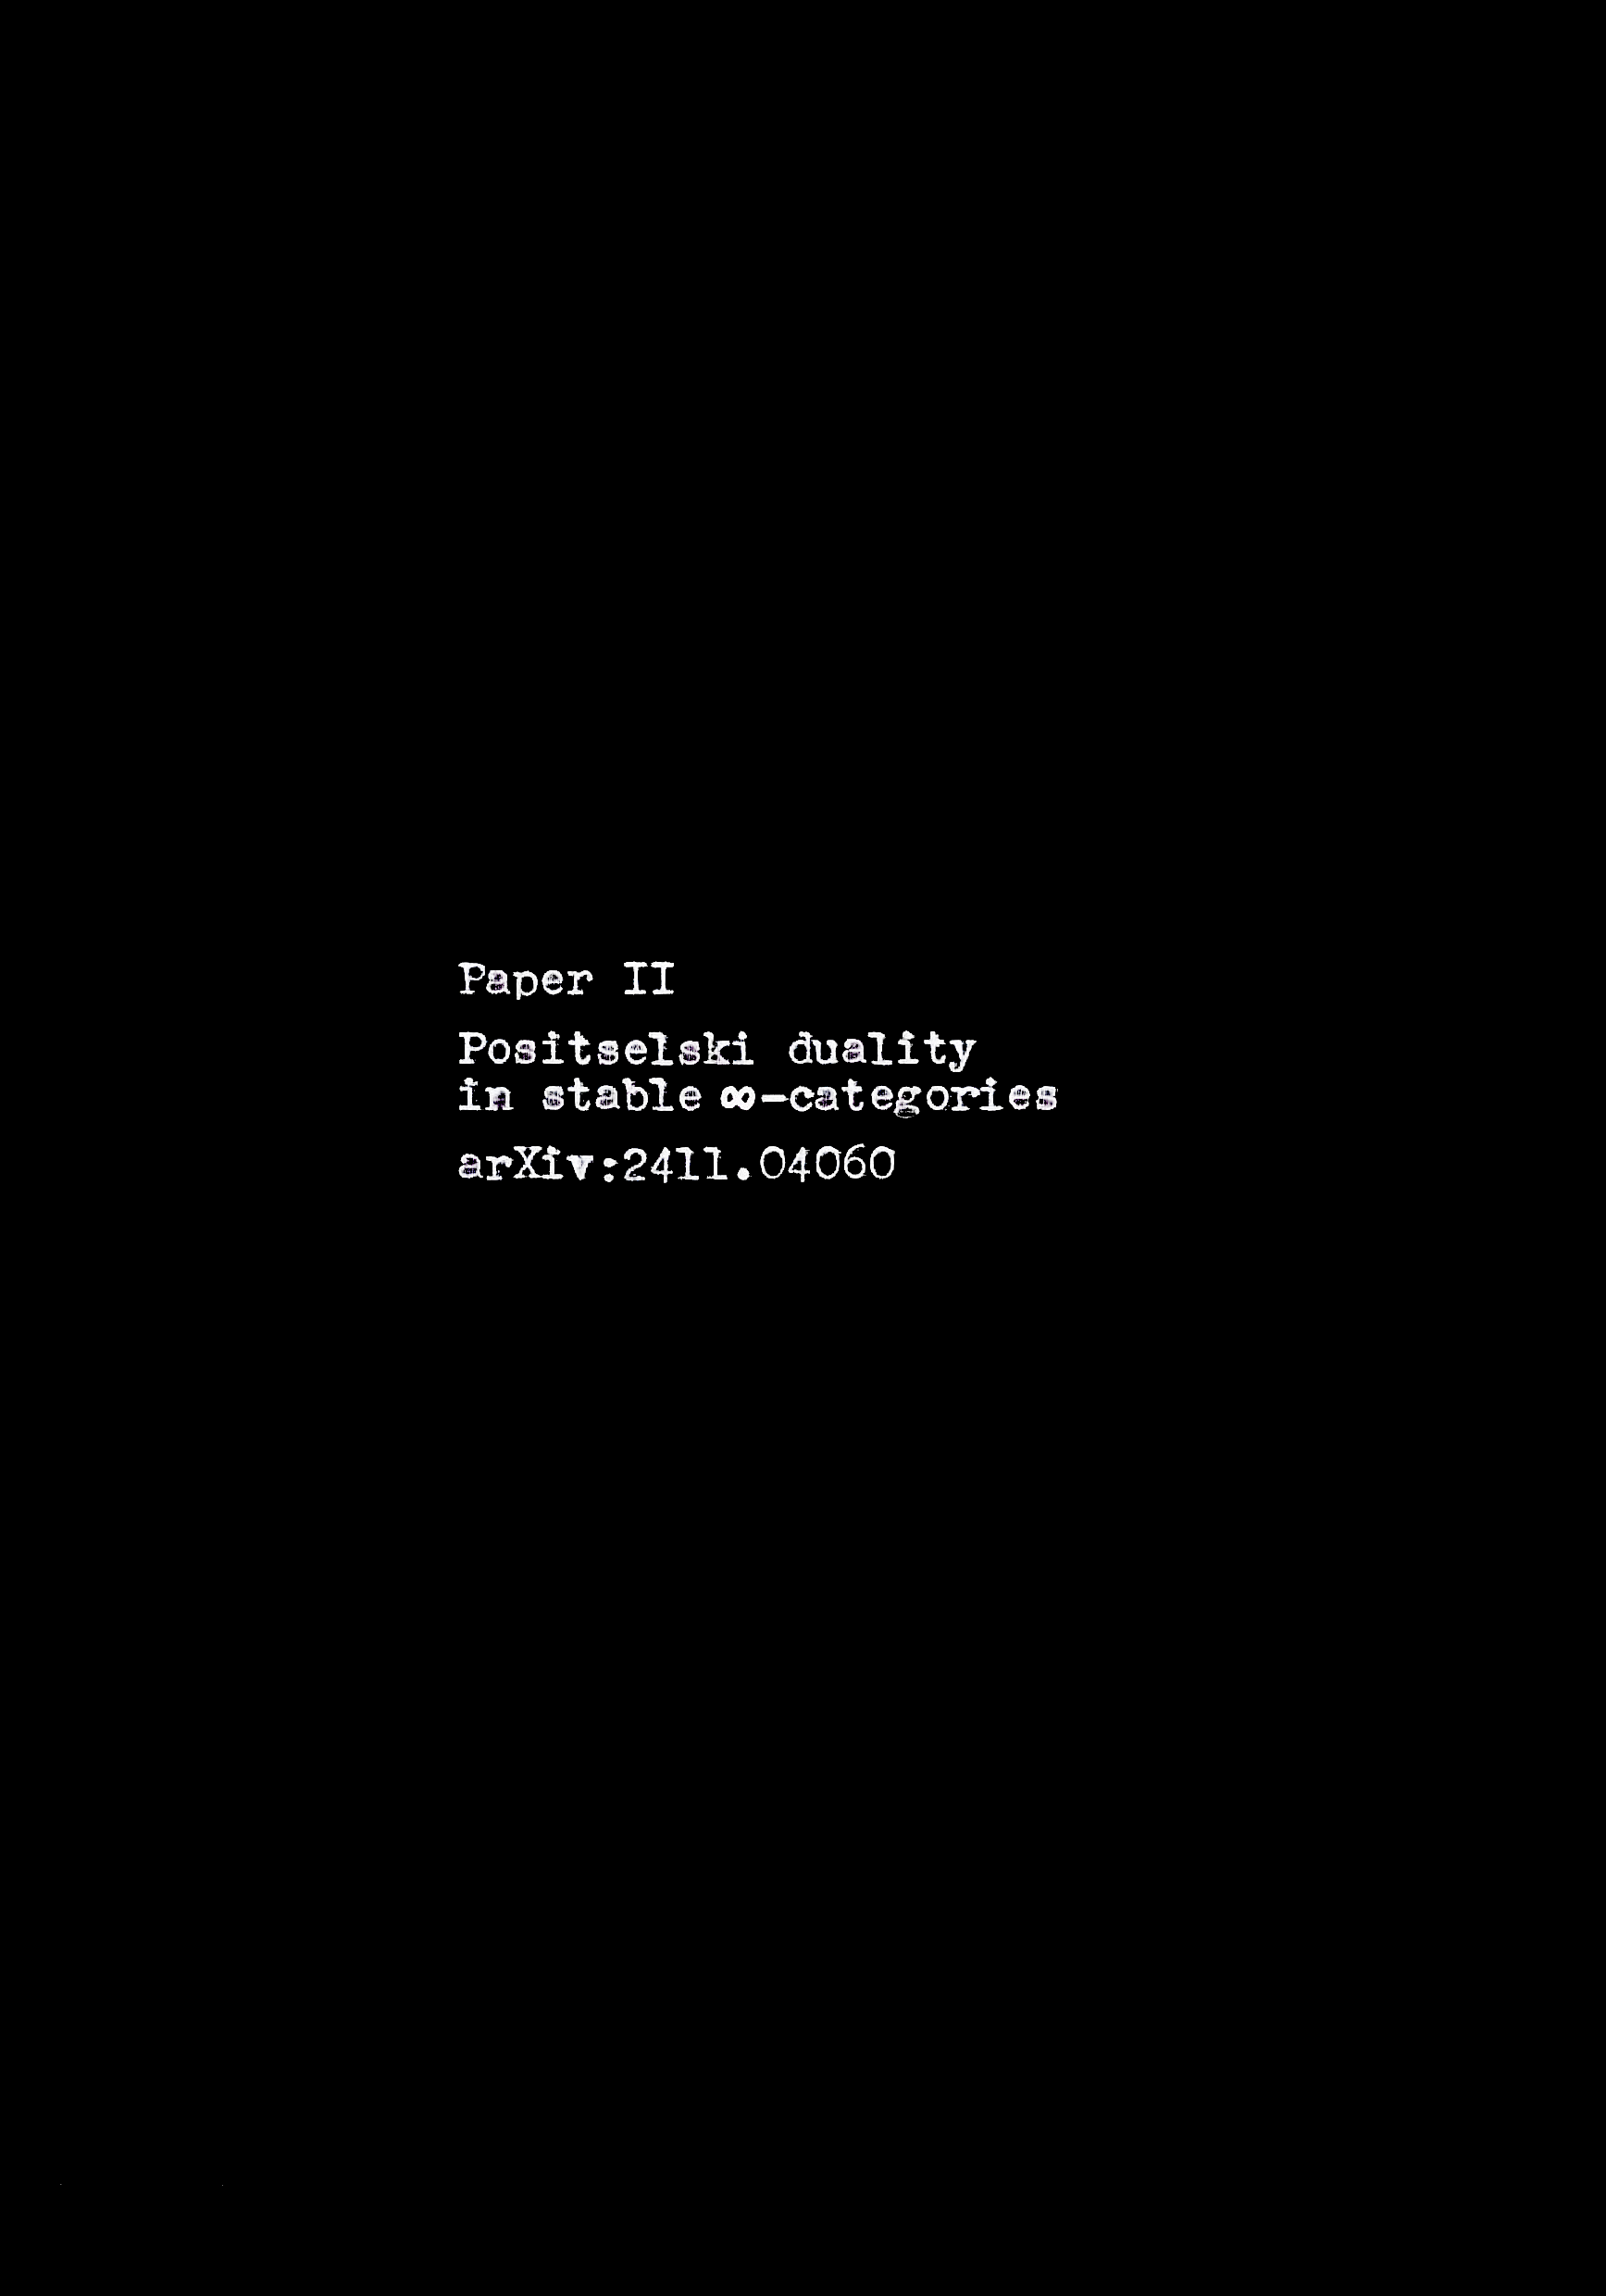
\includegraphics[%
clip,
width=1.05\paperwidth,
height=1.05\paperheight
]{chaptertitles/paper2b.png}};

\clearpage


\newpage
\tikz[remember picture,overlay]\node[opacity=1,inner sep=0pt] at (current page.center)%
{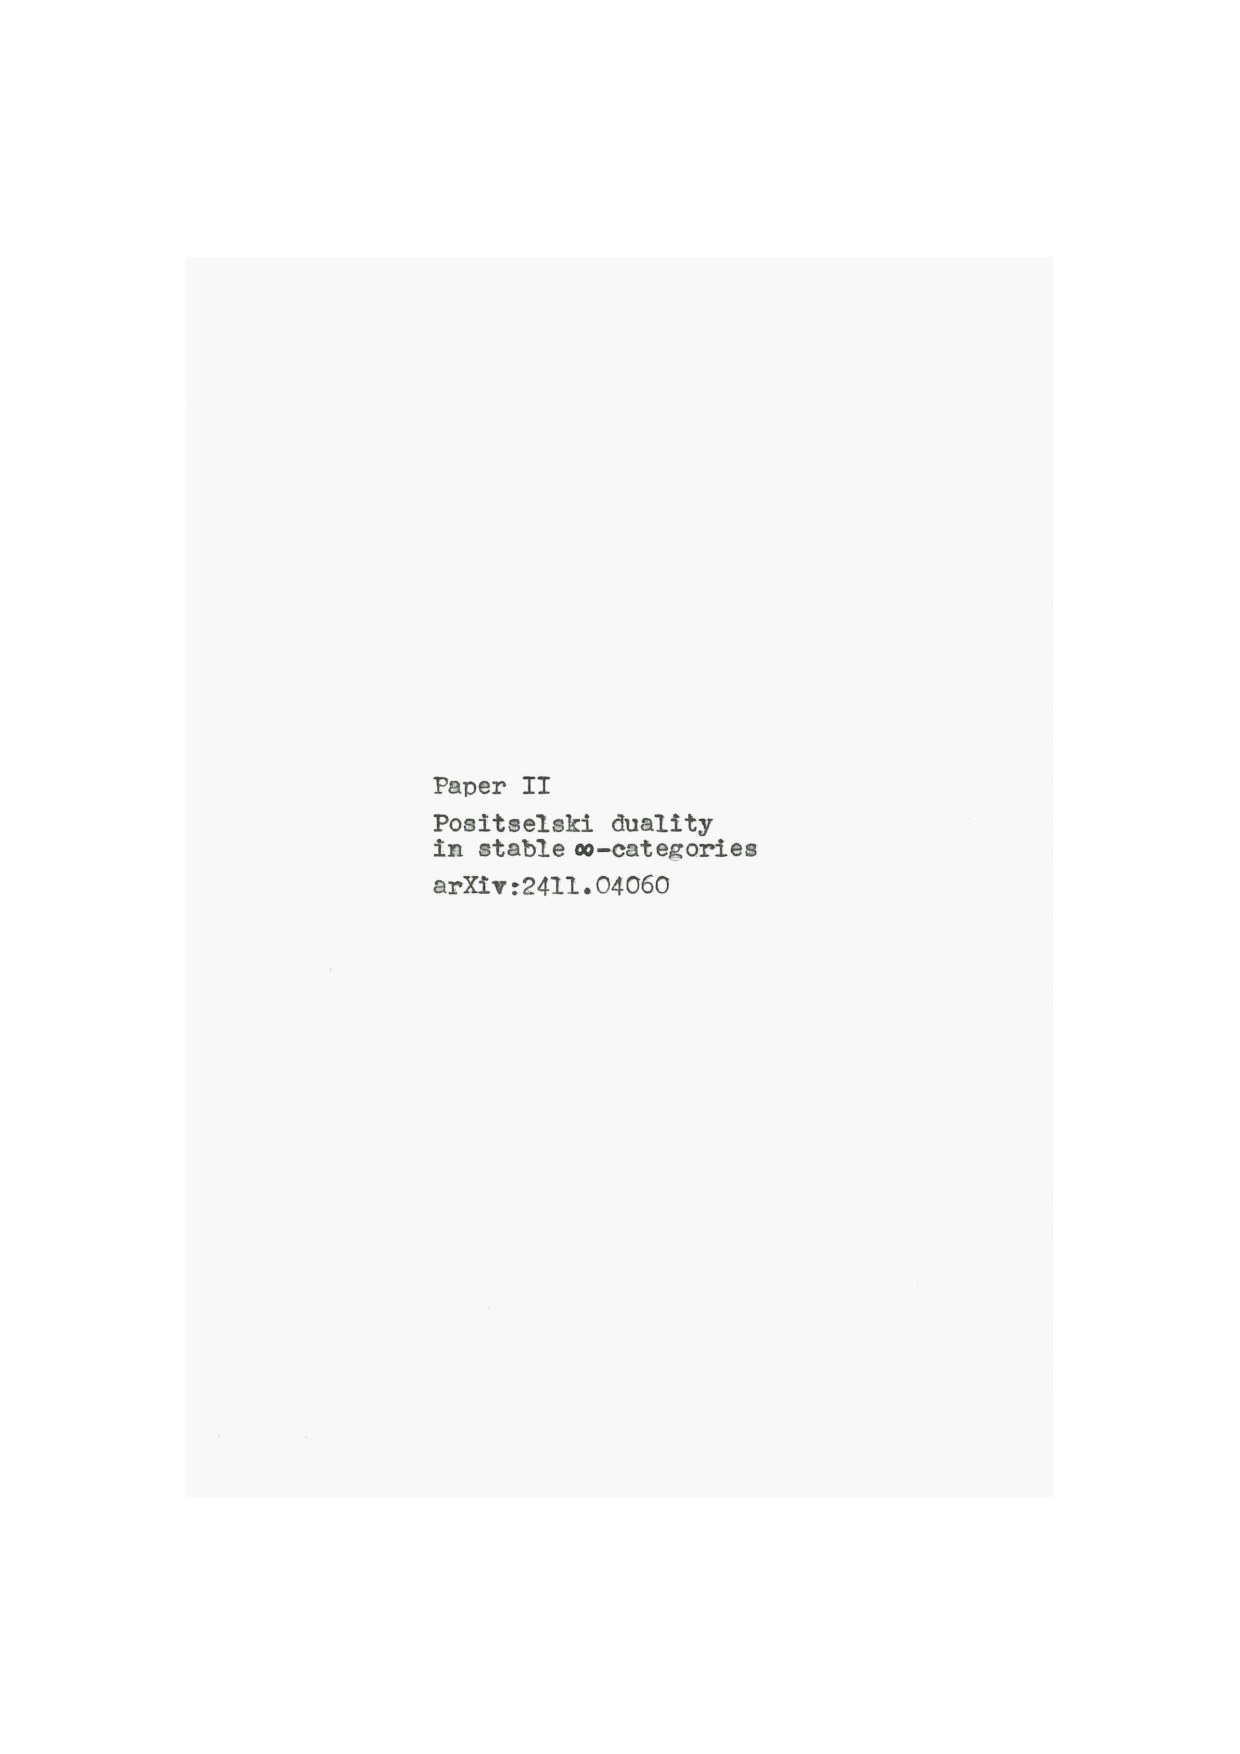
\includegraphics[%
clip,
width=1.05\paperwidth,
height=1.05\paperheight
]{chaptertitles/paper2.pdf}};

\clearpage


\subsection*{Description}

The main result of the second paper concerns a mathematical concept called a duality theory. A duality is a way to view a collection of objects ``through a mirror'' and study their reflections instead of their direct features. Studying a concept in its mirror image, and then dualizing, should be equivalent to studying the concept directly. This mathematical mirror can be a wide variety of things, but for the drawing we have chosen a classical planar mirroring to signify this effect. The flowing lines of each of the boxes are precisely mirror images of each other, along the symmetry line right in the middle. 

The colors again have no mathematical meaning; they are there only to add visual interst, and to connect to the colors of the papers. 

\newpage

\vspace*{7cm}
\begin{verse}
    \hspace{8em}Choose a context and take your seat. \\
    \vspace{5pt}
    \hspace{8em}I have prepared the following treat. \\
    \vspace{5pt}
    \hspace{8em}The hom-tensor adjunction, \\
    \vspace{5pt}
    \hspace{8em}makes the following function: \\
    \vspace{5pt}
    \hspace{8em}Being contra is equivalent to complete. 

    %\hspace{\fill}-- Torgeir Aambø
\end{verse}\newpage


\vspace*{5cm}

{\par\centering {\Large \textbf{Abstract:}}\par}
\vspace{-2em}
\rule[-11pt]{\textwidth}{1pt}
\rule{\textwidth}{0.5pt}
    
We introduce the notion of a contramodule over a cocommutative coalgebra in a presentably symmetric monoidal $\infty$-category $\C$. Based on this we prove that local duality, in the sense of Hovey--Palmieri--Strickland and Dwyer--Greenlees, is equivalent to Positselski's comodule-contramodule correspondence for coidempotent cocommutative coalgebras in compactly generated symmetric monoidal stable $\infty$-cateogories. This gives new descriptions of the categories of $K_p(n)$-local and $T_p(n)$-local spectra. 

\rule{\textwidth}{0.5pt}
\rule[11pt]{\textwidth}{1pt}
\vspace{\fill}



\section{Introduction}

Let $k$ be a field and a $C$ a cocommutative coalgebra in the abelian category $\Vect_k$. A \emph{comodule} over $C$ is a vector space $V$ together with a coassociative counital map $V\to V\otimes_k C$. These objects were introduced in the seminal paper \cite{eilenberg-moore_65} and are categorically dual to modules over algebras. In the same paper Eilenberg and Moore introduced a further dual to comodules, which they called \emph{contramodules}. These are vector spaces $V$ with a map $\Hom_k(C, V)\to V$ satisfying similar axioms called contra-associativity and contra-unitality. 

While modules and comodules got their fair share of fame throughout the decades following their introduction, contramodules were seemingly lost to history---virtually forgotten---until dug out from their grave of obscurity by Positselski in the early 2000's. Positselski has since developed a considerable body of literature on contramodules, see for example \cite{positselski_2010, positselski_2011, positselski_2016, positselski_2017_contraadjusted, positselski_2020} or the survey paper \cite{positselski_2022_contramodules}. 

In \cite{positselski_2010} Positselski introduced the co/contra correspondence, which is an adjunction between the category of comodules and the category of contramodules over a cocommutative coalgebra $C$. This correspondence sat existing duality theories on a common footing, for example Serre--Grothendieck duality and Feigin--Fuchs central charge duality. Positselski also introduced the coderived and contraderived categories of $C$-comodules and $C$-contramodules respectively, and used this to prove a derived co/contra correspondence of the form 
\[\Der^{co}(\ComodC)\simeq \Der^{contra}(\ContraC),\]
generalizing Matlis--Greenlees--May duality and Dwyer--Greenlees duality---see \cite{positselski_2016}. 

The goal of the present paper is to extend the co/contra correspondence---which we will refer to as Positselski duality---to cocommutative coalgebras in $\infty$-categories. We will also use the correspondence in stable $\infty$-categories, which are natural enhancements of triangulated categories. These serve as the natural place to study similar correspondences and equivalences as in the derived co/contra correspondence. The canonical references for $\infty$-categories are \cite{lurie_09} and \cite{Lurie_HA}, which we will freely use throughout the paper. 




\subsection*{Motivation}

Let us try to both make a motivation for the traditional Positselski duality theory and for the connection to coalgebras in stable $\infty$-categories. 

We let $X$ be a separated noetherian scheme, $U\subset X$ an open subscheme and denote by $Z = X\backslash U$ its closed complement. The derived category of all $\O_X$-modules, $\Der(\O_X)$, has a full subcategory $\Der(X)$ consisting of complexes with quasi-coherent homology. We define $\Der(U)$ similarly. These are all stable $\infty$-categories. The homotopy category $h\Der(X)$ is precisely the more traditional triangulated derived category of $X$. 

Letting $i\:U\to X$ denote the inclusion we get an induced functor 
\[i^*\: \Der(X)\to \Der(U)\]
by pulling back along $i$. This has a fully faithful right adjoint $i_*\: \Der(U)\to \Der(X)$, which itself has a further right adjoint $i^!\: \Der(X)\to \Der(U)$. The kernels of $i^*$ and $i^!$ determine two equivalent subcategories of $\Der(X)$, the former of which is the full subcategory $\Der_Z(X)\subseteq \Der(X)$ consisting of complexes with homology supported on $Z$. Denoting by $j\: Z\to X$ the other inclusion we obtain symmetric monoidal stable recollement
\begin{center}
    \begin{tikzcd}
        \Der_Z(X) 
        \arrow[rd, yshift=2pt, xshift=1pt, "j_!"] 
        \arrow[dd, "\simeq"] 
        && \\
        
        &\Der(X) 
        \arrow[lu, yshift=-2pt, xshift=-1pt, "j^!"] 
        \arrow[ld, yshift=2pt, xshift=-1pt, "j^*", swap] 
        \arrow[r, yshift=5pt, bend left, "i^*"] 
        \arrow[r, yshift=-5pt, bend right, "i^!"] 
        &\Der(U) \arrow[l, "i_*", swap] \\
        
        \Der(X)^\wedge_Z \arrow[ru, yshift=-2pt, xshift=1pt, "j_*", swap]  
        &&                  
    \end{tikzcd}
\end{center}
where $\Der(X)^\wedge_Z$ denotes the quasi-coherent sheaves on a formal open neighborhood of $Z$. As mentioned, the categories on the left are equivalent, and are the kernels of $i^*$ and $i^!$. 

This equivalence does not on the surface have anything to do with comodules or contramodules, so let us fix this. For simplicity we assume that $X = \Spec(\Z)$, such that $\Der(X)\simeq \Der(\Z)$. Any prime $p$ determines a closed subscheme $P$ of $X$. With this setup we can identify $\Der_P(X) \simeq \Der(\Comod_{\Z/p^\infty})$ and $\Der(X)^\wedge_Z\simeq \Der(\Contra_{\Z/p^\infty})$, where $\Z/p^\infty$ is the $p$-Prüfer coalgebra of $\Z$. It is the Pontryagin dual of the $p$-adic completion of $\Z$, often denoted $\Z_p$. 

\begin{introrm}
    There is a more familiar description of $\Comod_{\Z/p^\infty}$ as the $p$-power torsion objects in $\Mod_\Z$ and $\Contra_{\Z/p^\infty}$ as the $L$-complete objects in $\Mod_\Z$. The above then reduces to the derived version of Grothendieck local duality by Dwyer--Greenlees, showing that this is a certain version of Positselski duality. In \cite[2.2(1), 2.2(3)]{positselski_2017_abelian} Positselski proves that the derived complete modules also correspond to a suitably defined version of contramodules over an adic ring. For the above example this is precisely the $p$-adic integers $\Z_p$. The comodules over $\Z/p^\infty$ then correspond to discrete $\Z_p$-modules, see \cite[Sec. 1.9, Sec. 1.10]{positselski_2022_contramodules}. 
\end{introrm}


The above motivates the classical co/contra correspondence, so let us now see how we wish to abstract this.  

As $i^*$ is a symmetric monoidal localization the category $\Der_Z(X)$ is a localizing ideal. By \cite[6.8]{rouquier_2008} there is a compact object $F\in \Der(X)$ with homology supported on $Z$ such that $F$ generates $\Der_Z(X)$ under colimits. Now, as $\Der_Z(X)$ is a compactly generated localizing ideal of a compactly generated symmetric monoidal stable $\infty$-category, the right adjoint $j^!\: \Der(X)\to \Der_Z(X)$ is smashing, hence given as $j_! j^!(\1)\otimes_{\Der(X)} (-)$, where $\1$ denotes the unit in $\Der(X)$. In $\Der(X)$ the object $j_! j^! (\1)$ is the fiber of the unit map $\1\to i_* i^* (\1)$. In fact, $i_* i^* (\1)$ is an idempotent commutative algebra in $\Der(X)$, hence the fiber of the unit map, i.e. $j_! j^!(\1)$, is a coidempotent cocommutative coalgebra. 

Using a dual version of Barr--Beck monadicity, see \cref{ch2:ssec:dual-barr-beck}, one can prove that 
\[\Der_Z(X)\simeq \Comod_{j_! j^! (\1)}(\Der(X)).\] 
Similarly, there is an equivalence 
\[\Der(X)^\wedge_Z \simeq \Contra_{j_! j^! (\1)}(\Der(X)),\]
which, put together gives us an instance of Positselski duality for stable $\infty$-categories:
\[\Comod_{j_! j^! (\1)}(\Der(X)) \simeq \Contra_{j_! j^! (\1)}(\Der(X)).\]
This is a special case of our second main theorem, \cref{ch2:introthm:B}, which is an application of the Positselski duality for commutative coalgebras  set up in \cref{ch2:introthm:A}. 
 

\subsection*{Overview of results}

As mentioned, the main goal of this paper is to introduce the notion of comodules and contramodules in $\infty$-categories. Our main result is the following. 

\begin{introthm}[{\cref{ch2:thm:Positselski-duality-coidempotent}}]
    \label{ch2:introthm:A}
    Let $\C$ be a presentably symmetric monoidal $\infty$-category. For any coidempotent cocommutative coalgebra $C$, there are mutually inverse symmetric monoidal equivalences
    \begin{center}
        \begin{tikzcd}
            \Comod_C(\C) \arrow[r, yshift=2pt, "\simeq"] & \Contra_C(\C) \arrow[l, yshift=-2pt]
        \end{tikzcd}
    \end{center}
    given by the free contramodule and cofree comodule functor respectively. 
\end{introthm}

Our main application of this is to give an alternative perspective on local duality, in the sense of \cite{hovey-palmiery-strickland_97} and \cite{barthel-heard-valenzuela_2018}. 

\begin{introthm}[{\cref{ch2:thm:local-duality-co-contra}}]
    \label{ch2:introthm:B}
    Let $(\C, \K)$ be a pair consisting of a rigidly compactly generated symmetric monoidal stable $\infty$-category $(\C, \otimes, \1)$ and $\K\subseteq \C$ a set of compact objects. If $\Gamma$ denotes the right adjoint to the fully faithful inclusion of the localizing tensor ideal generated by $\K$, i.e. $i\:\C\Ktors:= \Loc_\C^\otimes (\K)\hookrightarrow \C$, then Positselski duality for the cocommutative coalgebra $i\Gamma \1$, recovers the local duality equivalence $\C\Ktors \simeq \C\Kcomp$. 
\end{introthm}

As an example of why the two theorems above might be interesting, we have the following descriptions of the categories $\Sp_\Kpn$ and $\Sp_{T_p(n)}$ in chromatic homotopy theory. 

\begin{introcor}
    If $p$ is a prime, $n$ a non-negative integer, $\Kpn$ the associated Morava $K$-theory and $T_p(n)$ an associated telescope spectrum, then there are equivalences 
    \[\SpKpn\simeq \Contra_{M\np\S}(\Sp\np) \text{ and } \Sp_{T_p(n)}\simeq \Contra_{M\np^f \S}(\Sp\np^f)\]
    of symmetric monoidal stable $\infty$-categories. 
\end{introcor}



% \subsection*{Conventions}

% We freely use the notion of $\infty$-categories, as developed by Lurie in \cite{lurie_09} and \cite{Lurie_HA}. Unless otherwise stated, all coalgebras (resp. algebras) will be fully coherently cocommutative (resp. commutative).


\subsection*{Acknowledgements and personal remarks}

The contents of this paper go back to one of the first ideas I had at the beginning of my PhD. I had my two favorite mathematical hammers---local duality and the monoidal Barr--Beck theorem---and was trying to see if these were really one and the same tool. Local duality consists of three parts: local objects, torsion objects and complete objects. The core idea came from the fact that the local objects are modules over an idempotent algebra, and I thus wanted a similar description of the other two parts. Drew Heard's guidance led me to a dual monoidal Barr--Beck result, checking off the torsion part. I got the first hints of the last piece after an email correspondence with Marius Nielsen, where we discussed a local duality type statement for mapping spectra. The solution clicked into place during a research visit to Aarhus University. During my stay Sergey Arkhipov gave two talks on contramodules, for completely unrelated reasons, and I immediately knew this was the last piece of the puzzle. Greg Stevenson taught me some additional details, solidifying my ideas, which led me to conjecture one of the main results of the present paper during my talk in their seminar. The crowd nodded in approval, thus, being satisfied I knew the answer, I naturally spent almost two years not writing it up. 

I want to thank all of the people mentioned above for their insights and pathfinding skills, without which this project would still have been a rather simple-minded idea in the optimistic brain of a young PhD student. 


\section{General preliminaries}

The goal of this section is to introduce comodules and contramodules over an cocommutative coalgebra in some $\infty$-category $\C$. In order to do this we first review some basic facts about coalgebras, monads and comonads. 

We will for the rest of this section work in some fixed presentably symmetric monoidal $\infty$-category $\C$. In other words, $\C$ is a commutative algebra object in $\PrL$, the category of presentable $\infty$-categories and left adjoint functors. In particular, the monoidal product, which we denote by $-\otimes-\:\C\times \C\to\C$ preserves colimits in both variables. We denote the unit of the monoidal structure by $\1$. \index{Presentable $\infty$-category!Symmetric monoidal}


\subsection{Coalgebras, monads and comonads}

We denote the category of commutative algebras in $\C$ by $\CAlg(\C)$\index{Cocommutative coalgebra}. These are the coherently commutative ring objects in $\C$. By \cite[2.4.2.7]{Lurie_HA} there is a symmetric monoidal structure on $\C\op$, and we define the category of cocommutative coalgebras in $\C$ to be the category $\cCAlg(\C):= \CAlg(\C\op)\op$. Classical coalgebras will be referred to as \emph{discrete}\index{Cocommutative coalgebra!Discrete} in order to avoid confusion. 

\begin{proposition}
    The following properties hold for the category $\cCAlg(\C)$. 
    \begin{enumerate}
        \item The forgetful functor $U\:\cCAlg(\C)\to \C$ is conservative and creates colimits. \label{ch2:prop:properties-coalgebras:item1}
        \item The categorical product of two coalgebras $C, D$ is given by the tensor product of their underlying objects $C\otimes D$. \label{ch2:prop:properties-coalgebras:item2}
        \item The category $\cCAlg(\C)$ is presentably symmetric monoidal when equipped with the cartesian monoidal structure. In particular, this means that the forgetful functor $U$ is symmetric monoidal. \label{ch2:prop:properties-coalgebras:item3}
        \item The forgetful functor $U$ has a lax-monoidal right adjoint $cf\:\C\to\cCAlg(\C)$. The image of an object $X\in \C$ is called the cofree coalgebra on $X$. \label{ch2:prop:properties-coalgebras:item4}
    \end{enumerate}
\end{proposition}
\begin{proof}
    The presentability and creation of colimits by the forgetful functor is proven in \cite[3.1.2]{lurie_2018_ELL1} and \cite[3.1.4]{lurie_2018_ELL1}. The cartesian symmetric monoidal structure on $\cCAlg(\C)$ follows from \cite[3.2.4.7]{Lurie_HA}. The last item follows from the first three together with the adjoint functor theorem, \cite[5.5.2.9]{lurie_09}. 
\end{proof}

% Old proof 
% \cref{ch2:prop:properties-coalgebras:item1} follows from \cite[3.2.2.5, 3.2.2.6]{Lurie_HA} while \cref{ch2:prop:properties-coalgebras:item2} follows from \cite[3.2.4.7]{Lurie_HA}. \cref{ch2:prop:properties-coalgebras:item3} is \cite[3.1.4]{lurie_2018_ELL1}, while \cref{ch2:prop:properties-coalgebras:item4} follows from \cref{ch2:prop:properties-coalgebras:item1} and \cref{ch2:prop:properties-coalgebras:item3} via the adjoint functor theorem \cite[5.5.2.9]{lurie_09}. 


Given any $\infty$-category $\D$, the category of endofunctors $\Fun(\D, \D)$ can be given the structure of a monoidal category via composition of functors. 

\begin{definition}
    \index{Monad}
    \index{Comonad}
    A monad $M$ on $\D$ is an associative algebra in $\Fun(\D, \D)$, and a comonad $C$ is a coassociative coalgebra in $\Fun(\D, \D)$. 
\end{definition}

\begin{example}
    Any adjunction of $\infty$-categories $F:\D\rightleftarrows \mathcal{E}:G$ gives rise to a monad $GF\: \D\to \D$ and a comonad $FG\:\mathcal{E}\to \mathcal{E}$. We call these the \emph{adjunction monad} and \emph{adjunction comonad} of the adjunction $F\dashv G$. 
\end{example}

The category $\D$ is left tensored over $\Fun(\D, \D)$ via evaluation of functors. Hence, for any monad $M$ on $\D$ we get a category of left modules over $M$ in $\D$. 

\begin{definition}
    \index{Monad!Eilenberg--Moore category}
    \index{Monad!Module}
    Let $\D$ be an $\infty$-category and $M$ a monad on $\D$. We define the \emph{Eilenberg--Moore category} of $M$ to be the category of left modules $\LMod_M(\D)$. Objects in $\LMod_M(\D)$ are referred to as \emph{modules over M}. 
\end{definition}

\begin{remark}
    \index{Comonad!Eilenberg--Moore category}
    \index{Comonad!Comodule}
    Dually, any comonad $C$ on $\D$ gives rise to a category of left comodules over $C$ in $\D$. We also call this the Eilenberg--Moore category of $C$, and denote it by $\LComod_C(\D)$. Its objects are referred to as \emph{comodules} over $C$. 
\end{remark}

Given a monad $M$ on $\D$ we have a forgetful functor 
\[U_M\: \LMod_M(\D)\to \D.\] 
By \cite[4.2.4.8]{Lurie_HA} this functor admits a left adjoint $F_M\: \D\to \LMod_M(\D)$ given by $X\longmapsto MX$. We call this the \emph{free module} functor. The adjunction $F_M\dashv U_M$ is called the \emph{free-forgetful} adjunction of $M$. 

\begin{definition}
    \index{Monad!-ic adjunction}
    \index{Monad!-ic functor}
    An adjunction is said to be \emph{monadic} if it is equivalent to the free-forgetful adjunction $F_M\dashv U_M$ of a monad $M$. A functor $G\: \mathcal{E}\to \D$ is called \emph{monadic} if it is equivalent to the right adjoint $U_M$ for some monadic adjunction. 
\end{definition}

The existence of the free-forgetful adjunction for a monad $M$ implies that any monad is the adjunction monad of some adjunction. However, there can be more than one adjunction $F\dashv G$ such that $M$ is the adjunction monad for this adjunction.

\begin{definition}
    \index{Monad!Free module}
    \index{Monad!Kleisli category}
    Let $\D$ be an $\infty$-category and $M$ a monad on $\D$. A left $M$-module $B\in \LMod_M(\D)$ is \emph{free} if it is equivalent to an object in the image of $F_M$. The full subcategory of free modules is called the \emph{Kleisli category} of $M$, and is denoted $\LMod_M\fr(\D)$. 
\end{definition}

The free-forgetful adjunction restricts to an adjunction on the Kleisli Category: $F_M:\D\rightleftarrows \LMod_M\fr(\D):U_M\fr$. By \cite[1.8]{christ_2023} this is the minimal adjunction with adjunction monad equivalent to $M$. Using Lurie's $\infty$-categorical version of the Barr--Beck theorem we can also identify the free-forgetful adjunction as the maximal adjunction with adjunction monad $M$. 

\begin{theorem}[{\cite[4.7.3.5]{Lurie_HA}}]
    \label{ch2:thm:Lurie-BB}
    \index{Barr--Beck}
    A functor $G\: \mathcal{E}\to \D$ of $\infty$-categories is monadic if and only if 
    \begin{enumerate}
        \item $G$ admits a left adjoint,
        \item $G$ is conservative, and
        \item the category $\mathcal{E}$ admits colimits of $G$-split simplicial objects, and these are preserved under $G$. 
    \end{enumerate}
\end{theorem}

\begin{remark}
    By definition, if a functor $G\: \mathcal{E}\to \D$ is monadic, then there is an equivalence of categories $\mathcal{E}\simeq \LMod_{GF}(\D)$, where $F$ is the left adjoint of $G$. 
\end{remark}

\begin{definition}
    \index{Comonad!Cofree comodule}
    \index{Comonad!-ic adjunction}
    Dually, given any comonad $C$ on an $\infty$-category $\mathcal{E}$, there is a forgetful functor $U_C\: \LComod_C(\mathcal{E})\to \mathcal{E}$, which admits a right adjoint 
    \[F_C\: \mathcal{E}\to \LComod_C(\mathcal{E}).\] 
    We call this the \emph{cofree comodule functor}, and hence the adjunction $U_C\dashv F_C$ is called the \emph{cofree-forgetful} adjunction of $C$. Any adjunction $F: \D \rightleftarrows \mathcal{E}:G$ equivalent to a cofree-forgetful adjunction for some comonad $C$ on $\mathcal{E}$ is said to be \emph{comonadic}. A functor $F\: \D\to \mathcal{E}$ is said to be \emph{comonadic} if it is equivalent to the left adjoint of a comonadic adjunction. 
\end{definition}

\begin{remark}
    \index{Comonad!Kleisli category}
    The essential image of $F_C$ in $\LComod_C(\mathcal{E})$ determines the Kleisli category $\LComod_C\fr(\mathcal{E})$ of cofree coalgebras. The cofree-forgetful adjunction restricts to an adjunction on cofree comodules, $U_C\fr : \LComod_C\fr(\mathcal{E})\rightleftarrows \mathcal{E}: F_C$, which is the minimal adjunction whose adjunction comonad is $C$. 
\end{remark}


\subsection{Comodules and contramodules}

Recall that we have fixed a presentably symmetric monoidal $\infty$-category $\C$. Let us now construct the monads and comonads of interest for this paper. We want to mention that the paper \cite{hristova-jones-rumynin_2023} has been of influence for this section.

\begin{example}
    \label{ch2:ex:algebra-module-monad}
    Let $A\in \CAlg(\C)$ be a commutative algebra object in $\C$. The algebra structure on $A$ induces an algebra structure on the endofunctor $A\otimes(-)\:\C\to \C$, hence it is a monad on $\C$. By \cite[1.17]{christ_2023} the Eilenberg--Moore category of this monad is equivalent to the category of modules over $A$ in $\C$. As $A$ is commutative we denote this by $\Mod_A(\C)$. As $\C$ is presentable and the monad $A\otimes(-)$ preserves colimits, there is a right adjoint $\iHom(A,-)\:\C\to \C$. This is a comonad on $\C$. Since these form an adjoint monad-comonad pair, their Eilenberg--Moore categories are equivalent,
    \[\Mod_A(\C)\simeq \LMod_{A\otimes(-)}(\C)\simeq \LComod_{\iHom(A,-)}(\C),\]
    see \cite[V.8.2]{maclane-moerdijk_1994} in the $1$-categorical situation. The $\infty$-categorical version is exactly the same, and follows from the monadicity and comonadicity of the adjunctions. 
\end{example}

\begin{remark}
    \label{ch2:rm:internal-adjunction}
    \index{Internal adjunction}
    We also mention that the hom-tensor adjunction is an \emph{internal adjunction}, in the sense that there is an equivalence of internal hom-objects 
    \[\iHom(X\otimes Y, Z) \simeq \iHom(X, \iHom(Y, Z)).\]
    This follows from the hom-tensor adjunction together with a Yoneda argument. 
\end{remark}

% Since $\C$ is a symmetric monoidal category, we can restrict our attention to \emph{monoidal monads} and \emph{monoidal comonads}. For us these are exactly the monads (resp. comonads) that appear as the adjunction monad for a monoidal adjunctions, i.e., $F:\C\rightleftarrows \D:G$ such that $F$ (resp. $G$) is symmetric monoidal. Given a monoidal monad $M$, the corresponding Eilenberg--Moore category $\LMod_M(\C)$ inherits the structure of a presentably symmetric monoidal $\infty$-category. Since $\C$ is symmetric monoidal, the tensor product of two free $M$-modules is still free, hence this restricts to a symmetric monoidal structure on $\LMod_M\fr(\C)$. 

The above example changes in an interesting way when replacing the algebra $A$ with a coalgebra $C$. 

\begin{example}
    \label{ch2:ex:coalgebra-comonad}
    Let $C\in \cCAlg(\C)$ be a cocommutative coalgebra object in $\C$. The coalgebra structure on $C$ induces a coalgebra structure on the endofunctor $C\otimes(-)\:\C\to\C$, hence it is a comonad on $\C$. By an argument dual to \cite[1.17]{christ_2023} the Eilenberg--Moore category of this comonad is equivalent to the category of comodules over the coalgebra $C$, which we denote by $\Comod_C(\C)$. The category $\Comod_C(\C)$ is presentable by \cite[3.8]{ramzi_2024}, as $C\otimes (-)$ is accessible. 
\end{example}

\begin{example}
    Let $C\in \cCAlg(\C)$ be a cocommutative coalgebra in $\C$. The comonad $C\otimes (-)$ preserves colimits, hence it has a right adjoint $\iHom(C,-)$. The coalgebra structure on $C$, together with the internal adjunction equivalence from \cref{ch2:rm:internal-adjunction}, gives the endofunctor $\iHom(C,-)$ an algebra structure. It is an algebra structure and not a coalgebra structure, as the internal hom is contravariant in the first variable. Hence, $\iHom(C,-)$ is a monad on $\C$.
\end{example} 

Notice that the pair $C\otimes(-)\dashv \iHom(C,-)$ is not an adjoint monad-comonad pair---it is now an an adjoint comonad-monad pair. The difference is subtle, but it means, in particular, that their Eilenberg--Moore categories might not be equivalent. This possible non-equivalence is the \emph{raison d'être} for contramodules, which we can then define as follows.

% \begin{lemma}
%     For any adjoint comonad-monad pair $C\dashv M$ on a presentable $\infty$-category $\C$, there is an equivalence 
%     \[\Comod\fr_C(\C)\simeq \Mod\fr_M(\C).\]
% \end{lemma}
% \begin{proof}
%     The objects in the categories are the same, given by an underlying object in $\C$ with additional structure. Hence, it is enough to show that the mapping spaces in the two categories are equivalent. Let $X, Y$ be two objects in $\C$. As the cofree comodule functor $F_C$ is right adjoint to the forgetful functor $U_C$, we get $\Hom_{\Comod_C}(F_C X, F_C Y)\simeq \Hom_\C(C (X), Y)$. By the adjunction $C\dashv M$ on $\C$ we get $\Hom_\C(C(X), Y) \simeq \Hom_\C(X, M(Y))$, which gives finally $\Hom_\C(X, M(Y))\simeq \Hom_{\Mod_M}(F_M X, F_M Y)$, as the free module functor $F_M$ is a left adjoint to the forgetful functor $U_M$.
% \end{proof}

% \begin{remark}
%     This has been noted and proved several times in the $1$-categorical literature on monads and comonads, see for example \cite[Theorem 3]{kleiner_1990}. The proof above is by \cite[2.5]{bohm-brzezinski-wisbauer_2009}. 
% \end{remark}



\begin{definition}
    \index{Contramodule}
    Let $C\in \cCAlg(\C)$ be a cocommutative coalgebra. A \emph{contramodule} over $C$ is a module over the internal hom-monad $\iHom(C,-)\:\C\to \C$. The category of contramodules over $C$ in $\C$ is the corresponding Eilenberg--Moore category, which will be denoted $\ContraC(\C)$. 
\end{definition}

\begin{notation}
    Since we are working in a fixed category $\C$ we will often simply write $\ContraC$ for the category of contramodules, and $\ComodC$ for the category of comodules. 
\end{notation}

\begin{notation}
    We denote the mapping space in $\Comod_C$ by $\Hom_C$ and the mapping space in $\Contra_C$ by $\Hom^C$. Similarly, the forgetful functors will be denoted $U_C\:\Comod_C\to \C$ and $U^C\: \Contra_C\to \C$ respectively, while their adjoints---the cofree and free functors---will be denoted $C\otimes (-)\:\C\to \Comod_C$ and $\iHom(C, -)\: \C\to \Contra_C$, hoping that it is clear from context whether we use them as above or as endofunctors on $\C$.
\end{notation}

The following proposition is standard for monads and comonads, see for example \cite[5.7]{riehl-verity_2015}. 

\begin{proposition}
    If $C$ is a cocommutative coalgebra in $\C$, then the forgetful functor $U_C\:\Comod_C\to \C$ creates colimits. Similarly, the forgetful functor $U^C\:\Contra_C\to \C$ creates limits. 
\end{proposition}







\subsection{The dual monoidal Barr--Beck theorem}
\label{ch2:ssec:dual-barr-beck}

Lurie's version of the Barr--Beck monadicity theorem, see \cite[Section 4.7]{Lurie_HA}, allows us to recognize monadic functors from simple criteria. Combined with a recognition theorem for when a monoidal monadic functor is equivalent to $R\otimes(-)$ for some commutative ring $R$, Mathew--Neumann--Noel extended the Barr--Beck theorem to a monoidal version. In this short section we prove a categorical dual version of their result. 

Let $F:\C\rightleftarrows \D:G$ be a pair of adjoint functors between presentably symmetric monoidal $\infty$-categories, such that the left adjoint $F$ is symmetric monoidal. This means that the right adjoint $G$ is lax-monoidal, and does in particular preserve algebra objects. There is for any two objects $X\in \C$ and $Y\in \D$, a natural map
\[F(G(Y)\otimes_\C X)\overset{\simeq}\to FG(Y)\otimes_\D F(X) \to Y\otimes_\D F(X)\]
where the first map is by the symmetric monoidality of $F$, and the second is given by the adjunction counit. By the adjunction property, there is an adjoint map 
\[G(Y)\otimes_\C X \to G(Y\otimes_\D F(X)).\]

\begin{definition}
    \index{Projection formula!Monadic}
    An adjoint pair $F\dashv G$ as above is said to satisfy the \emph{monadic projection formula} if the map 
    \[G(Y)\otimes_\C X \to G(Y\otimes_\D F(X))\]
    is an equivalence for all $X\in \C$ and $Y\in \D$. 
\end{definition}

We now state the monoidal Barr--Beck theorem of Mathew--Neumann--Noel. 

\begin{theorem}[{\cite[5.29]{mathew-naumann-noel_2017}}]
    \label{ch2:thm:monoidal-BB}
    \index{Barr--Beck!Monoidal}
    Let $F:\C\rightleftarrows \D:G$ be an adjunction of presentably symmetric monoidal $\infty$-categories, such that the left adjoint $F$ is symmetric monoidal. If, in addition
    \begin{enumerate}
        \item $G$ is conservative,
        \item $G$ preserves arbitrary colimits, and
        \item $F\dashv G$ satisfies the monadic projection formula,
    \end{enumerate}
    then the adjunction is monoidally monadic, and there is an equivalence of monads 
    \[GF \simeq G(\1_\D)\otimes_\C(-).\]
    In particular, there is an equivalence $\D\simeq \Mod_{G(\1_\D)}(\C)$ of symmetric monoidal $\infty$-categories. 
\end{theorem}

\begin{remark}
    Note that this result is stated only for stable $\infty$-categories in \cite{mathew-naumann-noel_2017}, but also holds unstably by a combination of Lurie's $\infty$-categorical Barr--Beck theorem, \cref{ch2:thm:Lurie-BB}, together with the fact that the monadic projection formula applied to the unit gives an equivalence of monads by \cite[3.6]{elmanto-kolderup_2020}. 
\end{remark}

There is also a dual version of the classical Barr--Beck theorem, see for example \cite[4.5]{brantner-mathew_2023}. We wish to extend this to a monoidal version. 

Let $F:\C\rightleftarrows \D:G$ pair of adjoint functors between symmetric monoidal categories, such that the right adjoint $G$ is symmetric monoidal. This means that the left adjoint $F$ is op-lax-monoidal, and does in particular preserve coalgebra objects. There is for any two objects $X\in \C$ and $Y\in \D$, a natural map
\[X\otimes_\C G(Y)\to GF(X)\otimes_\C G(Y) \overset{\simeq}\to G(F(X)\otimes_\D Y)\]
where the first map is given by the adjunction unit and the second by the symmetric monoidality of $G$. By the adjunction property, there is an adjoint map 
\[F(X\otimes_\C G(Y)) \to F(X)\otimes_\D Y .\]

\begin{definition}
    \index{Projection formula!Comonadic}
    An adjoint pair $F\dashv G$ as above is said to satisfy the \emph{comonadic projection formula} if the map 
    \[F(X\otimes_\C G(Y)) \to F(X)\otimes_\D Y\]
    is an equivalence for all $X\in \C$ and $Y\in \D$. 
\end{definition}

\begin{theorem}
    \index{Barr--Beck!Dual monoidal}
    \label{ch2:thm:dual-monoidal-BB}
    Let $F:\C\rightleftarrows \D:G$ be an adjunction of presentably symmetric monoidal $\infty$-categories, such that the right adjoint $G$ is symmetric monoidal. If, in addition
    \begin{enumerate}
        \item $F$ is conservative,
        \item $F$ preserves arbitrary limits, and
        \item $F\dashv G$ satisfies the comonadic projection formula,
    \end{enumerate}
    then the adjunction is comonadic, and there is an equivalence of comonads 
    \[FG\simeq F(\1_C)\otimes_\D (-)\] 
    In particular, this gives an equivalence $\C\simeq \Comod_{F(\1_\C)}(\D).$
\end{theorem}

\begin{remark}
    Before the proof, let us explain intuitively why the statement makes sense. The unit $\1_\C$ in a presentably symmetric monoidal $\infty$-category $\C$ is both a commutative algebra\index{Commutative algebra} and a cocommutative coalgebra\index{Cocommutative coalgebra}. In the above adjunction we have that the right adjoint $G$ is symmetric monoidal, hence its left adjoint $F$ is op-lax monoidal. In particular, it sends coalgebras to coalgebras, meaning that $F(\1_\C)$ is an cocommutative coalgebra in $\D$. By \cref{ch2:ex:coalgebra-comonad} tensoring with $F(\1_\C)$ is a comonad, not a monad, as for \cref{ch2:thm:monoidal-BB}. 
\end{remark}

\begin{proof}
    By \cite[4.5]{brantner-mathew_2023} the adjunction is comonadic. A dual version of \cite[3.6]{elmanto-kolderup_2020} shows that there is a map of comonads $\phi\: FG \to F(\1_\C)\otimes_\D (-)$, and consequently an adjunction 
    \begin{center}
        \begin{tikzcd}
            \Comod_{FG}(\D) \arrow[r, yshift=2pt, "\phi_*"] & \Comod_{F(\1_\C)\otimes_\D (-)}(\D) \arrow[l, yshift=-2pt, "\phi^*"]
        \end{tikzcd}
    \end{center}
    By applying the projection formula to the unit $\1_\C$ we get that $\phi$ is a natural equivalence, which means that the adjunction $(\phi_*, \phi^*)$ is an adjoint equivalence. By \cref{ch2:ex:coalgebra-comonad} the Eilenberg--Moore category of the comonad $F(\1_\C)\otimes_\D (-)$ is equivalent to the category of comodules over the cocommutative coalgebra $F(\1_\C)$, finishing the proof. 
\end{proof}

\begin{remark}
    \label{ch2:rm:monoidal-structure-comodules}
    We want to specify when the above equivalence is an equivalence of symmetric monoidal categories. We could hope for the existence of a symmetric monoidal structure on $\Comod_C$ for a cocommutative coalgebra $C\in \C$. For the category $\Mod_R(\C)$ of modules over a commutative algebra $R\in \C$ this is done by Lurie's relative tensor product, see \cite[Section 4.5.2]{Lurie_HA}. But, for such a relative monoidal product to exist on $\Comod_C$ one needs the tensor product in $\C$ to commute with cosifted limits, which is rarely the case. But, as we will see in \cref{ch2:ssec:coidempotent-coalgebras} we sometimes get a monoidal structure, and when this is the case, the equivalence in \cref{ch2:thm:dual-monoidal-BB} is symmetric monoidal. 
\end{remark}



\section{Positselski duality}
\label{ch2:sec:positselski-duality}

Classical Positselski duality, usually called the co-contra correspondence, is an adjunction between comodules and contramodules over a discrete $R$-coalgebra $C$, where $R$ is an algebra over a field $k$. In particular, the categories involved are abelian, which makes some constructions easier. For example, the monoidal structure on $\Mod_R$ induces monoidal structures on $\Comod_C$ via the relative tensor construction---given by a certain equalizer. For $\infty$-categories the relative tensor construction is more complicated, as we need the monoidal structure to behave well with all higher coherencies, as mentioned in \cref{ch2:rm:monoidal-structure-comodules}. We can, however, restrict our attention to a certain type of coalgebra, fixing these issues. This also puts us in the setting we are interested in regarding local duality---see \cref{ch2:ssec:local-duality}. 

\subsection{Coidempotent coalgebras}
\label{ch2:ssec:coidempotent-coalgebras}

We now restrict our attention to a special class of coalgebras, which will be our focus on for the remainder of the paper. 

\begin{definition}
    %\index{Cocommutative coalgebra!Separable}
    \index{Cocommutative coalgebra!Coidempotent}
    A cocommutative coalgebra $C\in \cCAlg(\C)$ is said to be \emph{coidempotent} if the comultiplication map 
    \[\Delta\: C\to C\otimes C\] 
    is an equivalence. 
\end{definition}

% \begin{remark}
%     \label{ch2:rm:coidempotent-implies-separable}
%     Any coidempotent coalgebra is in particular separable, see \cite[1.6(1)]{ramzi_2023} for a formally dual statement. 
% \end{remark}

The first reason for our focus on coidempotent coalgebras is that their categories of comodules inherit a symmetric monoidal structure from $\C$, which is rarely the case for general coalgebras, see \cref{ch2:rm:monoidal-structure-comodules}. 

\begin{lemma}
    \label{ch2:lm:coidempotent-then-comod-monoidal}
    \index{Colocalization!Smashing}
    Let $C$ be a coidempotent cocommutative coalgebra in $\C$. The category of $C$-comodules $\Comod_C$ inherits the structure of a presentably symmetric monoidal $\infty$-category making the cofree comodule functor a symmetric monoidal smashing colocalization. Furthermore, any $C$-comodule is cofree, meaning that the fully faithful inclusion $\Comod_C\fr \hookrightarrow \Comod_C$ is a symmetric monoidal equivalence. 
\end{lemma}
\begin{proof}
    By a dual version of \cite[4.8.2.4]{Lurie_HA}, together with \cref{ch2:ex:coalgebra-comonad}, the category $\Comod_C$ is a colocalization of $\C$. This implies, by a dual version of \cite[4.8.2.7]{Lurie_HA}, that $\Comod_C$ inherits a symmetric monoidal structure from $\C$. Finally, a dual version of \cite[4.8.2.10]{Lurie_HA} implies that the inclusion of cofree comodules to all comodules is an equivalence. 

    The category $\Comod_C$ is presentable by \cite[2.1.11]{peroux_2020}, which together with \cref{ch2:prop:creates-colimits-and-limits} implies that $\Comod_C$ is presentably symmetric monoidal. 
\end{proof}

\begin{remark}
    \label{ch2:rm:unique-structure}
    As stated in \cref{ch2:lm:coidempotent-then-comod-monoidal}, any comodule over a coidempotent coalgebra is cofree. This implies that any comodule has a unique comodule structure. In particular, the structure map $M \to C\otimes M$ for any $C$-comodule $M$ is an equivalence, meaning that the induced tensor product on $\Comod_C$ can be interpreted as simply taking the tensor product of the underlying objects in $\C$. More precisely, the monoidal structure on $\Comod_C$ is given by $M\otimes_C N := C\otimes (M\otimes N)$, but by the uniqueness of comodule structures, this is simply $M\otimes N$ when treated as an object in $\C$. 
    % The existence of a symmetric monoidal structure will follow from the fact that comodules over coidempotent coalgebras admit unique comodule structures. In particular, if $M$ is a comodule, then the structure map $M \to C\otimes M$ is an equivalence, meaning that $M$ is equivalent to the cofree comodule on its underlying object. This means that any comodule over a coidempotent coalgebra is cofree, giving an equivalence 
    % \[\Comod_C \simeq \Comod_C\fr\]
    % between the Eilenberg--Moore category and the Kleisli category of the comonad $C\otimes (-)$ on $\C$. 
\end{remark}

    % Let $M$ and $N$ be two comodules, and define the tensor product $M\otimes_C N$ to be the tensor product of their underlying objects. By the uniqueness of comodule structures, this still results in a comodule structure on the product, as $M \otimes_C N \simeq M \otimes N \otimes C$, which is the cofree comodule on the underlying object. 
    
    % This means, in particular, that the cofree comodule functor $C\otimes (-) \: \C \to \Comod_C$ is symmetric monoidal by \cite[2.2.1.9]{Lurie_HA}. As the endofunctor $C\otimes (-) \: \C \to \C$ is idempotent, and the forgetful functor $U_C\: \Comod_C\to \C$ is fully faithful whenever $C$ is coidempotent, we can conclude that the cofree comodule functor $C\otimes (-)\: \C\to \Comod_C$ is a smashing colocalization of $\C$. 

% The co-bar construction starts at n=0, hence this does not work (as commented by Irakli):

%Their relative tensor product in $\Comod_C$ is defined by the the two sided co-bar construction,
%\[M\otimes_C N := \lim_n (M \otimes C^{\otimes n} \otimes N),\]
%but, as $C$ is coidempotent this is just the object $N\otimes C\otimes M$, which is the cofree comodule on the underlying object of $M\otimes N$. This means that the relative tensor product is defined for all comodules. The unit for the monoidal structure $-\otimes_C-$ is $C$, and the monoidal structure is symmetric monoidal as the monoidal structure in $\C$ is. 

\begin{lemma}
    The symmetric monoidal structure on the category $\Comod_C$ is closed. 
\end{lemma}
\begin{proof}
    As the cofree-forgetful adjunction creates colimits in the category $\Comod_C$, the functor 
    \[-\otimes_C- \: \Comod_C \times \Comod_C \to \Comod_C\] 
    preserves colimits separately in each variable. In particular, the functor $M\otimes_C (-)$ preserves colimits, hence has a right adjoint $\iHom_C(M,-)$ for any comodule $M$ by the adjoint functor theorem, \cite[5.5.2.9]{lurie_09}. This determines a functor 
    \[\iHom_C(-,-)\: \Comod_C\op\times \Comod_C\to \Comod_C\]
    making $\Comod_C$ a closed symmetric monoidal category.  
\end{proof}

\begin{remark}
    This adjunction, being a hom-tensor adjunction, is also internally adjoint in the sense of \cref{ch2:rm:internal-adjunction}\index{Internal adjunction}. Hence we have an equivalence 
    \[\iHom_C(M\otimes_C N, A) \simeq \iHom_C(M, \iHom_C(N, A))\]
    for all comodules $M, N$ and $A$. 
\end{remark}

%Another important reason for using coidempotent coalgebras in this paper is the following result. Recall that a comodule over a coalgebra $C$ is called cofree, if it is of the form $M\otimes C$ for some $M\in \C$. These are precisely the comodules in the image of the right adjoint to the forgetful functor $U_C\:\Comod_C\to \C$, when $C$ is coidempotent. This is a slightly weaker coalgebraic version of \cite[1.13, 1.14]{ramzi_2023}. See also \cite[3.6]{brzezinski_2010} for a related $1$-categorical version. 

% \begin{lemma}
%     \label{ch2:lm:comod-over-separable-are-cofree}
%     \index{Comonad!Cofree comodule}
%     Every comodule over a coidempotent coalgebra $C$ is a retract of a cofree comodule. In particular, there is an equivalence 
%     \[\ComodC(\C)\simeq \ComodC\fr(\C)\]
%     between the Eilenberg--Moore category and the Kleisli category of the comonad $C\otimes (-)$ on $\C$. 
% \end{lemma}
% \begin{proof}
%     As coidempotent coalgebras are separable, see \cref{ch2:rm:coidempotent-implies-separable}, the result will follow from the fact that the forgetful functor $U_C\: \Comod_C\to \C$ is separable, in the sense that the adjunction unit map 
%     \[\Id_{\Comod_C}\to C\otimes U(-)\]
%     has a $\C$-linear section, whenever $C$ is separable. The section is given by 
%     \[C\otimes M \overset{\simeq}\to (C\otimes C)\otimes_C M \to C\otimes_C M\overset{\simeq}\longleftarrow M\]
%     for any comodule $M$. 
% \end{proof}

% We get a similar statement for contramodules over $C$. Recall that a contramodule is said to be free if it is of the form $\iHom(C,M)$ for some $M\in \C$. \index{Contramodule!Free}

% \begin{proposition}
%     \label{ch2:prop:contra-over-separable-are-free}
%     Let $C\in \cCAlg(\C)$ be a separable coalgebra. Then every contramodule over $C$ is a retract of a free contramodule. In particular, there is an equivalence 
%     \[\ContraC(\C)\simeq \ContraC\fr(\C)\]
%     between the Eilenberg--Moore and Kleisli category of the monad $\iHom(C,-)$ on $\C$. 
% \end{proposition}
% \begin{proof}
%     We can prove this by showing that the section for the separable coalgebra $C$ gives a section of the forgetful functor $U^C\:\Contra_C\to \C$. The section is, for a contramodule $X$, given by the adjoint map $M\to \iHom(C, M)$ to the section of the forgetful functor $U_C$ on $\Comod_C$ from \cref{ch2:lm:comod-over-separable-are-cofree}.  
% \end{proof}


We know from \cref{ch2:lm:coidempotent-then-comod-monoidal} that the cofree comodule functor 
\[C\otimes(-)\: \C\to \Comod_C\]
is a smashing colocalization whenever the coalgebra $C$ is coidempotent. We now wish to have a similar statement for the free contramodule functor 
\[\iHom(C,-)\: \C\to \Contra_C.\]
Note that it will not be smashing in general, but otherwise it will have the same features. 

\begin{remark}
    \label{ch2:rm:contramodule-structure-on-hom-from-comodule}
    Let $M$ be a $C$-comodule and $V$ any object in $\C$. The structure map $\rho_M\: M\to C\otimes M$ induces a $C$-contramodule structure on the internal hom-object $\iHom(M, V)$, via 
    \[\iHom(C, \iHom(M, V))\simeq \iHom(C\otimes M, V)\overset{-\circ \rho_M}\to \iHom(M, V).\]
\end{remark}

\begin{lemma}
    \label{ch2:lm:free-contra-monoidal}
    \index{Presentable $\infty$-category!Symmetric monoidal}
    Let $C$ be a coidempotent cocommutative coalgebra in $\C$. The category of $C$-contramodules $\Contra_C$ inherits the structure of a presentably symmetric monoidal $\infty$-category, making the free contramodule functor a symmetric monoidal localization. In particular, all $C$-contramodules are free. 
\end{lemma}
\begin{proof}
    The functor $\iHom(C,-)\: \C \to \C$ is an idempotent functor, as we have
    \[\iHom(C, \iHom(C,-))\simeq \iHom(C\otimes C, -)\simeq \iHom(C,-)\]
    by the internal adjunction property together with the coidempotency of $C$. This means that the forgetful functor $U^C\: \Contra_C\to \C$ is fully faithful by \cite[5.2.7.4]{lurie_09}, and hence that the free contramodule functor $\iHom(C,-)\:\C\to \Contra_C$ is a localization. In particular, $\iHom(C, X) \simeq X$ for any $C$-contramodule $X$, meaning that any $C$-contramodule is free. 
    
    In order to determine that it induces a symmetric monoidal structure on $\Contra_C$ we need to check that the free functor is compatible with the monoidal structure in $\C$, in the sense of \cite[2.2.1.7]{Lurie_HA}. More precisely we need to show that if a map $V \to V'$ in $\C$ is a $\iHom(C,-)$-equivalence, then also $V\otimes W \to V' \otimes W$ is. By \cite[2.12(3)]{nikolaus_2016} this property holds whenever $\iHom(V,X)\in \Contra_C$ for any $X\in \Contra_C$ and $V\in \C$, which we now show. 
    
    As all $C$-contramodules are free, we let $X = \iHom(C, A)$ for some $A\in \C$ and $V\in \C$. By the hom-tensor adjunction we get 
    \[\iHom(V, \iHom(C, A))\simeq \iHom(C\otimes V, A).\]
    As $C\otimes V$ is a $C$-comodule, the object $\iHom(C\otimes V, A)$ is a $C$-contramodule by \cref{ch2:rm:contramodule-structure-on-hom-from-comodule}. Hence, $\iHom(C,-)$ is compatible with the monoidal structure. By \cite[2.2.1.9]{lurie_09} this implies that the free contramodule functor $\iHom(C,-)\: \C\to \Contra_C$ can be given the structure of a symmetric monoidal functor. 
    
    Finally, as $\Contra_C$ is a localization of a presentably symmetric monoidal category by an accessible functor, it is also presentably symmetric monoidal.  
\end{proof}

\begin{remark}
    To be explicit, the symmetric monoidal structure on $\Contra_C$ is given by $\iHom(C, X\otimes Y)$ for two contramodules $X$ and $Y$, where $\otimes$ is the tensor product in $\C$. In other words, it is the free contramodule on the underlying product. 
\end{remark}

\begin{remark}
    The free contramodule functor is, as mentioned, not smashing in general. This failure is recorded precisely in the symmetric monoidal structure not being given just as the underlying tensor-product, but rather as the free comodule on it. There is a special case, however, where this problem goes away. In the case when the coidempotent coalgebra $C$ is \emph{dualizable}, then the functor $\iHom(C,-)$ is given by $C^\vee \otimes (-)$, where $C^\vee$ is the linear dual\index{Linear dual} of $C$. In this case, $C^\vee$ is an idempotent algebra in $\C$, and there is a symmetric monoidal equivalence between the category of $C$-contramodules and the category of $C^\vee$-modules. 
\end{remark}



% We now need to compare the internal hom objects in $\C$ and $\Comod_C$. By the cofree-forgetful adjunction we have $\Hom_C(M, C\otimes A) \simeq \Hom(U_C M, A)$ for any $C$-comodule $M$ and object $A\in \C$. We wish for this to be enhanced to an internal object relationship. 

% \begin{lemma}
%     Let $M$ be a $C$-comodule and $A\in \C$. There is an equivalence
%     \[U_C \iHom_C(M, C\otimes A)\simeq \iHom(U_C M, A)\]
%     as objects in $\C$. 
% \end{lemma}

% We saw in \cref{ch2:rm:cofree-comodule-smashing-colocalization} that the cofree comodule functor was a smashing colocalization. We can naturally wonder whether the corresponding free contramodule functor has the same property. It turns out not to be a localization of $\C$, but not a smashing one.

% \begin{lemma}
%     \label{ch2:lm:free-contramodule-functor-localization}
%     The free contramodule functor $\iHom(C,-)\: \C\to \Contra_C$ is a localization. 
% \end{lemma}
% \begin{proof}
%     We prove the equivalent statement that the endofunctor $\iHom(C,-)\:\C\to \C$ is an exact idempotent functor. By the adjunction with $C\otimes -$ we have
%     \[\iHom(C, \iHom(C, -))\simeq \iHom(C\otimes C, -) \simeq \iHom(C,-),\]
%     where the last equivalence is due to the idempotency of $C$. The functor is exact as $\Contra_C$ is a stable category. 
% \end{proof}

% \begin{remark}
%     We will see in \cref{ch2:cor:free-contra-monoidal-localization} that it is in fact a symmetric monoidal localization. 
% \end{remark}

We can now deduce our main result, namely that Positselski duality is a symmetric monoidal equivalence for coidempotent coalgebras. 

\begin{theorem}
    \index{Positselski duality}
    \index{Contramodule!Free}
    \index{Comonad!Cofree comodule}
    \label{ch2:thm:Positselski-duality-coidempotent}
    Let $\C$ be a presentably symmetric monoidal category and $C\in \C$ a coidempotent cocommutative coalgebra. In this situation there are mutually inverse symmetric monoidal functors
    \begin{center}
        \begin{tikzcd}
            \ComodC(\C) \arrow[rr, yshift=2pt, "{\iHom(C, -)}"] && \ContraC(\C) \arrow[ll, yshift=-2pt, "C\otimes(-)"]
        \end{tikzcd}
    \end{center}
    given on the underlying objects by the free contramodule functor and the cofree comodule functor respectively. 
\end{theorem}
\begin{proof}
    By \cref{ch2:rm:unique-structure} and \cref{ch2:lm:free-contra-monoidal} every $C$-comodule is cofree, and every $C$-contramodule is free, hence we check an equivalence between these. 
    
    Let $A$ be any object in $\C$. Denote by $C\otimes A$ the corresponding cofree comodule and $\iHom(C, A)$ the corresponding free contramodule. A simple adjunction argument, using both the cofree-forgetful adjunction and the hom-tensor adjunctions in $\C$ and $\Comod_C$, shows that there is an equivalence 
    \[\iHom_C(M, C\otimes A)\simeq C\otimes \iHom(U_C M, A)\]
    for any comodule $M$. In other words, the internal comodule hom is determined by the underlying internal hom in $\C$. For $M = C$ we get
    \[C\otimes \iHom(C, A)\simeq \iHom_C(C, C\otimes A)\]
    which is equivalent to $C\otimes A$ as $C$ is the unit in $\Comod_C$. 

    For the other direction we wish to show that $\iHom(C, C\otimes A) \simeq \iHom(C, A)$. We do this by showing that the cofree-forgetful functor is an internal adjunction, in the sense of \cref{ch2:rm:internal-adjunction}. 

    Let $B$ be an arbitrary object in $\C$, and recall our notation $\Hom(-,-)$ for the mapping space in $\C$. By the hom-tensor adjunction in $\C$ we have 
    \[\Hom(B, \iHom(C, C\otimes A)) \simeq \Hom(C\otimes B, C\otimes A).\]
    Both of these are in the image of the forgetful functor $U_C\:\Comod_C\to \C$. As $U_C$ is fully faithful whenever $C$ is coidempotent, we get 
    \[\Hom(C\otimes B, C\otimes A) \simeq \Hom_C(C\otimes B, C\otimes A),\]
    where we recall that the latter denotes maps of comodules. By the cofree-forgetful adjunction we have 
    \[\Hom_C(C\otimes B, C\otimes A) \simeq \Hom(C\otimes B, A),\]
    which by the hom-tensor adjunction in $\C$ finally gives 
    \[\Hom(C\otimes B, A) \simeq \Hom(B, \iHom(C, C\otimes A)).\]
    Summarizing the equivalences we have 
    \[\Hom(B, \iHom(C, C\otimes A))\simeq \Hom(B, \iHom(C, A)),\] 
    which by a Yoneda argument implies that there is an equivalence of internal hom-objects $\iHom(C, C\otimes A)\simeq \iHom(C, A)$. 

    % Since comodule structures are unique in $\Comod_C$, see \cref{ch2:rm:unique-structure}, there is an equivalence $C\otimes U_C M \simeq M$ for any comodule $M$. This means that we can assume our object $A\in \C$ to be in the image of the forgetful functor. There is a comodule structure on $\iHom(U_C M, C\otimes A)$, given by the equivalence  
    % \[ C\otimes \iHom(U_C M, C\otimes A) \iHom_C(M, C\otimes C\otimes A) \simeq \iHom(M, C\otimes A)\]
    % and the comodule structure on $\iHom(M, C\otimes A)$. By uniqueness, this implies that $\iHom(M, C\otimes A) \simeq \iHom_C(M, C\otimes A)$ for any comodule $M$. Which by the earlier uniqueness remark implies
    % \[\iHom(C, C\otimes A) \simeq \iHom_C(C, C\otimes A)\simeq C\otimes \iHom(C, A)\simeq \iHom(C, A),\]
    % showing that the functors form a mutually inverse pair of equivalences. 

    % Since $\Contra_C$ is equivalent to a symmetric monoidal category, it can itself be made into a symmetric monoidal category. We can do this by declaring that the contramodule tensor product $X\otimes^C Y$ of two contramodules $X$ and $Y$, is 
    % \[X\otimes^C Y := \iHom(C, (C\otimes X)\otimes_C (C\otimes Y)).\]
    % By definition this makes $\iHom(C, -) \: \Comod_C \to \Contra_C$ a symmetric monoidal functor. The functor $C\otimes - \: \Contra_C \to \Comod_C$ is symmetric monoidal because $C\otimes (-)$ is a smashing colocalization. 

    We know by \cref{ch2:lm:coidempotent-then-comod-monoidal} and \cref{ch2:lm:free-contra-monoidal} that the cofree comodule functor and the free contramodule functor are both symmetric monoidal. By the arguments above, we know that the equivalence $\Comod_C\simeq \Contra_C$ is given by the compositions 
    \begin{center}
        \begin{tikzcd}
            \Comod_C 
            \arrow[rr, yshift = 2pt, "U_C"] 
            && 
            \C 
            \arrow[ll, yshift = -2pt, "C\otimes -"] 
            \arrow[rr, yshift = 2pt, "{\iHom(C, -)}"] 
            && 
            \Contra_C 
            \arrow[ll, yshift = -2pt, "U^C"]
        \end{tikzcd}
    \end{center}
    The composition from left to right is an op-lax symmetric monoidal functor, and the composition from right to left is a lax symmetric monoidal functor. Since they are both equivalences they are necessarily also symmetric monoidal. 
\end{proof}

\begin{remark}
    \label{ch2:rm:holds-generally-for-separable}
    We do believe that the above result holds more generally for all coseparable cocommutative coalgebras. These are coalgebras where the comultiplication admits a section, rather than being an equivalence as in the case of coidempotent coalgebras. This coseparable generalization of \cref{ch2:thm:Positselski-duality-coidempotent} does hold in the $1$-categorical situation. However, it will in general not be a monoidal equivalence, due to the lack of monoidal structures. 
\end{remark}


% \begin{corollary}
%     \label{ch2:cor:free-contra-monoidal-localization}
%     Equipped with the symmetric monoidal structure from \cref{ch2:thm:Positselski-duality-coidempotent} the free contramodule functor $\iHom(C, -)\: \C\to \Contra_C$ is symmetric monoidal. 
% \end{corollary}
% \begin{proof}
%     By definition we have
%     \[\iHom(C, A)\otimes^C \iHom(C, B) := \iHom(C, (C\otimes \iHom(C, A))\otimes_C (C\otimes \iHom(C, B))),\]
%     which by the inverse equivalence of $C\otimes -$ and $\iHom(C, -)$ is equivalent to 
%     \[\iHom(C, (C\otimes \iHom(C, A))\otimes_C (C\otimes \iHom(C, B)) \simeq \iHom(C, (C\otimes A)\otimes_C (C\otimes B)).\]
%     By construction of the monoidal structure on $\Comod_C$ we have $(C\otimes A)\otimes_C (C\otimes B)\simeq C\otimes (A\otimes B)$, hence we have
%     \[\iHom(C, (C\otimes A) \otimes_C (C\otimes B))\simeq \iHom(C, C\otimes (A \otimes B))\simeq \iHom(C, A\otimes B),\]
%     where the last equivalence follows from the proof of \cref{ch2:thm:Positselski-duality-coidempotent}. 
% \end{proof}

% \begin{remark}
%     As the functor $\iHom(C, -)\:\C\to \Contra_C$ is an coidempotent functor, via the forgetful functor $U^C\:\Contra_C\to \C$, the category $\Contra_C$ is in fact a localization of $\C$, as the forgetful functor $U_C\: \Comod_C\to \C$ is fully faithful when $C$ is coidempotent. This means that the monoidal structure on $\Contra_C$ is the one induced from $\C$ through the localization, as expected. 
% \end{remark}


\subsection{Local duality}
\label{ch2:ssec:local-duality}

Our main interest for constructing an $\infty$-categorical version of Positselski duality is related to local duality, in the sense of \cite{hovey-palmiery-strickland_97} and \cite{barthel-heard-valenzuela_2018}. In this section we use \cref{ch2:thm:Positselski-duality-coidempotent} to to construct an alternative proof of \cite[2.21]{barthel-heard-valenzuela_2018}. We first recall the construction of local duality---see also \cref{ch0:ssec:local-duality} for more details. 

Let $(\C, \otimes, \1)$ be a presentably symmetric monoidal $\infty$-category. The tensor product $\otimes$ preserves filtered colimits separately in each variable, which by the adjoint functor theorem (\cite[5.5.2.9]{lurie_09}) means that the functor $X\otimes (-)$ has a right adjoint $\iHom(X, -)$, making $\C$ a closed symmetric monoidal category. From this internal hom-object we get a functor 
\[(-)^\vee = \iHom(-, \1)\: \C\op \to \C,\] 
which we call \emph{the linear dual}\index{The linear dual}. 

\begin{definition}
    \index{Compact object}
    \index{Dualizable object}
    An object $X\in \C$ is \emph{compact} if the functor $\Hom(X, -)$ preserves filtered colimits, and it is \emph{dualizable} if the natural map $X^\vee \otimes Y \to \Hom(X,Y)$ is an equivalence for all $Y\in \C$. 
\end{definition}

The category $\C$ is said to be \emph{compactly generated}\index{Compactly generated} if the smallest localizing subcategory containing the compact objects is $\C$. 

\begin{definition}
    \index{Local duality!Context}
    A \emph{local duality context} is a pair $(\C, \K)$, where $\C$ is a presentably symmetric monoidal stable $\infty$-category compactly generated by sualizable objetcs, and $\K\subseteq \C$ is a set of compact objects. 
\end{definition}

\begin{construction}
    \index{Local duality!Torsion objects}
    \index{Local duality!Local objects}
    \index{Local duality!Complete objects}
    \index{Right orthogonal complement}
    Let $(\C, \K)$ be a local duality context. We denote the localizing ideal generated by $\K$ by $\C\Ktors = \Loc_\C^\otimes(\K)$. The \emph{right orthogonal complement} of $\C\Ktors$, in other words those objects $Y\in \C$ such that $\Hom(X, Y) \simeq 0$ for all $X\in \C\Ktors$ is denoted by $\C\Kloc$. By \cite[2.17]{barthel-heard-valenzuela_2018} this category is also a compactly generated localizing subcategory of $\C$. Lastly, we define the category $\C\Kcomp$ to be the right orthogonal complement to $\C\Kloc$. 

    Now, the fully faithful inclusion $i_{\K-\mathrm{tors}}\:\C\Ktors\hookrightarrow \C$ has a right adjoint functor $\Gamma \:\C\to \C\Ktors$---again by the adjoint functor theorem. This means, in particular, that $\Gamma$ is a colocalization. Similarly, the fully faithful inclusions $i_{\K-\mathrm{loc}}\:\C\Kloc\hookrightarrow \C$ and $i_{\K-\mathrm{comp}}\:\C\Kcomp\hookrightarrow \C$ have left adjoints $L\: \C\to \C\Kloc$ and $\Lambda\:\C\to \C\Kcomp$ respectively, making them localizations. 
\end{construction}

\begin{remark}
    Note that in the paper \cite{barthel-heard-valenzuela_2018} referenced above, they use the term \emph{left orthogonal complement} instead of right. Both of these are used throughout the literature, but we decided on using \emph{right}, as it felt more natural to the author. 
\end{remark}

The following is usually referred to as the local duality theorem, see \cite[3.3.5]{hovey-palmiery-strickland_97} or \cite[2.21]{barthel-heard-valenzuela_2018}. 

\begin{theorem}
    \label{ch2:thm:local-duality-co-contra}
    \index{Local duality!Theorem}
    For any local duality context $(\C, \K)$, 
    \begin{enumerate}
        \item the functor $L$ is a smashing localization,
        \item the functor $\Gamma$ is a smashing colocalization, 
        \item there are equivalences of functors $\Gamma \Lambda \simeq \Gamma$ and $\Lambda\Gamma \simeq \Lambda$,  
        \item the functors $\Lambda\circ i_{\K-\mathrm{tors}}$ and $\Gamma \circ i_{\K-\mathrm{comp}}$ are mutually inverse equivalences, and 
        \item the functors $(\Gamma, \Lambda)$, viewed as endofunctors on $\C$, form an adjoint pair. 
    \end{enumerate} 
    In particular, there are equivalences
    \[\C\Ktors\simeq \C\Kcomp\]
    of symmetric monoidal stable $\infty$-categories. 
\end{theorem}

\begin{remark}
    The result will essentially follow from recognizing $(\Gamma, \Lambda)$, viewed as endofunctors on $\C$, as the adjoint comonad-monad pair $C\otimes (-)\dashv \iHom(C,-)$ for a certain coidempotent cocommutative coalgebra $C$, and then applying \cref{ch2:thm:Positselski-duality-coidempotent}. 
\end{remark}

\begin{proof}
    By \cite[3.3.3]{hovey-palmiery-strickland_97} the functor $L$ is smashing, as it is a finite localization away from $\K$. By construction the functor $\Gamma$ is determined by the kernel of the localization $X\to LX$, hence is also smashing. The functor $L$ has a fully faithful right adjoint, hence is a localization---similarly for $\Gamma$. 

    As $\Gamma$ is smashing it is given by $\Gamma X \simeq \Gamma \1 \otimes X$, and as $\C\Ktors$ is an ideal, it inherits a symmetric monoidal structure from $\C$, making $\Gamma$ a symmetric monoidal functor. In particular, the object $\Gamma \1$ is the unit in $\C\Ktors$. The unit in a compactly generated symmetric monoidal stable $\infty$-category is both a commutative algebra and a cocommutative coalgebra. The inclusion $i_{\K-\mathrm{tors}}\: \C\Ktors\hookrightarrow \C$ is op-lax monoidal, as it is the left adjoint of a symmetric monoidal functor, meaning that it preserves coalgebras. In particular, $\Gamma\1$ treated as an object in $\C$ is a cocommutative coalgebra. Since $\Gamma$ is a smashing colocalization $\Gamma \1$ is a coidempotent coalgebra. 

    By \cref{ch2:thm:Positselski-duality-coidempotent} we then get an equivalence of categories 
    \[\Comod_{\Gamma \1}(\C) \simeq \Contra_{\Gamma \1}(\C)\]
    given by the mutually inverse equivalences 
    \[\iHom(\Gamma \1,-)\: \Comod_{\Gamma\1}(\C) \to \Contra_{\Gamma \1}(\C)\] 
    and 
    \[\Gamma \1\otimes -\: \Contra_{\Gamma\1}(\C) \to \Comod_{\Gamma \1}(\C).\]
    By \cref{ch2:thm:dual-monoidal-BB} there is an equivalence $\C\Ktors\simeq \Comod_{\Gamma\1}(\C)$, so it remains to show that $\C\Kcomp\simeq \Contra_{\Gamma \1}(\C)$. This follows from \cite[2.2]{barthel-heard-valenzuela_2018}, just as in the proof of \cite[2.21(4)]{barthel-heard-valenzuela_2018}, as it gives a sequence of equivalences 
    \[\iHom(\Gamma X, Y) \simeq \iHom(\Lambda X, \Lambda Y)\simeq \iHom(X, \Lambda Y)\]
    which reduces to $\iHom(\Gamma \1, Y) \simeq \Lambda Y$ when applied to $X=\1$. 

    The equivalences $\Gamma \Lambda \simeq \Gamma$ and $\Lambda\Gamma \simeq \Lambda$ then follow from the equivalences 
    \[\Gamma \1 \otimes \iHom(\Gamma\1, X)\simeq \iHom_{\Gamma\1}(\Gamma\1, \Gamma\1\otimes X)\]  
    and 
    \[\iHom(\Gamma\1, \Gamma\1\otimes X)\simeq \iHom(\Gamma \1, X)\] 
    as in the proof of \cref{ch2:thm:Positselski-duality-coidempotent}. 
\end{proof}

\begin{remark}
    \label{ch2:rm:contramodular-BB}
    The author feels that the equivalence 
    \[\C\Kcomp\simeq \Contra_{\Gamma\1}\] 
    should be a formal consequence of a ``contramodular'' Barr--Beck theorem, but such a result has so far escaped our grasp. 
\end{remark}

\begin{remark}
    If the more general version of Positselski duality mentioned in \cref{ch2:rm:holds-generally-for-separable} holds, one could be able to generalize local duality to slightly more exotic situations, where the functors are not localizations. 
\end{remark}

The motivation for proving local duality in this setup was to have the following visually beautiful description of local duality. 

\begin{center}
    \begin{tikzcd}
        & 
        \Mod_{L\1} 
        \arrow[d, xshift=-2pt] 
        \arrow[rdd, dotted, bend left] 
        & \\
        & 
        \C \arrow[u, xshift=2pt] 
        \arrow[ld, yshift=-2pt, xshift=1pt] 
        \arrow[rd, yshift=2pt, xshift=1pt]                  
        & \\
        \Comod_{\Gamma \1} 
        \arrow[ru, yshift=2pt, xshift=-1pt] 
        \arrow[rr, yshift=2pt, "\simeq"] 
        \arrow[ruu, dotted, bend left] 
        &                                                     
        & \Contra_{\Gamma\1} 
        \arrow[lu, yshift=-2pt, xshift=-1pt] 
        \arrow[ll, yshift=-2pt]
    \end{tikzcd}
\end{center}

Here the dotted arrows correspond to taking the right-orthogonal complement. 

\begin{remark}
    \label{ch2:rm:contramodule-over-pro-ring}
    A visual, and intuitional, problem with the above picture is that the contramodule category is dependent on the coalgebra $\Gamma\1$ and not on its unit $\Lambda \1$. In the abelian situation, there is a notion of contramodule over a topological ring which would perfectly fix this issue, as one can show that $\Lambda \1$ is always an ``adic'' commutative algebra. We plan to explore this connection in future work. The above comment in \cref{ch2:rm:contramodular-BB} on a Barr--Beck result for contramodules might then be more easily accessible in this case, as one does not have to construct the unit in a dual but equal category. It might also be possible directly by using Positselski's notion of a \emph{dedualizing complex}, see \cite{positselski_2016}. 
\end{remark}

\begin{addendum}
    In the addendum to this paper, see \cref{ch2:addendum}, we have added a construction of the category of contramodules over a topological ring, that fixes exactly the intuitional problem described in the above remark. 
\end{addendum}

\begin{remark}
    In local duality there is another functor, that we did not really consider here, which is the right adjoint to the inclusion $\C\Kloc\hookrightarrow \C$. This functor is given by $V = \iHom(L\1, -)$. As discussed in \cref{ch2:ex:algebra-module-monad} it is a comonadic functor, and its category of comodules is equivalent to $\Mod_{L\1}$. We can think of the objects in $\Comod_{\iHom(L\1,-)}$ as ``co-contramodules''. Adding these to the picture gives 
    \begin{center}
        \begin{tikzcd}
            \Mod_{L\1} 
            \arrow[rd, yshift=-2pt, xshift=-1pt] 
            \arrow[rr, "\simeq"] 
            && 
            \Cocontra_{L\1} 
            \arrow[ld, yshift=2pt, xshift=-1pt] 
            \arrow[dd, dotted] 
            \\
            & 
            \C 
            \arrow[lu, yshift=2pt, xshift=1pt]
            \arrow[ru, yshift=-2pt, xshift=1pt] 
            \arrow[ld, yshift=-2pt, xshift=1pt] 
            \arrow[rd, yshift=2pt, xshift=1pt]   
            &
            \\
            \Comod_{\Gamma \1} 
            \arrow[ru, yshift=2pt, xshift=-1pt] 
            \arrow[rr, "\simeq"]
            \arrow[uu, dotted] 
            && 
            \Contra_{\Gamma\1} 
            \arrow[lu, yshift=-2pt, xshift=-1pt]                
            \end{tikzcd}
    \end{center}
    which also makes this story enticingly connected to $4$-periodic semi-orthogonal decompositions and spherical adjunctions---see \cite[Section 2.5]{dyckerhoff-kaparanov-schechtman-soibelman_2024}. 
\end{remark}



\subsection{Examples}

Our main interest in \cref{ch2:thm:local-duality-co-contra} is related to chromatic homotopy theory and derived completion of rings. We will not present comprehensive introductions to these topics here, hence the interested reader is referred to \cite{barthel-beaudry_19} for details on the former and \cite{barthel-heard-valenzuela_2020} for the latter.

\subsubsection*{Chromatic homotopy theory}

The category of spectra, $\Sp$, is the initial presentably symmetric monoidal stable $\infty$-category. Fixing a prime $p$, one can describe chromatic homotopy theory as the study of $p$-local spectra together with a \emph{chromatic filtration}, coming from the height filtration of formal groups. In such a filtration there is a filtration component corresponding to each natural number $n$, which we will refer to as the $n$-th component. There are, at least, two different chromatic filtrations on $\Sp$, and their conjectural equivalence was recently disproven in \cite{burklund-hahn-levy-schlank_23}. For simplicity we will distinguish these two by referring to them as the \emph{compact filtration} and the \emph{finite filtration}. This latter is a bit misleading, as it is not a finite filtration---the word finite corresponds to a certain finite spectrum. The $n$-th filtration component in the compact filtration is controlled by the Morava $K$-theory spectrum $K_p(n)$, and the $n$-th filtration component in the finite filtration is controlled by the telescope spectrum $T_p(n)$. 

We denote the $n$-th component of the compact filtration by $\Sp\np$\index{$E\np$-local spectra} and the $n$-th component of the finite filtration by $\Sp\np^f$. The different components are related by smashing localization functors $L_{n-1,p}\:\Sp\np \to \Sp_{n-1,p}$ and $L\np^f\: \Sp\np^f \to \Sp_{n-1,p}^f$ respectively. 

In the light of local duality, the category $\Sp_{n-1,p}$ is the category of local objects in $\Sp\np$ for a compact object $L\np F(n) \in \Sp\np$\index{Type $n$ spectrum}. The torsion objects with respect to $L\np F(n)$ is the category of \emph{monochromatic spectra}\index{Monochromatic spectrum}, denoted $\M\np$ and the category of complete objects are the $K_p(n)$-local spectra, $\Sp_\Kpn$\index{$K_p(n)$-local spectra}. For more details on monochromatic and $K_p(n)$-local spectra, see \cite{hovey-strickland_99}, and for the relationship to local duality, see \cite[Section 6.2]{barthel-heard-valenzuela_2018}. 

\begin{proposition}
    For any prime $p$ and non-negative integer $n$, there are equivalences $\M\np \simeq \Comod_{M\np\S}(\Sp\np)$ and $\SpKpn\simeq \Contra_{M\np\S}(\Sp\np)$ of symmetric monoidal stable $\infty$-categories. 
\end{proposition}
\begin{proof}
    This follows directly from \cref{ch2:thm:local-duality-co-contra}, as $L\np F(n)$ is compact in $\Sp\np$, making the pair $(\Sp\np, L\np F(n))$ a local duality context. 
\end{proof}

We also have a similar description of the objects coming from the finite chromatic filtration. 

\begin{proposition}
    For any prime $p$ and non-negative integer $n$, there are equivalences $\M\np^f \simeq \Comod_{M\np^f\S}(\Sp\np^f)$ and $\Sp_{T_p(n)}\simeq \Contra_{M\np^f\S}(\Sp\np^f)$ of symmetric monoidal stable $\infty$-categories. 
\end{proposition}
\begin{proof}
    As the functor $M\np^f\: \Sp\np^f \to \M\np^f$ is a smashing colocalization, \cref{ch2:thm:dual-monoidal-BB} gives an equivalence 
    \[\M\np^f \simeq \Comod_{M\np^f \S}(\Sp\np^f).\]
    As there is an equivalence $\M\np^f \simeq \Sp_{T_p(n)}$ the claim of the result is then a formal consequence of \cref{ch2:thm:Positselski-duality-coidempotent}.
\end{proof}

\begin{remark}
    In light of \cref{ch2:rm:contramodule-over-pro-ring} we would really like to have a description of $\SpKpn$ and $\Sp_{T_p(n)}$ via certain contramodules over their respective units, which are the $K_p(n)$-local and $T_p(n)$-local spheres respectively. These spheres are both naturally commutative algebras in $\Pro(\Sp\np^\omega)$ and $\Pro(\Sp\np^{f, \omega})$ respectively, hence a natural starting point is to take advantage of this fact. We will investigate this in joint work with Florian Riedel. 
\end{remark}

\subsubsection*{Derived completion}
\label{ch2:ssec:derived-completion}

Let $R$ be a commutative noetherian ring and $I\subseteq R$ an ideal generated by a finite regular sequence. The $I$-adic completion functor $C^I\: \Mod_R \to \Mod_R$, defined by $C^I(M)=\lim_k M/I^k$ is neither a left, nor right exact functor. However, by \cite[5.1]{greenlees-may_92} the higher right derived functors vanish. We denote the higher left derived functors of $C^I$ by $L^I_i$. An $R$-module $M$ is said to be \emph{$I$-adically complete}\index{$I$-adically complete module} if the natural map $M\to C^I (M)$ is an isomorphism. It is said to be \emph{$L$-complete}\index{$L$-complete module} if the natural map $M\to L_0^I(M)$ is an isomorphism. 

The map $M\to C^I(M)$ factors through $L_0^I(M)$, and the map $L_0^I(M)\to C^I(M)$ is always an epimorphism, but usually not an isomorphism. The full subcategory consisting of the $L$-complete modules form an abelian category $\Mod_R\Icomp$. The full subcategory of $I$-adically complete modules, $\Mod_R^\wedge$ is usually not abelian. 

The $I$-power torsion submodule of an $R$-module $M$ is defined to be 
\[T_I(M) := \{m \in M \mid I^k m = 0 \text{ for some } k\geq 0\}.\]
We say an $R$-module $M$ is $I$-power torsion\index{I-power torsion!Module} if the natural map $T_I(M) \to M$ is an isomorphism. The full subcategory of $I$-power torsion $R$-modules form a Grothendieck abelian category, denoted $\Mod_R\Itors$. 

The object $R/I$ is compact in $\Der(R)$, which is a rigidly compactly generated symmetric monoidal stable $\infty$-category\index{Compactly generated!Rigid}. Hence, $(\Der(R), R/I)$ is a local duality context. The category $\Der(R)^{R/I-\mathrm{tors}}$ is by \cite[3.7(2)]{barthel-heard-valenzuela_2020} equivalent to $\Der(\Mod_R\Itors)$, the derived category $I$-power torsion modules. The category $\Der(R)^{R/I-\mathrm{comp}}$ is by \cite[3.7(1)]{barthel-heard-valenzuela_2020} equivalent to the right completion of the derived category of $\Mod_R\Icomp$. 

The functors $\Gamma$ and $\Lambda$ coming from this local duality context can by \cite[3.16]{barthel-heard-valenzuela_2018} be identified with the total right derived functor $\mathbb{R}T_I$ and the total left derived functor $\mathbb{L}C^I$ respectively. By \cref{ch2:thm:Positselski-duality-coidempotent} we know that these are the cofree comodule functor and the free contramodule functor, hence we can conclude with the following. 

\begin{proposition}
    There are symmetric monoidal equivalences
    \[\Der(R)^{R/I-tors}\simeq \Der(\Mod_R\Itors)\simeq \Comod_{\mathbb{R}T_I(R)}\]
    and 
    \[\Der(R)^{R/I-\mathrm{comp}}\simeq \Der(\Mod_R\Icomp)\simeq \Contra_{\mathbb{R}T_I(R)}\]
\end{proposition}

Interestingly, there are also descriptions of the category $\Mod_R\Icomp$ as a category of contramodules, and $\Mod_R\Itors$ as a category of comodules. This makes the above example into an example of the derived co-contra-correspondence, see for example \cite{positselski_2016}. 

As for the $\Kpn$-local case described above, the equivalences
\[\Der(R)^{R/I-\mathrm{comp}}\simeq \Der(\Mod_R\Icomp)\simeq \Contra_{\mathbb{R}T_I(R)}\]
is somewhat unsatisfactory, as we would really like to have equivalences 
\[\Der(R)^{R/I-\mathrm{comp}}\simeq \Der(\Mod_R\Icomp)\simeq \Contra_{\mathbb{L}C^I(R)}\]
instead. We hope that the before-mentioned future joint work with Florian Riedel will shed some light on this, hopefully giving such an equivalence.  
\setcounter{section}{0}
\renewcommand\thesection{\thechapter.\Alph{section}}

\section{Addendum: Modules over pro-algebras}
\label{ch2:addendum}

We ended the last section by wishing for a way to construct a well behaved category of contramodules over the $K_p(n)$-local and $T_p(n)$-local spheres, $L_\Kpn\S$ and $L_{T_p(n)}\S$. The current section is not a part of the paper \cite{aambo_2024_positselski}, but we wanted to include some progress on the above question. 

The category of contramodules over a topological ring $R$ is defined by Positselski to be the category of modules over a certain bracketing-opening monad on the category of sets, determined by $R$, see \cite{positselski_2022_contramodules}. However, in nice enough situations this can be compared to other descriptions, which more easily generalize to $\infty$-categories. 

\begin{remark}
    \label{ch2:rm:contra-as-op-pro-modules}
    Let $R$ be the $I$-adic completion of a commutative noetherian ring. In this situation there is an equivalence between the category of contramodules over $R$ and $I$-complete $R$-modules in the sense of \cref{ch2:ssec:derived-completion}. Similarily, there is an equivalence between discrete $R$-modules and $I$-torsion $R$-modules, and a further equivalence between discrete $R$-modules and the opposite category of profinite $R$-modules via Pontryagin duality. To summarize we have  
    \[\Contra_R \simeq \Mod_R\Icomp \not\simeq \Mod_R\Itors\simeq \Pro\Mod_R\op\]
    where we have highlighted that the complete and torsion objects are not equivalent as abelian categories. However, by local duality this issue is fixed when passing to the associated derived categories, as described in the previous seection. Similarily, it is fixed by using ring spectra rather than discrete rings. This gives a heuristic defintion in the context of $\infty$-cayegories: contramodules over a ``topological algebra'' $R\in \CAlg(\C)$ is a ``profinite module over $R$'', and maps are reversed module morphisms.  
\end{remark}

Let us make this heuristic more precise. For the rest of this section we let $\C$ be a symmetric monoidal stable $\infty$-category, compactly generated by dualizable objects. In particular, there are symmetric monoidal equivalences 
\[\C \simeq \Ind(\C^\omega) \simeq \Ind(\C\dual).\]

\begin{definition}
    \index{Algebra!Pro-dualizable}
    A \emph{pro-dualizable algebra} in $\C$ is a commutative algebra in $\Pro(\C\dual)$. 
\end{definition}

\begin{definition}
    Given a pro-dualizable algebra $R$, we define the category of contramodules over $R$ to be the category opposite to modules over $R$, i.e., $\Contra_R := \Mod_{R}(\Pro(\C\dual))\op.$
\end{definition}

\begin{remark}
    These definitions make sense more generally as well --- we do not need the dualizable objects to generate $\C$. But, the examples we are interested in will have this feature, and we will not attempt to introduce the most general possible framework here. 
\end{remark}



\subsection{Dualities}

For any algebra $A\in \CAlg(\C)$ we have a lax monoidal functor $\iHom(A,-)\: \C\op \to \C$, adjoint to $A\otimes(-)\: \C\to \C$. Fixing the other input defines another functor $\iHom(-,A)$, which induces a functor 
\[\iHom(-,A)\: \cCAlg(\C)\op \to \CAlg(\C)\]
as it sends coalgebras to algebras. Chosing $A=\1_\C$ defines a functor 
\[(-)^\vee:=\iHom(-,\1_\C)\: \cCAlg(\C)\op\to \CAlg(\C)\] 
which we call the \emph{$\C$-linear dual}\index{Linear dual}. Colimits of coalgebras, as well as limits of algebras are computed underlying, hence the functor $(-)^\vee$ sends colimits to limits. In particular we get a right adjoint $(-)^\circ$ by the adjoint functor theorem: 
\begin{center}
    \begin{tikzcd}
        \cCAlg(\C)\op \arrow[r, yshift=2pt, "(-)^\vee"] & \CAlg(\C) \arrow[l, yshift=-2pt,"(-)^\circ"]
    \end{tikzcd}
\end{center}

The right adjoint functor is rather opaque, but on dualizable coalgebras we have the following. 

\begin{lemma}[{\cite[2.16]{riedel_2024}}]
    \label{lm:florian-dualizable}
    If $C$ is a dualizable coalgebra, then $C^\circ \simeq C^\vee$. 
\end{lemma}

\begin{remark}
    \label{rm:dualizable-iff-underlying}
    As the forgetful functor $U\:\cCAlg(\C)\to\C$ is symmetric monoidal, and hence preserves dualizable objects, we can see that a coalgebra $C\in \cCAlg(\C)$ is dualizable if and only if it is dualizable as an object in $\C$. In particular we get an equivalence $\cCAlg(\C)\dual\simeq \cCAlg(\C\dual)$. Note that, even in the setting where $\C$ is rigidly compactly generated, a dualizable coalgebra is usually not compact as an object in $\cCAlg(\C)$ itself, see for example \cite[1.2.15]{lurie_2018_ELL2}. 
\end{remark}

\begin{lemma}
    \label{ch2:lm:sweedler-duality}
    The duality functor $(-)^\vee = \iHom_\C(-,\1_\C)$ gives an equivalence 
    \[\cCAlg(\C)\op\simeq \CAlg(\Pro(\C\dual)),\]
    between cocommutative coalgebras and pro-dualizable algebras.
\end{lemma}
\begin{proof}
    The symmetric monoidal equivalence $\C\simeq \Ind(\C\dual)$ induces an equivalence 
    \[\cCAlg(\C) \simeq \cCAlg(\Ind(\C\dual))\]
    on coalgebras. By \cite[3.2.4]{lurie_2018_ELL1} we get an equivalence 
    \[\cCAlg(\Ind(\C\dual))\simeq \cCAlg(\Ind((\C\dual)\op)),\]
    which, via the equivalence $\Ind(\D\op)\simeq \Pro(\D)\op$ for any small category with finite limits, gives 
    \[\cCAlg(\Ind((\C\dual)\op))\simeq \cCAlg(\Pro(\C\dual)\op).\]
    By definition we have 
    \[\cCAlg(\Pro(\C\dual)\op)\simeq \CAlg(\Pro(\C\dual))\op,\]
    which, upon putting the above equivalences together gives exactly 
    \[\cCAlg(\C)\op\simeq \CAlg(\Pro(\C\dual)),\]
    as wanted. 
\end{proof}

\begin{remark}
    \label{ch2:rm:coalebra-in-Ind}
    Analyzing the definitions one can see that the $\C$-linear dual $(-)^\vee$ sends a coalgebra $C$ presented by an ind-system $\indcolim C_j$ to the algebra $C^\vee$ presented by the pro-tower $\prolim C_j^\vee$. The inverse to $(-)^\vee$ is given by applying $(-)^\vee$ pointwise to the dualizable objects in the pro-tower, and taking the limit in the opposite category, i.e. the colimit in $\C$. 
\end{remark}

The goal is to recover more global information about general objects in $\C$, not just algebras and coalgebras. In order to do this we utilize a duality between stabilization and costabilization of $\infty$-categories. 

\begin{proposition}
    \label{ch2:prop:comodules-and-promodules}
    For any cocommutative coalgebra $C\in \cCAlg(\C)$ there is an equivalence 
    \[\Comod\op_C(\C)\simeq \Mod_{C^\vee}(\Pro(\C\dual)).\]  
\end{proposition}
\begin{proof}
    The equivalence from \cref{ch2:lm:sweedler-duality} induces an equivalence of slice categories 
    \[(\cCAlg(\C)\op)_{/C}\simeq \CAlg(\Pro(\C\dual))_{/C^\vee},\]
    see \cite[5.2.5.1]{lurie_09}. The slice category over $C$ of the opposite category is equivalent to the opposite category of the coslice category over $C$, giving 
    \[(\cCAlg(\C)\op)_{/C} \simeq \cCAlg(\C)\op_{C/}.\]
    Taking spectrum objects on both sides induces an equivalence
    \[\Sp(\cCAlg(\C)_{C/}\op)\simeq \Sp(\CAlg(\Pro(\C\dual))_{/C^\vee})\]
    The left hand side is equivalent to the opposite category of cospectrum objects $\cCAlg(\C)$, in other words, 
    \[\Sp(\cCAlg(\C)_{C/}\op)\simeq \coSp(\cCAlg(\C)_{C/})\op,\]
    which together gives an equivalence
    \[\coSp(\cCAlg(\C)_{C/})\op \simeq \Sp(\CAlg(\Pro(\C\dual))_{/C^\vee}).\]
    The left hand side is equivalent to $\Comod_C(\C)\op$ by \cite[1.0.3]{chen_2024}, while the right hand side is equivalent to $\Mod_{C^\vee}(\Pro(\C\dual))$ by \cite[7.3.4.13]{Lurie_HA}, which finishes the proof.  
\end{proof}

\begin{remark}
    This should be viewed as an $\infty$-categorical analog of the anti-equivalence between comodules over a cocommutative coalgebra $C\in \Vect_k$ and the category of linearly compact modules over $C^\vee$, see \cite[II.29]{lefschetz_1942}. 
\end{remark}

Using the version of local duality in \cref{ch2:introthm:B}, this means that we have the following visually beautiful depiction of local duality: 

\begin{center}
    \begin{tikzcd}
        & 
        \Mod_{L\1} 
        \arrow[d, xshift=-2pt] 
        \arrow[rdd, dotted, bend left] 
        & \\
        & 
        \C \arrow[u, xshift=2pt] 
        \arrow[ld, yshift=-2pt, xshift=1pt] 
        \arrow[rd, yshift=2pt, xshift=1pt]                  
        & \\
        \Comod_{\Gamma \1} 
        \arrow[ru, yshift=2pt, xshift=-1pt] 
        \arrow[rr, yshift=2pt, "\simeq"] 
        \arrow[ruu, dotted, bend left] 
        &                                                     
        & \Contra_{\Lambda\1} 
        \arrow[lu, yshift=-2pt, xshift=-1pt] 
        \arrow[ll, yshift=-2pt]
    \end{tikzcd}
\end{center}

\subsection{Monochromatic contramodules}

Let us now turn our attention to the setting of chromatic homotopy theory. As $M\np\S$ is a cocommutative coalgebra we know that its dual $M\np\S^\vee$ is a commutative ring spectrum in $\Sp\np$. By \cite[2.21(4)]{barthel-heard-valenzuela_2018} the $K_p(n)$-localization functor, treated as an endofunctor on $\Sp\np$, is equivalent to $\iHom(M\np\S,-)$. Applied to the $E\np$-local sphere $L\np\S$ this is exactly the dual of $M\np\S$
\[M\np \S^\vee \simeq \iHom(M\np\S, L\np\S)\simeq L_\Kpn L\np\S \simeq L_\Kpn\S.\]
Note that, as an endofunctor on $\Sp\np$, the $K_p(n)$-localization functor is not symmetric monoidal. But, as the inclusion $\Sp_\Kpn\hookrightarrow \Sp\np$ is lax symmetric monoidal it sends algebras to algebras, which in particular means that $L_\Kpn\S$ is also an $\E_\infty$-ring spectrum in $\Sp\np$. 

Let $X$ be any spectrum. By \cite[7.10]{hovey-strickland_99} there is a tower of generalized Moore spectra 
\[\cdots \to M_2 \to M_1 \to M_0\]
such that $L_\Kpn X \simeq \lim_j (L\np X \otimes M_j)$. In particular, any $K_p(n)$-local spectrum\index{$K_p(n)$-local spectra} is a pro-spectrum indexed by the generalized Moore tower. Now, consider the pro-tower $\prolim (L\np X \otimes M_j)$ for $X=\S$. As $E\np$-localization is smashing, there is an equivalence 
\[\prolim (L\np \S \otimes M_j)\simeq \prolim L\np M_j.\]

\begin{lemma}
    \label{ch2:lm:Moore-tower-in-local-dualizable}
    The pro-tower $\prolim L\np M_j$ is a commutative algebra in $\Pro(\Sp\np\dual)$. 
\end{lemma}
\begin{proof}
    By \cite[6.3]{davis-lawson_2014} the Moore tower $\prolim M_j$ is a commutative algebra in $\Pro(\Sp)$. As each generalized Moore spectrum is a finite spectrum it is dualizable, and as $E\np$-localization is symmetric monoidal it preserves dualizable objects. Hence, the tower $\prolim L\np M_j$ is a commutative algebra in $\Pro(\Sp\np\dual)$. 
\end{proof}

\begin{lemma}
    \label{ch2:lm:coalgebra-ind-presentation-of-monochromatic-sphere}
    The ind-system $\indcolim L\np M_j^\vee$ dual to the pro-tower $\prolim L\np M_j$ is an cocommutative coalgebra in $\Ind(\Sp\np\dual)$, and taking the colimit gives an equivalence 
    \[\colim_j L\np M_j^\vee \simeq M\np\S\] 
    of cocommutative coalgebras in $\Sp\np$. 
\end{lemma}
\begin{proof}
    By incorporating the multiplicative structure on Moore spectra constructed by Burklund in \cite{burklund_2022}, Li--Zhang proves in \cite[2.1.4]{li-zhang_2023} that we can choose the pro-tower in such a way that each $M_j$ is an $\E_j$-$M_k$-algebra for any $2\geq j \geq k$. In particular, it is an $\E_j$-ring spectrum in $\Sp\np\dual$. This implies that the similar statement holds for the localized pro-tower $\prolim L\np M_j$. In particular, $L\np M_j \in \Alg_{\E_j}(\Sp\np\dual)$. 
    
    By the $\E_j$-operadic version of the equivalence in \cref{lm:florian-dualizable} as proved in \cite[2.21]{peroux_2022}, the dual of each generalized Moore spectrum $M_j$ is an $\E_j$-coalgebra in $\Sp\np\dual$. Hence, the pro-tower $\prolim L\np M_j$ gets sent to an ind-system $\indcolim L_n M_j^\vee$ in $\Sp\np\dual$ under the linear dual functor. By \cite[7.10(c)]{hovey-strickland_99} this ind-system is a presentation of $M\np\S$, as there is an equivalence 
    \[M\np \S \simeq \colim_j M_j^\vee \otimes L\np\S \simeq \colim_j L\np M_j^\vee.\]
    Hence it remains to show that $\indcolim L\np M_j^\vee$ is a cocommutative coalgebra in $\Ind(\Sp\np\dual)$ and that the equivalence above is an equivalence of cocommutative coalgebras. 

    By \cref{ch2:lm:Moore-tower-in-local-dualizable} the pro-tower $\prolim L\np M_j$ is a commutative algebra in $\Pro(\Sp\np\dual)$, hence \cref{ch2:rm:coalebra-in-Ind} implies that the linear dual, which is $\indcolim L\np M_j^\vee$, is a cocommutative coalgebra in $\Ind(\Sp\np\dual)$. As the equivalence $\Ind(\Sp\np\dual)\simeq \Sp\np$ is symmetric monoidal, and given by taking the colimit of the ind-systems, the equivalence $\colim_j L\np M_j^\vee \simeq M\np \S$ is an equivalence of cocommutative coalgebras.  
\end{proof}

\begin{remark}
    Li--Zhang also proved in \cite[2.1.5]{li-zhang_2023} that there is an equivalence $L_\Kpn\S \simeq \lim_j M_j$ as $\Kpn$-local ring spectra. As the inclusion $\SpKpn\hookrightarrow \Sp\np$ is lax symmetric monoidal, these are also equivalent as $E\np$-local ring spectra, which is where our story takes place. Alternatively one can prove this directly using \cite[2.1.6]{li-zhang_2023}. 
\end{remark}

We can now summarize the discussion above as follows. The monochromatic sphere $M\np\S$ is a cocommutative coalgebra in $\Sp\np$. It is presented by the ind-system $\indcolim L\np M_j^\vee$, which is a cocommutative coalgebra in $\Ind(\Sp\np\dual)$. The linear dual is a pro-tower $\prolim L\np M_j$ which is a commutative algebra in $\Pro(\Sp\np\dual)$. Its materialization is the $\Kpn$-local sphere as an commutative algebra in $\Sp\np$. 

This allows us to conclude with our wanted description of the category of $K_p(n)$-local spectra. 

\begin{theorem}
    \label{ch2:thm:Kn-is-pro-modules}
    There is a symmetric monoidal equivalence 
    \[\SpKpn \simeq \Mod_{\prolim L\np M_j}(\Pro(\Sp\np\dual))\op\]
    between $\Kpn$-local spectra and modules over the pro-dualizable algebra $\prolim L\np M_j$ presenting the $\Kpn$-local sphere $L_\Kpn\S$. 
\end{theorem}
\begin{proof}
    \cref{ch2:prop:comodules-and-promodules} gives an equivalence between the category of comodules over the monochromatic sphere, $\Comod_{M\np \S}(\Sp\np)$, and modules over its linear dual. By chosing the ind-presentation of $M\np \S$ constructed in \cref{ch2:lm:coalgebra-ind-presentation-of-monochromatic-sphere}, the linear dual is precicely the pro-tower $\prolim L\np M_j$, which is a commutative algebra in $\Pro(\Sp\np\dual)$. Hence we have a symmetric monoidal equivalence 
    \[\Comod_{M\np\S}(\Sp\np)\simeq \Mod_{\prolim L\np M_j}(\Pro(\Sp\np\dual))\op.\]
    By \cref{ch2:thm:dual-monoidal-BB} there is a symmetric monoidal equivalence $\Comod_{M\np\S}(\Sp\np)\simeq \M\np$, and by \cite[6.19]{hovey-strickland_99} there is a symmetric monoidal equivalence $\M\np \simeq \SpKpn$. 
\end{proof}

\begin{remark}
    By definition this implies that we have a description of $\Kpn$-local spectra as contramodules over the $\Kpn$-local sphere, $\SpKpn \simeq \Contra_{L_\Kpn\S}$. This might seem ad-hoc, but we feel that this is justifiable by \cref{ch2:rm:contra-as-op-pro-modules}.
\end{remark}

\begin{remark}
    The above construction works more generally for any local duality context, and for any Positselski-duality in the sense of \cref{ch2:thm:Positselski-duality-idempotent}. In particular, there is a similar pro-presentation of $L_{T_p(n)}\S$, giving rise to an equivalence $\Sp_{T_p(n)}\simeq \Contra_{L_{T_p(n)}\S}$.
\end{remark}


\renewcommand\thesection{\thechapter.\arabic{section}}


% Classification of localizing subcategories along t-structures


\chapter{Paper III}
\label{ch3}
\tikz[remember picture,overlay]\node[opacity=1,inner sep=0pt] at (current page.center)%
{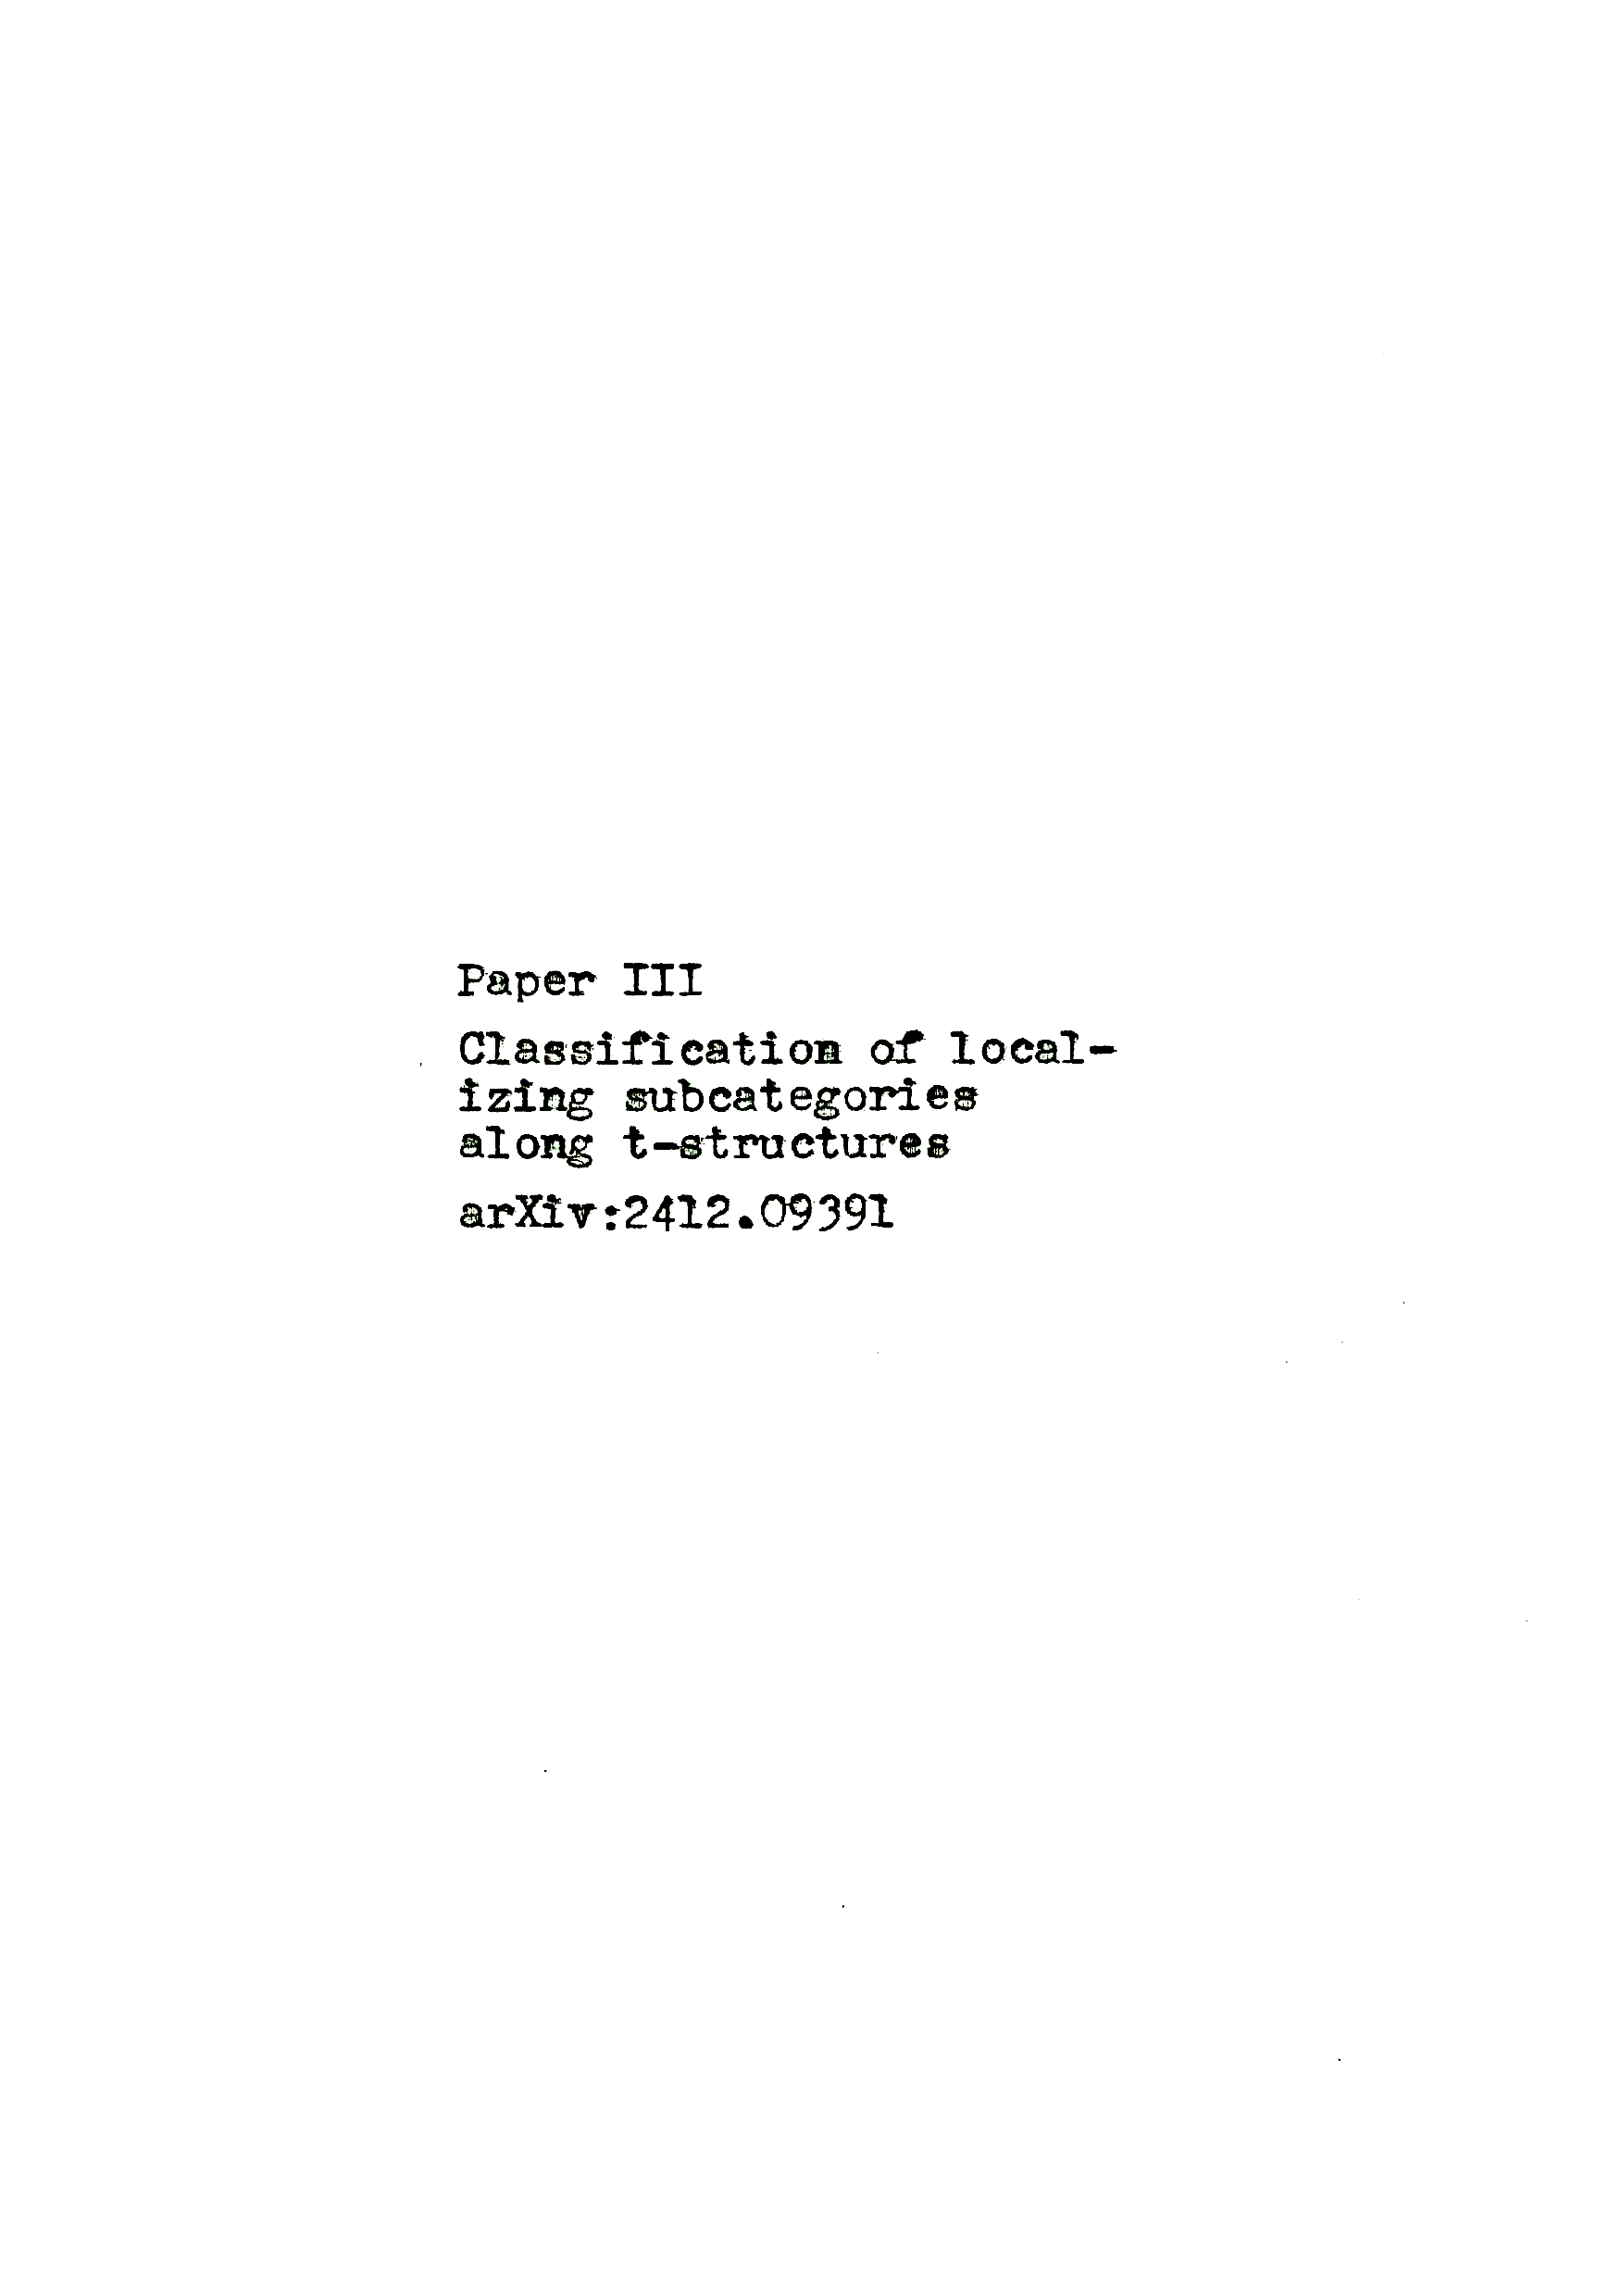
\includegraphics[%
clip,
width=1.05\paperwidth,
height=1.05\paperheight
]{chaptertitles/paper3.png}};

\clearpage


\newpage
\tikz[remember picture,overlay]\node[opacity=1,inner sep=0pt] at (current page.center)%
{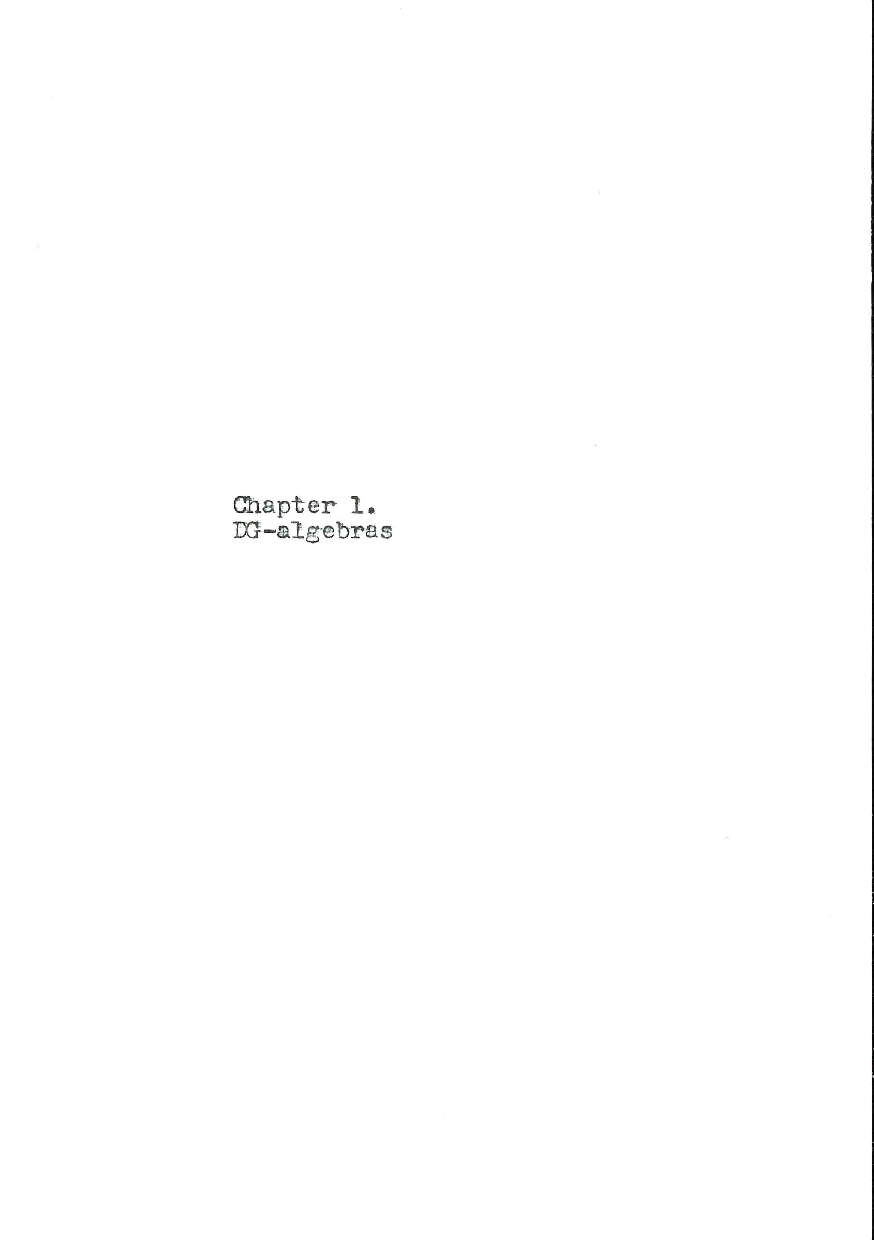
\includegraphics[%
clip,
width=1.05\paperwidth,
height=1.05\paperheight
]{chaptertitles/ch1.pdf}};

\clearpage


\subsection*{Description}

The main result of the third paper concerns a connection between three different related mathematical worlds, called the stable, the prestable and the abelian world. These three worlds are all connected by a mathematical concept called a $t$-structure. One could think of this setup as follows: in the stable world we have an infinite list of things, labeled by every positive and negative whole number. In the prestable world we only have things labeled by positive numbers, which still gives us infinitely many things, but only in one direction. In the abelian world we have only the part labeled by $0$---the only part right between the positive and the negative. The $t$-structure allows us to remove all of the information in any degree. For example, it can first remove all negative numbers, and then all positive numbers, leaving us only with $0$. This is precisely how it connects the stable, the prestable and the abelian worlds. I have tried to signify this passing in the drawing, where one the left we have free flowing information in all directions, while in the middle half of it is restricted in one direction. In the final rightmost part, information is restricted in both directions, leaving us only with straight lines---no geometry, no topology. 

The colors again have no mathematical meaning, and are there only to add visual interst, and to connect to the colors of the papers. 

\newpage

\thispagestyle{plain}
\section*{}
\addcontentsline{toc}{section}{Limerick III}

\vspace*{7cm}


\begin{verse}
    \hspace{8em}Let $\C$ be stable with a $t$ \\
    \vspace{5pt}
    \hspace{8em}---as nice as it needs to be. \\
    \vspace{5pt}
    \hspace{8em}If the heart has a localization, \\
    \vspace{5pt}
    \hspace{8em}then I have a declaration: \\
    \vspace{5pt}
    \hspace{8em}There is a unique $\pi$-exact lift to $\C$. 

    %\hspace{\fill}-- Torgeir Aambø
\end{verse}\newpage



\vspace*{2em}

{\par\centering {\Large \textbf{Abstract:}}\par}
\vspace{-2em}
\rule[-11pt]{\textwidth}{1pt}
\rule{\textwidth}{0.5pt}
    
We study the interplay between localizing subcategories in a stable $\infty$-category $\C$ with $t$-structure $(\C\geqz, \C\leqz)$, the prestable $\infty$-category $\C\geqz$ and the abelian category $\C^\heart$. We prove that weak localizing subcategories of $\C^\heart$ are in bijection with the localizing subcategories of $\C$ where object-containment can be checked on the heart. This generalizes similar known correspondences for noetherian rings and bounded $t$-structures. We also prove that this restricts to a bijection between localizing subcategories of $\C^\heart$, and localizing subcategories of $\C$ that are kernels of $t$-exact functors---lifting Lurie's correspondence between localizing subcategories in $\C\geqz$ and $\C^\heart$ to the stable category $\C$. 

\rule{\textwidth}{0.5pt}
\rule[11pt]{\textwidth}{1pt}

{\setstretch{0.5}
\printcontents[chapters]{p}{1}{}
}
\vspace{\fill}
\newpage


\section{Introduction}

The concept of a $t$-structure on a triangulated category was introduced in \cite{beilinson-bernstein-deligne_1983}, and in a way axiomatizes the concept of taking the homology of a chain complex in the derived category of a ring. Most interesting triangulated categories arise as the homotopy category of a stable $\infty$-category, and the concept of a $t$-structure lifts to this setting. Having a $t$-structure allows us to naturally compare features of a stable $\infty$-category $\C$ to features of an abelian category $\C^\heart$, called the heart of the given $t$-structure. 

In order to understand the internal structure of a stable $\infty$-category, is its important to understand its \emph{localizing subcategories}. A full subcategory is called localizing if it is a stable full subcategory closed under colimits. The goal of this paper is to classify the localizing subcategories of $\C$ that interact well with $t$-structures. These are the localizing subcategories $\L\subseteq \C$ that inherit a $t$-structure, and you can check if an object $X$ is in $\L$ by checking whether $\pi_n^\heart X\in \L^\heart$. We call these the \emph{$\pi$-stable localizing subcategories}.

We want to compare these localizing subcategories of $\C$ to subcategories of $\C^\heart$. The abelian analog of localizing subcategories of a stable $\infty$-category, are the \emph{weak Serre subcategories} closed under coproducts. We call these the \emph{weak localizing subcategories}. Our first main result is the following classification of $\pi$-stable localizing subcategories in $\C$ via the heart construction. This generalizes a similar correspondence for commutative noetherian rings, due to Takahashi---see \cite{takahashi_2009} or \cref{ch3:cor:takahashi-weak-localizing}. 

\begin{introthm}[\cref{ch3:thm:premain}]
    \label{ch3:thm:A}
    If $\C$ is a stable $\infty$-category right complete $t$-structure compatible with filtered colimits, then the map $\L\longmapsto \L^\heart$ gives a one-to-one correspondence between $\pi$-stable localizing subcategories of $\C$ and weak localizing subcategories in $\C^\heart$.
\end{introthm}

The above theorem also holds when we exclude the existence of coproducts, giving a one-to-one correspondence between $\pi$-stable thick subcategories of $\C$ and weak Serre subcategories of $\C^\heart$. This generalizes the similar result of Zhang--Cai (\cite{zhang-cai_2017}) to the setting of unbounded $t$-structures, see \cref{ch3:prop:classification-weak-serre} and \cref{ch3:cor:classification-weak-serre-bounded}. 

There is also a notion of \emph{localizing subcategories} of the abelian category $\C^\heart$---being Serre subcategories closed under arbitrary coproducts---and we want to understand how the correspondence in \cref{ch3:thm:A} can be restricted to this setting. In order to do this we use the bridge between stable $\infty$-categories with a $t$-structure and prestable $\infty$-categories, as developed mainly by Lurie in \cite[App. C]{lurie_SAG}. A prestable $\infty$-category acts as the connected part of the $t$-structure, denoted $\C\geqz$, and they allow us to study $t$-structures on $\C$ indirectly, without carrying around extra data. 

Lurie introduced the notion of localizing subcategories of the prestable $\infty$-category $\C\geqz$, which more closely mimics the construction of localizing subcategories of abelian categories. The prestable analog of a $\pi$-stable localizing subcategory are the \emph{separating localizing subcategories}. Lurie classified the separating localizing subcategories of $\C\geqz$ in \cite[C.5.2.7]{lurie_SAG}, by proving that there is a one-to-one correspondence
\[\separating \simeq \ablocalizing.\]
Our second main theorem provides an extension of this correspondence to the stable $\infty$-category $\C$, allowing us to strengthen \cref{ch3:thm:A} to non-weak localizing sucategories. This interacts well with existing classifications of localizing subcategories in modules over noetherian rings and quasicoherent sheaves on noetherian schemes. 

% In order to avoid confusion we follow \cite{hovey-strickland_2005a} and \cite{barthel-heard_2018} in using the name \emph{hereditary torsion theories} instead of localizing subcategories of the heart $\C^\heart$. These two notions are equivalent in Grothendieck abelian categories, hence a natural alternative. 

\begin{introthm}[{\cref{ch3:thm:main}}]
    \label{ch3:thm:B}
    Let $\C$ be a stable category with a $t$-structure. If the $t$-structure is right complete and compatible with filtered colimits, then the map $\L\longmapsto \L^\heart$ gives a one-to-one correspondence between localizing subcategories of $\C^\heart$, and $\pi$-stable localizing subcategories of $\C$ that are kernels of a $t$-exact localization.
\end{introthm}

Note that any stable $\infty$-category is prestable, hence the above result might at first glance seem to follow trivially from Luries's classification. But, any separating localizing subcategory of a stable $\infty$-category $\C$, viewed as a prestable one, is the whole category $\C$ by \cite[C.1.2.14, C.5.2.4]{lurie_SAG}. This means that the stable situation needs its own separate treatment, hence the existence of the current paper. 

The results of the paper can be summarized in the following diagram, showcasing the bijections ($\simeq$) and the inclusions ($\subseteq$) between the different types of subcategories. 


\begin{center}
    \adjustbox{scale=0.98,center}{
    \begin{tikzcd}
        \tcompatible 
        \arrow[rrd, "(-)^\heart"]
        &&\\
        \pistable 
        \arrow[rr, "\simeq"] 
        \arrow[u, hook, "\subseteq", swap] 
        && 
        \weaklocalizing  
        \\
        \piexact 
        \arrow[r, "\simeq"] 
        \arrow[d, hook, "\subseteq"]
        \arrow[u, hook, "\subseteq", swap] 
        & 
        \separating 
        \arrow[r, "\simeq"]
        \arrow[d, hook, "\subseteq"]
        & 
        \ablocalizing
        \arrow[u, hook, "\subseteq", swap]
        \\
        \texact 
        \arrow[r, "(-)\geqz"]
        & 
        \prlocalizing 
        \arrow[ru, "(-)\leqz", swap] 
        &                                
        \end{tikzcd}
    }
\end{center}




\textbf{Linear overview:} We start \cref{ch3:sec:prestable-and-stable-categories} with some recollections on $t$-structures, prestable $\infty$-categories, and their interactions, before we introduce the notion of localizing subcategories in \cref{ch3:ssec:localizing-subcategories}. We then study some further interactions between these, which we use to prove \cref{ch3:thm:A} in \cref{ch3:ssec:classificartion-weak-localizing} and \cref{ch3:thm:B} in \cref{ch3:ssec:classificartion-localizing}. We finish the paper by looking at some consequences and applications of our results. 

\textbf{Conventions:} We will work in the setting of $\infty$-categories, as developed by Lurie in \cite{lurie_09} and \cite{Lurie_HA}. We will restrict our attention to presentable stable $\infty$-categories, which we will just call \emph{stable categories}. Given a stable category $\C$ with a nice $t$-structure, its associated prestable category will be denoted $\C\geqz$ and its heart by $\C^\heart$. We assume all $t$-structures to be accessible.

\textbf{Acknowledgements:} We wish to thank Drew Heard and Marius Nielsen for helpful conversations. This work was partially finished during the authors visit to the GeoTop center at the University of Copenhagen, which we gratefully thank for their hospitality. This work was supported by grant number TMS2020TMT02 from the Trond Mohn Foundation.    

\section{Prestable and stable categories}
\label{ch3:sec:prestable-and-stable-categories}

For the rest of the paper we fix a stable category $\C$. We wish to equip this with a $t$-structure, which will allow us to always have a comparison from $\C$ to an abelian category. The main reference for $t$-structures in this setting is \cite[Sec 1.2.1]{Lurie_HA}. Note that, as opposed to much of the homological algebra literature, we follow Lurie's homological indexing convention.  

\begin{definition}
    \index{t-structure}
    A \emph{$t$-structure} on $\C$ is a pair of full subcategories $(\C\geqz, \C\leqz)$ such that:
    \begin{enumerate}
        \item The mapping space $\Map_\C(X,Y[-1])\simeq 0$ for all $X\in \C\geqz$ and $Y\in \C\leqz$;
        \item There are inclusions $\C\geqz[1]\subseteq \C\geqz$ and $\C\leqz[-1]\subseteq \C\leqz$;
        \item For any $Y\in \C$ there is a fiber sequence $X\to Y\to Z$ such that $X\in \C\geqz$ and $Z[1]\in \C\leqz$. 
    \end{enumerate} 
\end{definition}

This is equivalent to choosing a $t$-structure on the homotopy category $h\C$, which is a triangulated category. Hence the contents of this paper should be equally useful to those familiar with $t$-structures on triangulated categories. 

We will assume all $t$-structures to be accessible, in the sense that the connected part $\C\geqz$ is presentable. By \cite[1.2.16]{Lurie_HA} the inclusions $\C\geqz\to \C$ and $\C\leqz\to \C$ have a right adjoint $\tau\geqz$ and a left adjoint $\tau\leqz$ respectively. We denote $\C\geqn := \C\geqz[n]$ and $\C\leqn := \C\leqz[n]$. 

\begin{definition}
    \index{t-structure!Heart}
    The heart of a $t$-structure $(\C\geqz, \C\leqz)$ on $\C$ is defined as the full subcategory $\C^\heart := \C\geqz\cap\C\leqz$.
\end{definition}

The heart $\C^\heart$ is always equivalent to the nerve of its homotopy category $h\C^\heart$, which was proven in \cite{beilinson-bernstein-deligne_1983} to be an abelian category. It is standard to follow \cite[1.2.1.12]{Lurie_HA} and identify the two. 

\begin{definition}
    \index{t-structure!Homotopy groups}
    The composite functor 
    \[\tau\geqz\circ\tau\leqz\simeq\tau\leqz\circ\tau\geqz \: \C\to \C^\heart\]
    is denoted by $\pi_0^\heart$ and its composition with the shift functor $X\to X[-n]$ by $\pi_n^\heart$. These are called the \emph{heart-valued homotopy groups} of $X$. 
\end{definition}

The last definition we will need, before going on to prestable categories is the following niceness condition. 

\begin{definition}
    \index{t-structure!Compatible with filtered colimits}
    A $t$-structure $(\C\geqz, \C\leqz)$ on a stable category $\C$ is said to be \emph{compatible with filtered colimits} if $\C\leqz$ is closed under all filtered colimits in $\C$. 
\end{definition}

\begin{remark}
    This ensures, among other things, that the functor $\pi_0^\heart$ preserves filtered colimits. 
\end{remark}

We now recall the notion of prestable $\infty$-categories, which, similarly to the stable $\infty$-categories, we will simply call \emph{prestable categories}. The theory of prestable categories was developed by Lurie in \cite[App. C]{lurie_SAG}, and has since been applied in a varied range of areas. We define these as follows. 

\begin{definition}
    \index{Prestable $\infty$-category}
    An $\infty$-category $\D$ is \emph{prestable} if there exists a stable category $\C$ with a $t$-structure $(\C\geqz, \C\leqz)$, such that $\D\simeq \C\geqz$.
\end{definition}

\begin{remark}
    This is not the most general, nor the standard, definition of a prestable category---see \cite[C.1.2.1]{lurie_SAG}---but by \cite[C.1.2.9]{lurie_SAG} the above definition describes all prestable categories admitting finite limits, hence it is not a very severe restriction. The category $\D$ is also not unique, see \cite[C.1.2.10]{lurie_SAG}, but we will mostly focus on the choice 
    \[\D=\Sp(\C\geqz) = \colim (\cdots\overset{\Omega}\to\C\geqz\overset{\Omega}\to\C\geqz).\]
\end{remark}

Since we will discuss both stable and prestable categories, and their interactions, we will try to consequently denote prestable categories by $\C\geqz$ and stable categories by $\C$. 

\begin{remark}
    \label{ch3:rm:stable-is-prestable}
    Any stable category $\C$ is prestable, as seen by choosing the trivial $t$-structure $(\C,0)$. This is both a blessing, as it allows us to talk about both in a common language, and a curse, as using common language can be rather confusing when trying to study their interactions.
\end{remark}

We will restrict our attention to Grothendieck prestable categories, which intuitively are the prestable categories that work well with colimits. There are numerous different equivalent definitions of these, see \cite[C.1.4.1]{lurie_SAG}, but the one best related to the above definition of a prestable category is the following. 

\begin{definition}
    \index{Prestable $\infty$-category!Grothendieck}
    A prestable category $\C\geqz$ is \emph{Grothendieck} if the $t$-structure on its associated stable category $\C$ is compatible with filtered colimits. 
\end{definition}

The following example is perhaps the main reason for the naming convention.

\begin{example}
    \index{Grothendieck abelian}
    For any Grothendieck abelian category $\A$, the derived category $\Der(\A)$ has a natural $t$-structure with heart $\A$. The connected component $\Der(\A)\geqz$, which consists of complexes $X_\bullet$ such that $H_i(X_\bullet) = 0$ for $i<0$ is a Grothendieck prestable category.  
\end{example}

\begin{example}
    Let $X$ be a noetherian scheme. The derived category of all $\O_X$-modules has a full subcategory consisting of the complexes with quasi-coherent homology. which we denote by $\Der_{qc}(X)$. There is a natural $t$-structure on $\Der_{qc}(X)$, defined similarly to the natural $t$-structure on $\Der(R)$, and the connected component $\Der_{qc}(X)\geqz$ is a Grothendieck prestable category. 
\end{example}

We also have some examples showing up in stable homotopy theory. 

\begin{example}
    \index{Spectra}
    Let $\Sp$ be the stable $\infty$-category of spectra. This has a natural $t$-structure with heart $\Ab$. The connected component $\Sp\geqz$, consisting of connective spectra, is a Grothendieck prestable category. 
\end{example}

\begin{example}
    \index{Synthetic spectra}
    Important for modern homotopy theory is the category of $E$-based synthetic spectra $\SynE$ for some Landweber exact homology theory $E$, see \cite{pstragowski_2022}. This has a naturally occurring $t$-structure with heart $\ComodE$, and its connected component $\Syn_{E, \geq 0}$ is Grothendieck prestable. This example is one of our main motivations for this work, and we plan to study the applications of the contents in this paper to synthetic spectra in future work. 
\end{example}

% \begin{construction}
%     Let $\C\geqz$ and $\D\geqz$ be Grothendieck prestable categories. By \cite[C.4.2.1]{lurie_SAG} the tensor product $\C\geqz\otimes \D\geqz$ in $\PrL$ is again Grothendieck prestable. Hence we get an induced symmetric monoidal structure on the category $\Groth$ of Grothendieck prestable categories. We will call categories $\C\geqz\in \CAlg(\Groth)$ symmetric monoidal Grothendieck prestable categories. Since we formed the tensor in $\PrL$ the tensor product in a symmetric monoidal Grothendieck prestable category still preserves colimits separately in each variable.  
% \end{construction}

% \begin{example}
%     Let $\C\geqz \in \CAlg(\Groth)$ be a symmetric monoidal Grothendieck prestable category and $A \in \CAlg(\C\geqz)$. Then $\Mod_A(\C\geqz)$ is Grothendieck prestable. This is a consequence of \cite[10.4.3.1]{lurie_SAG} -- see also \cite[2.4.5]{stefanich_2023}.
% \end{example}

\begin{remark}
    \label{ch3:rm:stable-is-grothendieck-prestable}
    \index{Compactly generated}
    If the prestable category $\C\geqz$ is compactly generated, then it is automatically Grothendieck, see \cite[C.1.4.4]{lurie_SAG}. A stable $\infty$-category $\C$ is, as mentioned above, also prestable. It is in fact Grothendieck if and only if it is presentable. 
\end{remark}

\begin{definition}
    \index{t-structure!Right complete}
    We say a $t$-structure on a stable category $\C$ is \emph{right complete} if the natural functor 
    \[\displaystyle {\underset{n}\colim} \C_{\geq -n} \overset{\simeq}\to \C\] 
    is an equivalence. 
\end{definition}

\begin{remark}
    \label{ch3:rm:grothendieck-iff-right-complete-and-colims}
    \index{Stabilization}
    For any Grothendieck prestable category $\C\geqz$ the functor $\Sp(-)$, sending $\C\geqz$ to its stabilization, $\Sp(\C\geqz)$, provides a one-to-one correspondence between Grothendieck prestable categories and stable categories equipped with a right complete $t$-structure compatible with filtered colimits. This is one of the main reasons to study prestable categories, as being prestable is a property, while having a $t$-structure is extra structure. 
\end{remark}

% \begin{remark}
%     If $\C$ is a stable category with a $t$-structure compatible with filtered colimits, then the heart-valued homotopy groups functors $\pi_n^\heart$ preserve filtered colimits. 
% \end{remark}













\subsection{Bridging the gap}

In this section we study the passage from stable to prestable and vice versa, particularly focusing on when they determine each other. 

If $\C$ is a stable category with a right complete $t$-structure $(\C\geqz, \C\leqz)$, then we can reconstruct it from its connected component. 

\begin{lemma}[{\cite[C.1.2.10]{lurie_SAG}}]
    \label{ch3:lm:right-complete-then-equiv-to-sp}
    Let $\C$ be a stable category. If $\C$ has a right complete $t$-structure, then there is an equivalence $\Sp(\C\geqz)\simeq \C$. 
\end{lemma}

This fact also extends to equivalences of categories, as proven by Antieau. 

\begin{lemma}[{\cite[6.1]{antieau_2021}}]
    \label{ch3:lm:if-prestable-equiv-then-stable-equiv}
    Let $\C$ and $\D$ be stable categories equipped with right complete $t$-structures. If $\C\geqz\simeq \D\geqz$, then also $\C\simeq \D$. 
\end{lemma}

We also have a natural converse statement: if we have an equivalence of stable categories $\C\simeq \D$, that is compatible with the $t$-structures, then we get an induced equivalence on the connected components $\C\geqz\simeq \D\geqz$. The precise definition of being compatible with the $t$-structures is as follows. 

\begin{definition}
    \index{t-exact functor}
    Let $\C, \D$ be stable categories with $t$-structures. An exact functor $F\:\C\to\D$ is \emph{right $t$-exact} if $F(\C\geqz)\subseteq \D\geqz$. The notion of \emph{left $t$-exactness} is defined similarly. If $F$ is both left and right $t$-exact, we say that it is a \emph{$t$-exact functor}. 
\end{definition}

\begin{remark}
    This convention might seem wrong to readers with a background in homological algebra, as the role of left and right $t$-exact functors are usually the opposite. This flip is a consequence of using the homological indexing convention rather than cohomological indexing. 
\end{remark}

\begin{lemma}
    Let $\C$ and $\D$ be stable categories with $t$-structures. If $F\:\C\to\D$ is a right $t$-exact functor, then we have an induced functor of prestable categories $F\geqz\:\C\geqz\to\D\geqz$. If $F$ is an equivalence, then so is $F\geqz$. 
\end{lemma}

For the rest of the paper we will use the following terminology. 

\begin{definition}
    \index{Presentable $\infty$-category!t-stable}
    A \emph{$t$-stable category} is a stable category $\C$ together with a choice of a right complete $t$-structure compatible with filtered colimits. 
\end{definition}

\begin{example}
    All of the examples mentioned earlier---being $\Der(R)$, $\Der_{qc}(X)$, $\Sp$ and $\SynE$---are $t$-stable categories. 
\end{example}

\begin{remark}
    Let $\C$ be a $t$-stable category. By definition we have that the connective part, $\C\geqz$, is a Grothendieck prestable category, and that the heart $\C^\heart$ is a Grothendieck abelian category. Hence $t$-stable categories serve as a natural place to study the interactions between these three types of categories. 
\end{remark}

\begin{remark}
    In \cite[Section C.3.1]{lurie_SAG} Lurie constructs a category of $t$-stable categories. If we denote this by $t\Cat$ then the contents of \cref{ch3:rm:grothendieck-iff-right-complete-and-colims} can be described as an adjoint pair of equivalences
    \begin{center}
        \begin{tikzcd}
            \Groth \arrow[r, "\Sp(-)", yshift=2pt] & t\Cat \arrow[l, "(-)\geqz", yshift=-2pt].
        \end{tikzcd}
    \end{center}
    This should, however, be viewed as a heuristic rather than a very precise statement, as the right hand category is a bit tricky to define. 
\end{remark}







\subsection{Localizing subcategories}
\label{ch3:ssec:localizing-subcategories}

We now turn our attention to localizing subcategories. As we are working in three interconnected settings---stable, prestable and abelian---and all settings use the same terminology, we feel that this section is very ripe for confusions to occur. In an attempt to clarify which setting we are in, we will usually refer to localizing subcategories of stable categories as \emph{stable localizing subcategories}, localizing subcategories of prestable categories as \emph{prestable localizing subcategories} and localizing subcategories of abelian categories as \emph{abelian localizing subcategories}. We will, however, sometimes omit the categorical prefix when we feel that it is clear from context. 

\begin{definition}
    \index{Thick subcategory}
    \index{Localizing subcategory!Stable}
    Let $\C$ be a stable category. A full subcategory $\L\subseteq \C$ is said to be \emph{thick} if it is a full stable subcategory closed under finite colimits. In particular, it is closed under extensions and desuspensions. We say $\L$ is a \emph{stable localizing subcategory} if it is thick and closed under filtered colimits. 
\end{definition}

Stable localizing subcategories are uniquely determined by localization functors on $\C$, hence their name. This is a standard fact about localizations, but we include a sketch of the proof for convenience. 

\begin{lemma}
    \index{Localization}
    A full subcategory $\L$ of a stable category $\C$, is a stable localizing subcategory if and only if there is a stable category $\D$, and an exact localization $L\:\C\to\D$, such that $\L$ is the kernel of $L$. 
\end{lemma}
\begin{proof}
    Let $\L$ be an arbitrary localizing subcategory of $\C$. The right-orthogonal complement\index{Right orthogonal complement} of $\L$, denoted
    \[\L^\perp = \{C\in \C \mid \Hom(X, C)\simeq 0, \forall X\in \C\},\]
    is closed under all limits in $\C$, meaning that the fully faithful inclusion $\L^\perp \hookrightarrow \C$ has a left adjoint $L$. This is an exact localization of stable $\infty$-categories, and the kernel is precisely $\L$. 
    
    For the converse, assume we are given an exact localization functor $L\: \C\to \D$ such that $\L = \Ker L$. Then $\L$ is a stable category by the exactness of $L$, which is in addition closed under colimits as $L$ preserves these by being a left adjoint. 
\end{proof}

% The definition of a localizing subcategory of a prestable category is meant to generalize this slightly. Since all stable categories are prestable, we want a localizing subcategory $\L$ of a prestable category $\C\geqz$ to coincide with the above definition wenever $\C$ is stable. 

The definition of a localizing subcategory of a prestable category is very similar in nature to its stable brethren, but there is a slight variation. 

\begin{definition}
    \index{Sub-object}
    Let $\C\geqz$ be a Grothendieck prestable category and $C$ an object in $\C$. Another object $C'\in \C$ is said to be a sub-object of $C$ if there is a map $f\: C'\to C$ with $ \Cofib(f)\in \C^\heart$. 
\end{definition}

\begin{remark}
    For Grothendieck prestable categories, this is equivalent to the assertion that $C'$ is a $(-1)$-truncated object in $\C_{/C}$ via the map $f$, which is the more standard definition of being a sub-object---see \cite[C.2.3.4]{lurie_SAG}
\end{remark}

\begin{definition}[{\cite[C.2.3.3]{lurie_SAG}}]
    \index{Localizing subcategory!Prestable}
    Let $\C\geqz$ be a Grothendieck prestable category. A full subcategory $\L\geqz\subseteq \C\geqz$ is a \emph{prestable localizing subcategory} if it is accessible and closed under coproducts, cofiber sequences and sub-objects. 
\end{definition}

\begin{remark}
    \label{ch3:rm:prestable-localizing-is-Grothendieck}
    If $\C\geqz$ is Grothendieck prestable, then any prestable localizing subcategory $\L\geqz$ is by \cite[C.5.2.1]{lurie_SAG} itself a Grothendieck prestable category. This means, in particular, that $\L\geqz$ is the connected part of a colimit-compatible $t$-structure on a stable category, hence using the notation $\L\geqz$ is not abusive. 
\end{remark}

\begin{remark}
    \label{ch3:rm:prestable-localizing-in-stable-then-stable-localizing}
    Recall from \cref{ch3:rm:stable-is-prestable} that any stable category $\C$ can be treated as a prestable category. By \cite[C.2.3.6]{lurie_SAG} a full subcategory $\L$ of $\C$ is a prestable localizing subcategory if and only if it is a stable localizing subcategory. 
\end{remark}

As in the stable situation we have a description of prestable localizing subcategories via localization functors. 

\begin{proposition}[{\cite[C.2.3.8]{lurie_SAG}}]
    \label{ch3:prop:Lurie-prestable-localizing-left-exact-functor}
    A full subcategory $\L\geqz$ of a Grothendieck prestable category $\C\geqz$ is localizing if and only if there is a Grothendieck prestable category $\D\geqz$, and left exact localization $L\:\C\geqz\to\D\geqz$, such that $\L\geqz$ is the kernel of $L$. 
\end{proposition}


As prestable localizing subcategories are again prestable, we know that there is some stable category with a $t$-structure presenting it as its connected component. The prestable localizing subcategories hence naturally encodes a sort of induced $t$-structure. This does not happen automatically for stable categories, hence we need to make some additional requirements in order to successfully move between the prestable and stable situation. 

\begin{definition}
    \label{ch3:def:t-stable-localizing-subcategory}
    \index{Localizing subcategory!t-stable}
    Let $\C$ be a $t$-stable category. A full subcategory $\L\subseteq \C$ is said to be a \emph{$t$-stable localizing subcategory} if it is localizing, and for any $X\in \L$ we have $\tau\geqz X\in \L$ and $\tau\leqz X\in \L$. 
\end{definition}

\begin{remark}
    We hope that using both the names $t$-stable categories and $t$-stable localizing subcategories does not cause confusion. We decided to use this terminology, as a $t$-stable localizing subcategory is itself a $t$-stable category, as we will see in \cref{ch3:lm:localizing-inherits-completeness-and-colimits}. 
\end{remark}

\begin{remark}
    Let $\L$ be a $t$-stable localizing subcategory of $\C$. As localizing subcategories are stable under (de)suspension, this means that also all $\tau\geqn X$ and $\tau\leqn$ lie in $\L$ for all $n$. In particular, the homotopy groups $\pi_n^\heart X$ lie in $\L$ for all $n$. 
\end{remark}

\begin{remark}
    \label{ch3:rm:t-stable-truncation-homotopy-the-same-functors}
    This definition is motivated by \cite[1.3.19]{beilinson-bernstein-deligne_1983}, where the authors prove that such a full subcategory inherits a $t$-structure given by 
    \[(\L\geqz, \L\leqz) = (\C\geqz\cap \L, \C\leqz\cap \L)\]
    with heart $\C^\heart\cap \L$. In other words, a $t$-stable localizing subcategory has a ``sub $t$-structure'', such that the inclusion is $t$-exact. In particular, the truncation functors $\tau\geqn$ and $\tau\leqn$ are the same as those in $\C$, hence also the homotopy group functors $\pi_n^\heart$ are the same in $\C$ and $\L$. 
\end{remark}

% This fact can be made slightly more general, as the following lemma shows. 

% \begin{lemma}[{\cite[Lemma 2.16]{antieau-gepner-heller_2019}}]
%     If $F\:\C\to\D$ is a fully faithful $t$-exact functor of $t$-stable categories, then the induced functor
%     \[F^\heart \: \C^\heart \to \D^\heart \cap \C\]
%     is an exact equivalence of abelian categories. 
% \end{lemma}

We will from now on assume that a $t$-stable localizing subcategory is equipped with the above $t$-structure. 

\begin{proposition}
    \label{ch3:prop:induced-t-structure-on-stable-localizing}
    Let $\C$ be a stable category with a right complete $t$-structure and let $\L\subseteq \C$ be a localizing subcategory. If $\L$ is $t$-stable, then the induced $t$-structure on $\L$ is right complete.  
\end{proposition}
\begin{proof}
    This follows immediately from the fact that the truncation functors are the same as in $\C$, and that colimits in $\L$ are the same as those in $\C$. 
\end{proof}

The last thing to introduce in this section are the abelian analogs of the above definitions. 

\begin{definition}
    \index{Serre subcategory!Weak}
    \index{Localizing subcategory!Abelian weak}
    A full subcategory $\T$ of a Grothendieck abelian category $\A$ is called a \emph{weak Serre subcategory}, if for any exact sequence 
    \[A_1 \to A_2 \to A_3 \to A_4 \to A_5\]
    in $\A$ such that $A_1, A_2, A_4, A_5$ are all in $\T$, then also $A_3 \in \T$. It is an \emph{abelian weak localizing subcategory} if it is a weak Serre subcategory closed under arbitrary coproducts. 
\end{definition}

\begin{remark}
    A full subcategory is a weak Serre subcategory if it is closed under kernels, cokernels and extensions. In particular it is an abelian subcategory, and the fully faithful inclusion functor $\T\hookrightarrow \A$ is exact. 
\end{remark}

\begin{definition}
    \index{Serre subcategory}
    \index{Localizing subcategory!Abelian}
    A full subcategory $\T$ of a Grothendieck abelian category $\A$ is called a \emph{Serre subcategory} if for any short exact sequence 
    \[0\to A\to B\to C\to 0\]
    in $\A$, we have $B\in \T$ if and only if $A, C \in \T$. It is an \emph{abelian localizing subcategory} if it is a Serre subcategory closed under arbitrary coproducts. 
\end{definition}

\begin{remark}
    A full subcategory is a Serre subcategory if it is closed under sub-objects, quotients and extensions. This means that all Serre subcategories are weak Serre subcategories, and that all abelian localizing subcategories are abelian weak localizing subcategories. In particular they are all abelian subcategories with exact inclusions into $\A$. 
\end{remark}

\begin{remark}
    Weak Serre subcategories seem to also be called \emph{thick} or \emph{wide} subcategories in the homological algebra literature. But, to make the connection with abelian localizing subcategories clearer we chose to use this terminology. 
\end{remark}

As one perhaps should expect at this point, Abelian localizing subcategories are also determined by localization functors---as above, so below. 

\begin{proposition}[{\cite[C.5.1.1, C.5.1.6]{lurie_SAG}}]
    \label{ch3:prop:abelian-localizing-iff-kernel-of-localization}
    \index{Localization}
    A full subcategory $\T\subseteq \A$, where $\A$ is Grothendieck abelian, is an abelian localizing subcategory if and only if there is an exact localization functor $L\:\A\to \B$, such that $\B$ is a Grothendieck abelian category and $\T$ is the kernel of $L$. 
\end{proposition}

% Later in the paper we will need the following technical lemma, which allows us to define weak Serre subcategories via short exact sequences instead of $5$-term ones. 

% \begin{lemma}
%     If $\T\subseteq \A$ is a full subcategory, then $\T$ is a weak Serre subcategory if and only if for any short exact sequence 
%     \[0 \to A \to B \to C \to 0\]
%     in $\A$ such that two of the three objects $A, B, C$ are in $\T$, then also the last one is. 
% \end{lemma}





\subsection{Stable and prestable comparisons}

The first thing we need is to be able to recognize stable localizing subcategories by their connected part, as we did for stable categories in \cref{ch3:lm:right-complete-then-equiv-to-sp}. 

\begin{corollary}
    \label{ch3:cor:t-stable-implies-equiv-to-sp}
    If $\C$ is a stable category with a right complete $t$-structure and $\L$ a $t$-stable localizing subcategory, then there is an equivalence $\L\simeq \Sp(\L\geqz)$. 
\end{corollary}
\begin{proof}
    This follows directly from \cref{ch3:prop:induced-t-structure-on-stable-localizing} and \cref{ch3:lm:right-complete-then-equiv-to-sp}.
\end{proof}

Using this we can increase the strength of \cref{ch3:prop:induced-t-structure-on-stable-localizing} by also incorporating compatibility with filtered colimits. Recall that we use the name $t$-stable category for a stable category with a right complete $t$-structure compatible with filtered colimits. 

\begin{lemma}
    \label{ch3:lm:localizing-inherits-completeness-and-colimits}
    Let $\C$ be a $t$-stable category and $\L$ a localizing subcategory. If $\L$ is $t$-stable, then $\L$ is itself a $t$-stable category. 
\end{lemma}
\begin{proof}
    By \cref{ch3:prop:induced-t-structure-on-stable-localizing} we know that the induced $t$-structure on $\L$ is right complete. By \cite[C.5.2.1(1)]{lurie_SAG} $\L\geqz$ is Grothendieck prestable, hence the $t$-structure on its stabilization $\Sp(\L\geqz)$ is compatible with filtered colimits by definition, see \cite[C.1.4.1]{lurie_SAG}. This stabilization is by \cref{ch3:cor:t-stable-implies-equiv-to-sp} equivalent to $\L$, completing the proof. 
\end{proof}

% \begin{remark}
%     Notice that the above holds immediately if $\L$ is compactly generated, as then the left exact right adjoint to the inclusion $\Gamma\colon \C\to\L$ preserves colimits. 
% \end{remark}

% We now want to provide an alternative view-point for $t$-stable localizing subcategories that is based on localization functors. 

% \begin{lemma}
%     \label{ch3:lm:t-stable-iff-t-exact}
%     Let $\L\subseteq \C$ be a $t$-stable stable localizing subcategory. Then there is a $t$-exact localization $L\:\C\to\D$ such that $\L$ is the full subcategory spanned by the $L$-acyclic objects. 
% \end{lemma}
% \begin{proof}
%     Since $L$ is a stable localizing subcategory, there exists a localization $L$ such that $\L$ is the full subcategory spanned by the $L$-acyclics. The functor $L$ is given by the left adjoint to the equivalence $\D\simeq \C[S^{-1}]\subseteq \C$, where $S$ is the class of maps $f\: X\to Y$ in $\C$ such that $\fib(f)\in \L$. We claim that $\L$ is $t$-stable if and only if $L$ is $t$-exact. 
%     \todo[inline]{finish}
% \end{proof}

% We will use this, together with the following lemma by Lurie, to prove that the connected part of a $t$-stable stable localizing subcategory is a prestable localizing subcategory. 

% We now prove our first results towards the wanted correspondences in \cref{ch3:thm:A} and \cref{ch3:thm:B}. 

% \begin{lemma}
%     \label{ch3:lm:stable-localizing-then-prestable-localizing}
%     If $\L\subseteq \C$ is a $t$-stable stable localizing subcategory of a $t$-stable category $\C$, then the category $\L\geqz$ is a prestable localizing subcategory of $\C\geqz$. 
% \end{lemma}
% \begin{proof}
%     The category $\L$ is itself $t$-stable by \cref{ch3:lm:localizing-inherits-completeness-and-colimits}, hence the functor $\Omega^{\infty}\:\L\to\L\geqz$ commutes with filtered colimits. In particular $\L\geqz$ is closed under these. As $\L$ is closed under cofiber sequences, also $\L\geqz$ is. It remains to check that it is closed under sub-objects. Let $A\rightarrow B\rightarrow C$ be a cofiber sequence such that $B\in \L\geqz$ and $C\in \C^\heart$. As $\L$ is $t$-stable $A$ is in $\L\geqz$ if and only if $C$ is in $\L^\heart$, hence the subobject condition follows from $\L\geqz$ being closed under cofiber sequences. 
% \end{proof}

% Old proof
% \begin{proof}
%     By \cref{ch3:lm:t-stable-iff-t-exact-localization} there is a $t$-exact localization $L\:\C\to \D$ such that $\L$ is the category of $L$-acyclics. As $\D$ is stable, $L$ is exact. Hence by \cref{ch3:lm:exact-functor-induces-left-exact-functor} the functor $L\geqz$ is left exact, which by \cite[C.2.3.8]{lurie_SAG} defines a prestable localizing subcategory $\T\subseteq \C\geqz$. We claim that $\T\simeq \L\geqz$. Indeed, as $L$ was $t$-exact, there is an equivalence $L\geqz(X)\simeq L(X)$ for connected objects, hence the former vanishes if and only if the latter does. Hence the connected $L$-acyclics are precisely the $L\geqz$-acyclics, which means $\T\simeq \L\geqz$. 
% \end{proof}


Recall that any stable localizing subcategory $\L\subseteq \C$ is equivalently determined as the acyclic objects to an exact localization functor $L\:\C\to\D$. We want a similar fact to hold for the $t$-stable ones. The naïve guess could perhaps be that $\L$ is $t$-stable if and only if the localization functor $L$ is $t$-exact. This turns out to be too strong of a condition on the nose, but a  very interesting condition nonetheless. 

\begin{lemma}
    \label{ch3:lm:t-exact-then-t-stable-kernel}
    Let $L\:\C\to\D$ be a localization of stable categories with $t$-structures. If $L$ is $t$-exact, then $\Ker(L)$ is a $t$-stable localizing subcategory.  
\end{lemma}
\begin{proof}
    Let $X\in \Ker(L)$. Since $L$ is $t$-exact we have 
    \[L(\tau\geqz X)\simeq \tau\geqz L(X)\simeq 0,\] 
    hence also $\tau\geqz X$ is in $\Ker(L)$. We have $\tau\leqz X\in \Ker(L)$ by an identical argument.  
\end{proof}

We can then relate this to the prestable situation via the following lemma. 

\begin{lemma}[{\cite[C.2.4.4]{lurie_SAG}}]
    \label{ch3:lm:exact-functor-induces-left-exact-functor}
    If $F\:\C\to \D$ is a $t$-exact functor between $t$-stable categories, then the induced functor of Grothendieck prestable categories $F\geqz\:\C\geqz\to\D\geqz$ is left exact. 
\end{lemma}

\begin{remark}
    \label{ch3:rm:kernel-of-t-exact-then-prestable-localizing}
    Since prestable localizing subcategories are determined by left exact localization functors, see \cref{ch3:prop:Lurie-prestable-localizing-left-exact-functor}, \cref{ch3:lm:exact-functor-induces-left-exact-functor} means that if $\L$ is a stable localizing subcategory determined by a $t$-exact localization functor $\C\to \D$, then the connected part $\L\geqz$ is a prestable localizing subcategory of $\C\geqz$. 
\end{remark}

We also want a converse to this statement.

\begin{lemma}
    \label{ch3:lm:prestable-localizing-then-kernel-of-t-exact}
    If $\L\geqz\subseteq \C\geqz$ is a prestable localizing subcategory, then its stabilization $\Sp(\L\geqz)$ is the kernel of a $t$-exact localization $L$ on $\Sp(\C\geqz)$.  
\end{lemma}
\begin{proof}
    By \cref{ch3:prop:Lurie-prestable-localizing-left-exact-functor} we know that $\L\geqz$ is the kernel of a left exact localization $L\geqz \: \C\geqz \to \D\geqz$. This is a colimit preserving functor, hence the induced functor 
    \[\Sp(\L\geqz)\:\Sp(\C\geqz)\to \Sp(\D\geqz)\] 
    is then left $t$-exact by \cite[C.3.2.1]{lurie_SAG} and right $t$-exact by \cite[C.3.1.1]{lurie_SAG}. 
\end{proof}

\begin{remark}
    In particular, by \cref{ch3:lm:t-exact-then-t-stable-kernel} the stabilization $\Sp(\L\geqz)$ is a $t$-stable localizing subcategory. 
\end{remark}

In light of the above results we introduce the following definition. 

\begin{definition}
    \index{Localizing subcategory!$t$-exact}
    A stable localizing subcategory $\L\subseteq \C$ is said to be \emph{$t$-exact} if it is the kernel of a $t$-exact localization. 
\end{definition}

\begin{remark}
    \label{ch3:rm:recurring-1}
    As we will have several definitions for different kinds of localizing subcategories, we will have a recurring remark about their dependencies. In this first such remark, we note that there is an implication
    \[t\text{-exact}\implies t\text{-stable}\]
    by \cref{ch3:lm:t-exact-then-t-stable-kernel}. 
\end{remark}

We can then conclude this section with the following bijection. 

\begin{corollary}
    \label{ch3:cor:t-exact-corresponds-to-prestable-localizing}
    For any $t$-stable category $\C$, there is a bijection between the collection of $t$-exact stable localizing subcategories $\L\subseteq \C$, and prestable localizing subcategories of $\C\geqz$, given by the mutually inverse assignments $(-)\geqz$ and $\Sp(-)$. 
\end{corollary}
\begin{proof}
    From \cref{ch3:rm:kernel-of-t-exact-then-prestable-localizing} and \cref{ch3:lm:prestable-localizing-then-kernel-of-t-exact} we have maps 
    \[\texact\overset{(-)\geqz}\to \prlocalizing\] 
    and 
    \[\prlocalizing\overset{\Sp(-)}\to \texact\] 
    These are mutually inverse functors by \cref{ch3:cor:t-stable-implies-equiv-to-sp}, and the fact that any prestable localizing subcategory of a Grothendieck prestable category is itself a Grothendieck prestable category, see \cref{ch3:rm:prestable-localizing-is-Grothendieck}. 
\end{proof}



% Based on a wrong assumption... 
% \begin{lemma}
%     \label{ch3:lm:t-stable-then-kernel-of-t-exact}
%     Let $\C$ be a $t$-stable category and $\L\subseteq \C$ a stable localizing subcategory. If $\L$ is $t$-stable, then there is a $t$-exact localization $L\:\C\to\D$ such that $\L$ is the full subcategory spanned by the $L$-acyclics. 
% \end{lemma}
% \begin{proof}
%     By \cref{ch3:lm:stable-localizing-then-prestable-localizing} $\L\geqz$ is a prestable localizing subcategory of $\C\geqz$. Hence it is determined as the kernel of a left exact localization $L\geqz\:\C\geqz\to\D\geqz$ by \cref{ch3:prop:Lurie-prestable-localizing-left-exact-functor}. In particular $L\geqz$ preserves colimits, hence we get by \cite[C.3.1.1]{lurie_SAG} a right $t$-exact functor $\Sp(L\geqz)\:\Sp(\C\geqz)\to \Sp(\D\geqz)$, which is also left $t$-exact by \cite[C.3.2.1]{lurie_SAG}. As $\Sp(-)$ preserves small limits by \cite[3.2.5]{lurie_SAG} we know that the kernel of the functor is preserved, i.e. that $\Sp(\L\geqz)$ is the kernel of $\Sp(L\geqz)$. By \cref{ch3:cor:t-stable-implies-equiv-to-sp} and \cref{ch3:lm:right-complete-then-equiv-to-sp} this implies that $\L$ is the kernel of a $t$-exact functor $L\:\C\to \D$, where we have denoted $\Sp(\L\geqz)=L$ and $\Sp(\D\geqz)=\D$. 
% \end{proof}


\begin{remark}
    \label{ch3:rm:t-exact-approximation}
    The above corollary gives us a $t$-exact approximation result for $t$-stable localizing subcategories. Suppose we have a $t$-stable localizing subcategory $\L\subseteq \C$. We can choose the smallest prestable localizing subcategory of $\C\geqz$ containing $\L\geqz$, which we denote $\Loc\geqz(\L\geqz)$. Upon stabilization we obtain by \cref{ch3:cor:t-exact-corresponds-to-prestable-localizing} a stable localizing subcategory $\L^t$ which is the kernel of a $t$-exact localization. As $\Sp(\L\geqz)\simeq \L$, we know that $\L\subseteq \L^t$, making $\L^t$ a $t$-exact approximation of $\L$. It is also the smallest such approximation, and, naturally, $\L$ is $t$-exact if and only if $\L\simeq \L^t$. 
\end{remark}



% This turns out to hold, at least in certain situations. We follow \cite[Section 2.1]{hennion-porta-vezzosi_2016} below. 

% Let $\C$ be a stable category with a $t$-structure $(\C\geqz, \C\leqz)$, $\L$ a stable localizing subcategory such that the inclusion $i\:\L\hookrightarrow \C$ preserves compact objects and $\Gamma\:\C\to \L$ a right adjoint to $i$. This subcategory is determined by a localization functor $L\:\C\to\D \simeq \C/\L$. Define $\D\geqz$ to be the smallest full subcategory closed under colimits containing $L(\C\geqz)$. By \cite[1.4.4.11]{Lurie_HA} this determines a unique $t$-structure $(\D\geqz, \D\leqz)$ on $\D$. By design the functor $L$ is left $t$-exact. 

% \begin{lemma}[{\cite[2.7]{hennion-porta-vezzosi_2016}}]
%     \label{ch3:lm:t-stable-iff-t-exact-localization}
%     For the functor $L\:\C\to \C/\L$ as above, the following are equivalent: 
%     \begin{enumerate}
%         \item $L$ is $t$-exact 
%         \item $\L$ is $t$-stable and the canonical map $\pi_0^\heart \Gamma X \to \pi_0^\heart X$ is a monomorphism for all $X\in \C\geqz$.
%     \end{enumerate}
% \end{lemma}

% \begin{remark}
%     \label{ch3:rm:we-dont-need-right-exactness}
%     If we have a $t$-exact functor $L\:\C\to \D$, then the kernel is always a $t$-stable stable localizing subcategory. The hard part is the converse. It is interesting that one usually can get away with left exact functors both in the prestable and abelian situation, while the situation might be more complicated in the stable case. We will return to this later. 
% \end{remark}


% \todo[inline]{Redo this section with [SAG, C.3.2.11]. I think this implies that the stabilization of our localization sequence always consists of $t$-exact functors.}



% We can now return to the study of $t$-exactness for the related inclusion and localization functors. We will make more precise the comment we made in \cref{ch3:rm:we-dont-need-right-exactness}, about left exactness usually being enough. 

% \begin{lemma}[{\cite[C.2.4.4]{lurie_SAG}}]
%     \label{ch3:lm:exact-functor-induces-left-exact-functor}
%     If $F\:\C\to \D$ is an $t$-exact functor between stable categories with right complete $t$-structures, then the induced functor of Grothendieck prestable categories $F\geqz\:\C\geqz\to\D\geqz$ is left exact. 
% \end{lemma}

% \begin{corollary}
%     \label{ch3:cor:inclusion-of-connected-localizing-left-exact}
%     Let $\C$ be a $t$-stable category and $i\:\L\hookrightarrow \C$ the inclusion of a $t$-stable stable localizing subcategory. Then the induced functor $i\geqz\:\L\geqz\to \C\geqz$ is left exact. 
% \end{corollary}
% \begin{proof}
%     The inclusion is exact and $t$-exact, hence this follows from \cref{ch3:lm:exact-functor-induces-left-exact-functor}, as the induced $t$-structure is right complete by \cref{ch3:prop:induced-t-structure-on-stable-localizing}.  
% \end{proof}

% \begin{construction}
%     Let $L\:\C\to\D$ be a localization of $t$-stable categories. This determines a localizing subcategory $\L$, and the fully faithful inclusion $\L\to \C$ is exact and preserves filtered colimits. Assuming that $\L$ is $t$-stable means that the inclusion is in addition $t$-exact. By \cref{ch3:lm:stable-localizing-then-prestable-localizing} we know that $\L\geqz$ is a prestable localizing subcategory of $\C\geqz$, and by \cref{ch3:cor:inclusion-of-connected-localizing-left-exact} the fully faithful inclusion $i\geqz\:\L\geqz \to \C\geqz$ is left exact. Since these are presentable categories, this has a right adjoint. In particular this means that $i\geqz$ i a left adjoint, hence is also right exact. 

%     By \cite[C.2.3.8]{lurie_SAG} any prestable localizing subcategory is the kernel of a left exact localization. Hence there is a Grothendieck prestable category $\T\geqz$ such that $\L\geqz$ is the kernel of a left exact localization $\C\geqz\to \T\geqz$. By \cite[C.3.2.5]{lurie_SAG} the fiber sequence $\L\geqz\to\C\geqz\to\T\geqz$ stabilizes to a fiber sequence $\Sp(\L\geqz)\to\Sp(\C\geqz)\to\Sp(\T\geqz)$, and by \cite[C.3.2.1]{lurie_SAG} both functors in this sequence are left $t$-exact. Since both $\L$ and $\C$ were $t$-stable categories we have $\L\simeq \Sp(\L\geqz)$ and $\C\simeq \Sp(C\geqz)$. Since the cofiber of the inclusion functor $\L\to\C$ is $\D$ we must have $\Sp(\T\geqz)\simeq \D$ as well.  
% \end{construction}

% \begin{remark}
%     This is what we mean by left $t$-exactness of the localization being enough for the theory to work. Note that we do need $t$-exactness of the inclusion of the stable localizing subcategory. 
% \end{remark}

% The following proposition follows from the above discussion. 

% \begin{proposition}
%     \label{ch3:prop:stabilizing-localizing-is-localizing}
%     Let $\C\geqz$ be a Grothendieck prestable category and $\C$ its stabilization. If $\L\geqz\subseteq \C\geqz$ is a prestable localizing subcategory then $\Sp(\L\geqz)$ is a stable localizing subcategory of $\C$. 
% \end{proposition}


% \begin{proof}
%     The claim that $\Sp(\L\geqz)$ is a stable localizing subcategory follows from the fact that the stabilization $\Sp(-)$ preserves limits, and hence cofiber sequences. We focus on the claim that $\Sp(\L\geqz)$ is $t$-stable, and prove that the induced inclusion functor $i\: \Sp(\L\geqz)\to \Sp(\C\geqz)$ is $t$-exact. 
    
%     The category $\L\geqz$ is determined by a left exact localization $\C\geqz\to \D\geqz$, and the corresponding stabilized functor $\Sp(\C\geqz)\to \Sp(\D\geqz)$ is again by \cite[C.3.2.1]{lurie_SAG} a left $t$-exact functor. This implies that the inclusion $\Sp(\L\geqz)\to\Sp(\C\geqz)$ is also left $t$-exact, as there is for any $X\in \Sp(\C\geqz)$ an equivalence of cofiber sequences 
%     \begin{align*}
%         i\tau\geqz X \to &\tau\geqz X\to L\tau\geqz X \\
%         \tau\geqz i X \to &\tau\geqz X \to \tau\geqz LX
%     \end{align*}
%     as $L$ is left $t$-exact. Now, we have 
% \end{proof}


% Does something like this impose smashingness of the colocalization? 

% \begin{proof}
%     By \cite[C.5.2.1(1)]{lurie_SAG} also $\L\geqz$ is a Grothendieck prestable category, hence its stabilization $\Sp(\L\geqz)$ is a stable category equipped with a $t$-structure compatible with colimits. By \cite[C.3.1.1]{lurie_SAG} the inclusion $\L\geqz\hookrightarrow\C\geqz$ induces a right $t$-exact colimit preserving functor $\sp(\L\geqz)\hookrightarrow \C$. In particular, there is an adjoint $\Gamma\:\C\to \Sp(\L\geqz)$, which by \cite[C.3.4.1]{lurie_SAG} preserves colimits. Hence $\Sp(\L\geqz)$ is a localizing subcategory of $\C$. 
% \end{proof}







% We end this section by looking at a prestable version of smashing colocalization functors. Recall that for a stable localizing subcategory $\L\subseteq\C$ there is a functor $\Gamma\:\C\to\L$ right adjoint to the inclusion, and we say $\Gamma$ is a smashing colocalization if it preserves colimits. 

% \begin{lemma}
%     Let $\C\geqz$ be a Grothendieck prestable category and $\L\geqz \subseteq \C\geqz$ a prestable subcategory. Then $\L\geqz$ is localizing if and only if the fully faithful inclusion $i\colon \L\geqz\hookrightarrow \C\geqz$ has a cocontinuous right adjoint $\Gamma\geqz\colon \C\geqz \to \L\geqz$. 
% \end{lemma}
% \begin{proof}
%     Assume $\L\geqz$ is a prestable localizing subcategory. By \cref{ch3:prop:stabilizing-localizing-is-localizing} $\Sp(\L\geqz)$ is a stable localizing subcategory, hence there is a cocontinuous functor $\Gamma\:\C\to \Sp(\L\geqz)$ that is right adjoint to the inclusion. As the functor $\Omega^\infty\:\Sp(\L\geqz)\longrightarrow \L\geqz$ commutes with filtered colimits by definition, see \cite[C.1.4.1]{lurie_SAG}, the commuting diagram 
%     \begin{center}
%         \begin{tikzcd}
%             \C \arrow[r, "\Gamma"] \arrow[d, "\Omega^\infty"] & \Sp(\L\geqz) \arrow[d, "\Omega^\infty"] \\
%             \C\geqz \arrow[r, "\Gamma\geqz"]                  & \L\geqz                                
%         \end{tikzcd}
%     \end{center}
%     shows that also $\Gamma\geqz \:\C\geqz\to\L\geqz$ is cocontinuous. 
% \end{proof}

% \begin{definition}
%     The colocalization functor $\Gamma\geqz\:\C\geqz \to \L\geqz$ is said to be smashing if it preserves filtered colimits. 
% \end{definition}

% This definition is inspired by the stable case, and they are related by the following lemma. 

% \begin{lemma}
%     Let $\L\geqz\subseteq \C\geqz$ be a prestable localizing subcategory. The colocalization functor $\Gamma\geqz\:\C\geqz \to \L\geqz$ is a smashing colocalization of Grothendieck prestable categories if and only if $\Gamma = \Sp(\Gamma\geqz)\: \C\to \L$ is a smashing colocalization of stable categories. 
% \end{lemma}
% \begin{proof}
%     \todo[inline]{Do proof}
% \end{proof}
































% \section{Collection of other results}

% The below are from "K-theoretic obstructions to bounded t-structures" by Antieau--Gepner--Heller. 

% \begin{lemma}[Lemma 2.16]
%     If $F\:\C\to\D$ is a fully faithful $t$-exact functor of $t$-stable categories, then the induced functor
%     \[F^\heart \: \C^\heart \to \D^\heart \cap \C\]
%     is an exact equivalence of abelian categories. 
% \end{lemma}

% \begin{lemma}[Lemma 2.19]
%     If $F\:\C\to\D$ is a fully faithful $t$-exact functor of $t$-stable categories, then the induced functor
%     \[F^\heart \: \C^\heart \to \D^\heart\]
%     exhibits $\C^\heart$ as a weak Serre subcategory of $\D^\heart$. 
% \end{lemma}

% If $\C$ is the inclusion of a localizing subcategory, then I think $\C^\heart$ is a hereditary torsion theory, called a Serre subcategory in the above paper. 

% I think that the "$t$-exact localization implies $t$-stable kernel" should follow from their Prop 2.20, at least whenever the $t$-structures are bounded. Their (iii) in this case would be the localization, and it being $t$-exact at least gives that $\C^\heart$ is a hereditary torsion theory in $\D^\heart$. 








\input{tex/3-Classification/33-stabilizing.tex}


\section{The correspondences}

The goal of this section is to prove our two main results. We start with the classification of weak localizing subcategories, before proving the non-weak case. The former does not need any of the connections to prestable categories, hence can also be viewed as a self contained argument. The latter, however, relies on Lurie's correspondence between certain prestable localizing subcategories of $\C\geqz$ and localizing subcategories of $\C^\heart$. 


\subsection{Classification of weak localizing subcategories}
\label{ch3:ssec:classificartion-weak-localizing}

The goal of this section is to prove \cref{ch3:thm:A}, and the following lemma is the first step for obtaining the wanted correspondence. 

\begin{lemma}
    \label{ch3:lm:t-stable-then-weak-localizing-heart}
    Let $\C$ be a $t$-stable category. If $\L$ is a $t$-stable localizing subcategory, then $\L^\heart$ is a weak localizing subcategory of $\C^\heart$. 
\end{lemma}
\begin{proof}
    As $\L$ is $t$-stable we know that the fully faithful inclusion $\L\to \C$ is $t$-exact. By \cite[2.19]{antieau-gepner-heller_2019} the induced functor $\L^\heart\to\C^\heart$ is exact and fully faithful, and $\L^\heart$ is closed under extensions. In particular, $\L^\heart$ is an abelian subcategory closed under extensions, so it remains only to show that $\L^\heart$ is closed under coproducts.

    As $\L^\heart \subseteq \L$ we can include a coproduct of objects in $\L^\heart$ into $\L$. The inclusion and $\pi_n^\heart$ preserves coproducts for all $n$. Hence, as $\L$ is localizing it is closed under coproducts, implying that also $\L^\heart$ is. 
\end{proof}

This means that the heart construction $\C \longmapsto \C^\heart$ determines a map
\[\tcompatible\overset{(-)^\heart}\to \weaklocalizing\] 
for any $t$-stable category $\C$. 

This map is in general not injective, meaning we have to restrict our domain. As described in the introduction, we will use the localizing subcategories where objects can be identified by their heart-valued homotopy groups. The precise definition is as follows. 

\begin{definition}
    \label{ch3:def:pi-stable-localizing-subcategory}
    \index{Localizing subcategory!$\pi$-stable}
    Let $\C$ be a stable category with a $t$-structure. A stable localizing subcategory $\L$ is said to be \emph{$\pi$-stable} if $X\in \L$ if and only if $\pi_n^\heart X\in \L^\heart$ for all $n$. 
\end{definition}

\begin{remark}
    The terminology is motivated by, and generalizes, Takahashi's definition of $H$-stable subcategories of the unbounded derived category of a commutative noetherian ring, see \cite[2.11]{takahashi_2009}. These are subcategories of derived categories where one can detect containment by checking on homology. Letting $\C=\Der(R)$ for a Noetherian commutative ring $R$ considered with the natural $t$-structure, then we have $\pi_n^\heart = H_n$, meaning that being $\pi$-stable is equivalent to being $H$-stable. Note, however, that the homological algebra literature often uses cohomological indexing, while we follow Lurie's convention of using the homological one. 
\end{remark}

\begin{remark}
    The above definition is also equivalent to Zhang--Cai's generalization of Takahashi's $H$-stable subcategories, see \cite{zhang-cai_2017}. Note that the authors of loc. cit. do not consider the subcategories themselves to have $t$-structures, but rather just includes the image of $\pi_k^\heart$ back into the stable category. 
\end{remark}

\begin{example}
    \label{ch3:ex:abelian-torsion}
    Let $R$ be a commutative noetherian ring and $I\subseteq R$ a finitely generated regular ideal. Then the full subcategory of $I$-power torsion modules\index{$I$-power torsion!Modules}, $\Mod_R^{I-tors}\subseteq \Mod_R$ is an abelian weak localizing subcategory. It is in particular a Grothendieck abelian category, hence has a derived category $\Der(\Mod_R^{I-tors})$. We can also form the derived $I$-torsion category $\Der(R)^{I-tors}$, which is the localizing subcategory generated by $A/I$. The categories $\Der(R)^{I-tors}$ and $\Der(\Mod_R^{I-tors})$ are both $\pi$-stable localizing subcategories of $\Der(R)$ with heart $\Mod_R^{I-tors}$---see \cite{greenlees-may_92} or \cite{barthel-heard-valenzuela_2018} for more details. These categories are equivalent, seemingly implying that having the same heart is enough for the stable categories to be equivalent as well. This also generalizes to other similar situations, see for example \cite[3.15, 3.17]{barthel-heard-valenzuela_2020} or \cref{ch1:thm:pulling-out-torsion}. Such equivalences were one of the main inspirations for this paper, where the author wanted an easier way of checking similar statements, which led to the main result \cref{ch3:thm:A}. 
\end{example}

\begin{proposition}
    \label{ch3:prop:pi-stable-then-t-stable}
    Let $\L$ be a localizing subcategory of $\C$. If $\L$ is $\pi$-stable, then $\L$ is $t$-stable. 
\end{proposition}
\begin{proof}
    Let $X\in \L$. We need to show that $\tau\geqz X\in \L$ and $\tau\leqz X\in \L$. The proofs are similar, hence we only cover the former. 
    
    We have $\pi_n^\heart \tau\geqz X \simeq \pi_n^\heart X$ for all $n\geq 0$ and $\pi_n^\heart \tau\geqz X\simeq 0$ for all $n<0$. This means that $\pi_n^\heart \tau\geqz X \in \L^\heart$ for all $n$, which implies $\tau\geqz X \in \L$ by the assumption that $\L$ was $\pi$-stable. 
\end{proof}

\begin{remark}
    \label{ch3:rm:recurring-2}
    In light of \cref{ch3:prop:pi-stable-then-t-stable} we can continue our recurring remark (see \cref{ch3:rm:recurring-1}) about the dependencies of the different definitions. We now have implications
    \begin{center}
        \begin{tikzcd}
            & \pi\text{-stable} \arrow[d, Rightarrow] \\
            t\text{-exact} \arrow[r, Rightarrow] & t\text{-stable}                    
        \end{tikzcd}
    \end{center}
    for any localizing subcategory $\L$ of a $t$-stable category $\C$. 
\end{remark}

\begin{remark}
    \label{ch3:rm:pi-stable-implies-t-stable}
    If $\L$ is a $\pi$-stable localizing subcategory then \cref{ch3:lm:localizing-inherits-completeness-and-colimits} implies that $\L$ is itself a $t$-stable category. This is rather convenient, as it allows us to treat nested pairs of $\pi$-stable localizing subcategories $\L_2 \subseteq \L_1 \subseteq \C$ either as both being subcategories of $\C$, or as $\L_2$ being a $\pi$-stable localizing subcategory of $\L_1$. 
\end{remark}

% Now, we want to relate stable localizing subcategories and prestable localizing subcategories to certain subcategories in the Grothendieck abelian heart. Hence we need to know what the corresponding notion of ``abelian localizing subcategory'' is. In fact, we need two such notions, because we will have two slightly different classification results for stable and prestable localizing subcategories. 

% \begin{definition}
%     \label{ch3:def:weak-serre-subcategory}
%     Let $\A$ be a Grothendieck abelian category. A full subcategory $\T$ is said to be a \emph{weak Serre subcategory} if it satisfies the following criteria:
%     \begin{enumerate}
%         \item $\T$ is closed under coproducts, and
%         \item for any short exact sequence $0\rightarrow A\rightarrow B\rightarrow C\rightarrow 0$ in $\A$, if two of the objects $A, B, C$ are in $\T$, then also the last one is. 
%     \end{enumerate}
% \end{definition}

% \begin{remark}
%     A weak Serre subcategory $\T$ is an abelian subcategory closed under extensions and coproducts. In particular, the inclusion functor $\T\to \A$ is an exact fully faithful functor of abelian categories. 
% \end{remark}

% \begin{remark}
%     Weak Serre subcategories are usually not required to contain arbitrary coproducts, but as we will require this property for all of our subcategories, we lump it into the definition. The second item $(2)$ in the definition is usually stated as follows: For any exact sequence
%     \[A_1\rightarrow A_2\rightarrow A_3 \rightarrow A_4 \rightarrow A_5\]
%     in $\A$, if $A_1, A_2, A_4, A_5 \in \T$ then also $A_3$ is in $\T$. By splitting this exact sequence into short exact sequences, one can indeed see that this is equivalent to condition $(2)$ in \cref{ch3:def:weak-serre-subcategory}. 
% \end{remark}

% The following lemma is the first step for obtaining the correspondence in \cref{ch3:thm:A}. 

% \begin{lemma}
%     \label{ch3:lm:t-stable-then-weak-localizing-heart}
%     Let $\C$ be a $t$-stable category. If $\L$ is a $\pi$-stable localizing subcategory, then $\L^\heart$ is a weak localizing subcategory of $\C^\heart$. 
% \end{lemma}
% \begin{proof}
%     As $\L$ is $\pi$-stable, it is by \cref{ch3:prop:pi-stable-then-t-stable} a $t$-stable subcategory, meaning in particular that the fully faithful inclusion $\L\to \C$ is $t$-exact. By \cite[2.19]{antieau-gepner-heller_2019} the induced functor $\L^\heart\to\C^\heart$ is exact and fully faithful, and $\L^\heart$ is closed under extensions. In particular, $\L^\heart$ is an abelian subcategory closed under extensions, so it remains only to show that $\L^\heart$ is closed under coproducts.

%     As $\L^\heart \subseteq \L$ we can include a coproduct of objects in $\L^\heart$ into $\L$. The inclusion and $\pi_n^\heart$ preserves coproducts for all $n$. Hence, as $\L$ is localizing it is closed under coproducts, implying that also $\L^\heart$ is. 
% \end{proof}

% Let $X_\alpha$ be a collection of objects in $\L$. In particular, $\pi_n^\heart X_\alpha \in \L^\heart$ for all $n$. As $\pi_n^\heart$ commutes with coproducts we have $\underset{\alpha}\coprod \pi_n^\heart X_\alpha \cong \pi_n^\heart (\underset{\alpha}\coprod X_\alpha)$. As $\L$ is localizing it is closed under coproducts. Hence $X\simeq \underset{\alpha}\coprod X_\alpha \in \L$, which implies $\pi_n^\heart X \in \L^\heart$. 

% Let $0\rightarrow A\rightarrow B\rightarrow C\rightarrow 0$ be an exact sequence in $\C^\heart$. By \cite[2.9]{antieau-gepner-heller_2019} $A\rightarrow B\rightarrow C$ is a cofiber sequence in $\C$. Assume that $A, B\in \L^\heart$. We have $A, B \in \L^\heart \subseteq \L$, and as $\L$ is closed under cofibers, also $C\in \L$. This implies that $C\in \L^\heart = \C^\heart \cap \L$. Similarly, if $B, C\in \L^\heart$, then $A\in \L$ as it is closed under fibers. Hence $A\in \C^\heart \cap \L = \L^\heart$.  


\cref{ch3:prop:pi-stable-then-t-stable} implies that the heart construction $\L\longmapsto \L^\heart$ gives a map 
\[\pistable\overset{(-)^\heart}\to \weaklocalizing\] 
as the heart of any $t$-stable localizing subcategory $\L\subseteq \C$ is an abelian weak localizing subcategory $\L^\heart \subseteq \C^\heart$ by \cref{ch3:lm:t-stable-then-weak-localizing-heart}. The claim of \cref{ch3:thm:A} is that this map is a bijection. 

It turns out that the $\pi$-stable localizing subcategories are the largest localizing subcategories with a given heart. This is the stable analog of \cite[C.5.2.5]{lurie_SAG} for prestable categories. 

\begin{lemma}
    \label{ch3:lm:pi-stable-are-the-biggest}
    Let $\C$ be a $t$-stable category. Given two $t$-stable localizing subcategories $\L_0$ and $\L_1$, where $\L_1$ is $\pi$-stable, then $\L_0 \subseteq \L_1$ if and only if $\L_0^\heart \subseteq \L_1^\heart$. 
\end{lemma}
\begin{proof}
    First, notice that as both categories are $t$-stable the truncation functors and the homotopy groups functors $\pi_k^\heart$ are the same, see \cref{ch3:rm:t-stable-truncation-homotopy-the-same-functors}. 
    
    Assume $\L_0^\heart \subseteq \L_1^\heart$ and $X\in \L_0$. Then $\pi_k^\heart X\in \L_0^\heart \subseteq \L_1^\heart$ for all $k$. This implies that $X\in \L_1$ by the assumption that it is $\pi$-stable. 

    For the converse, assume $\L_0\subseteq \L_1$. As the truncation functors are the same in $\L_0$ and $\L_1$ we have that $\L_0$ is a $t$-stable localizing subcategory of the $t$-stable category $\L_1$, see \cref{ch3:rm:pi-stable-implies-t-stable}. In particular, $\L_0^\heart = \L_1^\heart \cap \L_0$, hence we have $\L_0^\heart \subseteq \L_1^\heart$. 
\end{proof}

This immediately implies the injectivity of our proposed one-to-one correspondence. 

\begin{corollary}
    \label{ch3:cor:pi-stable-heart-injective}
    For any $t$-stable category $\C$, the map
    \[\pistable\overset{(-)^\heart}\to \weaklocalizing\] 
    is injective. 
\end{corollary}
\begin{proof}
    Let $\L_0$ and $\L_1$ be $\pi$-stable localizing subcategories such that $\L_0^\heart \simeq \L_1^\heart$ as subcategories of $\C^\heart$. In particular, they are contained in each other, hence \cref{ch3:lm:pi-stable-are-the-biggest} implies that $\L_0 \subseteq \L_1$ and $\L_1 \subseteq \L_0$ as they are both $\pi$-stable. 
\end{proof}

It remains to show that the map is also surjective. 

\begin{theorem}[{\cref{ch3:thm:A}}]
    \label{ch3:thm:premain}
    \index{Localizing subcategory!Abelian weak}
    \index{Localizing subcategory!$\pi$-stable}
    Let $\C$ be a $t$-stable category. In this situation, the map 
    \[\pistable\overset{(-)^\heart}\to \weaklocalizing\] 
    is a bijection. 
\end{theorem}
\begin{proof}
    We know by \cref{ch3:cor:pi-stable-heart-injective} that the map is injective, hence it remains to prove surjectivity. To do this we follow the proof of \cite[C.5.2.7]{lurie_SAG}, adapted to the stable setting. 
    
    Let $\A$ be a weak localizing subcategory of $\C^\heart$. Define $\L\subseteq \C$ to be the full subcategory spanned by objects $X$ such that $\pi_n^\heart X\in \A$. We prove that it is a stable localizing subcategory---it will obviously be $\pi$-stable by definition. In particular we prove that it is closed under cofiber sequences, desuspension and colimits. 

    Let $A\rightarrow B\rightarrow C$ be a cofiber sequence in $\C$. We need to show that if two of the objects $A, B, C$ lie in $\L$, then also the last one does. The long exact sequence of heart-valued homotopy groups has the form 
    \[\cdots\rightarrow \pi^{\heart}_{n}A \rightarrow \pi^{\heart}_{n}B \rightarrow \pi^{\heart}_{n}C \rightarrow \pi^{\heart}_{n+1}A\rightarrow \pi^{\heart}_{n+1}B \rightarrow \cdots \]
    Assuming that $A, B$ are in $\L$ we get by the definition of $\L$ that the four objects $\pi^{\heart}_{n}A, \pi^{\heart}_{n}B, \pi^{\heart}_{n+1}A, \pi^{\heart}_{n+1}B$ are in $\A$. Hence, as $\A$ is a weak Serre subcategory we have $\pi^\heart_n C\in \A$. This works for all $n$, hence we must have $C\in \L$ as well. The proof is identical in the case that $A, C$ or $B, C$ lie in $\L$. 
    
    The full subcategory $\L$ is also closed under desuspension, as we have an isomorphism $\pi_n^\heart (\Sigma^{-1} X)\cong \pi_{n+1}^\heart(X)$ by the long exact sequence in heart-valued homotopy groups. Hence $\L$ is a full stable subcategory of $\C$. In particular this means it is closed under finite colimits. Now, as $\pi_n^\heart$ preserves coproducts, and $\A$ is closed under coproducts, we also get that $\L$ is closed under coproducts. This implies that $\L$ is closed under colimits, which finishes the proof. 
\end{proof}

\begin{remark}
    It is somewhat unfortunate that the terminology does not align perfectly in these two situations---meaning that we had to add a prefix ``weak'' for the abelian case. As both are inspired by the existence of localization functors, they are the natural terminology in their respective settings, and we should perhaps not expect everything to always agree perfectly. In \cref{ch3:thm:B} we will use the abelian localizing subcategories, and then again be left with a choice of a different prefix for the stable version. 
\end{remark}

\cref{ch3:thm:A} recovers, and generalizes, a theorem by Takahashi for commutative noetherian rings. Note that Takahashi does not refer to the abelian subcategories as weak localizing, but as thick subcategories closed under coproducts. 

\begin{corollary}[{\cite{takahashi_2009}}]
    \label{ch3:cor:takahashi-weak-localizing}
    If $R$ is a commutative noetherian ring, then there is a bijection between the set of $H$-stable localizing subcategories of $\Der(R)$ and the set of weak localizing subcategories in $\Mod_R$. 
\end{corollary}

In light of \cref{ch3:thm:A} we can now generalize Takahashi's result to a noetherian scheme $X$. 

\begin{corollary}
    \label{ch3:cor:noetherian-scheme-weak-localizing}
    If $X$ noetherian scheme, then there is a bijection between the set of stable localizing subcategories of $\Der_{qc}(X)$ closed under homology, and the set of weak localizing subcategories in $\QCoh(X)$. 
\end{corollary}

A theorem of Krause---see \cite[3.1]{krause_2008}---shows that the weak localizing subcategories of $\Mod_R$ are bijection with certain subsets of $\Spec R$, which Krause calls the \emph{coherent subsets}. By the above corollary it is natural to conjecture that this also holds for noetherian schemes. 

\begin{conjecture}
    \label{ch3:conj:coherent-noetherian-scheme}
    If $X$ is a noetherian scheme, then there is a bijection between the collection of coherent subsets of $X$ and the collectio of weak localizing subcategories of $\QCoh(X)$. 
\end{conjecture}

\begin{remark}
    A hint towards the truth of this conjecture comes from a theorem by Gabriel (\cite[VI.2.4(b)]{gabriel_1962}), where he shows that the above proposed bijection restricts to a bijection between specialization closed subsets of $X$ and localizing subcategories of $\QCoh(X)$. 
\end{remark}

Now, we want to mention that we also obtain a classification of weak Serre subcategories of $\C$. This is done by recognizing that the proofs of \cref{ch3:lm:t-stable-then-weak-localizing-heart}, \cref{ch3:cor:pi-stable-heart-injective} and \cref{ch3:thm:A} also holds without the assumption about coproducts. The proofs treats coproducts as a separate part, hence just omitting it from the proofs gives the following result. 

\begin{proposition}
    \label{ch3:prop:classification-weak-serre}
    Let $\C$ be a $t$-stable category. In this situation, the map 
    \[\pistablethick\overset{(-)^\heart}\to \weakserre\] 
    is a bijection. 
\end{proposition}

This recovers the following classification of weak Serre subcategories in the case where the $t$-structure on $\C$ is bounded, due to Zhang--Cai, see \cite{zhang-cai_2017}. 

\begin{corollary}
    \label{ch3:cor:classification-weak-serre-bounded}
    Let $\C$ be a triangulated category with a bounded $t$-structure. In this situation there is a bijection between $\pi$-stable subcategories of $\C$ and weak Serre subcategories of $\C^\heart$.  
\end{corollary}

We can summarize the contents of this section with half of the diagram from the introduction. 

\begin{center}
    \begin{tikzcd}
        \tcompatible 
        \arrow[rrd, "(-)^\heart"]
        &&\\
        \pistable 
        \arrow[rr, "\simeq"] 
        \arrow[u, hook, "\subseteq", swap] 
        && 
        \weaklocalizing                          
        \end{tikzcd}
\end{center}

\subsection*{Digression on Grothendieck homology theories}

There is a slight generalization of the surjectivity result above, which we decided to include here for future reference. The generalization comes from realizing that there are other functors that have similar properties to the heart valued homotopy group functor $\pi_*^\heart \: \C\to \C^\heart$. 

Let $\C$ be a presentable stable $\infty$-category and $\A$ be a graded Grothendieck abelian category---meaning it comes equipped with an autoequivalence $[1]\: \A\to \A$, which we think of as a grading shift functor. 

\begin{definition}
    \index{Homology theory!Grothendieck}
    A functor $H\: \C\to \A$ is called a \emph{Grothendieck homology theory} if it satisfies the following properties:
    \begin{enumerate}
        \item It is additive.
        \item It sends cofiber sequences $X\rightarrow Y \rightarrow Z$ to exact sequences $HX\rightarrow HY\rightarrow HZ$.
        \item It is a graded functor, i.e. $H(\Sigma X) \cong (HX)[1]$.
        \item It preserves coproducts. 
    \end{enumerate}
\end{definition}

\begin{remark}
    The first two criteria defines $H$ to be what is usually called a homological functor. Adding the third criteria makes $H$ a homology theory, and the last is what makes it Grothendieck. 
\end{remark}

The main example of these come from the category of spectra, $\Sp$, where the associated homology theory to any spectrum is a Grothendieck homology theory.

\begin{example}
    Let $\C=\Sp$ and $R$ be a graded commutative ring. The Eilenberg--MacLane spectrum $HR$ is a commutative ring spectrum, and the associated homology theory 
    \[HR_* := [\S, HR\otimes (-)]_*\: \Sp \to \Mod_R\] 
    is a Grothendieck homology theory. This homology theory is equivalent to singular homology with $R$ coefficients. 
\end{example}

The above example holds more generally as well. 

\begin{example}
    If $\C$ is monoidal and the unit $\1$ is compact, then for any $H\in \C$ the associated functor
    \begin{align*}
        H_* \: \C &\to \Ab\gr \\
        X &\longmapsto [\1, H\otimes X]_*
    \end{align*}
    is a Grothendieck homology theory. 
\end{example}

\begin{proposition}
    Let $H\: \C\to \A$ be a Grothendieck homology theory and $\T$ a weak localizing subcategory of $\A$. In this situation, the full subcategory $\L\subseteq \C$ consisting of objects $X$ such that $HX\in \T$, is a localizing subcategory of $\C$. 
\end{proposition}
\begin{proof}
    This holds by using the same surjectivity argument from \cref{ch3:thm:premain}, just exchanging $\pi_n^\heart(-)$ with $H(-)[n]$. 
\end{proof}

This gives a commutative diagram
\begin{center}
    \begin{tikzcd}
        \C \arrow[r, "H"]           & \A           \\
        \L \arrow[r, "H"] \arrow[u] & \T \arrow[u]
    \end{tikzcd}    
\end{center}
where both of the fully faithful vertical functors have right adjoints. Note that the adjoint diagram might not commute. 

\begin{remark}
    In addition to being a localizing subcategory, we have by definition that we can check containment of $\L$ on the associated Grothendieck abelian category $\T$. This means that $\L$ also has a certain $\pi$-stability property, which one might call being $H$-stable, generalizing both \cref{ch3:def:pi-stable-localizing-subcategory} and Takahashi's notion of $H$-stability. 
\end{remark}





\subsection{Classification of localizing subcategories}
\label{ch3:ssec:classificartion-localizing}

The goal of this section is to prove \cref{ch3:thm:B}, and that it interacts well with both Lurie's classification via prestable categories, and \cref{ch3:thm:A}. As in \cref{ch3:ssec:classificartion-weak-localizing} we start by proving that the wanted map of sets exists.

\begin{lemma}
    \label{ch3:lm:pi-exact-then-abelian-localizing-heart}
    Let $\C$ be a $t$-stable category. If $\L$ is a $t$-exact localizing subcategory, then $\L^\heart$ is an abelian localizing subcategory of $\C^\heart$. 
\end{lemma}
\begin{proof}
    The $t$-exact localization $L\:\C\to \D$ and its right adjoint $i$ induces an adjunction 
    \begin{center}
        \begin{tikzcd}
            \C^\heart \arrow[r, "L^\heart", yshift=2pt] & \D^\heart \arrow[l, yshift=-2pt]
        \end{tikzcd}
    \end{center}
    on the corresponding hearts. As $L$ was $t$-exact, the functor $L^\heart$ is exact. In particular, the heart $\L^\heart$ is the kernel of $L^\heart$, which by \cref{ch3:prop:abelian-localizing-iff-kernel-of-localization} means that $\L^\heart$ is an abelian localizing subcategory of $\C^\heart$. 
\end{proof}

This means that we have a map 
\[\texact\overset{(-)^\heart}\to \ablocalizing\] 


Just as for the non-$t$-exact case, this map is not injective in general, meaning we have to restrict to a type of subcategory with more structure. 

% The following definition is in the homological algebra literature often called \emph{localizing subcategory}. But, as the term localizing is getting overloaded, we follow \cite{hovey-strickland_2005a} in using the terminology \emph{hereditary torsion theory} instead. This is usually something slightly different, but the two notions -- localizing and hereditary torsion theory -- agree for Grothendieck abelian categories. 

% \begin{definition}
%     Let $\A$ be a Grothendieck abelian category. A full subcategory $\T$ is said to be a hereditary torsion theory if it closed under quotients, sub-objects, extensions and coproducts. 
% \end{definition}

% \begin{remark}
%     All hereditary torsion theories are thick subcategories, but the converse is not true. A hereditary torsion theory $\T\subseteq \A$ can equivalently be described as full subcategories closed under coproducts where given a short exact sequence $0\rightarrow A\rightarrow B\rightarrow C\rightarrow 0$ in $\A$ we have $B\in \T$ if and only if $A, C\in \T$. 
% \end{remark}


\begin{definition}
    \label{ch3:def:pi-exact-localizing-subcategory}
    \index{Localizing subcategory!$\pi$-exact}
    A localizing subcategory $\L$ of a $t$-stable category $\C$ is said to be a $\pi$-exact localizing subcategory if 
    \begin{enumerate}
        \item it is $\pi$-stable, and
        \item it is the kernel of a $t$-exact localization. 
    \end{enumerate}
\end{definition}

\begin{remark}
    \label{ch3:rm:recurring-3}
    We continue our recurring remark about the dependencies of the different kinds of localizing subcategories introduced in the paper, see \cref{ch3:rm:recurring-1} and \cref{ch3:rm:recurring-2}. We now have implications
    \begin{center}
        \begin{tikzcd}
            \pi\text{-exact} 
            \arrow[d, Rightarrow] 
            \arrow[r, Rightarrow] 
            & 
            \pi\text{-stable} 
            \arrow[d, Rightarrow] 
            \\
            t\text{-exact} 
            \arrow[r, Rightarrow]                         
            & 
            t\text{-stable}                    
        \end{tikzcd}
    \end{center}
    for any localizing subcategory $\L$ of a $t$-stable category $\C$. 
\end{remark}

\begin{remark}
    The above remark also shows how the classification results are related. By \cref{ch3:thm:A} we know that $\pi$-stable corresponds to abelian weak localizing subcategories, and by \cref{ch3:cor:t-exact-corresponds-to-prestable-localizing} we know that $t$-exact corresponds to prestable localizing subcategories. By Lurie's classification, see \cref{ch3:thm:Lurie-correspondence}, we should expect the combination of the two to yield a correspondence between $\pi$-exact localizing subcategories and abelian localizing subcategories. 
\end{remark}

As $\pi$-exact localizing subcategories are by definition $t$-exact, we immediately get that the map $(-)^\heart$ restricts to a map 
\[\piexact\overset{(-)^\heart}\to \ablocalizing\]
The claim of \cref{ch3:thm:B} is that this map is a bijection.  

The $\pi$-exact localizing subcategories are the stable analogs of Lurie's notion of separating prestable localizing subcategories, defined as follows.

\begin{definition}
    \index{Localizing subcategory!Separating}
    Let $\C\geqz$ be a Grothendieck prestable category. A prestable localizing subcategory $\L\geqz \subseteq \C\geqz$ is said to be \emph{separating}, if for every $X\in \C\geqz$ such that $\pi_n^\heart X\in \L^\heart$ for all $n$, then $X\in \L\geqz$. 
\end{definition}

What we mean by saying that these are the stable analogs, is that the bijection
\[\texact \overset{(-)\geqz}\to \prlocalizing\]
from \cref{ch3:cor:t-exact-corresponds-to-prestable-localizing} restricts to a bijection between $\pi$-exact stable localizing subcategories and separating prestable localizing subcategories. We prove this in two steps. 

\begin{lemma}
    \label{ch3:lm:pi-exact-then-separating}
    Let $\C$ be a $t$-stable category. If $\L$ is a $\pi$-exact localizing subcategory of $\C$, then $\L\geqz$ is a separating localizing subcategory of $\C\geqz$. 
\end{lemma}
\begin{proof}
    By \cref{ch3:cor:t-exact-corresponds-to-prestable-localizing} we know that $\L\geqz$ is a prestable localizing subcategory of $\C\geqz$, so it remains to check that it is separating. Assume $X\in \C\geqz$ and $\pi_n^\heart X \in \L^\heart$ for all $n\geq 0$. Treating $X$ as an object in $\C$ via the inclusion $\C\geqz \hookrightarrow \C$ we have $\pi_i^\heart X = 0$ for all $i<0$. Hence,by the assumption that $\L$ is $\pi$-stable, we must have $X\in \L$. This means that $X \in \C\geqz\cap \L = \L\geqz$, which finishes the proof. 
\end{proof}

\begin{lemma}
    \label{ch3:lm:separating-then-pi-exact}
    If $\L\geqz$ is a separating prestable localizing subcategory of $\C\geqz$, then $\Sp(\L\geqz)$ is a $\pi$-exact localizing subcategory of $\C$. 
\end{lemma}
\begin{proof}
    We know by \cref{ch3:cor:t-exact-corresponds-to-prestable-localizing} that $\Sp(\L\geqz)$ is a $t$-exact localizing subcategory of $\C$, so it remains to show that it is $\pi$-stable. 

    For the sake of a contradiction, assume that there is some $X\in \C$ with $\pi_n^\heart X\in \L^\heart$ for all $n$, but $X\not\in \L$. Using a suspension argument, it is enough to assume that $X$ is not coconnective. As the corresponding localization functor $L\:\C\to \D$ is $t$-exact we get $L\tau\geqz X \simeq \tau\geqz LX$, which is by assumption non-zero, as $X$ was not in $\L$. This means, however, that there is an object $Y=\tau\geqz X$ in $\C\geqz$ with $\pi_n^\heart Y \in \L^\heart$ but $Y$ not in $\L\geqz$, which contradicts $\L\geqz$ begin separating.  
\end{proof}



% \begin{remark}
%     In \cref{ch3:ex:abelian-torsion} we explained how the subcategory of $I$-power torsion $R$-modules for some commutative noetherian ring $R$ with an ideal $I\subseteq R$ is an abelian weak localizing subcategory, and that the two lifts $\Der(\Mod_R^{I-tors})$ and $\Der(R)^{I-tors}$ are equivalent localizing subcategories of $\Der(R)$. The category $\Mod_R^{I-tors}$ is in fact usually an abelian localizing subcategory, not just a weak one. With reference to \cref{ch3:lm:t-stable-then-weak-localizing-heart} this should mean that the lifts to the stable setting should have more properties than just being $\pi$-stable localizing subcategories. This was the main inspiration for \cref{ch3:thm:B}. 
% \end{remark}





% Before we prove our second main result we recall Lurie's correspondence between prestable localizing subcategories and hereditary torsion theories. 

We are now ready to prove \cref{ch3:thm:B}. As for \cref{ch3:thm:A} we prove that the map $(-)^\heart$ is both injective and surjective, starting with the former. 

\begin{lemma}
    \label{ch3:lm:pi-exact-are-the-biggest}
    Let $\C$ be a $t$-stable category. Given two $t$-exact localizing subcategories $\L_0$ and $\L_1$, where $\L_1$ is $\pi$-exact, then we have $\L_0 \subseteq \L_1$ if and only if $\L_0^\heart \subseteq \L_1^\heart$. 
\end{lemma}
\begin{proof}
    This immediately follows from the non-$t$-exact case from \cref{ch3:lm:pi-stable-are-the-biggest}, as $\L_1$ is $\pi$-stable and $\L_0$ is $t$-stable. 
\end{proof}

As before, this implies that the wanted map is injective. 

\begin{corollary}
    \label{ch3:cor:pi-exact-heart-injective}
    For any $t$-stable category $\C$, the map
    \[\piexact \overset{(-)^\heart}\to \ablocalizing\]
    is injective. 
\end{corollary}

It remains then to show that the map is also surjective. In order to do this we invoke Lurie's correspondence. The author originally wanted to have a proof not relying on the prestable case. But, we currently do not know how to directly lift an abelian subcategory to a kernel of a $t$-exact functor, without passing through the bijection from \cref{ch3:cor:t-exact-corresponds-to-prestable-localizing}. There is a more direct approach in certain contexts---for example if the $t$-structure is bounded, see \cite[2.20]{antieau-gepner-heller_2019}, or the inclusion $\L\subseteq \C$ preserves compacts, see \cite[2.7]{hennion-porta-vezzosi_2016}---but as far as the author is aware, there is no general way to know when the localization determined by a localizing subcategory $\L$ is $t$-exact. 

\begin{theorem}[{\cite[C.5.2.7]{lurie_SAG}}]
    \label{ch3:thm:Lurie-correspondence}
    For any Grothendieck prestable category $\C\geqz$, there is a bijection 
    \[\separating \to \ablocalizing\]
    given by $\L\geqz\longmapsto \L^\heart$. 
\end{theorem}

Using this, together with \cref{ch3:lm:separating-then-pi-exact} we finally get our wanted one-to-one correspondence. 

\begin{theorem}[\cref{ch3:thm:B}]
    \label{ch3:thm:main}
    Let $\C$ be a $t$-stable category. There is a bijective map
    \[\piexact\overset{(-)^\heart}\to \ablocalizing\]
    given by $\L\longmapsto \L^\heart$. 
\end{theorem}
\begin{proof}
    The map is injective by \cref{ch3:cor:pi-exact-heart-injective}, so it remains only to show surjectivity. Let $\A\subseteq \C^\heart$ be an abelian localizing subcategory. By \cref{ch3:thm:Lurie-correspondence} there is a unique separating prestable localizing subcategory $\L\geqz \subseteq \C\geqz$ such that $\L^\heart \simeq \A$. By \cref{ch3:lm:separating-then-pi-exact} the spectrum objects in this category, $\Sp(\L\geqz)$ is a $\pi$-exact stable localizing subcategory of $\C$ with heart $\A$. Hence, the map is also surjective. 
\end{proof}

% Wrong attempt?:
% We first show that the map is injective. Let $\L$ and $\T$ be $\pi$-stable localizing subcategories of $\C$ such that $\L^\heart \simeq \T^\heart$. By \cref{ch3:lm:strong-t-stable-then-hereditary} the hearts are both hereditary torsion theories in $\C^\heart$, and as $(-)^\heart$ factors through the set of separating localizing subcategories by \cref{ch3:lm:pi-stable-then-separating}, we have an equivalence $\L\geqz\simeq \T\geqz$ by \cref{ch3:thm:Lurie-correspondence}. By \cref{ch3:lm:if-prestable-equiv-then-stable-equiv} this means that $\L\simeq \T$, as they are both stable categories with right complete $t$-structures by \cref{ch3:lm:localizing-inherits-completeness-and-colimits}. Hence the map $(-)^\heart$ is injective. 

From this we again obtain some natural corollaries. The first one is a partial converse to \cite[2.13]{takahashi_2009}.

\begin{corollary}
    \label{ch3:cor:smashing-pi-exact}
    Let $R$ be a commutative noetherian ring and equip $\Der(R)$ with its natural $t$-structure. In this situation there is a bijection between the collection of smashing localizing subcategories and the collection of $\pi$-exact localizing subcategories in $\Der(R)$. 
\end{corollary}
\begin{proof}
    A theorem of Gabriel, see \cite[VI.2.4(b)]{gabriel_1962}, shows that there is a bijection between the collection of localizing subcategories of $\Mod_R$ and specialization closed subsets of $\Spec R$. Further, Neeman shows in \cite[3.3]{neeman_1992} that there is a bijection between specialization closed subsets of $\Spec R$ and smashing localizing subcategories of $\Der(R)$. The result then follows from these, together with \cref{ch3:thm:main}. 
\end{proof}

We can also obtain an extension of \cref{ch3:cor:smashing-pi-exact} to noetherian schemes $X$. Recall that we denote the abelian category of quasi-coherent sheaves on $X$ by $\QCoh(X)$, and its associated derived category of quasi-coherent $\mathcal{O}_X$-modules by $\Der_{qc}(X)$. 

\begin{lemma}
    For any noetherian scheme $X$, there are bijections
    \[\DXsmashing\simeq \subsetsX \simeq \QCohlocalizing.\]
\end{lemma}
\begin{proof}
    The latter bijection is again due to Gabriel---\cite[VI.2.4(b)]{gabriel_1962}. By \cite[4.13]{tarrio-lopez-salorio_2004} the telescope conjecture holds for noetherian schemes. In particular, this means that there is a bijection between subsets of $X$ and localizing $\otimes$-ideals in $\Der_{qc}(X)$, see \cite[8.13]{stevenson_2013}, which restricts to a bijection
    \[\DXsmashing\simeq \subsetsX,\]
    giving the first bijection. 
\end{proof}

Utilizing this, together with \cref{ch3:thm:main}, we obtain the following generalization. 

\begin{corollary}
    Let $X$ be a noetherian scheme and equip $\Der_{qc}(X)$ with its natural $t$-structure. In this situation, there is a bijection
    \[\DXsmashing \simeq \DXlocalizing.\]
\end{corollary}

Using \cref{ch3:cor:noetherian-scheme-weak-localizing} we then get a partial extension of the two bottom rows in the main result of \cite{takahashi_2009} to the case of noetherian schemes.  

\begin{center}
    \adjustbox{scale=0.9,center}{
    \begin{tikzcd}
        \DXstable 
        \arrow[r, lightgray, "\simeq"]
        \arrow[rr, "\simeq", bend left = 11]                 
        & 
        \coherentX 
        \arrow[r, lightgray, "\simeq"]                
        & 
        \QCohweak                       \\
        \DXsmashing 
        \arrow[u, hook, "\subseteq", swap] 
        \arrow[r, "\simeq"] 
        & 
        \subsetsX 
        \arrow[u, hook, lightgray, "\subseteq", swap] 
        \arrow[r, "\simeq"] 
        & 
        \QCohlocalizingthree 
        \arrow[u, hook, "\subseteq", swap]
    \end{tikzcd}
}
\end{center}

Here the grey color indicates the conjectured relationship from \cref{ch3:conj:coherent-noetherian-scheme}. 

We can also use the proof of the telescope conjecture for certain algebraic stacks, due to Hall--Rydh (\cite{hall-rydh_2017}), to extend the above corollary even further. We leave the details of this to the interested reader. 

By work of Kanda we can almost extend this to the locally noetherian setting. In particular, for $X$ a locally noetherian scheme, Kanda proves in \cite[1.4]{kanda_2015} that there is a bijection between localizing subcategories of $\QCoh(X)$ and specialization closed subsets of $X$. However, as the telescope conjecture is---to the best of our knowledge---currently unresolved for locally noetherian schemes, we do not get a bijection to smashing localizing subcategories. The best we can obtain is then the following corollary. 

\begin{corollary}
    For $X$ a locally noetherian scheme, there are bijections
    \[\DXlocalizing\simeq \subsetsX \simeq \QCohlocalizing\]
\end{corollary}

\begin{remark}
    It would be very interesting to have a more direct proof for the fact that $\pi$-exact localizing subcategories of $\Der(R)$ and $\Der_{qc}(X)$ corresponds to smashing localizations. Having a direct proof would allow for a new proof of the telescope conjecture for commutative noetherian rings and noetherian schemes, and could shed some new light on the currently unsolved telescope conjecture for locally noetherian schemes. 
\end{remark}

\begin{remark}
    We also want to highlight other work of Kanda, where he shows that localizing subcategories of a locally noetherian Grothendieck abelian category $\A$ are classified by the \emph{atom spectrum} of $\A$, see \cite[5.5]{kanda_classifying_2012}. It would be interesting to see if these atomic methods could provide new insight also into the stable $\infty$-category $\C$. 
\end{remark}





% -------------------------- Surjectivity 1 -----------------------------

% For surjectivity we follow the proof of \cite[C.5.2.7]{lurie_SAG}, adapted to the stable setting. Let $\A$ be a hereditary torsion theory in $\C^\heart$. Define $\L\subseteq \C$ to be the full subcategory spanned by objects $X$ such that $\pi_n^\heart X\in \A$. We prove that it is a stable localizing subcategory---it will obviously be $t$-stable by definition. By \cref{ch3:rm:prestable-localizing-in-stable-then-stable-localizing} it is enough to show that it is a prestable localizing subcategory of $\C$, i.e., that it is closed under coproducts, cofiber sequences and sub-objects. 

% As $\pi_n^\heart$ commutes with coproducts, and any hereditary torsion theory is closed under these, also $\L$ must be closed under coproducts. 

% Let $X\rightarrow Y\rightarrow Z$ be a cofiber sequence in $\C$. We show that if two out of the three objects $X, Y, Z$ are in $\L$, then so is the last. The proofs for the different choices of two objetcs are very similar, hence we only spell out the details for $X, Y\in \L$. For any $n$ we get an exact sequence $\pi_n^\heart X\rightarrow \pi_n^\heart Y \rightarrow \pi_n^\heart Z$. As $X, Y\in \L$ we have $\pi_n^\heart X$ and $\pi_n^\heart Y$ in $\A$. Since $\A$ is a hereditary torsion theory, it is closed under quotients, hence also $\pi_n^\heart Z \in \A$ for all $n$. By definition this implies that $Z\in \L$. As the other two proofs are completely analogous, we conclude that $\L$ is closed under cofiber sequences. 

% Now, suppose we are given $X\in \L$ and a subobject $X'$, i.e., a cofiber sequence $X'\rightarrow X\rightarrow X''$ where $X''\in \C^\heart$. By the long exact sequence in heart-valued homotopy groups, the maps $\pi_n^\heart X'\to \pi_n^\heart X$ are monomorphisms for all $n\neq -1$. 

% Not completely sure how to resolve this for n = -1. 

% ---------------------------- Surj 2 -----------------------------

% Let now $\A\subseteq \C^\heart$ be a hereditary torsion theory. By \cref{ch3:thm:Lurie-correspondence} there is a unique separating Grothendieck prestable localizing subcategory $\T \subseteq \C\geqz$ such that $\L^\heart \simeq \A$. We claim that there is a $t$-stable localizing ideal $\L\subseteq \C$ such that $\L\geqz\simeq \T$. Define $\L$ to be the full subcategory of $\Sp(\T)$ such that $\pi_n^\heart X \in \A$ for all $n$. We claim that this category fits the requirements. 

% The category $\T$ is the full subcategory of the Grothendieck prestable category $\C\geqz$ consisting of objects $X$ such that $\pi_0^\heart X \in \A$ for all $n\geq 0$. By \cref{ch3:prop:stabilizing-localizing-is-localizing} we know that $\Sp(\T)$ is a stable localizing subcategory. 

To summarize this section, we construct the bottom part of the diagram from the introduction. By \cref{ch3:lm:pi-exact-then-separating} the bijection from \cref{ch3:thm:B} factors through the bijection of \cref{ch3:thm:Lurie-correspondence}. In particular, we get bijections 
\begin{center}
    \adjustbox{scale=0.95,center}{
    \begin{tikzcd}
        \piexact \arrow[r, "(-)\geqz", yshift=2pt] & \separating \arrow[r, "(-)\leqz"] \arrow[l, "\Sp(-)", yshift=-2pt] & \ablocalizing
    \end{tikzcd}
}
\end{center}
such that the composite map from the left to the right is the map $(-)^\heart$ from \cref{ch3:thm:B}. This finally gives the wanted diagram. 

\begin{center}
    \adjustbox{scale=0.95,center}{
    \begin{tikzcd}
        \piexact 
        \arrow[r, "\simeq"] 
        \arrow[d, hook, "\subseteq"]
        & 
        \separating 
        \arrow[r, "\simeq"]
        \arrow[d, hook, "\subseteq"]
        & 
        \ablocalizing
        \\
        \texact 
        \arrow[r, "(-)\geqz"]
        & 
        \prlocalizing 
        \arrow[ru, "(-)\leqz", swap] 
        &                                
    \end{tikzcd}
    }
\end{center}





\subsection{Comparing stable categories with the same heart}

We round off the paper by proving some easy corollaries of \cref{ch3:thm:A} and \cref{ch3:thm:B} for stable categories with $t$-structures with the same heart. The first immediate corollary is the following. 

\begin{corollary}
    \index{Grothendieck abelian category}
    Let $\A$ be any Grothendieck abelian category. For any two $t$-stable categories $\C$ and $\D$ with $\C^\heart \simeq \A\simeq \D^\heart$ there are one-to-one correspondences
    \[\pistable\to\pistableD\]
    and 
    \[\piexact\to \piexactD.\]
\end{corollary}

The above correspondence might not be induced by a functor between $\C$ and $\D$, but is just an abstract isomorphism. However, in the case when there is a functor, the $\pi$-stable localizing subcategories are also functorially related. We can set this up as follows. 

\begin{lemma}
    \label{ch3:lm:restricted-functor-on-pi-localizing}
    Let $\C$ and $\D$ be $t$-stable categories with $\A^\heart\subseteq \C^\heart$ and $\T^\heart\subseteq \D^\heart$ abelian weak localizing subcategories of the respective hearts. 
    If there is a $t$-exact functor $F\:\C\to \D$ such that the functor on hearts $F^\heart\: \C^\heart\to \D^\heart$ restricts to a functor $F^\heart_{\vert \A^\heart}\: \A^\heart \to \T^\heart$, then the functor $F$ restricts to the unique $\pi$-stable localizing subcategories $F_{\vert \A}\:\A\to \T$. 
\end{lemma}
\begin{proof}
    As $F$ is $t$-exact we have $F(\pi_{\C,n}^\heart X)\simeq \pi_{\D, n}^\heart F(X)$. By assumption we know that $F(\pi_{\C,n}^{\heart}X) \simeq F^\heart(\pi_{\C,n}^\heart X) \in \T^\heart$, hence any $Y$ in the image of $F$ has $\pi_{\D,n}^\heart Y \in \T^\heart$ for any $n$. Since $\T$ is $\pi$-stable this implies that $Y\in \T$, proving the claim.
\end{proof}

Let $F\:\C\to\D$ be a $t$-exact functor of $t$-stable categories such that the induced functor $F^\heart \: \C^\heart\overset{\simeq}\to \D^\heart$ is an equivalence. Assume further that $\A$ is an abelian weak localizing subcategory of $\C^\heart$, and that $F^\heart$ restricts to a functor $F^\heart_{\vert \A}\:\A\to\A$. By \cref{ch3:lm:restricted-functor-on-pi-localizing} we get restricted functors $F_{\vert \A_\C}\: \A_\C \to \A_\D$, where $\A_\C$ and $\A_\D$ respectively denote the unique $\pi$-stable localizing subcategories of $\C$ and $\D$ obtained via \cref{ch3:thm:A}.

\begin{corollary}
    If $F$ is an equivalence, then every such restricted functor $F_{\vert \A_\C}$ is an equivalence. 
\end{corollary}

One interesting feature of the $\infty$-categorical framework is the existence of realization functors in reasonable generalities. If $\C$ is a $t$-stable category, then a realization functor for $\C$ is a functor $R\:\Der(\C^{\heart})\to \C$, extending the inclusion of the heart. In particular, $R$ restricts to the identity on $\Der(\C^\heart)^\heart\simeq \C^\heart$. These realization functors are rarely equivalences, even rarely full or faithful, but we can still apply \cref{ch3:lm:restricted-functor-on-pi-localizing} to functorially relate the $\pi$-stable localizing subcategories. Note that as $R$ restricts to the identity in hearts, we do not even need to assume or prove that the functor $R$ is $t$-exact, as the proof of \cref{ch3:lm:restricted-functor-on-pi-localizing} goes through regardless.  

The following argument is due to Maxime Ramzi.

\begin{lemma}
    \label{ch3:lm:realization-functor}
    Let $\C$ be a $t$-stable category and $\Der(\C^\heart)$ the derived category of its heart. In this situation there is a realization functor $R\:\Der(\C^{\heart})\to \C$ extending the inclusion $\C^\heart\hookrightarrow \C$. 
\end{lemma}
\begin{proof}
     The inclusion $\C^\heart\hookrightarrow \C$ extends to a functor $\Fun(\Delta\op, \C^\heart)\to \C$ via geometric realization, which preserves weak equivalences by \cite[1.2.4.4, 1.2.4.5]{Lurie_HA}. Via the Dold--Kan correspondence this gives a essentially unique colimit preserving functor $\Der(\C^\heart)\geqz\to \C$, which extends uniquely to a functor $\Der(\C^\heart)\to \C$ by \cite[1.4.4.5]{Lurie_HA}, as $\C$ is stable. This functor preserves both colimits and the heart $\C^\heart$. 
\end{proof}

We can then functorially relate the $\pi$-stable localizing subcategories of $\Der(\C^\heart)$ and $\C$ via the realization functor. 

\begin{corollary}
    Let $\C$ be a $t$-stable category and let $R\: \Der(\C^\heart)\to \C$
    be the realization functor from \cref{ch3:lm:realization-functor}. For any weak localizing subcategory $\A\subseteq \C^\heart$, the functor $R$ restricts to a functor
    \[R\: \A_{\Der(\C^\heart)}\to \A_\C,\]
    where the former category denotes the unique $\pi$-stable lift of $\A$ to $\Der(\C^\heart)$, and the latter the unique $\pi$-stable lift of $\A$ to $\C$. 
\end{corollary}
\begin{proof}
    This follows immediately from \cref{ch3:lm:restricted-functor-on-pi-localizing}, the $\pi$-stability of $\A_\C$ and the fact that the identity restricts to the identity functor $\A\simeq\A_{\Der(\C^\heart)}^\heart \to \A_\C^\heart\simeq \A$. 
\end{proof}

\begin{remark}
    By \cref{ch3:prop:pi-stable-then-t-stable} the $\pi$-stable localizing subcategory $\A_\C$ is also $t$-stable, with heart $\A$. Hence, there is also a realization functor $R'\: \Der(\A)\to \A_\C$, and a natural question to ask is wether this coincides with the above restricted functor $R\: \A_{\Der(\C^\heart)}\to \A_\C$. There is an inclusion $\Der(\A)\subseteq \A_{\Der(\C^\heart)}$, as the latter is a $\pi$-stable localizing subcategory of $\Der(\C^\heart)$, but we do not know if this is always an equivalence. In particular, we don't know whether $\D(\A)$, treated as a subcategory of $\Der(\C^\heart)$, is always a $\pi$-stable localizing subcategory. 
\end{remark}

\begin{addendum}
    \index{$I$-power torsion!Comodules}
    To add some credibility to the above remark we recall 
    the localizing subcategory $\Comodt$ of $I_n$-torsion comodules in $\ComodE$, that we studied in \cref{ch1}. We know that $\Der(\A)$ comes equipped with a natural $t$-structure for any Grothendieck abelian category $\A$, making $\Der(\A)$ into a $t$-stable category. In particular, this holds for $\Der(\ComodE)$. By \cref{ch3:thm:main} we know that there is a unique $\pi$-exact localizing subcategory $\L \subseteq \Der(\ComodE)$ with heart $\L^\heart \simeq \Comodt$. By \cite[3.7(2)]{barthel-heard-valenzuela_2020} this localizing subcategory is precisely 
    \[\Der(\ComodE)^{I_n-tors} \simeq \Der(\Comodt),\]
    as it is $\pi$-stable, hence equivalent to $\L$ by a maximality argument---see \cref{ch3:lm:pi-stable-are-the-biggest}. 

    By \cref{ch1:thm:pulling-out-torsion} this also holds for the periodic category $\Dper(\Comodt)$, which we also studied in \cref{ch1}. 
\end{addendum}














\setcounter{section}{0}
\renewcommand\thesection{\thechapter.\Alph{section}}

\section{Subcategories of synthetic spectra}
\label{ch3:addendum}

One of the main motivations for \cref{ch3:thm:main} was to understand localizing subcategories of Pstr\a{}gowski's category of $E$-based synthetic spectra---the main reference is \cite{pstragowski_2022}. This section is not part of the paper \cite{aambo_2024_localizing}, but is added to flesh out this example further, and to relate this paper to \hyperref[ch1]{the first}. In particular, our goal is to establish a proof of \cref{ch1:conj:monochromatic-monoidally-algebraic}, giving a symmetric monoidal version of \cref{ch1:thm:main-spectra}. 

We will focus only on the case of synthetic spectra based on height $n$ Morava $E$-theory\index{Morava $E$-theory} $E=E\np$ in this section, even though the results we cover will also work in more general setups. We will \emph{not} use the standard category of synthetic spectra, but instead a ``local'' variant, that for familiar readers lie somewhere between $E$-based synthetic spectra and its hypercompletion. In order to compare them we first introduce ``standard'' synthetic spectra. 

\begin{definition}
    \index{Spectra!$E$-finite projective}
    \index{Spectra!Finite}
    A finite spectrum $P\in \Sp^\omega$ is said to \emph{$E$-finite projective} if its $E$-homology is finitely generated and projective as an $E_{*}$-module. The full subcategory of $E$-finite projective spectra is denoted $\Sp\fp$. 
\end{definition}

\begin{remark}
    \index{Dualizable object}
    By \cref{ch0:rm:dualizable/compact-comodules}, a finite spectrum $P$ is $E$-finite projective if and only if $E_{*}P$ is a dualizable comodule. 
\end{remark}

We can equip the category $\Sp\fp$ with a Grothendieck topology, defined by covers being single maps $P\to P'$ such that the induced map on $E$-homology is an epimorphism. This makes $\Sp\fp$ an excellent $\infty$-site---see \cite[Section 2.3]{pstragowski_2022} for details. 

\begin{definition}
    \index{Synthetic spectra}
    An \emph{synthetic spectrum} is an additive sheaf $X\: \Sp^{\mathrm{fp}, \mathrm{op}}\to \Sp$. The category of synthetic spectra will be denoted $\SynE := \mathrm{Sh}_\Sigma(\Sp\fp;\Sp)$. 
\end{definition}

Localizing\index{Localization} all of the finite projective spectra at $E$ gives us another excellent $\infty$-site, which we denote by $\Sp\np\fp$. To be clear, objects in $\Sp\np\fp$ are of the form $L\np P$, for $P\in \Sp\fp$. As $E$-localization is smashing this is the full subcategory of $\Sp\np^\omega$ of objects with finitely generated and projective $E$-homology.  

\begin{definition}
    \index{Synthetic spectra!$E$-local}
    An $E$-local synthetic spectrum is an additive sheaf of spectra $X\: \Sp\np^{\mathrm{fp}, \mathrm{op}}\to \Sp$. The category of $E$-local synthetic spectra will be denoted $\LSynE := \mathrm{Sh}_\Sigma(\Sp\np\fp;\Sp)$. 
\end{definition}

\begin{remark}
    As mentioned, the category of $E$-local synthetic spectra is slightly different from the categories already appearing in the literature. It should be thought of as living somewhere between normal synthetic spectra and hypercomplete synthetic spectra. This category is used to avoid the bad properties of the hypercompletion functor, which for example, is not smashing, meaning compact generation for hypercomplete synthetic spectra is a bit tricky. 
\end{remark}

% \begin{remark}
%     A slightly more high-brow perspective on $E$-local synthetic spectra is the following. One reason normal synthetic spectra based on $\MU$ work so well is that the sphere $\S$ is $\MU$-nilpotent complete, meaning that the Adams--Novikov spectral sequence converges to $\pi_*\S$. For $E$ this is not the case: the sphere is not $E$-nilpotent complete. But, as $E$-localization is smashing, the $E$-nilpotent completion of the sphere is precisely the $E$-local sphere $L\np \S$. Hence one can think about $\LSynE$ as the natural category of formal ``conditionally convergent'' $E$-Adams spectral sequences, similarly to how $\Syn_\MU$ is the category of formal ``conditionally convergent'' Adams--Novikov spectral sequences. 
% \end{remark}

Most of the theory for synthetic spectra works straight out of the box also for $\LSynE$, and their proofs are completely analogous. We mention only the most important ones.  

There is a map of excellent $\infty$-sites $f\: \Sp\fp\to \Sp\np\fp$ given by $E$-localizaton, which satisfies the covering lifting property of \cite[A.1.5]{pstragowski_2022}. Hence, the associated adjunction 
\begin{center}
    \begin{tikzcd}
        \SynE \arrow[r, yshift=2pt, "f^*"] & \LSynE \arrow[l, yshift=-2pt, "f_*"]
    \end{tikzcd}
\end{center}
has $f_* \: \LSynE \to \SynE$ a colimit preserving $t$-exact functor by \cite[2.22, 2.23]{pstragowski_2022}, given by precomposing with $f$. As $E$-localization does not alter the $E_*$-homology of a spectrum, the $t$-structure on $\LSynE$ is also $\ComodE$, and the functor $f_*$ extends the identity on the level of hearts. \index{t-structure} \index{Hopf algebroid!Comodule}

Similarily to \cite[4.4, 4.38]{pstragowski_2022}, there is a lax monoidal fully faithful non-exact functor $\nu\:\Sp\np \to \LSynE$ called the \emph{synthetic analog}. The category $\LSynE$ is compactly generated by the objects $\nu L\np P$ for $P\in \Sp\fp$, which are also dualizable, just as in \cite[4.14]{pstragowski_2022}. The unit is also compact, which implies that $\LSynE$ is rigidly compactly generated. 

\begin{theorem}
    \index{Localization!Smashing}
    The category of $E$-local synthetic spectra $\LSynE$ is a smashing localization of $\SynE$. 
\end{theorem}
\begin{proof}
    By \cite[2.22]{pstragowski_2022} the functor $f^*$ is the unique colimit preserving functor such that $f^* \nu P \simeq \nu f P$, and as noted above, $f_*$ is given by precomposition. As both $f^*$ and $f_*$ preserve colimits, we can easily check that $f_*$ is fully faithful, via checking that the counit map $f^*f_* \nu L\np P \to \nu L\np P$ is an equivalence for the generators $\nu L\np P$. By the description of $f^*$ above, this is obvious, as $E$-localization is an idempotent functor. It follows then, that $\LSynE$ is a smashing localization of $\SynE$---the fact that $f^*$ is compatible with the monoidal structure follows from the fact that it preserves colimits, and $\nu$ is symmetric monoidal on $\Sp\fp$. 
\end{proof}

\begin{remark}
    The $\nu E$-localization functor on normal synthetic spectra is not smashing---a fact following from $\eta$ not being nilpotent in the synthetic homotopy groups of spheres. This means that our category of $E$-local synthetic spectra is not equivalent to hypercomplete $E$-based synthetic spectra, as $\nu E$-localization is equivalent to hypercompletion by \cite[5.4]{pstragowski_2022}. 
\end{remark}

The functor $\nu$ induces a deformation parameter $\tau$ on any synthetic spectrum $X$, see \cite[Section 4.3]{pstragowski_2022}, making $\LSynE$ act as a one-parameter deformation between $\Sp\np$ and $\Stable\EE$, as in the following result. 

\begin{theorem}
    \label{ch3:add:thm:deformation-properties-of-LSynE}
    Inverting the deformation parameter $\tau$ gives an equivalence 
    \[\LSynE[\tau^{-1}]\simeq \Sp\np\]
    of symmetric monoidal stable $\infty$-categories. Furthermore, killing $\tau$, via tensoring with its cofiber, gives an equivalence 
    \[\Mod_{C\tau}(\LSynE)\simeq \Stable\EE\]
    of symmetric monoidal stable $\infty$-categories. 
\end{theorem}
\begin{proof}
    The proof of the first equivalence is completely analogous to the setting of normal syntehetic spectra, see \cite[4.37]{pstragowski_2022}, except that the associated spectral Yoneda embedding used to give the equivalence starts in $E$-local spectra, i.e., $Y\: \Sp\np \to \LSynE[\tau^{-1}]$. 

    For the second we note that $E$-localization does not alter the $E_*$-homology. Via \cite[2.22, 4.43]{pstragowski_2022} this gives an adjunction 
    \begin{center}
        \begin{tikzcd}
            \LSynE \arrow[r, yshift=2pt] & \StableE, \arrow[l, yshift=-2pt]
        \end{tikzcd}
    \end{center}
    which by following the rest of \cite[Section 4.5]{pstragowski_2022} can be seen to give the wanted equivalence---see in particular \cite[4.53]{pstragowski_2022}. 
\end{proof}

In a certain sense, this makes $\LSynE$ a categorification of the \emph{conservative} adapted homology theory $E_{n*}\: \Sp\np\to \ComodE$, instead of normal synthetic spectra $\SynE$ being a categorification of $E_* \: \Sp\to \ComodE$. \index{Homology theory!Adapted}

% Given any $E_n$-finite projective $P$ we can localize it at $E_n$ to obtain a compact $E_n$-local spectrum $L_n P$. As $E_n$-homology is invariant under $E_n$-localization, this still has finitely generated and projective $E_n$-homology. We will denote by $\Sp_n\fp$ the full subcategory of $\Sp_n^\omega$ consisting of $E_n$-localizations of $E_n$-finite projectives. This still has a Grothendieck topology given by single $E_n$-epimorphisms, which, as $E_n$-localization is smashing, still is an excellent $\infty$-site. 

% \begin{definition}
%     An $E_n$-local synthetic spectrum is an additive sheaf $X\: \Sp_n^{\mathrm{fp}, \mathrm{op}}\to \Sp$. The category of $E_n$-local synthetic spectra will be denoted $\LSynE := \mathrm{P}_\Sigma(\Sp_n\fp;\Sp)$. 
% \end{definition}

% All of the natural constructions for $\SynE$ also go through for $\LSynE$. We will not go through these here, but refer to \cite{pstragowski_2022}. We do, however, summarize the main properties that we will use for th rest of this addendum. 


\begin{conjecture}
    The connected part of the $t$-structure on $\LSynE$ is equivalent to Patchkoria--Pstr\a{}gowski's separated perfect derived category $\Der^\omega(\Sp\np)$, see \cite[6.49]{patchkoria-pstragowski_2021}. We know this to be true at large primes $p-1>n$, due to the argument in \cite[6.57]{patchkoria-pstragowski_2021}, together with the fact that the category $\ComodE$ has finite cohomological dimension in this range, implying that both the categories are already hypercomplete.
\end{conjecture}




\subsection{Monochromatic synthetic spectra}

In \cite{hovey-strickland_2005a} Hovey and Strickland construct a partial classification of the localizing subcategories of $\Comod_{\BP_*\BP}$---partial in the sense of requiring the containment of compact objects. This result was then used by Barthel--Heard to make a complete classification of the localizing subcategories of $\ComodE$, which we now recall. 

For any $0\leq k\leq n$ we have an ideal $I_k \subseteq \pi_* E_n$. These ideals are called the Landweber ideals of $E$. More precisely these are given by $I_k = (p, v_1, v_2, \ldots, v_{k-1})$. These ideals are finitely generated regular invariant ideals, hence \cref{ch0:sssec:torsion-and-completion-for-comodules} gives us for any such $k$ a localizing subcategory $\ComodE^{I_k-\mathrm{tors}}\subseteq \ComodE$, called the category of $I_k$-power torsion comodules. \index{I-power torsion!Comodule}

\begin{theorem}[{\cite[2.21]{barthel-heard_2018}}]
    \label{ch3:add:thm:classification-of-abelian-localizing}
    If $\T$ is a localizing subcategory in $\ComodE$, then there is an integer $0\leq k\leq n$ such that $\T \simeq \ComodE^{I_k-\mathrm{tors}}$. 
\end{theorem}

\begin{remark}
    \label{ch3:add:rm:chain-of-localizing-subcategories}
    By the above result we do, in fact, get a chain of localizing subcategories
    \[\T_0 \subseteq \T_1\subseteq \cdots \subseteq \T_n \]
    in $\ComodE$, corresponding each to one of the generators in the Landweber ideal $I_n=(p, v_1, v_2, \ldots, v_{n-1})\subseteq \pi_* E$. Hence this result also classifies the localizing subcategories in the torsion categories $\ComodE^{I_k-\mathrm{tors}}$ themselves.  
\end{remark}

For simplicity we will focus only on the case when $k=n$, giving us the category $\Comodt$. We make the following definition. 

\begin{definition}
    \index{Synthetic spectra!Monochromatic}
    \index{Localizing subcategory!$\pi$-exact}
    We denote the unique $\pi$-exact lift of the localizing subcategory $\Comodt$ by $\MSynE$, and call it the category of height $n$ \emph{monochromatic synthetic spectra}. 
\end{definition}

The justification for this name also in the synthetic setting is due to the following result. 

\begin{lemma}
    \label{ch3:add:lm:mono-iff-syn-mono}
    \index{Spectra!Monochromatic}
    If $X\in \Sp\np$ is an $E$-local spectrum, then we have $\nu X \in \MSynE$ if and only if $X\in \M\np$. 
\end{lemma}
\begin{proof}
    By definition we have 
    \[\nu X \in \MSynE \iff \pi_k^\heart \nu X \in \Comodt \text{ for all } k\in \Z.\]
    By \cite[4.21, 4.22]{pstragowski_2022} there is an isomorphism of $E_*E$-comodules $\pi_k^\heart \nu X \simeq E_{*} X[-k]$, meaning that the $E_{*}$-homology of $X$ is $I_n$-torsion. By \cref{ch1:lm:monochromatic-iff-torsion-comodules} this is the case if and only if $X\in \M\np$, finishing the proof. 
\end{proof}










\subsection{Compact generation}

By \cref{ch1:lm:torsion-comodules-generated-by-compacts} from \hyperref[ch1]{Paper I} we know that the category $\Comodt$ is compactly generated, with an explicit set of compact generators given by 
\[\TorsE := \{G\otimes E_*/I_n^k \mid G\in \ComodE\fp, k\geq 1\}.\]
For the moment we want to avoid any near-lying problematic telescopes in $E$-local synthetic spectra, and prove that the unique lift of $\Comodt$---which was our definition of $\MSynE$---is also a compactly generated localizing subcategory. This will require a more refined analysis compared to just lifting the localizing subcategories via \cref{ch3:thm:main}. 

Let us start with the prestable case. The functor 
\[\pi_0 \: \LSyn_{E, \geq 0} \to \ComodE\]
preserves compact objects, so instead of lifting $\Comodt$ to the whole category $\LSyn_{E, \geq 0}$ we can instead lift the compact objects in $\Comodt$, which we know is $\Thick(\TorsE)$. This process will not give us a prestable localizing subcategory, but a ``small'' version thereof. 

\begin{definition}
    \index{Thick subcategory!Prestable}
    A full subcategory $\T\geqz \subseteq \LSyn_{E, \geq 0}^\omega$ is \emph{thick} if it is closed under finite coproducts, cofiber sequences and subobjects. 
\end{definition}

\begin{remark}
    This is exactly the definition of a localizing subcategory of a prestable $\infty$-category, just with finite coproducts rather than all coproducts. Just as prestable localizing subcategories are a mix of stable localizing subcategories and abelian localizing subcategories, a prestable thick subcategory is supposed to be a mix of a stable thick subcategory and a Serre subcategory. 
\end{remark}

We can further sharpen the analogy between Serre subcategories and thick subcategories as follows. 

\begin{lemma}
    \index{Serre subcategory}
    If $\T^\heart$ is a Serre subcategory of $\ComodE^\omega$, then the full subcategory $\T\geqz\subseteq \LSyn_{E, \geq 0}^\omega$ such that $t\in \T\geqz$ if and only if $\pi^\heart_k t \in \T^\heart$ for all $k\geq 0$, is a thick subcategory of $\LSyn_{E, \geq 0}^\omega$. 
\end{lemma}
\begin{proof}
    The proof is identical to \cite[C.5.2.7]{lurie_SAG}, just with finite coproducts rather than all coproducts. 
\end{proof}

\begin{definition}
    \index{Lift!Prestable}
    The category $\T\geqz$ associated to a Serre subcategory $\T$ is called the \emph{prestable lift} of $\T$. 
\end{definition}

\begin{remark}
    Similarly to Lurie's classification of abelian localizing subcategories, see \cref{ch3:thm:Lurie-correspondence}, one gets a one-to-one correspondence between separating thick subcategories and Serre subcategories. Hence, the prestable lift is unique, as it is separating by definition. 
\end{remark}

After lifting to the prestable category, the next step---as before---is to stabilize. In the situation of small categories we find ourselves in, this is not done via spectrum objects $\Sp(-)$, but instead via the Spanier--Whitehead construction. 

\begin{definition}
    \index{Spanier--Whitehead category}
    Let $\mathcal{E}$ be a pointed category with finite limits. The \emph{Spanier--Whitehead category} of $\mathcal{E}$, denoted $\SW(\mathcal{E})$, is defined to be the colimit of the diagram 
    \begin{center}
        \begin{tikzcd}
            \mathcal{E} \arrow[r, "\Sigma"] & \mathcal{E} \arrow[r, "\Sigma"] & \mathcal{E} \arrow[r, "\Sigma"] & \cdots
        \end{tikzcd}
    \end{center}
    where $\Sigma$ is the suspension functor, given by the cofiber of the map $0\rightarrow x$ for $x\in \mathcal{E}$. 
\end{definition}

The first thing we need is to compare prestable and stable compact objects. 

\begin{theorem}
    \label{ch3:add:thm:prestable-freyd-stabilizes-to-stable-Freyd}
    The inclusion $\LSyn_{E, \geq 0}^\omega \to \LSynE^\omega$ induces an equivalence $\SW(\LSyn_{E, \geq 0}^\omega)\simeq \LSynE^\omega$ of symmetric monoidal stable $\infty$-categories. 
\end{theorem}
\begin{proof}
    The category $\LSyn_{E, \geq 0}^\omega$ is a small prestable category closed under finite limits, hence it is the connected part of a $t$-structure on the Spanier--Whitehead category $\SW(\LSyn_{E, \geq 0}^\omega)$, see \cite[C.1.1, C.1.2]{lurie_SAG}. 

    By \cite[C.1.1.6]{lurie_SAG} there is a commutative diagram
    \begin{center}
        \begin{tikzcd}
            \Cat^{\mathrm{rex}}_\infty \arrow[r, "\SW(-)"] \arrow[d, "\Ind(-)"'] & \Cat^{\mathrm{rex}}_\infty \arrow[d, "\Ind(-)"] \\
            \PrL \arrow[r, "\Sp(-)"']                                                    & \PrL                                           
        \end{tikzcd}
    \end{center}
    meaning that there is an equivalence
    \[\Ind(\SW(\LSyn_{E, \geq 0}^\omega))\simeq \Sp(\Ind(\LSyn_{E, \geq 0}^\omega)).\]
    As all functors are symmetric monoidal, the equivalence is also symmetric monoidal. The category $\Ind(\LSyn_{E, \geq 0}^\omega)$ is $\LSyn_{E, \geq 0}$---as it is compactly generated---which we know stabilizes to $\LSynE$. We already know a collection of compact generators for $\LSynE$, namely $\LSynE^\omega$. This is a small stable $\infty$-category, and there is an equivalence $\Ind(\LSynE^\omega)\simeq \LSynE$. By \cite[5.3.2.11(3)]{Lurie_HA} the functor $\Ind$ is an equivalence between small stable $\infty$-categories and compactly generated $\infty$-categories. The inverse is given by taking compact objects $(-)^\omega$, hence we get our wanted equivalence $\SW(\LSyn_{E, \geq 0}^\omega)\simeq \LSynE^\omega$. 
\end{proof}

We can now lift all the way from the abelian level to the stable level. 

\begin{definition}
    \index{Lift!Stable}
    Given a Serre subcategory $\T^\heart$, we define its \emph{stable lift} $\T$ to be the Spanier--Whitehead category of its prestable lift $\T:= \SW(\T\geqz)$. 
\end{definition}

\begin{remark}
    Intuitively one should think about this as the ``small'' version of the construction from \hyperref[ch3]{Paper III}, where we lifted an abelian localizing subcategory through the $t$-structure by first lifting to the prestable category and then stabilizing, see \cref{ch3:thm:Lurie-correspondence} and \cref{ch3:lm:separating-then-pi-exact}. The Spanier--Whitehead construction is the natural version of stabilization for small categories, as is made clear by the commutative diagram in the above proof. 
\end{remark}

We have now defined our lift, and it remains to prove that it has the expected properties: it should in particular be a thick subcategory---in the stable sense. We want to thank Thomas Blom for the below argument, which was much simpler than what we were able to cook up ourselves. 

\begin{lemma}
    \label{ch3:add:lm:stable-lift-is-thick}
    Let $\T^\heart\subseteq \ComodE^\omega$ be a Serre subcategory. The stable lift $\T$ is a thick subcategory of $\LSynE^\omega$. 
\end{lemma}
\begin{proof}
    We have a fully faithful inclusion $\T\geqz\hookrightarrow\LSyn_{E, \geq 0}^\omega$, which gives a fully faithful inclusion 
    \[\T = \SW(\T\geqz)\hookrightarrow \SW(\LSyn_{E, \geq 0}^\omega)\simeq \LSynE^\omega\]
    by \cref{ch3:add:thm:prestable-freyd-stabilizes-to-stable-Freyd}. As $\T$ is a stable $\infty$-category by definition, we need only to check that it is closed under finite colimits in $\LSynE^\omega$. 
    
    Given a finite colimit in $\T = \SW(\T\geqz)$, it has to factor through $\T\geqz$ at some finite stage in the diagram 
    \begin{center}
        \begin{tikzcd}
            \T\geqz \arrow[r, "\Sigma"] & \T\geqz \arrow[r, "\Sigma"] & \T\geqz \arrow[r, "\Sigma"] & \cdots
        \end{tikzcd}
    \end{center}
    As $\T\geqz$ is closed under finite colimits in $\LSyn_{E, \geq 0}^\omega$, together with the fact that
    \begin{center}
        \begin{tikzcd}
            \T\geqz \arrow[r, "\Sigma"] \arrow[d] & \T\geqz \arrow[d] \\
            \LSyn_{E, \geq 0}^\omega \arrow[r, "\Sigma"']                  & \LSyn_{E, \geq 0}^\omega                  
        \end{tikzcd}
    \end{center}
    commutes, and lastly that all of the maps $\T\geqz\to \SW(\T\geqz)\simeq \T$ and 
    \[\LSyn_{E, \geq 0}^\omega \to \SW(\LSyn_{E, \geq 0}^\omega)\simeq \LSynE^\omega\] 
    preserve finite colimits---see \cite[C.1.1.5]{lurie_SAG}---this implies that also the fully faithful inclusion $\T \subseteq \LSynE^\omega$ preserves finite colimits, finishing the proof. 
\end{proof}

We now claim that the unique lift $\MSynE$ of the compactly generated localizing subcategory $\Comodt$ is a compactly generate localizing subcategory. In the following result we let the stable lift of $\Thick(\TorsE)$ be denoted by $\T$. 

\begin{theorem}
    \index{Localizing subcategory!Compactly generated}
    There is an equivalence of localizing subcategories 
    \[\MSynE \simeq \Loc_{\LSynE}(\T).\] 
    In particular, $\MSynE$ is compactly generated. 
\end{theorem}
\begin{proof}
    As $\T$ is a thick stable subcategory by \cref{ch3:add:lm:stable-lift-is-thick}, we have equivalences 
    \[\Loc_{\LSynE}(\T)\simeq \Ind(\T)\simeq \Ind(\SW(\T\geqz)),\]
    where the first is by \cite[2.15]{barthel-heard-valenzuela_2018}, and the second is by the definition of the stable lift. By \cite[C.1.1.6]{lurie_SAG} we again have an equivalence
    \[\Ind(\SW(\T\geqz)) \simeq \Sp(\Ind(\T\geqz)),\]
    hence it remains only to show that $\Ind(\T\geqz)$ is the unique separating localizing subcategory of $\LSyn_{E, \geq 0}$ with heart $\Comodt$, which by definition is the category $\MSyn_{E, \geq 0}$. As $\T\geqz$ is a separating thick prestable subcategory, $\T^\heart$ generates $\Comodt$ under filtered colimits and $\pi_n$ commutes with filtered colimits, the category $\Ind(\T\geqz)$ is a separating localizing subcategory with heart $\Comodt$. Hence, it has to be equivalent to $\MSyn_{E, \geq 0}$ by \cite[C.5.2.5, C.5.2.6]{lurie_SAG}, finishing the proof. 
\end{proof}

% By \cref{ch3:thm:main} we know that there is a unique $\pi$-exact lift of any localizing subcategory of $\ComodE$. 

% \begin{lemma}
%     \label{ch3:add:lm:lift-of-B-works-with-localizing-lift}
%     For any Serre subcategory $\T^\heart\subseteq \ComodE^\omega$, we have $\L\cap \LSynE^\omega = \T$. 
% \end{lemma}
% \begin{proof}
%     As $\T^\heart \subseteq \Loc(\T^\heart)$ we also have $\T \subseteq \L$ by \cref{ch3:lm:pi-stable-are-the-biggest}, as the latter is $\pi$-stable. This gives the first of the inclusions:
%     \[\T = \T \cap \LSynE^\omega\subseteq \L \cap \LSynE^\omega.\]
    
%     Let $l$ be an object in $(\L\cap \LSynE^\omega)\geqz$. This means that $l\in \L\geqz$ and $l \in \LSyn_{E, \geq 0}^\omega$. Hence, $\pi_k l \in \Loc(\T^\heart)\cap \ComodE^\omega \simeq \T^\heart$ for all $k\geq 0$, which by definition implies $l \in \LSyn_{E, \geq 0}^\omega$, giving 
%     \[(\L\cap \LSynE^\omega)\geqz \subseteq \T\geqz.\]
%     This gives the other inclusion upon taking Spanier--Whitehead categories. 
% \end{proof}


% For the uniqueness of $\T$ we will need the following lemma, stating that the lift of a compactly generated abelian localizing subcategory is a compactly generated stable localizing subcategory. 

% \begin{lemma}
%     \label{ch3:add:lm:loc-of-lift-is-localizing-lift}
%     There is an equivalence of localizing subcategories $\Loc(\T) = \L$. 
% \end{lemma}
% \begin{proof}
%     By \cref{ch3:add:lm:lift-of-B-works-with-localizing-lift} these have the same compact objects, hence $\Loc(\T)\subseteq \L$. If we can prove that $\Loc(\T)$ is a $\pi$-stable localizing subcategory with heart $\Loc(\T^\heart)$, then we are done by the uniqueness of the lift $\L$. 

%     Now, $\T$ is $\pi$-stable, hence we have $\pi_k t \in \Loc(\T^\heart)$ if and only if $t\in \Loc(\T)$ for all compact $t$. We know that $\Loc(\T)$ is generated by $\T$ under filtered colimits, which means, as $\pi_0$ preserves filtered colimits and $\Loc(\T^\heart)$ is closed under these, that also $\pi_k t\in \Loc(\T)$ if and only if $t\in \Loc(\T)$ for all (not necessarily compact) objects $t$. It also follows from this that 
%     \[\Loc(\T)^\heart = \Loc(\T^\heart),\]
%     hence we get $\Loc(\T) = \L$ by uniqueness of the lift. 
% \end{proof}

% We can now finally prove that the lift $\T$ is unique. 

% \begin{theorem}
%     \label{ch3:add:thm:uniqueness-of-lift}
%     Given a Serre subcategory $\T\subseteq \ComodE^\omega$, the lift $\T$ is unique. 
% \end{theorem}
% \begin{proof}
%     Let $\T'$ be another stable lift of $\T^\heart$, in other words it is a $\pi$-stable thick subcategory with heart $\T^\heart$. By the same arguments as in \cref{ch3:add:lm:loc-of-lift-is-localizing-lift}, we get two $\pi$-stable localizing subcategories $\Loc(\T)$ and $\Loc(\T')$, which necessarily must have the same heart $\Loc(\T^\heart)$. By uniqueness of the lift $\L$ we must then have $\Loc(\T) = \L = \Loc(\T')$. By \cref{ch3:add:lm:lift-of-B-works-with-localizing-lift} we conclude that 
%     \[\T = \Loc(\T)\cap \LSynE^\omega = \Loc(\T')\cap \LSynE^\omega = \T',\]
%     finishing the proof. 
% \end{proof}

% As a consequence we get that the category of monochromatic synthetic spectra $\MSynE$ is compactly generated, as it is equivalent to the category $\Loc(\T)$ associated to the stable lift $\T$ of the Serre subcategory of compact objects in $\Comodt$. 

% \begin{corollary}
%     \index{Compactly generated}
%     The category of monochromatic synthetic spectra $\MSynE$ is compactly generated. 
% \end{corollary}

% We can also show that $\Mn\LSynE$ is a $\otimes$-ideal, which will mean that we can apply the local duality results from \cref{ch1:app:barr-beck} to compute the deformation properties of $\Mn\LSynE$. To spoil the result, it will be precicely what it should. 

% First note that the maximal localizing subcategory $\Comodt$ is in fact a $\otimes$-ideal. Furthermore, the full subcategory of compact objects $\ComodE^{\omega, I_n-tors}$ is a maximal Serre $\otimes$-ideal of $\ComodE^\omega$. We will use this to our advantage. 

% \begin{lemma}
%     The unique separating prestable thick subcategory $\T\geqz$, lifting $\ComodE^{\omega, I_n-tors}$, is a prestable maximal thick $\otimes$-ideal. 
% \end{lemma}
% \begin{proof}
%     The maximality of $\T\geqz$ is immediate from the fact that it is separating, and that $\T^\heart \simeq \ComodE^{\omega, I_n-tors}$ is maximal. 

%     Assume there are objects $t\in \T\geqz$ and $x \in \LSyn_{E, \geq 0}^\omega$ such that $t \otimes x \not\in \T\geqz$. As $\T\geqz$ is maximal this means that the subset $\T\geqz \cup \{t \otimes x\}$ generates $\LSyn_{E, \geq 0}^\omega$ under finite colimits, i.e., 
%     \[M:= \mathrm{Thick}(\T\geqz \cup \{t \otimes x\}) \simeq \LSyn_{E, \geq 0}^\omega.\]
%     But, the discrete objects in $M$ can only generate $\ComodE^{\omega, I_n-tors}$, as it is a $\otimes$-ideal, and $\pi_0$ is symmetric monoidal by \cite[A.12]{antieau_nikolaus_2020}, leading to a contradiction. Hence, no such two objects can exist, finishing the proof. 
% \end{proof}

% We can also quite easily see that this implies that the Spanier--Whitehead category $\T := \SW(\T\geqz)$ is a thick $\otimes$-ideal of $\LSynE^\omega$. We can do this by categorifying the property of being a $\otimes$-ideal. 

% \begin{lemma}
%     \label{ch3:add:lm:categorical-ideal-property}
%     Let $\E$ be a small symmetric monoidal $\infty$-category, and $\L\subseteq \E$ a presentable full subcategory. Precomposing with the inclusion we get a functor 
%     \[\mu\: \L\times \E \to \E\times\E \to \E.\]
%     The subcategory $\L$ is an $\otimes$-ideal if and only if $\mu$ factors through the inclusion $\L\hookrightarrow \E$. 
% \end{lemma}
% \begin{proof}
%     This it literally just a reformulation of the definition of an ideal, as the functor $\mu\: \L\times \E \to \E$ sends $(L,E) \mapsto L\otimes E$. 
% \end{proof}

% This will imply the ideal property for the Spanier--Whitehead category. 

% \begin{lemma}
%     \label{ch3:add:lm:stabilizing-ideal-gives-ideal}
%     If $\T\geqz$ is a thick $\otimes$-ideal in $\LSyn_{E, \geq 0}^\omega$, then its Spanier--Whitehead stabilization $\T$ is a thick $\otimes$-ideal of $\LSynE^\omega$. 
% \end{lemma}
% \begin{proof}
%     We have already proven the thick subcategory property, hence it remains only to show that it is an ideal. The Spanier--Whitehead functor $\SW(-)\: \Cat_\infty^{\mathrm{rex}}\to \Cat_\infty^{\mathrm{rex}}$ is symmetric monoidal with respect to the cartesian product, hence it sends the composite 
%     \[\T\geqz\times \LSyn_{E, \geq 0}^\omega \to \LSyn_{E, \geq 0}^\omega\times \LSyn_{E, \geq 0}^\omega \to \LSyn_{E, \geq 0}^\omega\]
%     to 
%     \[\T\times \LSynE^\omega \to \LSynE^\omega\times \LSynE^\omega\to \LSynE^\omega.\]
%     As the symmetric monoidal structures on $\LSyn_{E, \geq 0}^\omega$ and $\T\geqz$ was induced from $\LSynE^\omega$, we do recover the original symmetric monoidal structure in this process. The former functor factors through $\T\geqz$ by \cref{ch3:add:lm:categorical-ideal-property}, hence the latter factors through $\T$. This means that it is an ideal, again by \cref{ch3:add:lm:categorical-ideal-property}. 
% \end{proof}

% \begin{remark}
%     This means that there is a collection of compact objects $\K \subseteq \Mn\LSynE$ such that $\Mn\LSynE \simeq \Loc^\otimes (\K)$. By \cref{ch0:thm:local-duality} this means that the associated colocalization functor
%     \[\Gamma_n\: \LSynE \to \Mn\LSynE\]
%     is a smashing colocalization. 
% \end{remark}

It is certainly nice to know that $\MSynE$ is compactly generated, but for computing its deformation properties---like in \cref{ch3:add:thm:deformation-properties-of-LSynE}---we need to know more explicitly what the compact generators are. The category of monochromatic spectra $\M\np$ is compactly generated by the $E$-localization of any finite type $n$ spectrum $F(n)$, see \cref{ch0:def:type-n-spectrum} and \cref{ch0:prop:torsion-is-monochromatic}\index{Type $n$ spectrum}. Hence, a natural guess for the compact generators of monochromatic synthetic spectra would be to lift these to the synthetic setting. 

\begin{construction}
    By \cite[4.23]{pstragowski_2022} we can lift the fiber sequence 
    \[L\np\S\overset{p}\to L\np\S\to L\np\S/p\] 
    to a fiber sequence 
    \[\nu L\np\S \overset{\widetilde{p}}\to \nu L\np\S\to \nu (L\np\S/p)\] 
    in synthetic spectra $\LSynE$, as it induces a short exact sequence 
    \[0\to E_{*} \overset{\cdot p}\to E_{*}\to E_{*}/p\to 0\]
    on $E_{*}$-homology. In particular, $\nu (L\np\S/p)\simeq (\nu L\np\S)/\widetilde{p}$. Similar ideas were used by Burklund to prove the existence of $\E_1$ structures on Moore spectra in \cite{burklund_2022}. 
    
    Now, as $\nu (L\np\S/p)$ is a finite number of cones away from the synthetic sphere $\nu L\np \S$, it is a compact object in $\LSynE$. We can iterate this construction to lift generalized Moore spectra into the synthetic setting. These are then compact synthetic objects that behave similarily to finite type $n$ spectra. 
\end{construction}

\begin{lemma}
    There is a finite type $n$ spectrum $F(n)$, whose $E$-local synthetic analog $\nu L\np F(n)$ is compact. 
\end{lemma}
\begin{proof}
    Let $I_n$ be the Landweber ideal $(p,v_1, v_2, \ldots, v_{n-1})$. By \cite[4.14]{hovey-strickland_99} there is a finite type $n$ generalized Moore spectrum $L\np\S/J$ for $J=(p^{i_0}, v_1^{i_1}, \ldots, v_{n-1}^{i_{n-1}})$ constructed by iterated fiber sequences. These fiber sequences all induce short exact sequences on $E_{*}$-homology, hence we can lift them to fiber sequences in synthetic $\LSynE$ by \cite[4.23]{pstragowski_2022}. In particular we have $\nu (L\np\S/J) \simeq (\nu L\np\S)/\widetilde{J}$, where $\widetilde{J}$ denotes $(\widetilde{p}^{i_0}, \widetilde{v}_1^{i_1}, \ldots, \widetilde{v}_{n-1}^{i_{n-1}})$. Since we used a finite number of shifts and fiber sequences, $\nu (L\np\S/J)$ is a compact object in $\LSynE$. 
\end{proof}

\begin{definition}
    \index{Type $n$ spectrum!Synthetic}
    An $E$-local synthetic spectrum $X$ is said to be of \emph{synthetic type} $n$, if it is compact, and $X\simeq \nu L\np F(n)$ for a finite type $n$ spectrum $F(n)$. 
\end{definition}

Our goal is to show that such a spectrum $\nu L\np F(n)$ indeed generates $\MSynE$ as a localizing subcategory. 

\begin{lemma}
    \label{ch3:add:monochromatic-synthetic-is-gen-by-type-n}
    \index{Synthetic spectra!Monochromatic}
    There localizing subcategory $\MSynE$ is compactly generated by a synthetic type $n$ spectrum. In other words, there is an equivalence 
    \[\Loc_{\LSynE}(\nu L\np F(n))\simeq \MSynE\]
    of stable $\infty$-categories. 
\end{lemma}
\begin{proof}
    As the spectrum $L\np F(n)$ is monochromatic, we have by \cref{ch3:add:lm:mono-iff-syn-mono} that $\nu L\np F(n)$ lies in $\MSynE$. In particular we have 
    \[\Loc_{\LSynE}(\nu L\np F(n))\subseteq \MSynE.\]
    By \cite[2.2]{neeman_1992} the compact objects in $\MSynE$ are precisely those compact objects in $\LSynE$ that lie in $\MSynE$. As we have shown that $\MSynE$ is compactly generated, we must then have 
    \[\MSynE \simeq \Loc_{\LSynE}(\{\nu M\np P\}),\]
    for $P \in \Sp\fp$ all the $E$-finite projective spectra. This is because $\nu L\np P$ compactly generate $\LSynE$, and these lie in $\MSynE$ precisely when $L\np P\in \M\np$, again by \cref{ch3:add:lm:mono-iff-syn-mono}. 

    Now, as $\nu$ preserves filtered colimits we have 
    \[\nu \left(\Loc_{\Sp\np}(L\np F(n))\right)\subseteq \Loc_{\LSynE}(\nu L\np F(n)).\]
    As $L\np F(n)$ generates $\M\np$ under filtered colimits, this implies that 
    \[\Loc_{\LSynE}(\{\nu M\np P\})\subseteq \Loc_{\LSynE}\left(\{\nu M\}\right) \subseteq \Loc_{\LSynE}(\nu L\np F(n)),\]
    where $\Loc_{\LSynE}\left(\{\nu M\}\right)$ denotes the localizing subcategory generated by the synthetic analogs of all monochromatic spectra $M\in \M\np$. As we have shown that $\Loc_{\LSynE}(\{\nu M\np P\})\simeq \MSynE$, this finishes the proof. 
\end{proof}



\subsection{Deformation properties}

We now show that $\MSynE$ has the desired deformation properties. First we need to show that it is in fact a localizing $\otimes$-ideal, and not just a localizing subcategory. 

\begin{lemma}
    The synthetic type $n$ spectrum $\nu L\np F(n)$ generates the category $\MSynE$ as a localizing $\otimes$-ideal. In other words, there is an equivalence 
    \[\MSynE \simeq \Loc_{\LSynE}^\otimes(\nu L\np F(n))\] 
    of symmetric monoidal stable $\infty$-categories. 
\end{lemma}
\begin{proof}
    By \cref{ch3:add:monochromatic-synthetic-is-gen-by-type-n} it is enough to show that $\MSynE$ is closed under tensoring with objects of $\LSynE$. As the tensor product commutes with colimits separately in each variable, and the category $\MSynE$ is closed under colimits, it is enough to check this on generators of $\LSynE$ and $\MSynE$, namely $\nu L\np P$ and $\nu L\np F(n)$ respectively. By \cite[4.24]{pstragowski_2022} we have an equivalence 
    \[\nu L\np P \otimes \nu L\np F(n) \simeq \nu(L\np P \otimes L\np F(n)).\]
    As $\M\np$ is a localizing ideal of $\Sp\np$, the spectrum $L\np P \otimes L\np F(n)$ is monochromatic. This means that its synthetic analog is a synthetic monochromatic spectrum by \cref{ch3:add:lm:mono-iff-syn-mono}. 
\end{proof}

\begin{remark}
    Thinking in terms of local duality it would be fitting to call the category $\Loc^\otimes_{\LSynE}(\nu L\np F(n))$ the category of $I_n$-torsion synthetic spectra. The above lemma then gives an equivalence 
    \[\MSynE \simeq \LSynE\Int,\]
    reminiscent of \cref{ch0:const:chromatic-duality}. 
\end{remark}

The computations for the generic and special fibers of the deformation parameter $\tau$ now follow quite easily from the results in \cref{ch1:app:barr-beck}. Let us start with the special fibre. 

We recall the definition of the $I_n$-torsion stable category of comodules, as in \cite[2.4]{barthel-heard-valenzuela_2020}. It is defined to be the localizing subcategory of $\Stable\EE$ generated by $E_{*}/I_n$:
\[\StableE\Int := \Loc_{\StableE}^\otimes(E_{*}/I_n).\] 
We furthermore recall the definition of the stable category of $I_n$-power torsion comodules, see \cite[3.5]{barthel-heard-valenzuela_2020}, as 
\[\Stable(\Comodt) := \Ind(\Thick^\otimes(\TorsE)),\]
where $\TorsE$ denotes the collection of compact generators for $\Comodt$, see \cref{ch1:lm:torsion-comodules-generated-by-compacts}. 

\begin{theorem}
    \label{ch3:add:thm:monochromatic-synthetic-special-fiber}
    There is an equivalence
    \[\Mod_{C\tau}(\MSynE) \simeq \Stable(\Comodt)\]
    of symmetric monoidal stable $\infty$-categories. 
\end{theorem}
\begin{proof}
    By \cref{ch3:add:thm:deformation-properties-of-LSynE} there is a monoidal Barr--Beck adjunction \index{Barr--Beck!Monoidal adjunction}
    \begin{center}
        \begin{tikzcd}
            \LSynE \arrow[r, yshift=2pt] & \StableE \arrow[l, yshift=-2pt]
        \end{tikzcd}
    \end{center}
    As $\nu X \otimes C\tau \simeq E_{*} X$ by \cite[4.45]{pstragowski_2022}, we get a local duality adjunction 
    \begin{center}
        \begin{tikzcd}
            (\LSynE, \nu L\np F(n)) \arrow[r, yshift=2pt] & (\Stable\EE, E_{*}F(n)) \arrow[l, yshift=-2pt]
        \end{tikzcd}
    \end{center}
    %\[(\LSynE, \nu L\np F(n))\rightleftarrows (\Stable\EE, E_{*}F(n)).\]
    By \cref{ch1:thm:modular-bb-torsion} there is an induced monoidal Barr--Beck adjunction\index{Barr--Beck!Localizing $\otimes$-ideals}
    \begin{center}
        \begin{tikzcd}
            \Loc_{\LSynE}^\otimes(\nu L\np F(n)) \arrow[r, yshift=2pt] & \Loc_{\StableE}^\otimes(E_{*}F(n)) \arrow[l, yshift=-2pt]
        \end{tikzcd}
    \end{center} 
    %\[\Loc_{\LSynE}^\otimes(\nu L\np F(n))\rightleftarrows \Loc_{\StableE}^\otimes(E_{*}F(n)).\]
    The left hand side is equivalent to $\MSynE$ by \cref{ch3:add:monochromatic-synthetic-is-gen-by-type-n}, so we need only to identify the right. The localizing ideal is only dependent on the radical of the ideal $J$ used to construct the type $n$ synthetic spectrum $F(n)$, and the radical of $J$ is equivalent to the radical of $I_n$, meaning that the right hand side can be identified with the localizing ideal generated by $E_{*}/I_n$, which gives 
    \[\Loc_{\StableE}^\otimes(E_{*}/I_n) \simeq \Stable\EE\Int\simeq \Stable(\Comodt),\]
    where the last equivalence is due to \cite[3.17]{barthel-heard-valenzuela_2020}. Hence, as the above adjunction is Barr--Beck, we get 
    \[\Mod_{C\tau}(\MSynE) \simeq \Stable(\Comodt),\]
    finishing the proof. 
\end{proof}

The computation of the generic fibre is very similar to \cref{ch3:add:thm:monochromatic-synthetic-special-fiber}, but we include it for completion. 

\begin{theorem}
    Inverting the deformation parameter $\tau$ gives an equivalence $\MSynE[\tau^{-1}] \simeq \M\np$ of symmetric monoidal stable $\infty$-categories. 
\end{theorem}
\begin{proof}
    It follows from \cref{ch3:add:thm:deformation-properties-of-LSynE} that there is a local duality adjunction 
    %\[(\LSynE, \nu L\np F(n)) \rightleftarrows (\Sp\np, \tau^{-1}\nu L\np F(n))\]
    \begin{center}
        \begin{tikzcd}
            (\LSynE, \nu L\np F(n)) \arrow[r,yshift=2pt] & (\Sp\np, \tau^{-1}\nu L\np F(n)) \arrow[l, yshift=-2pt]
        \end{tikzcd}
    \end{center}
    which by \cref{ch1:thm:modular-bb-torsion} induces a Barr--Beck adjunction on the respective localizing $\otimes$-ideals. By \cite[4.40]{pstragowski_2022} there is an equivalence $\tau^{-1}\nu X \simeq X$, hence we get a monoidal Barr--Beck adjunction 
    %\[\Loc_{\LSynE}^\otimes(\nu L\np F(n))\rightleftarrows \Loc_{\Sp\np}^\otimes(L\np F(n)).\]
    \begin{center}
        \begin{tikzcd}
            \Loc_{\LSynE}^\otimes(\nu L\np F(n)) \arrow[r,yshift=2pt] & \Loc_{\Sp\np}^\otimes(L\np F(n)) \arrow[l, yshift=-2pt]
        \end{tikzcd}
    \end{center}
    The former is again $\MSynE$, and the latter is $\M\np$. As the adjunction is Barr--Beck we get 
    \[\Mod_{\tau^{-1}\nu \M\np\S}(\MSynE)\simeq \MSynE[\tau^{-1}]\simeq \M\np,\]
    just as wanted. 
\end{proof}

This indicates that $\MSynE$ is the ``correct'' deformation underlying the adapted homology theory 
\[E_*\: \M\np \to \Comodt,\] 
showing that the deformation theory plays well with the classification result for $\pi$-exact localizing subcategories in \cref{ch3:thm:main}. 

\subsection{Monoidal algebraicity}

It is now natural to wonder wether this solves \cref{ch1:conj:monochromatic-monoidally-algebraic}---which states that at large enough primes the equivalence of $k$-categories $h_k\M\np \simeq h_k\Fr\np\Int$ from \cref{ch1:thm:main-spectra} is symmetric monoidal---as the category $\MSynE$ seems to satisfy all the needed criteria to apply Barkan's monoidal algebraicity results of \cite{barkan_2023}. However, the category $\Comodt$ does not have enough flat objects, a requirement needed to use Barkan's result directly. Luckilly, this be avoided in this specific case. 

To the best of our knowledge the only part of \cite[Theorem H]{barkan_2023} that requires the existence of flats, is to fix \cite[Warning 3..30]{barkan_2023}, which states that the categories $\Mod_{C\tau}(\C\geqz)$ and $\Der(\C^\heart)\geqz$---where $\C$ is some ``deformation''---might be equivalent, but not monoidally so. In the case $\C= \MSynE$ we can directly prove that these categories are equivalent as symmetric monoidal stable $\infty$-categories, hence avoiding the above issue. 

First, we need to pass to large enough primes. By \cite[4.11]{barthel-heard_2018} there is for large enough primes a symmetric monoidal equivalence
\[\StableE \simeq \Der(E_*E),\]
which with more modern techniques has a very simple proof. 

\begin{lemma}
    \label{ch3:add:cor:hypercomplete-at-large-primes}
    \index{t-exact functor}
    \index{Localization}
    If $p-1>n$, then the $t$-exact localization functor
    \[\StableE \to \Der(E_*E),\]
    is a symmetric monoidal equivalence of stable $\infty$-categories.  
\end{lemma}
\begin{proof}
    The former category is given by spherical sheaves on the site $\ComodE\fp$, see \cite[3.7]{pstragowski_2022}, and by the proof of \cite[4.54]{pstragowski_2022} the localization above is the hypercompletion functor. By \cite[2.5]{pstragowski_2021} the category $\ComodE$ has finite cohomological dimension $n^2+n$ whenever $p-1>n$, which by \cite[2.10]{clausen-mathew_2021} implies that all sheaves of spectra on $\ComodE\fp$ are already hypercomplete, finishing the claim. \index{Cohomological dimension}
\end{proof}

This now induces a symmetric monoidal equivalence on the respective localizing ideals. 

\begin{corollary}
    \label{ch3:add:cor:torsion-hypercomplete-at-large-primes}
    If $p-1> n$, then the $t$-exact hypercompletion functor
    \[\Stable(\Comodt) \to \Der(E_*E\Int),\]
    is a symmetric monoidal equivalence of stable $\infty$-categories.  
\end{corollary}
\begin{proof}
    The symmetric monoidal equivalence is immediate from \cref{ch3:add:cor:hypercomplete-at-large-primes}. The $t$-exactness also follows from this equivalence, as $\Der(E_*E\Int)$ is a $\pi$-stable localizing subcategory by \cite[3.7(2)]{barthel-heard-valenzuela_2020}, hence also compatible with the $t$-structure. 
\end{proof}

\begin{remark}
    It is possible to interpret $\Stable(\Comodt)$ as a category of sheaves itself, and run the same argument as for $\StableE$. This gives an even stronger claim, as $\Comodt$ has finite cohomological dimension $n^2+2$ whenever $p-1\nmid n$---see \cref{ch1:lm:cohomological-dimension-torsion-comodules}. This makes the situation very reminiscent of \cite[4.7]{barthel-heard_2018}, where Barthel--Heard prove an analogous statement for the Hopf algebroid $(E_*, K_*E)$. \index{Hopf algebroid}
\end{remark}

\begin{theorem}
    \label{ch3:add:thm:monoidal-equivalence-of-ctau-modules}
    If $p-1>n$, then there is an equivalence 
    \[\Mod_{C\tau}(\MSyn_{E, \geq 0}) \simeq \Der(\Comodt)\geqz\]
    of symmetric monoidal stable $\infty$-categories. 
\end{theorem}
\begin{proof}
    This follows from \cref{ch3:add:thm:monochromatic-synthetic-special-fiber} and \cref{ch3:add:cor:torsion-hypercomplete-at-large-primes}. 
\end{proof}

We can then conclude with a symmetric monoidal algebraicity result for $\M\np$. 

\begin{theorem}
    \label{ch3:add:thm:monochromatic-monoidally-algebraic}
    \index{Exotic algebraic model}
    \index{Franke category}
    If $p$ is a prime number, and $n, k$ non-negative integers such that $2p-2>n^2+(k+3)n+k-1$, then the equivalence of homotopy $k$-categories
    \[h_k \M\np\simeq h_k \Fr\np\Int\]
    is symmetric monoidal. 
\end{theorem}
\begin{proof}
    This now follows from \cite[Theorem H]{barkan_2023} by incorporating \cref{ch3:add:thm:monoidal-equivalence-of-ctau-modules} into its proof. 
\end{proof}

% \begin{remark}
%     As we mentioned in \cref{ch1:add:shaul-comment-monoidal}, we already know this to be true by a localizing ideal argument, as the symmetric monoidality of the equivalence $h_k \Sp\np\simeq h_k \Fr\np$ allows us to identify the image of the unit. 
% \end{remark}

As the equivalences $\M\np \simeq \Sp_\Kpn$ and $\Fr\np\Int \simeq \Fr\np\Inc$ coming from local duality are symmetric monoidal, this also gives us a symmetric monoidal algebraicity result for $\Kpn$-local spectra. 

\begin{corollary}
    \index{Spectra!$K_p(n)$-local}
    If $p$ is a prime number, and $n, k$ non-negative integers such that $2p-2>n^2+(k+3)n+k-1$, then the equivalence of homotopy $k$-categories
    \[h_k \Sp_\Kpn\simeq h_k \Fr\np\Inc\]
    is symmetric monoidal. 
\end{corollary}

\renewcommand\thesection{\thechapter.\arabic{section}}



\printbibliography[heading=bibintoc]{}

\cleardoublepage
\phantomsection
\addcontentsline{toc}{chapter}{Index}
\printindex


%\textbf{Torgeir Aamb\o:} Department of Mathematical Sciences, Norwegian University of Science and Technology, Trondheim \\
%\textbf{Email address:} torgeir.aambo@ntnu.no \\
%\textbf{Website:} \href{https://folk.ntnu.no/torgeaam/ }{https://folk.ntnu.no/torgeaam/}  
\end{document}